%% LyX 2.1.3 created this file.  For more info, see http://www.lyx.org/.
%% Do not edit unless you really know what you are doing.
\documentclass[12pt,american, abstracton, headsepline,twoside=semi]{scrreprt}
\usepackage[T1]{fontenc}
\usepackage[latin9]{inputenc}
\usepackage{geometry}
\geometry{verbose,tmargin=2.5cm,bmargin=3.5cm}
\pagestyle{headings}

% \usepackage{fancyhdr}
% \pagestyle{fancy}
% \fancyhead{}
% \fancyhead[LE]{\leftmark}
% \fancyhead[RO]{\rightmark}

\setlength{\parskip}{\medskipamount}
\setlength{\parindent}{0pt}
\usepackage{color}
\usepackage{babel}
\usepackage{array}
\usepackage{varioref}
\usepackage{textcomp}
\usepackage{multirow}
\usepackage{amsthm}
\usepackage{amsmath}
\usepackage{amssymb}
\usepackage{graphicx}
\usepackage{subfig}
\usepackage{setspace}
\usepackage{nomencl}
\usepackage{epigraph}
\usepackage{pdfpages}
% \setlength{\epigraphwidth}{.50\textwidth}

\usepackage{bm}
\usepackage{csquotes}
\usepackage[flushleft]{threeparttable}
\usepackage{datatool}
\usepackage[acronym]{glossaries}
\usepackage{cancel}
\usepackage{booktabs}
\usepackage[format=plain,labelfont=bf,font=small]{caption}
\usepackage{threeparttable}
\usepackage{silence}
%%
\usepackage[round]{natbib}
\usepackage{bibentry}
\nobibliography*
% BIBLIO FILE ~~~~~~~~~~~~~~~~~~~~~
%\usepackage[authordate,useprefix=true,backend=biber]{biblatex-chicago}
%\addbibresource{Bibliography/PhDThesis.bib}

% References (Eq, Ch, ...) with parenthesis

\newcommand{\aap}{{Astron.~Astrophys.}}
\newcommand{\araa}{{Annu.~Rev.~Astron.~Astrophys.}}
\newcommand{\apj}{{The~Astrophysical~Journal}}
\newcommand{\apjl}{{The~Astrophysical~Journal~Letters}}
\newcommand{\aaps}{{Astron.~Astrophys.~Supp.~Series}}
\newcommand{\pasj}{{Publ.~Astron.~Soc.~Japan}}
\newcommand{\mnras}{{MNRAS}}
\newcommand{\nat}{{Nature}}
\newcommand{\jcap}{{JCAP}}
\newcommand{\aj}{{Astronomic. J.}}

\newcommand{\be}{\begin{equation}}
\newcommand{\ee}{\end{equation}}
\newcommand*\diff{\mathop{}\!\mathrm{d}}
\newcommand{\cov}{\text{Cov}}
\newcommand{\Nsim}{N_{\text{sim}}}
\newcommand{\new}[1]{{\textcolor{blue}{\bf #1}}}
\newcommand{\nver}{\hat{\mathbf{n}}}
\newcommand{\kver}{\hat{\mathbf{k}}}
\newcommand{\kvec}{\mathbf{k}}
\newcommand{\wig}[6]{\left(\begin{array}{clcr}
#1 & #2 & #3\\
#4 & #5 & #6 \end{array}\right)}
\newcommand{\gaunt}[6]{\mathcal{G}^{#1\, #2 \,#3}_{#4 \,#5\, #6}}

\newcommand{\myparagraph}[1]{\paragraph{#1}\mbox{}\\}
\renewcommand{\rm}{\mathrm}
%\renewcommand{\bf}{\textbf}

% ACRONYMS
\makeglossaries
 
\newacronym{LCDM}{$\Lambda$CDM}{$\Lambda$ Cold Dark Matter}
\newacronym{CMB}{CMB}{Cosmic Microwave Background}
\newacronym{CP}{CP}{Cosmological Principle}
\newacronym{EFE}{EFE}{Einstein's Field Equations}
\newacronym{SET}{SET}{Stress Energy Tensor}
\newacronym{LSS}{LSS}{Large Scale Structure}
\newacronym{DM}{DM}{Dark Matter}
\newacronym{DE}{DE}{Dark Energy}
\newacronym{MG}{MG}{Modified Gravity}
\newacronym{FLRW}{FLRW}{Friedmann-Lema\^itre-Robertson-Walker}
\newacronym{GR}{GR}{General Relativity}
\newacronym{BAO}{BAO}{Baryonic Acoustic Oscillations}
\newacronym{HBB}{HBB}{Hot Big Bang}
\newacronym{EoS}{EoS}{equation of state}
\newacronym{DSFG}{DSFG}{dusty star forming galaxies}
\newacronym{iSW}{iSW}{integrated Sachs-Wolfe effect}
\newacronym{LOS}{LOS}{line-of-sight}
\newacronym{WL}{WL}{Weak Lensing}
\newacronym{SED}{SED}{Spectral Energy Distribution}
\newacronym{SZ}{SZ}{Sunyaev-Zel'dovich effect}
\newacronym{RS}{RS}{Rees-Sciama effect}
\newacronym{CIB}{CIB}{Cosmic Infrared Background}
\newacronym{IR}{IR}{Infrared}
\newacronym{FIR}{FIR}{Far-infrared}
\newacronym{GRF}{GRF}{Gaussian random field}
\newacronym{2PCF}{2PCF}{2-point correlation function}
\newacronym{PCL}{PCL}{Pseudo-$C_{\ell}$ method}
\newacronym{MC}{MC}{Monte Carlo}

\newacronym{WMAP}{WMAP}{Wilkinson Microwave Anisotropy Probe}
\newacronym{PIXIE}{PIXIE}{Primordial Inflation Explorer}
\newacronym{ACT}{ACT}{Atacama Cosmology Telescope}
\newacronym{SPT}{SPT}{South Pole Telescope}
\newacronym{DESI}{DESI}{Dark Energy Spectroscopic Instrument}
\newacronym{LSST}{LSST}{Large Synoptic Survey Telescope}
\newacronym{WFIRST}{WFIRST}{Wide Field Infrared Survey Telescope}
\newacronym{COBE}{COBE}{COsmic Background Explorer}
\newacronym{FIRAS}{FIRAS}{Far-InfraRed Absolute Spectrophotometer}
\newacronym{COrE}{CORE}{Cosmic Origin Explorer}
\newacronym{ACBAR}{ACBAR}{Arcminute Cosmology Bolometer Array Receiver}
\newacronym{CFHT}{CFHT}{Canada-France-Hawai Telescope}
% the following is useful when we have the old nomencl.sty package
\providecommand{\printnomenclature}{\printglossary}
\providecommand{\makenomenclature}{\makeglossary}
\makenomenclature
\setstretch{1.2}

\makeatletter

%%%%%%%%%%%%%%%%%%%%%%%%%%%%%% LyX specific LaTeX commands.
%% Because html converters don't know tabularnewline
\providecommand{\tabularnewline}{ \\ }

%%%%%%%%%%%%%%%%%%%%%%%%%%%%%% User specified LaTeX commands.
\usepackage{textcomp,units}

\usepackage{caption}
\captionsetup[table]{skip=10pt}

\makeatletter
 \renewcommand*{\chapterformat}{
   \begingroup
     \setlength{\unitlength}{1mm}
     \begin{picture}(10,10)(0,5) 
       \setlength{\fboxsep}{0pt}
       \put(10,15){\line(1,0){\dimexpr 
           \textwidth-20\unitlength\relax\@gobble}}
       \put(0,0){\makebox(10,20)[r]{
           \fontsize{28\unitlength}{28\unitlength}\selectfont\thechapter 
           \kern-.05em
         }}
       \put(10,15){\makebox(\dimexpr 
           \textwidth-20\unitlength\relax\@gobble,\ht\strutbox\@gobble)[l]{
             \ \normalsize\color{black}\chapapp~\thechapter\autodot 
           }}
     \end{picture} 
   \endgroup 
}

\usepackage{ %a4wide,
            ellipsis, fixltx2e, mparhack,
            booktabs, longtable  
}  

\usepackage[automark]{scrpage2}
\clearscrheadfoot
\ohead{\\\headmark}
\ihead{\includegraphics[scale=0.15]{logo.jpg}}
\ofoot[\pagemark]{\pagemark}

\renewenvironment{abstract}{
    \@beginparpenalty\@lowpenalty
      \begin{center}
        \normalfont\sectfont\nobreak\abstractname
        \@endparpenalty\@M
      \end{center}
}{
    \par
}

\usepackage{microtype}

\usepackage{ifpdf} % part of the hyperref bundle
\ifpdf % if pdflatex is used

%set fonts for nicer pdf view
 \IfFileExists{lmodern.sty}{\usepackage{lmodern}}
  {\usepackage[scaled=0.92]{helvet}
    \usepackage{mathptmx}
    \usepackage{courier} }
\fi

 \pagenumbering{roman}
 \let\myTOC\tableofcontents
 \renewcommand\tableofcontents{
   \myTOC
   \clearpage
   \pagenumbering{arabic}}


\definecolor{oucrimsonred}{rgb}{0.6, 0.0, 0.0}
\definecolor{persianblue}{rgb}{0.11, 0.22, 0.73}
\definecolor{cobaltblue}{rgb}{0.11, 0.22, 0.53}
\definecolor{forestgreen}{rgb}{0.13,0.35,0.13}
\definecolor{lightgray}{rgb}{0.8,0.8,0.8}
\definecolor{darkgray}{rgb}{0.23,0.23,0.23}

 \usepackage[colorlinks=true, bookmarks, bookmarksnumbered, bookmarksopen, bookmarksopenlevel=1,
  linkcolor=black, citecolor=persianblue, urlcolor=forestgreen, filecolor=forestgreen,
  pdfpagelayout=OneColumn, pdfnewwindow=true,
  pdfstartview=XYZ, plainpages=false, pdfpagelabels,
  pdfauthor={LyX Team}, pdftex,
  pdftitle={LyX's Figure, Table, Floats, Notes, and Boxes manual},
  pdfsubject={LyX-documentation about figures, tables, floats, notes, and boxes},
  pdfkeywords={LyX, Tables, Figures, Floats, Boxes, Notes}]{hyperref}

\newcommand{\@ldtable}{}
\let\@ldtable\table
\renewcommand{\table}{ 
                 \setlength{\@tempdima}{\abovecaptionskip} 
                 \setlength{\abovecaptionskip}{\belowcaptionskip} 
                 \setlength{\belowcaptionskip}{\@tempdima} 
                 \@ldtable}

\renewcommand{\nomname}{Glossary}

\AtBeginDocument{
  \def\labelitemiii{\(\circ\)}
}

\makeatother

\usepackage{listings}
\addto\captionsamerican{\renewcommand{\lstlistingname}{Listing}}
\addto\captionsngerman{\renewcommand{\lstlistingname}{Listing}}
\renewcommand{\lstlistingname}{Listing}

\usepackage{lmodern}


% \begin{document}
% \noindent \titlepage

%  \begin{center}
% \begin{tabular}{c}
% {\Large{Scuola Internazionale Superiore di Studi Avanzati}}
% \end{tabular}
% \par\end{center}

% \noindent \begin{center}
% \textbf{\Large{} Area of Physics} \\
% \textbf{\Large{}Ph.D. in Astrophysics}
% \par\end{center}{\Large \par}

% \noindent \vspace{1.5cm}

% \begin{center}
% \includegraphics[scale=0.4]{Logo_SISSA.pdf}
% \end{center}

% \noindent \vspace{.cm}

%  \begin{center}
% {\Huge{Cosmic Microwave Background and Large Scale Structure: Cross-Correlation as seen from \textit{Herschel} and \textit{Planck} satellites}\par}
% \par\end{center}{\Large \par}

% \noindent \begin{center}
% {\Large{}\vspace{1cm}
% }
% \par\end{center}{\Large \par}

% \begin{tabular}{cc}
% \hspace{1.5cm} \textbf{Candidate} \hspace{3.cm} &  \hspace{1.5cm} \textbf{Supervisor} \\
% \hspace{1.5cm} \Large{Federico Bianchini} \hspace{3.cm} &  \hspace{1.5cm} \Large{Carlo Baccigalupi}\\
% %\hspace{2cm}\\
% \hspace{1.5cm} \Large{                  } \hspace{3.cm} &  \hspace{1.5cm} \Large{Pawel Bielewicz}\\
% \hspace{1.5cm} \Large{                  } \hspace{3.cm} &  \hspace{1.5cm} \Large{Andrea Lapi}
% \end{tabular}

% %\noindent \vspace{1.5cm}

% \begin{center}
% Thesis submitted in partial fulfillment of the requirements \\ for the degree of Doctor Philosophiae Academic Year 2015/2016
% \end{center}

\begin{document}
\begin{titlepage}
\includepdf[pages={1}]{Cover_SISSA_Fede.pdf}
\end{titlepage}

\noindent \begin{center}
\newpage{}
\par\end{center}

~
\noindent \begin{center}
\textbf{\huge{}Declaration of Work}
\par\end{center}{\huge \par}
The research presented in this thesis was carried out in the Astrophysics Sector of the International School for Advanced Studies (SISSA/ISAS), Trieste, between November 2012 and August 2016. This 
thesis is the result of my own work except where explicit reference to the results of others has been made. \\

The content of this thesis is based on the following published or submitted papers:
\begin{itemize}
\item{\textbf{Chapter 3}: \bibentry{Bianchini2015}}
\item{\textbf{Chapter 4}: \bibentry{Bianchini2016a}}
\item{\textbf{Chapter 5}: \bibentry{Bianchini2016c}}
\item{\textbf{Chapter 6}: \bibentry{Bianchini2016b}}
\end{itemize}

\newpage{}

%\noindent \begin{center}
%\textbf{\huge{}Abstract}
%\par\end{center}{\huge \par}
%My work was about
%
%\newpage{}

\tableofcontents{}

\newpage{}

\pagenumbering{roman}
\setcounter{page}{7}

% \listoffigures

% \newpage{}

% \listoftables

\newpage{}

\printglossary[type=acronym,nonumberlist]

\newpage{}

\thispagestyle{empty}
\setlength{\epigraphwidth}{.5\textwidth}
\begin{epigraphs}
\qitem{\textit{Sometimes science is a lot more art, than science. A lot of people don't get that.}}%
 {---Rick Sanchez, \textsc{Rick \& Morty}}
 \end{epigraphs}

\cleardoublepage

\newpage{}

\thispagestyle{empty}
\setlength{\epigraphwidth}{.3\textwidth}
\begin{epigraphs}
\qitem{\textit{Alla mia famiglia}}%
 
 \end{epigraphs}

\cleardoublepage

\newpage{}

\pagenumbering{arabic}

\newpage{}

\chapter{Introduction}
\setlength{\epigraphwidth}{.45\textwidth}
\begin{epigraphs}
\qitem{\textit{We know of an ancient radiation\\
That haunts dismembered constellations,\\
A faintly glimmering radio station.}}%
 {---Frank Sinatra, \textsc{Cake}}
\end{epigraphs}

Over the past two decades cosmology has entered the age of \textit{precision cosmology}\footnote{As advocated by Peebles in \cite{Peebles2002}, the era of precision cosmology is the moment when "\textit{all the important parameters will be established to one significant figure of merit or better, within the cosmological model.}"}: the flood of data collected by  cosmological experiments have transformed cosmology from a data-starving field into a data-driven field, which allows cutting-edge theories to be tested. 
%Nowadays much of the observers and experimentalists efforts are devoted to boost detectors sensitivities as well as to improve analysis techniques in order to shrink the error bars, while theorists struggle to sharpen our understanding of the pressing theoretical issues.
A wide set of cosmological observations \citep{Weinberg2008} have allowed us to summarize our fair understanding of the basic properties of the Universe in the concordance cosmological model - also known as $\Lambda$CDM model - built on the solid theoretical premises of Einstein's General Relativity. Despite the remarkable success in fitting the data, the standard model presents several puzzles on which light needs to be shed. For example, combining different cosmological data sets \citep{PlanckCollaboration2015b}, baryonic matter can account for only 5\% of the mass-energy budget of the Universe, while approximately 25\% is in the form a \textit{dark} component, namely the Dark Matter (DM) whose properties and features are not known yet. Moreover, the mechanism sourcing the late-time accelerated expansion of the Universe, whether being associated to some other dark component dubbed Dark Energy (DE) or to modifications of the underlying theory of gravity (MG), remains elusive.

Most of the information about the cosmological properties and parameters comes from accurate measurements of Cosmic Microwave Background (CMB) anisotropies, which provide us a snapshot of the early Universe. However, a wealth of information about the later evolution of the Universe can be gained by studying the interaction between CMB photons and its Large Scale Structure (LSS), giving rise to the so-called CMB \textit{secondary anisotropies}. In this framework, two effects have recently emerged as new promising and powerful tools, the \textit{weak gravitational lensing} of CMB photons and the \textit{kinetic Sunyeav-Zel'dovich effect}. 

CMB lensing is the deflection of photons trajectories due to the intervening matter distribution between the last scattering surface (the edge of the observable Universe) and us. On one hand it encodes a wealth of information about the geometry and the growth of structure in the Universe, on the other it represents a nuisance since it obscures the primordial inflationary polarization $B$-mode signal. In a period of less than 10 years, from 2007 - the year that I enrolled at the university - up to now, CMB lensing science has turned from the detection regime to being a standard cosmological probe. In fact, it is one of the main driver of the upcoming experimental efforts represented by a plethora of ground-based high-sensitivity CMB experiments such as the Simons Array, the South Pole Telescope (SPT-3G), the Advanced Atacama Cosmology Telescope (AdvACT), the Simons Observatory, and CMB-S4 devoted to an exquisite mapping of the CMB lensing sky.

The kinetic Sunyeav-Zel'dovich (kSZ) effect arises from the inverse Compton scattering of CMB photons off of free electrons, and it is specifically sourced by the bulk motion of these electrons with respect to the CMB rest frame. The large-scale momentum field is a powerful cosmological probe that can place tight constraints on the growth of structure and the epoch of reionization in a complementary way with respect to density fluctuations measurements. 

This thesis focuses on how to exploit these two effects to address both cosmological and astrophysical questions, and it features theoretical work, observations, and data analysis. Specifically, we will exploit the synergy between the \textit{Planck} and \textit{Herschel} satellites by developing, validating, and applying cross-correlation algorithms to reconstruct the tomographic signal between the CMB lensing and the positions of the sub-millimeter selected galaxies. As pictorially shown in Fig.~\ref{fig:xc}, such a signal is detectable because we are basically probing the same underlying field, i.e. the integrated matter distribution on cosmological scales.\footnote{As a little disclaimer we note that the (gradients of) gravitational potentials are technically responsible for the deflection of CMB photons rather than the matter distribution itself, though in the standard scenario (General Relativity) the two can be related through the Poisson equation.} Galaxies represent the biased signpost of the DM halos, the most massive of which act as lenses for the CMB photons, providing a clean and independent measure of the relation between luminous and dark matter. Cross-correlation measurements are generically less sensitive to any known (and unknown) systematics, as well as to extract signals hidden in noisy data, even though the full potential of these measurements is still under scrutiny, and it is one of the drivers of the present work. We anticipate that the key aspect of the present work is an accurate interplay between CMB lensing datasets as seen from \textit{Planck} on one side, and an accurate selection of DM tracers on Herschel data on the other. This results in the most accurate detection of the cross-correlation to date, which allows to exploit it to set cosmological constraints from cross-correlations, which will become tighter and tighter in the incoming years. 

The second main topic discussed in this thesis is the impact of modified gravity theories on the kSZ effect of the CMB. Several approaches to detect and study the kSZ have emerged on the market, here we focus on the kSZ signal showing up at small scales in the temperature CMB power spectrum (assuming an efficient foreground removal by means of multi-frequency observations). By being dependent on the details of the growth history, especially at late times, and on the epoch of reionization, the kSZ can be exploited to test gravity on cosmological scales. This field of research is at the early stages of development, though it is very promising both as a cosmological and astrophysical tool. 

\begin{figure} %1
\centering % \begin{center}/\end{center} takes some additional vertical space
\includegraphics[width=\textwidth]{Introduction/Images/xc}
\caption{Pictorial explanation of the origin of the CMB lensing - galaxy density cross-correlation signal. While CMB photons collected by the \textit{Planck} satellite experience several deflections during their cosmic journey because of the matter perturbations (represented by DM halos), the dusty enshrouded galaxies that reside in these halos emit infrared photons captured by \textit{Herschel}.\label{fig:xc}}
\end{figure}

\myparagraph{Outline of the Thesis}
This thesis is organized as follows. The first two chapters are propaedeutic to follow the main content. In Ch.~\ref{ch:cosmo} we review the basics of the current cosmological model, carefully focusing on the physics and applications of two of the main pillars, the CMB and the weak gravitational lensing. The following chapter, Ch.~\ref{ch:statsdata}, deals with the statistics of random fields, since these are fundamental to model and analyze the data, and provides a thorough description of the exploited \textit{Planck} and \textit{Herschel} datasets. The remaining four chapters represent the core of the work carried out during my Ph.D. and exposed in this thesis. In Ch.~\ref{ch:xc1} we present the first cross-correlation measurement between the \textit{Planck} CMB lensing and the spatial distribution of the high-$z$ ($z \gtrsim 1.5 $) dusty star-forming galaxies detected by \textit{Herschel}-ATLAS, measuring the linear galaxy bias $b$ and reporting a cross-correlation signal somewhat stronger than expected. We improve this analysis with updated datasets in Ch.~\ref{ch:xc2}, where we attempt a first tomographic approach by splitting the galaxy sample in two redshift bins and studying the evolution of the cross-correlation amplitude and galaxy bias over cosmic time. Ch.~\ref{ch:cmbneed} is devoted to the methodology and algorithms to investigate the cross-correlation between CMB and LSS datasets: we discuss the spectral estimation problem in the needlet framework, developing a \texttt{MASTER}-like technique to address the bias induced by heavy masking, and compare it with its harmonic counterpart. In Ch.~\ref{ch:ksz} we consider the capability of the kSZ power spectrum measured by the small-scale CMB telescope to constrain models of modified gravity, in particular we focus on a specific $f(R)$ model, the Hu \& Sawicki one. Finally, we summarize the main results and future perspectives in the Conclusions.







% \addcontentsline{toc}{chapter}{Introduction}
% \chaptermark{Introduction}

\chapter{Cosmology and gravitational lensing}
\label{ch:cosmo}
\setlength{\epigraphwidth}{.35\textwidth}
\begin{epigraphs}
\qitem{\textit{Roll up! Roll up for the \\ magical mystery tour!\\
Step right this way!}}%
 {---Magical Mystery Tour,\\ \textsc{The Beatles}}
\end{epigraphs}

Once you become familiar with the fact that the farther out we look in space, the further back we see in time, the Universe is put in a new perspective as it unravels before our eyes. Over the centuries we have come to discover that the Universe is an incredible \emph{place} and, in my personal view, the most amazing aspect is perhaps that it can be remarkably
well described by mathematical means.
In fact, our fair understanding of the Universe has been summarized in the so-called Standard \gls{HBB} model which rests on the following assumptions:
%
\begin{itemize}
\item{On sufficiently large scales the Universe is homogeneous and isotropic (the \gls{CP}).}
\item{\gls{GR} is the theory to describe gravitational interactions on cosmological scales.}
\item{The energy budget of the Universe can be modeled in terms of cosmological fluids with barotropic \gls{EoS}.}
\end{itemize}
%
The model states that the Universe evolved from an initial singularity\footnote{Curiously, the current 
paradigm does not explain the \emph{Big Bang} in the \gls{HBB} (the initial singularity). In fact, the term \gls{HBB} was coined by Fred Hoyle, a supporter of the alternative \emph{steady state} cosmological model.} and it has been
expanding ever since. As a result, the primordial Universe was in a hotter and denser state where 
all species were in thermal equilibrium. This picture is corroborated by three 
fundamental observations: the distance dependent recession of galaxies from which we can infer the 
expansion of the Universe (encoded in the \emph{Hubble law}), the abundances of light elements 
indicating that the Universe went through an hot and dense phase, and the Cosmic Microwave Background (CMB) which is interpreted
as the afterglow of the primeval plasma. 

The theoretical limitations of the \gls{HBB} model, such as the horizon problem or the origin of the
structure seeds, can be overcome within the inflationary framework which postulates a period of 
accelerated expansion in the early Universe, driven by a transient phase of non-zero vacuum energy provided by the potential of a scalar field, the inflaton. As a result, adiabatic and Gaussian perturbations were generated from quantum fluctuations of the inflaton field (as predicted by the simplest inflationary 
scenario).
Then, according to the current paradigm of structure formation, the objects we now observe have
originated from the gravitational collapse of such small perturbations in a homogeneous, expanding 
Universe. The earliest imprint of the primordial inhomogeneities can be observed in the temperature anisotropies of the \gls{CMB}, a snapshot of the Universe at the time of recombination, allowing for 
tight constraints on the space of models. 
This picture of the infant Universe is however distorted by interactions of \gls{CMB} photons with the 
evolving medium through which they are propagating. An important effect is the weak gravitational lensing
of photons trajectories due to the gradient in the gravitational potentials associated to the \gls{LSS} in 
the Universe. Its characteristic effect on the \gls{CMB} anisotropies pattern enables the reconstruction of
lensing maps which probe the total integrated matter distribution out to the last scattering surface, hence
opening a unique window on fundamental physics aspects that affect the structure formation in the 
Universe such as gravity theories, neutrino sector and \gls{DM}.

This Chapter reviews the theoretical framework as well as the key observational tools in cosmology and it
is split in three main sections. Sec.~\eqref{FLRW_cosmo} describes the modeling of the 
background Universe together with its constituents, and it sketches how structures form and evolve 
from the initial conditions set by inflation. The physics of the \gls{CMB} temperature and polarization 
anisotropies is discussed in Sec.~\eqref{sec:cmb}, while the last part, Sec.~\eqref{sec:lensing}, is dedicated to 
the weak gravitational lensing as a cosmological probe, focusing on the case of \gls{CMB} lensing.



\section{FLRW Cosmology}
\label{FLRW_cosmo}

\subsection{Zeroth-order cosmology: the Background Universe}
\label{Cosmo_background}
The \gls{CP} is meant to be statistical, that is the Universe is \emph{on average} homogeneous (invariant
under spatial translations, i.e. the cosmological properties are the same throughout) and isotropic 
(invariant under spatial rotations, i.e. there are no preferred directions). Homogeneity does not imply 
isotropy and viceversa; however, if we accept the Copernican Principle, according to which we do not live 
in a particular position in the Universe, then isotropy guarantees the homogeneity of the whole Universe 
\citep{Ellis1975}. While homogeneity can hardly be tested, the isotropy
is well established by observations of the \gls{CMB} \citep{Bennett1996}, the X-ray background \citep{Boughn2002a}, and the spatial distribution of galaxies \citep{Marinoni2012}. For  a discussion on cosmologies that do not rely on the Copernican Principle, 
we refer the reader to \citet{Clarkson2012}. \\
The assumption of the \gls{CP} allows us to define a universal time variable, the \emph{cosmic time}, and to
represent the Universe by a time-ordered sequence of three-dimensional spatial slices, each of which is
homogeneous and isotropic. If we also consider the Universe not to be static, as Hubble observations suggest, then the \gls{FLRW} metric is the most general 
metric describing an expanding spacetime. When expressed in the \emph{comoving} spherical coordinate system $x^i=(\chi, \theta,\phi)$ it has the following form:
%
\begin{align}
\label{eq:flrw}
\diff s^2 &= -c^2\diff t^2 + a^2(t)\gamma_{ij}\diff x^i \diff x^j\\
& = -c^2 \diff t^2 + a^2(t) \bigl[\diff \chi^2 + f^2_K(\chi) (\diff \theta^2 + \sin^2{\theta}\diff \phi^2)\bigr]\\
& = -c^2 \diff t^2 + a^2(t) \bigl[\diff \chi^2 + f^2_K(\chi) \diff\Omega^2\bigr],
\end{align}
%
where the \emph{scale factor} $a(t)$ (normalized to $a(t_0)=1$ today) encodes the expansion of the 
Universe and the \emph{comoving transverse distance}\footnote{Also referred to as the \emph{metric} or 
\emph{proper distance}.} can take - depending on the spacetime curvature - the following forms:
%
\be
f_K(\chi) = 
\begin{cases}
\sin{\chi} & \quad {\rm{if}} \, K = 1 \\
\chi & \quad {\rm{if}} \, K = 0 \\
\sinh{\chi} & \quad {\rm{if}} \, K = -1, \\
\end{cases}
\ee
%
Physical size are related to the comoving ones through $d_{\rm p} = a(t)\chi$.  
The physical velocity of an object is $v = \dot{d}_{\rm p} = \dot{a}\chi + a\dot{\chi} \equiv Hd_{\rm p} + 
v_{\rm pec}$, where we defined the \emph{Hubble parameter} $H \equiv \frac{\dot{a}}{a} = \frac{\diff a}{a\diff t}$ that describes the expansion history of the Universe and the dot denotes proper time derivative, i.e. $\dot{} \equiv \frac{\partial}{\partial t}$. It is customary to normalize its present 
day value, $H_0$, in terms of the dimensionless parameter $h$ as $H_0 = 100\,h$ km/s/Mpc.  
The Hubble parameter naturally introduces a  characteristic expansion timescale given by $H^{-1}$ 
which corresponds to the age of the Universe at that time\footnote{It is roughly the time in which the 
scale factor doubles.}. Similarly to distances we can define the \emph{conformal time} as 
$\diff \eta = \diff t / a(t)$: with this definition, the Hubble parameter becomes $\mathcal{H} \equiv \diff\ln{a}/
\diff\eta = aH$. \\
An important consequence of the Universe expansion is that light gets stretched. A photon emitted at a 
time $t_{\rm{em}}$ with wavelength $\lambda_{\rm{em}}$ will be observed at a time $t_{\rm{obs}}$ with a 
wavelength $\lambda_{\rm{obs}}$ given by
%
\be
\frac{a(t_{\rm{obs}})}{a(t_{\rm{em}})} = \frac{\lambda_{\rm{obs}}}{\lambda_{\rm{em}}} \equiv 1 + z,
\ee
%
where the \emph{cosmological redshift} $z$ was defined. 

\myparagraph{Distances}
Distances in cosmology are not uniquely defined. The \emph{comoving distance} between us and a source at redshift $z$ is given by
%
\be
\label{eq:comdist}
\chi = \int_t^0  \frac{c\diff t'}{a(t')} = \int_a^1\frac{c\diff a'}{a'^2H(a')} = \int_0^z \frac{c\diff z'}{H(z')}.
\ee
%
In a flat universe ($K = 0$), the comoving transverse distance is simply equal to the comoving distance 
$\chi$. Note also that both $f_K$ and $\chi$ distances are \emph{not} observable.\\
The causality structure of the Universe is determined by the photons trajectories: in \gls{FLRW} cosmologies
we can define the \emph{particle horizon} $\chi_{\rm{ph}}$  as the greatest comoving distance from which
light could have reached us by now (assuming the Big Bang at $t_i=0$)
%
\be
\label{eq:ph}
\chi_{\rm{ph}} = \int_0^t \frac{c\diff t'}{a(t')} = \int_0^a \frac{c\diff a'}{a'^2H(a')} = \int_z^{\infty} \frac{c\diff z'}{H(z')}.
\ee
%
It is straightforward to see that $\chi_{\rm{ph}}(t)=c\eta$. Regions which are separated by a distance larger
than the horizon size $d_{\rm{ph}}(t) = a(t)\chi_{\rm{ph}}(t)$ cannot be in causal contact. It is worth to stress
that the particle horizon $\chi_{\rm{ph}}$ and Hubble radius $(aH)^{-1}$ are roughly the same for a \gls{FLRW} cosmology but are generally different.\footnote{Strictly speaking, this is true if the energy budget of the Universe is dominated by a \emph{pressure-less dust} component.} The Hubble radius is the (comoving) distance
over which particles can travel in the course of one expansion time. So, if two regions are separated by 
$\lambda > \chi_{\rm{ph}}$, they have \emph{never} communicated, whereas if  
$\lambda > (aH)^{-1}$, then they are not in causal contact \emph{now}. \\
Cosmologists commonly make use of standard candles, i.e. objects with known luminosity $L$ (like
the Type-Ia SN), and  standard rulers, i.e. sources with a known physical size $l$ (such as the
fluctuations in the \gls{CMB}). These probes allow us to define the \emph{luminosity distance} 
$D_L$ as the distance to a standard candle with measured flux $F = \frac{L}{4\pi D^2_L(z)}$ as:
%
\be
\label{eq:lumdist}
D_L \equiv \sqrt{\frac{L}{4\pi F}} = \frac{f_K(\chi)}{a} = (1+z)f_K(\chi),
\ee
%
and the \emph{angular diameter distance} as the distance to an object of dimension $l$ subtending and
angle $\delta\theta$:
%
\be
\label{eq:angdist}
D_A \equiv \frac{l}{\delta\theta} = a(t)f_K(\chi) = \frac{f_K(\chi)}{1+z}.
\ee
%
From Eq.~\eqref{eq:lumdist} and \eqref{eq:angdist} we see that angular diameter and luminosity distances are 
not independent but they are related through the Etherington's distance-duality relation 
\citep{Etherington1933}:
%
\be
\label{eq:etherington}
D_L = (1+z)^2D_A.
\ee
%
The redshift dependence of the three distance measures $f_K(\chi)$, $D_L$, and $D_A$ is shown in 
\eqref{fig:dist} for a flat cosmology with (solid lines) and without dark energy (dashed lines) in the form of
a cosmological constant $\Lambda$, a cosmic component with vacuum energy-like features that we introduce below, hypothesized to source the late-time cosmic acceleration. As can be seen, all the distances are enlarged by the presence of   
$\Lambda$. \\

\begin{figure} %1
\centering % \begin{center}/\end{center} takes some additional vertical space
\includegraphics[width=0.7\textwidth]{Chapter1/Images/dists}
\caption{Different distance measures for a flat cosmology with cosmological constant $\Omega_{\Lambda}
=0.7$ (solid lines) and matter-only (dashed lines). \label{fig:dist}}
\end{figure}

\myparagraph{Friedmann Equations}
So far the discussion focussed on the symmetries of the spacetime and led us to the definition of the \gls{FLRW}
metric. The dynamics of the background Universe, described by the time evolution of $a(t)$, can be worked
out by relating the metric to the energy content of the Universe. This is achieved via the  \gls{EFE} 
%
\be
\label{eq:EFE}
G_{\mu\nu} \equiv R_{\mu\nu}-\frac{1}{2}g_{\mu\nu}R = 8\pi G T_{\mu\nu}+\Lambda g_{\mu\nu}, 
\ee
%
where $G_{\mu\nu}$ and $R_{\mu\nu}$ are the Einstein and Ricci tensors computed from the metric, $R=R_{\mu}^{\mu}$ is the Ricci scalar, and $T_{\mu\nu}$ is the \gls{SET} which
describes the energy content of the Universe. In order to allow for static solutions ($\dot{a}=0$) of the \gls{EFE}, which were considered to describe our Universe before Hubble's discovery of recession of galaxies,
Einstein introduced a \emph{cosmological constant} term $\propto \Lambda g_{\mu\nu}$ whose presence
does not spoil the Bianchi identity. In principle this term could be equivalently added to the l.h.s., and be interpreted as a geometrical feature of the spacetime, or to the r.h.s. of 
Eq.~\eqref{eq:EFE} as a contribution to the \gls{SET} 
$T_{\mu\nu}^{\rm{vac}}=\frac{\Lambda}{8\pi G}g_{\mu\nu}$. The physical interpretation is still debated 
but a non-zero cosmological constant provides nowadays the simplest explanation for the cosmic acceleration.  Homogeneity and isotropy also constrain the form of the \gls{SET} to be the one of a perfect fluid at rest in 
comoving coordinates:
%
\be
\label{eq:SET}
T^{\mu}_{\nu} = (\rho+P)u^{\mu}u_{\nu} - P\delta^{\mu}_{\nu},
\ee
%
where $u^\mu$ is the relative four-velocity between the fluid and the observer, while $\rho=\rho(t)$ and 
$P=P(t)$ are the \emph{energy density} and \emph{pressure} in the rest-frame of the fluid. In this case,
the time-time component of the \gls{EFE} can be solved to yield the time evolution of the expansion rate $H$
%
\be
\label{eq:FE_exp}
H^2 \equiv \biggl( \frac{\dot{a}}{a} \bigg)^2 = \frac{8\pi G}{3}\rho + \frac{\Lambda}{3} - \frac{K}{a^2},
\ee
%
while the spatial components of the \gls{EFE} reduce to a single expression for the acceleration:
%
\be
\label{eq:FE_acc}
\frac{\ddot{a}}{a} = -\frac{4\pi G}{3}(\rho + 3P) + \frac{\Lambda}{3},
\ee
%
where $\rho = \sum_a\rho_a$ and $P=\sum_a P_a$ are the total energy density and pressure of the 
Universe. Eqs~\eqref{eq:FE_exp} and \eqref{eq:FE_acc} are usually called the \emph{Friedmann equations},
from which we see that the total energy density of a flat Universe ($K=0$) corresponds to the
\emph{critical density} $\rho_{\rm{crit}}$ defined as 
%
\be
\label{eq:critdens}
\rho_{\rm{crit}} = \frac{3H^2}{8\pi G}.
\ee
%
Note that it depends on time and its present value $\rho_{\rm{crit}}^{0}$ is approximately $10^{-27}$ kg/m$^3$.
The critical density is useful to define dimensionless density parameters for the different species as 
$\Omega_i(t) = \frac{\rho_i(t)}{\rho_{\rm{crit}}(t)}$. Cosmological fluids are assumed to be 
\emph{barotropic}, that is, their pressure is given as an explicit function of their energy density so that we 
can define the fluid \gls{EoS} $w$ as $P = w(\rho)\rho$ and the \emph{sound
speed} as $c_s^2 = \delta P/\delta\rho$.  From the conservation of the \gls{SET}, $\nabla^{\mu}T_{\mu\nu}=0$,
we find that the time evolution of the energy density obeys
%
\be
\label{eq:cont}
\dot{\rho} + 3H(\rho+P)=0.
\ee
%
The continuity equation applies separately to each species as long as their particle number is conserved
and their energy exchange can be neglected. Then, for a constant $w$, the energy density scales as
$\rho \propto a^{-3(1+w)}$, while for a time-dependent EoS $w(a)$, one has to solve the following
integral:
%
\be
\label{eq:densev}
\rho \propto \exp \biggl(-3\int_0^a \frac{\diff a'}{a'}[1+w(a')] \biggr).
\ee
%
With these scalings and the dimensionless densities, we can rewrite Eq.~\eqref{eq:FE_exp} as
%
\be
\label{eq:h_z}
H^2(z) = H_0^2 \bigl[ \Omega_{\rm r0}(1+z)^4 + \Omega_{\rm m0}(1+z)^3 + \Omega_{\rm K0}(1+z)^2 + \Omega_{\Lambda} \bigr].
\ee
%
It is useful to classify the different species according to their contribution to pressure as:
\begin{itemize}
\item{\textbf{Matter}: All sources for which the internal pressure is much smaller than the energy density,
$|P| \ll \rho$, like the case of a gas of non-relativistic particles (where the mass $m$ is much bigger than
the momentum $p$). Baryons (i.e. nuclei and electrons) and \gls{DM} represent two dust-like species.
In this case $w\approx 0$ and the energy density is diluted by cosmic expansion as $\rho \propto a^{-3}$.}
\item{\textbf{Radiation}: The term refers to species for which the pressure is about a third of their energy
density, $P=\frac{1}{3}\rho$ so that $w=\frac{1}{3}$ and $\rho \propto a^{-4}$. 
This is the case of a gas of relativistic particles (for which $m\ll p^2$), like photons, neutrinos and massive
species while still relativistic.}
\item{\textbf{Dark Energy}: Even though the term indicates a plethora of models which source the cosmic
acceleration, here we consider a cosmological constant which exerts a negative 
pressure $P=-\rho$ so that $w = -1$. In this case the energy density is constant and does not feel the 
cosmic dilution, $\rho \propto a^0$. The vacuum energy predicted by quantum field theory provides a 
natural explanation for \gls{DE}, however its expected density $\rho_{\rm{vac}}$ is off by $\approx 120$ orders 
of magnitude with respect to the observed one.}
\end{itemize}

\myparagraph{Cosmic Inventory}
What we have sketched above is just a framework that employs few parameters which are not fixed 
\emph{a priori}. Deciding which values the cosmological parameters should assume for our Universe 
relies on observational constraints. A combination of cosmological probes, including observations of the
\gls{CMB}\footnote{From an historical point of view, \gls{CMB} measurements provide the tightest constraints.}, the 
\gls{LSS} (such as the \gls{BAO} and galaxy clusters), and the Type-Ia SN magnitude-redshift relation has 
now placed strong constraints on the cosmological parameters. The emerging picture is an almost flat 
Universe mainly composed of \emph{dark} ingredients we cannot yet theoretically account for.
Observations show that the Universe is filled with radiation ($\Omega_{\rm r}$), matter 
($\Omega_{\rm m}$), and \gls{DE} ($\Omega_{\Lambda}$) with an EoS that remarkably resembles the one 
of a cosmological constant $w_{\Lambda}\approx - 1$. Ordinary baryonic matter can account for just 5\%
of the total budget, while most of the matter content is in the form of a clustering dark component which
appears to interact only gravitationally or weakly at most. The most popular candidate for \gls{DM} is a
Weakly Interacting Massive Particle (WIMP), an hypothetical elementary particle. WIMPs are generally
referred to as Cold Dark Matter (CDM) because their velocity (or thermal pressure) is small so that they behave as a  non relativistic fluid. \gls{DM} properties have a pivotal role in structure formation: if CDM is dominant, then larger structures form by accreting smaller structures. Relativistic  species are represented by photons (mainly in the form of \gls{CMB}) and neutrinos. Summing up all the ingredients we have 
$\Omega_K = 1- \Omega_{\rm{r0}} - \Omega_{\rm{m0}} - \Omega_{\Lambda} \simeq 0$.
As can be seen in Fig.~\eqref{fig:cosmic_history}, depending on the species that is the most abundant we can identify three epochs in the cosmic history: the \emph{radiation dominated era} ($a \propto \eta$), the \emph{matter domination era} ($a \propto \eta^2$)
and the \emph{\gls{DE} dominated era} ($a \propto 1/\eta$ ). The transitions between the three eras take 
place at $a_{\rm{eq}} = \frac{\Omega_{\rm r0}}{\Omega_{\rm m0}} = 2.93\times10^{-4}$ and 
$a_{\Lambda} = \frac{\Omega_{\rm m0}}{\Omega_{\Lambda}} = 0.46$ (corresponding to $z_{\rm{eq}}=
3410$ and $z_{\Lambda} = 1.18$, respectively). This concordance model goes under the name of \gls{LCDM} and the main constituents contribution to the total $\Omega$, as well as other cosmological parameters that will be defined later on, is listed in Table~\eqref{tab:densities}. 
%
\begin{table}[t]
\centering
\begin{tabular}{ccccc}
\toprule
\midrule
\multicolumn{5}{ c }{Densities} \\
\textbf{Parameter} & $\Omega_{\rm b}$  & $\Omega_{\rm cdm}$  & $\Omega_{\Lambda}$  & $\Omega_{\rm r}$ \\
\textbf{Value} & $0.0490^{+0.0005}_{-0.0005}$  & $0.2642^{+0.0005}_{-0.0005}$  & $0.685^{+0.013}_{-0.013}$  & $\simeq 9.2\times 10^{-5} $  \\
\midrule
\multicolumn{5}{ c }{Others} \\
\textbf{Parameter}& $H_0$ & $n_s$ & $10^9A_s$ & $\tau$  \\
\textbf{Value}&$67.31^{+0.96}_{-0.96}$ & $0.9655^{+0.0062}_{-0.0062}$ & $2.198^{+0.076}_{-0.085}$ & $0.078^{+0.019}_{-0.019}$\\
\midrule
\bottomrule
\end{tabular}
\caption{Parameters of the vanilla \gls{LCDM} cosmology computed from the 2015 baseline Planck likelihoods for the \gls{CMB} temperature power spectra plus low-$\ell$ polarization data (referred to as \emph{Planck} TT+lowP in \citet{PlanckCollaboration2015b}).}
\label{tab:densities}
\end{table}
%
\begin{figure} %2
\centering % \begin{center}/\end{center} takes some additional vertical space
\includegraphics[width=0.7\textwidth]{Chapter1/Images/dens}
\caption{Cosmic history of the Universe. The blue curve is the scale factor as a function of conformal time, obtained by solving the Friedmann equation, while the dashed lines represent the radiation, matter and cosmological constant densities as function of conformal time. Adapted from \citet{Pettinari2016}.\label{fig:cosmic_history}}
\end{figure}
%
\myparagraph{Dark Energy or Modified Gravity?}
The accelerated expansion of the Universe, first \emph{discovered} in 1998 \citep{Riess1998,Perlmutter1999}, 
has raised great interest
both in the cosmology and the physics community as a whole: the mechanism behind the acceleration
still remains elusive and it represents one of the main scientific drivers of the upcoming experimental 
efforts. Even though a cosmological constant is consistent with the current observations, it is essential
to consider alternatives from a phenomenological perspective. Over the last years a classification scheme
has emerged to distinguish between physical scenarios that source the cosmic acceleration: namely
the \emph{Dark Energy} and \emph{Modified Gravity} (MG) models. Naively, DE models
modify the r.h.s. of \gls{EFE} by adding an additional component to the \gls{SET}, while \gls{MG} models alter the l.h.s. of
\gls{EFE}, hence modifying the Einstein-Hilbert action (i.e. they change GR itself). 
Giving a thorough overview of all existing theories is far beyond the purposes of this thesis, 
but we refer the reader to \citet{Silvestri2009,Clifton2012} for complete reviews on the topic.  
Here we just sketch the main ideas behind the two approaches and, following the prescription of 
\citet{Joyce2016},
we distinguish between \gls{DE} and \gls{MG} by means of the \emph{strong equivalence principle} (SEP):  any
theory which obeys the SEP is classified as \gls{DE}, while any theory which violates it as MG. Heuristically,
the SEP forbids the presence of fifth forces.\\
The most natural extension to the cosmological constant paradigm is that is a dynamical field 
(dubbed \gls{DE}) which relaxes to its present value via some mechanism \citep{Wetterich1988, Ratra1988}.
This idea is at the base of many different theoretical implementations, that all share the presence of a
degree of freedom that  drives the background cosmological evolution. Perhaps the most obvious
generalization of the canonical scalar field with a potential is the following:
%
\be
S = \int \diff^4 x \sqrt{-g} \Lambda^4 K(X),
\ee
%
where we defined $X\equiv -\frac{1}{2\Lambda^4}(\partial \phi)^2$ and $K(X)$ is an arbitrary function:
these models are usually referred to as $k-$essence \citep{Chiba2000,Armendariz-Picon2000}. Similar to
the canonical case, if the field has an homogeneous profile $\phi=\phi(t)$, these models behave as a 
(slightly more complicated) perfect fluid with EoS parameter $w$ given by
%
\be
w = \frac{K}{2XK_{,X} - K}.
\ee
%
The background expansion history can be reproduced by a suitable choice of the functional form for $K$.
It is worth to notice that in $k-$essence models the field perturbations do not propagate luminally but
with a sound speed given by
%
\be
c_s^2 = \frac{K_{,X}}{K_{,X} + 2XK_{,XX}},
\ee
%
allowing for significant differences with \gls{LCDM} in the structure formation.\\
On the other hand, modifications to GR lead to new physics on small scales \citep{Lue2004}, 
introducing new degrees of freedom in the gravity sector. Since these new particles mediate a fifth-force,
\gls{MG} theories must develop some \emph{screening mechanism} in order to evade the very constraining 
local tests of gravity, like the ones on Solar System scales. In Ch.~\eqref{Sec:Models} we will discuss a specific model of \gls{MG} named $f(R)$, where the standard Einstein-Hilbert action gets modified by the presence of a generic function of the Ricci scalar.

\subsection{First-order cosmology: the Perturbed Universe}
\label{sec:Cosmo_pert}
The assumption of homogeneity and isotropy significantly simplifies the mathematical description of
the Universe as a whole, however it just holds when looking at scales larger than approximately $100$ 
Mpc. On smaller scales observations of the galaxies distribution and of the \gls{CMB} fluctuations 
anisotropy pattern tell us that the Universe is far from being homogeneous, showing a complex structure and rich hierarchy composed by stars, globular clusters, galaxies, galaxy clusters, filaments and voids. 
These structures are thought to be originated from primordial fluctuations through gravitational instability. 
As we mentioned already, the Universe is not homogeneous even on larger scales, as it is seen in the anisotropies of the \gls{CMB}. Here we sketch the theory of cosmological perturbations, first introduced by \citet{Lifshitz1946}; classic literature on the subject is by \citet{Kodama1984, Ma1995} and the review by \citet{Bernardeau2002}.

\myparagraph{Relativistic perturbations}
The basic idea is to consider small perturbations around the \gls{FLRW} metric and the perfect fluid \gls{SET} and 
couple them through \gls{EFE}; after subtracting the background, we are left with\footnote{We remind that
here the dot represents proper time derivative $\dot{} \equiv \frac{\partial}{\partial t}$, while the prime
denotes conformal time derivative $' \equiv \frac{\partial}{\partial \eta}$.}
%
\be
\label{eq:pertEFE}
\delta G_{\mu\nu} = 8\pi G \delta T_{\mu\nu}.
\ee
%
If the perturbations are small, we can perform a perturbative expansion on both sides and keep the 
linear terms. Assuming the background metric to be spatially flat, the most general form for the metric fluctuations can be written in conformal coordinates as
%
\be
\label{eq:pertFLRW}
\diff s^2 = a^2(\eta)\{-(1+2\phi)\diff \eta^2 + 2B_i\diff x^i\diff\eta + [(1-2\psi)\delta^K_{ij} + E_{ij}]\diff x^i \diff x^j\}.
\ee
%
The perturbations $\psi$ and $\phi$ are scalars, while $B_i$ and $E_{ij}$ can be split into scalar, vector
and tensor parts as:
%
\begin{align}
B_i &= \underbrace{\partial_i B}_{\rm{scalar}} + \underbrace{\hat{B}_i}_{\rm{vector}} \quad \text{with} \quad \partial^i \hat{B}_i = 0\\
E_{ij} &= \underbrace{\partial_{\langle i}\partial_{j\rangle} E}_{\rm{scalar}} + \underbrace{\partial_{(i} \hat{E}_{j)}}_{\rm{vector}} + \underbrace{\hat{E}_{ij}}_{\rm{tensor}} \quad \text{with} \quad \partial^i \hat{E}_i = \partial^i\hat{E}_{ij} = 0,
\end{align}
%
where 
%
\begin{align}
\partial_{\langle i}\partial_{j\rangle} E &\equiv  \left( \partial_i\partial_j - \frac{1}{3}\delta_{ij}\nabla^2 \right) E, \\
\partial_{(i} \hat{E}_{j)} &\equiv  \frac{1}{2}\left( \partial_i \hat{E}_j + \partial_j \hat{E}_i \right). 
\end{align}
%
Scalar fluctuations are induced by density inhomogeneities and exhibit gravitational
instability leading to structure formation. Vector modes are strongly
suppressed by cosmic expansion. Tensor perturbations are an important prediction of the inflationary 
paradigm and describe gravitational waves. Scalar-Vector-Tensor (SVT) decomposition is powerful 
because it decouples Einstein equations for scalar, vectors and tensor modes, whose evolutions can be 
thus treated separately. However, the problem of relativistic perturbation theory is the gauge redundancy in GR: 
the way to deal with such issues is either to fix a gauge (i.e., a coordinate system) in order to make any
two of the four scalar functions $\phi$, $\psi$, $B$ and $E$ vanish or work in terms of \emph{gauge-invariant} 
perturbations.\footnote{Here, $B$ and $E$ refer to the scalar components of the metric fluctuations and should not be confused with the $E$- and $B$-modes decomposition of the \gls{CMB} polarization that we will discuss in Sec.~\eqref{sec:cmb_prim}.} The most common  gauge-invariant linear combinations of these function are the so called
\emph{Bardeen's potentials} \citep{Bardeen1980,Mukhanov1992}:
%
\be
\Phi \equiv \phi -\frac{1}{a}[a(B-E')]' \quad \text{and} \quad \Psi \equiv \psi + \frac{a'}{a}(B-E').
\ee
%
On the r.h.s. of Eq.~\eqref{eq:pertEFE} we can perturb the \gls{SET} to linear order like:
%
\begin{align}
\label{eq:pertSET}
\delta T^0_0 &= -\delta\rho \\ 
\delta T^0_i &= (\bar{\rho} + \bar{P})v_i \\ 
\delta T^i_j &= \delta P\delta^i_j + \Pi^i_j,
\end{align}
%
where bar denotes background quantities and $\Pi^i_j$ is the anisotropic stress tensor.
If we substitute the metric from Eq.~\eqref{eq:pertFLRW} into \gls{EFE} and keep only the linear order 
perturbations, we find the \emph{gauge-invariant} perturbation equations \citep{Mukhanov2005}:
%
\begin{align}
\label{eq:pertEFE2}
\nabla^2\Psi - 3\mathcal{H}(\Psi' + \mathcal{H}\Phi) &= 4\pi Ga^2\delta T^0_0 \\
\partial_i(\Psi'+\mathcal{H}\Phi) &= 4\pi G a^2\delta T^0_i \\
\Bigl [\Psi''+\mathcal{H}(2\Psi+\Phi)' + (2\mathcal{H}'+\mathcal{H}^2)&\Phi +\frac{1}{2}\nabla^2(\Phi-\Psi) \Bigr]\delta_{ij} - \frac{1}{2} \partial_i\partial_j(\Phi-\Psi) = -4\pi G a^2 \delta T^i_j.
\end{align}
%
These equations can be derived without imposing any gauge conditions and they are valid in an arbitrary coordinate system. 

\myparagraph{Conformal Newtonian gauge}
Here we work in the \emph{conformal Newtonian gauge} (or the \emph{longitudinal 
gauge}), defined by choosing $B = E = 0$ in  Eq.~\eqref{eq:pertFLRW}: in this coordinate system the metric takes the form 
%
\be
\label{eq:pertFLRW_conf}
\diff s^2 = a^2(\eta)[-(1+2\Phi)c^2\diff\eta^2 + (1-2\Psi)\delta_{ij}\diff x^i \diff x^j].
\ee
%
Note that this metric is similar the usual weak-field limit of GR about Minkowski space: in the Newtonian
limit, $\Phi$ plays the role of the gravitational potential, i.e. it governs the dynamics of non-relativistic
objects, while the combination (Weyl potential) $\Psi_{\gamma}\equiv (\Psi+\Phi)/2$ determines the null
geodesics, i.e. light propagation. Going to Fourier space, the perturbation equations in 
Eq.~\eqref{eq:pertEFE2} expressed in the conformal Newtonian gauge for a mode with comoving
wavenumber $k$ become:
%
\begin{align}
\label{eq:pertEFE3}
k^2\Psi + 3\mathcal{H}(\Psi' + \mathcal{H}\Phi) &= -4\pi Ga^2\delta\rho \\
k^2(\Psi'+\mathcal{H}\Phi) &= 4\pi G a^2 (\bar{\rho}+\bar{P})\theta \\
\Psi''+\mathcal{H}(2\Psi'+\Phi') &+ \frac{3}{2}\mathcal{H}^2(1+w)\Phi + \frac{k^2}{3}(\Psi-\Phi) = 4\pi G \delta\rho \\
k^2(\Psi-\Phi) &= 12\pi G a^2 (\bar{\rho}+\bar{P}) \sigma,
\end{align}
%
where $\theta \equiv \partial_i v^i = \nabla \cdot \mathbf{v}$ is the velocity divergence and $\sigma$ is the
anisotropic stress, i.e. the trace-free part of $T_{ij}$. 
The source terms on the r.h.s. are meant to be the sum over all the relevant matter-energy components:
in the absence of anisotropic stress\footnote{In reality, neutrinos develop anisotropic stress after neutrino decoupling (i.e. they do not behave like a perfect fluid), so that $\Phi$ and $\Psi$ differ from each other 
by about 10 \% between the neutrino decoupling and the matter-radiation equality; during matter 
domination neutrinos contribution is negligible and the two potentials approach each other.} $\Phi = \Psi$.
Conservation of the \gls{SET}, $\nabla_{\mu}T^{\mu\nu}=0$, yields the two following equations (for $\mu=0$ and $\mu=i$) in the conformal
Newtonian gauge \citep{Ma1995}
%
\begin{align}
\label{eq:pertSETeq}
\delta' &= -(1+w) (\theta - 3\Psi') - 3 \mathcal{H} (c_s^2 - w)\delta \\
\theta' &= -\mathcal{H}(1 - 3w)\theta - \frac{w'}{1+w}\theta + \frac{c_s^2}{1+w}k^2\delta + k^2\Phi - k^2\sigma,
\end{align}
%
which are the relativistic generalization of the continuity and Euler equation.\\
The equations derived above are fully relativistic and provide an adequate description of perturbations
on scales larger than the Hubble radius and for relativistic fluids (like photons and neutrinos).

 Looking at
the relative size between the perturbation wavenumber and Hubble radius, we can distinguish two 
regimes: $k \ll \mathcal{H}$ called super-Hubble modes, and $k \gg \mathcal{H}$, referred to as 
sub-Hubble modes\footnote{Note that in literature super- and sub-Hubble modes are often (improperly) called super-and sub-horizon modes. See the discussion on the differences in 
Sec.~\eqref{Cosmo_background}}. In the regime when we are deep within the Hubble radius, we can take 
the non-relativistic limit of the perturbed \gls{EFE} in order to greatly simplify the description of perturbations.
However, these equations are nonlinear and several efforts have been made in the past to find 
approximate solutions for a wide range of scales and redshifts: the most straightforward approach goes
under the name of Standard Perturbation Theory, while other approaches are the so called Renormalized
Perturbation Theory and the Effective Field Theory. The efforts aimed at improving the perturbations 
description towards nonlinear scales are essential for a successful comparison of theory and data in the 
light of upcoming \gls{LSS} surveys such as Euclid, \gls{LSST}, \gls{DESI}, and \gls{WFIRST}.

\myparagraph{Scales smaller than the Hubble radius}
Assuming a \gls{DM} dominated Universe, on \emph{sub-Hubble scales} the linearized\footnote{We assume 
the densities and velocities to be small, i.e. $\delta \ll 1$ and $v \ll c$.} Poisson, continuity and
Euler equations for matter perturbations read:
%
\begin{align}
\label{eq:pertEFEnewt}
\nabla^2\Phi &= \frac{3}{2}\Omega_{\rm m}(\eta) \mathcal{H}^2(\eta)\delta \\
\delta' + \theta &= 0 \\
\mathbf{v}' + \mathcal{H}\mathbf{v} &= - \nabla\Phi.
\end{align}
%
Combining them, one finds a second-order linear differential equation for the linear density contrast
%
\be
\label{eq:lineardelta}
\delta'' + \mathcal{H}\delta' - \frac{3}{2}\mathcal{H}^2\Omega_{\rm m}\delta = 0.
\ee
%
In this equation only time derivatives appear, hence solutions can be factorized into a spatial and 
time-dependent solutions, associated to a growing and decaying mode; in general we can write
%
\be
\delta(\mathbf{x},t) = D_+(\eta) A(\mathbf{x}) + D_-(\eta) B(\mathbf{x}),
\ee
%
where $A(\mathbf{x})$ and $B(\mathbf{x})$ are two arbitrary functions describing the initial density field, while $D_{\pm}$ are the growth and decay functions. In a matter dominated Universe $\mathcal{H} = 
2/\eta$, so that 
%
\be
D_+(\eta) = \eta^2 \quad \text{and} \quad D_-(\eta) = \eta^{-3}.
\ee
%
The explicit time-dependence makes clear why the two solutions are known as growing and decaying 
modes: the relevant mode for structure formation is the former, while the latter quickly fades away.
It is customary to normalize the solution by the growing mode today, such that we define the \emph{growth factor} as :
%
\be
\label{eq:growth}
D(a) \equiv \frac{D_+(a)}{D_+(a_0=1)}.
\ee
%

\myparagraph{Scales greater than the Hubble radius}
What does happen when the perturbation is much larger then the Hubble radius? 
Assuming that the pressure depends only on the energy density and the EoS $w$ is a constant, then we have $c_s^2 = w$ (which is valid both for matter and radiation). In this case the first two lines of 
Eq.~\eqref{eq:pertEFE2} can be combined to yield 
%
\be
\Phi'' + 3\mathcal{H}(1+c_s^2)\Phi' = 0,
\ee
%
for which $\Phi =$ const is the growing solution. Note that this super-Hubble solution is independent on 
$w$ as long as it is constant; in particular, the gravitational potential is frozen outside the Hubble radius
(during radiation and matter domination). It is also possible to show that a frozen potential at large 
scales implies that the density contrast $\delta \approx -2\Phi =$ constant as well. Density perturbations
are therefore simply proportional to the curvature perturbation: this is a key ingredient for setting the 
initial conditions and to link inflation with perturbation evolution.

\myparagraph{Transfer function, power spectra and galaxy bias}
So far we just described the qualitative behavior of perturbations in an expanding Universe and we have 
seen that it depends on (i) whether the perturbation mode is larger or smaller than the Hubble radius and
(ii) on the species that dominates the cosmic energetic budget. Let's summarize the main results here. \\
The gravitational potential $\Phi$ is constant when the modes are outside the horizon: if they cross the
horizon during the radiation era, they start to oscillate and their amplitude decreases as $a^2$,
while during the matter era the potential is constant on all scales. 
During the radiation domination the radiation fluctuations are constant on super-Hubble scales, while they
oscillate if $k \gg \mathcal{H}$; in the matter era, the subhorizon fluctuations in the radiation density
 oscillate with constant amplitude around a shifted equilibrium point. For CDM, we have that perturbations on super-Hubble scales remain frozen both during radiation
and matter domination: this means that the properties of such modes are preserved from the early
Universe. If the perturbations enter the horizon during the radiation-dominated epoch, they grow 
logarithmically, $\delta_{\rm m} \propto \ln a$, while the growth is a power-law ($\delta_{\rm m} \propto a$)
if the horizon is crossed during the matter domination. When the Universe becomes dominated by \gls{DE},
perturbations stop growing.
Baryons behavior is somewhat different because they are coupled with photons through Compton
scattering prior to the decoupling at $z\sim 1100$, so that we can treat the photons and baryons as a 
single fluid. On sub-Hubble scales they oscillate with decreasing amplitude together with the photons,
while after the decoupling, since the effective baryons pressure drops to approximately zero, their 
oscillations are not supported by photons, enabling gravitational collapse (if the perturbation scale is 
below the \emph{Jeans length}).
To account for all the interactions between different components and the effects at play on all scales, such
as causality, one can define a \emph{transfer function} $T(k)$ as \citep{Eisenstein1998}
%
\be
\label{eq:trans_func}
T(k) \equiv \frac{\delta(k,z=0)}{\delta(k,z=\infty)}\frac{\delta(0,z=\infty)}{\delta(0,z=0)},
\ee
%
which can be defined for each species and, by construction, $T \to 1$ for $k \to 0$. In order to derive 
$T(k)$ one has to numerically solve the Boltzmann equation (as done by the Code for Anisotropies in the Microwave Background (\texttt{CAMB}) \citep{Lewis2000a} or the Cosmic Linear Anisotropy Solving System (\texttt{CLASS}) \citep{Lesgourgues2011}) but there also can be found fitting formulae in literature, see 
\cite{Bardeen1986,Eisenstein1998}. Then the (matter) power spectrum at a given time
$\langle |\delta(\bm{k},z)|^2\rangle$ is 
proportional to the square of the transfer function and the growth factor, multiplied by the initial power 
spectrum $P_{\rm ini}(k)$ set by inflation (as we will see in Sec.~\eqref{sec:inflation})
%
\be
\label{eq:pk}
P_{\delta\delta}(k,z) = D^2(z)T^2(k)P_{\rm ini}(k).
\ee
%
The normalization of the matter power spectrum is determined from observations and it is common 
practice to measure the variance of the smoothed overdensity field over a comoving scale $R$ 
(usually taken to be 8 Mpc/$h$) at present as 
%
\be
\sigma^2_R = \int \frac{\diff^3k}{(2\pi)^3}P_{\delta\delta}(k,z=0)|W_R(k)|^2, 
\ee
%
where $|W_R(k)|^2$ is a window function which usually is a top-hat filter in real space.
 
However, we need
to bare in mind that our observations rely on using galaxies to trace the overall matter distribution and as 
such, they provide a biased picture of matter clustering: the statistical relation between the dark and 
luminous matter distribution is described by the \emph{galaxy bias} $b$. The idea that galaxy formation  is 
enhanced in dense environment was introduced by \citet{Kaiser1984}\footnote{In order to explain the 
stronger correlation function of galaxy clusters with respect to the galaxies one.} and generalized by \citet{Bardeen1986,Sheth1999} in the peak-background split framework. \cite{Fry1993} then proposed that
galaxies $\delta_g$ trace matter distribution $\delta$ through a non-linear transformation, 
$\delta_g(\bm{x}) = \mathcal{F}[\delta(\bm{x})]$, which can be Taylor-expanded to obtain the so-called
\emph{local\footnote{This is because the galaxy overdensity at some position $\bm{x}_1$ is not affected
by the density displaced in $\bm{x}_2$, otherwise the bias is said to be non-local and the coefficients $b_i$ would carry spatial dependence.} biasing scheme}:
%
\be
\label{eq:bias}
\delta_g(\bm{x}) = \sum_{i}^{\infty} \frac{b_i}{i!}\delta^i(\bm{x}).
\ee
%
The perturbative expansion is usually halted at the linear order and one finds $\delta_g = b_1 \delta$, so 
that the galaxy power spectrum reads as $P_{gg}(k) = b_1^2 P_{\delta\delta}(k)$. At small 
scales the linear bias relation breaks down because of nonlinear structure formation and acquires 
non-local features like the scale dependence, even though for $k\lesssim 0.01 h/$Mpc the linear relation should hold. 
Measuring the galaxy bias of the high-$z$ \gls{DSFG} will be a central topic of Ch.~\eqref{ch:xc1} and~\eqref{ch:xc2}.  

A semi-analytical model that has proven useful to address both nonlinear clustering and galaxy bias is the 
\emph{halo model}, developed from the pioneering work of \citet{Neyman1952} and then formalized by 
\citet{Scherrer1991,Seljak2000}  (see \citet{Cooray2002} for a comprehensive review). The basic idea is 
that at late times all the matter distribution is contained only in virialized \gls{DM} objects called \emph
{halos}, and the galaxy distribution can be modeled by an appropriate scheme for placing galaxies in these 
\gls{DM} halos. The fundamental assumption of the model is that the average halo properties, such as 
its density profile and its galaxy content, only depend on the halo mass. As a consequence, the total 
matter power spectrum splits into two terms, $P_{\delta\delta}(k) = P_{\delta\delta}^{\rm 1h}(k)+P_{\delta\delta}^{\rm 2h}(k)$ where $P_{\delta\delta}^{\rm 1h}$ is the 1-halo term describing correlations on small 
scales between mass within the same halo and $P_{\delta\delta}^{\rm 2h}$ is the 2-halo term arising from 
large-scale correlation of matter in different halos. 


\subsection{Setting the initial conditions: Inflation}
\label{sec:inflation}
The \gls{HBB} scenario we depicted so far is a remarkably simple model that allows us to describe 
the Universe both at the background and at the perturbation level. Nonetheless, the model is unable to 
explain the following theoretical and observational problems which we summarize briefly here below. It is beyond the scope of this thesis to give a comprehensive description of the physics of the very early Universe, and our discussion is targeted to define the power spectrum of scalar perturbations generated during inflation. For a more complete discussion, we refer the reader to \cite{Mukhanov2005}.

\textbf{Flatness problem.} The spatial curvature is observationally constrained to be negligible (|$\Omega_K| 
\ll 1$) \citep{PlanckCollaboration2015b}. Moreover, from the Friedmann equation, one can show that 
$\Omega_K$ grows with time, so that the spatial curvature becomes vanishingly small as time runs 
backward. This means that a flat geometry is an unstable solution and if the density today is close to the critical 
one, as observations suggest, it had to be much more so in the past, requiring unnatural initial conditions 
(\emph{fine tuning} problem). 

\textbf{Horizon problem.} Any correlations between regions separated by a distance greater than the particle 
horizon cannot be naturally explained by the standard model. However, the \gls{CMB} appears to be 
isotropic (to $10^{-5}$ precision, see Sec.~\eqref{sec:cmb}) over much bigger scales\footnote{Barbara
Ryden in her cosmology textbook \citep{Ryden2003} compares this situation to "\emph{inviting 20.000 people to a potluck
dinner and they all bring potato salad}".}.

\textbf{Monopoles problem.} Most extensions of the standard model of particle physics, like the Grand
Unification Theory (GUT), predict the creation of magnetic monopoles which would be produced during
transition phases in the early Universe. However, no monopole relics have been observed to date.

\textbf{Structure problem.} Despite the solid perturbation theory formalism developed in the sections above,
we lack of a mechanism that explains the formation of the primordial seeds that eventually lead to the 
structure formation via gravitational collapse.

As we already mentioned, these shortcomings are all connected to the Universe initial conditions and
can be solved by postulating the existence of a period of accelerating expansion in the early Universe,
the so-called \emph{cosmic inflation} \citep{Guth1981,Starobinsky1982,Linde1982}. 
The effect of the cosmic acceleration predicted by the inflationary models\footnote{The term inflation refers to a \emph{mechanism} rather than a \emph{theory} of the early Universe.} is to hugely increase 
the size of the Universe, washing out any curvature and stretching the geometry of the Universe in a way
that it becomes spatially flat, hence solving the flatness problem. Moreover cosmic inflation solves the 
horizon problem by connecting regions that, in the standard HBB model, would be causally disconnected.
This can be achieved if the comoving Hubble radius at the beginning of inflation is larger than the largest
scale observable today, i.e. the current Hubble radius.\footnote{It is worth to stress that it is not the 
accelerated expansion that solves the horizon problem: the causal connection is established 
\emph{before} the inflationary epoch and then inflation simply puts these regions out of reach again.}
Inflation also solves the apparent monopole paradox by completely diluting their density, so that
there may be an arbitrarily small number of relics in the observable Universe. Inflationary models also 
predict an almost scale-invariant power spectrum of primordial density perturbations, which serve as
initial conditions to the process of structure formation, as we explain in some more detail below. \\
For the cosmic expansion to be accelerated, Eq.~\eqref{eq:FE_acc} requires the Universe to be dominated 
by a species of negative pressure which fulfills:
%
\be
\ddot{a} > 0 \Leftrightarrow \rho + 3P < 0 \Leftrightarrow w < -\frac{1}{3}.
\ee
%
This can be achieved if we consider a Universe in which a cosmological constant is dominant at early 
times. Then, since $w = -1$, the background expansion is de Sitter and the scale factor increases 
exponentially in time, $a(t) \propto e^{Ht}$. At the end of inflation, the duration of which can be "tuned" in order
to solve the problems discussed above, the cosmic acceleration comes to an end and the cosmological 
constant decays into a thermal mix of elementary particles, leading to a radiation dominated Universe.
This process is the so-called \emph{reheating} and thereafter the Universe can evolve according to the 
standard HBB model.\\
Over the years a plethora of inflationary models have emerged on the market (for a comprehensive 
review of the \emph{zoology} see, for instance, \cite{Martin2014}), and they all share the
presence of one or more real scalar fields $\phi_i$, with associated potentials $V_i(\phi_i)$, which 
drive the accelerated expansion. The particles corresponding to these fields are called \emph{inflatons}.\\
To sketch how single-field inflation works, consider a Universe dominated by an homogeneous scalar field 
$\phi$ that behaves as a perfect fluid with 
%
\begin{align}
\rho_{\phi} &= \frac{1}{2}\dot{\phi}^2 + V(\phi) \\
p_{\phi} &= \frac{1}{2}\dot{\phi}^2 - V(\phi).
\end{align}
%
Then, the equation of motion of the scalar field is given by 
%
\be
\ddot{\phi} + 3 H\dot{\phi} + \frac{\diff V}{\diff \phi} = 0,
\ee
%
which corresponds to an oscillator equation for a scalar field experiencing the damping of the Hubble 
expansion. Since the inflaton dominates the energy budget, the Friedmann equation becomes
%
\be
H^2 = \frac{8\pi G}{3}\biggl[\frac{1}{2}\dot{\phi} + V(\phi) \biggr] - \frac{K}{a^2}, 
\ee
%
and we immediately notice that if $a$ grows by many orders of magnitude then the term $K/a^2 \to 0$,
leading to a spatially flat universe. The sought-after accelerated expansion can be achieved under the
\emph{slow-roll condition} that is, $\dot{\phi}^2 \ll V(\phi)$. In this case the $w_{\phi}\approx -1$ so that 
the scale factor grows as $a \propto e^{Ht}$, where $H(t) \approx$ const for slowly varying potentials. 
Several potentials can be tailored in order to satisfy the slow-roll condition and it is common practice to 
parametrize them with the two \emph{slow-roll parameters} defined as 
%
\be
\epsilon \equiv \frac{\diff}{\diff t} \Bigl ( \frac{1}{H}\Bigr) = - \frac{\dot{H}}{H^2} \quad \text{and} \quad \eta 
\equiv \frac{\dot{\epsilon}}{H\epsilon}.
\ee
%
If both $\{\epsilon, \eta\} \ll \mathcal{O}(1)$, then slow-roll inflation takes place.\\ 
Cosmic inflation also provides a mechanism to generate primordial density fluctuations 
\cite{Starobinsky1982, Hawking1982, Bardeen1983}. 
These primordial fluctuations are the result of the microscopic quantum vacuum fluctuations in the inflation
field that, during inflation, get stretched out by the accelerated expansion and imprinted on super-horizon
scales. Eventually, the density fluctuations reenter the horizon and serve as initial conditions for the 
growth of structure in the Universe. The requirement $\epsilon \ll 1$ translates into an approximate 
time-translation invariance of the background, so that primordial fluctuations generated during inflation are 
expected to have the same variance on all scales. We can define the power 
spectrum of the \emph{ primordial comoving curvature perturbation}, $\mathcal{R} = \Psi - \frac{1}{3} \frac{\delta\rho_{\rm tot}}{\bar{\rho}_{\rm tot} + \bar{p}_{\rm tot}}$, as
%
\be
\label{eq:prim_pow}
\mathcal{P}_{\mathcal{R}}(k) = \frac{k^3P_{\mathcal{R}}(k)}{2\pi^2} = A_s \biggl( \frac{k}{k_*} \biggr)^{n_s-1},
\ee
%
where the scale invariance\footnote{The exact scale invariance is achieved if $H$ and $\phi$ are constant
in time during inflation; however this is only an approximation as we know that the inflaton must have a 
dynamics otherwise the inflation continues forever.} is usually expressed in terms of the \emph{scalar 
spectral index} $n_s$. $A_s$ is the \emph{amplitude of the primordial scalar fluctuations} evaluated
at the the pivot scale $k_*$ (commonly taken to be 0.05 $h/$Mpc or 0.02 $h/$Mpc).
The scalar spectral index is linked to the slow-roll parameters through $n_s = 1 - 6\epsilon + 2\eta$ and
recent measurement from \textit{Planck}, in combination with other experiments, measured a value of
$n_s = 0.9655 \pm 0.0062$ \citep{PlanckCollaboration2015b}, excluding $n_s =1 $ at more than 
$8\sigma$. The primordial power spectrum appearing in Eq.~\eqref{eq:pk} can be taken to be $P_{\rm ini}(k)=2\pi^2k^{-3}\mathcal{P}_{\mathcal{R}}(k) = P_{\mathcal{R}}(k)$. 
 Another robust and model-independent 
prediction from the inflationary mechanism is the production of a stochastic background of primordial
gravitational waves that is also expected to be nearly scale invariant. Similarly to the case of scalar 
perturbations in Eq.~\eqref{eq:prim_pow}, we define the power spectrum of tensor fluctuations as 
%
\be
\mathcal{P}_t(k) = A_t \biggl( \frac{k}{k_*} \biggr)^{n_t}.
\ee
%
The tensor and scalar fluctuations are related through the tensor-to-scalar ratio 
$r \equiv \frac{\mathcal{P}_t(k_*)}{\mathcal{P}_{\mathcal{R}}(k_*)}$, which represent a valuable probe
of the inflation physics since it directly sets the energy scale for inflation as
%
\be
V^{1/4} \approx \Bigl ( \frac{r}{0.01} \Bigr )^{1/4} 10^{16}\, \text{GeV}. 
\ee
%
The statistics of primordial perturbations is usually characterized in terms of power spectra, however 
they are just one of the infinite $n$-point functions that describe a random field (see Sec~\eqref{sec:RF}). 
For a Gaussian random field these moments can be written in terms of the 2-point function, i.e. the power
spectrum, while for generic random fields this is not true. Higher-order moments carry 
information about the nonlinear physics of the early Universe and, in particular, about the interactions of
the inflaton. Since the inflationary potential is expected to be very flat, the interactions are expected to be 
very small as well. The deviations of primordial fields from a perfectly Gaussian distribution are known as
\emph{non-Gaussianities} (NG); for a pedagogical review on primordial NG from inflationary models we
refer the reader to \cite{Chen2010}. In this context, \gls{CMB} has become one of the best laboratory to study
NG: statistics like the bispectrum (3-point function) and the trispectrum (4-point function) of the \gls{CMB} can
be used to assess the level of primordial NG (and possibly its shape) on different cosmological scales 
and to disentangle it from the one induced by secondary anisotropies and systematic effects 
\citep{Bartolo2010}. To date, the tightest constraints on NG, and on the inflationary epoch in general, are provided by the latest release of \textit{Planck} collaboration \citep{Ade:2015ava}.

\section{Cosmic Microwave Background}
\label{sec:cmb}
The \gls{CMB} was first fortuitously discovered in 1965 by Arno Penzias and Robert
Wilson while working on long-distances radio communications at the Bell Laboratories\footnote{The first 
observations of the \gls{CMB} were actually made in the forties by McKellar \citep{McKellar1940}, who studied the population of excited rotational states of CN molecules in interstellar absorption lines.} 
\citep{Penzias1965}. It represents the first compelling evidence of the \gls{HBB} model proposed by 
Gamow in the forties \citep{Gamow1946} and it is interpreted as being the leftover radiation of the 
primordial plasma - when the Universe was in a hot and dense state - and as such it is characterized  
by a blackbody spectrum at a temperature of about 3K . 
In the early Universe ($10^3 \lesssim z \lesssim 10^8$), protons ($p$), electrons 
($e^-$) and photons ($\gamma$) were tightly coupled into the so called photo-baryonic plasma.
Protons and electrons interact through Coulomb scattering while photons were coupled to electrons via
Compton scattering (Thomson scattering in the low-energy limit), maintaining the three species in thermal
equilibrium through:
%
\begin{align}
\label{eq:cmb_reacs}
p+e^- &\leftrightarrow H+\gamma \\
e^- + \gamma &\leftrightarrow e^- + \gamma.
\end{align}
% 
The thermal equilibrium allows to define a single temperature $T$ for the photo-baryonic fluid, common 
to all the species. The cosmic  expansion causes the Universe to cool down, hence diluting the 
density of photons with energy greater than the hydrogen ionization energy, $E_{\gamma} > 13.6$ eV. 
The effect is to spoil the balance in the reaction in Eq.~\eqref{eq:cmb_reacs}, leading to $p+e^-\to H+\gamma$: this process is dubbed \emph{recombination} and happens at a redshift $z_{\rm rec} \simeq 1400$ (corresponding to $T_{\rm rec} \simeq 3900$K), when approximately 50\% of the free electrons 
were captured by protons into hydrogen atoms.\footnote{In reality the temperature of recombination is 
much smaller than the binding energy of the hydrogen atom, $T_{\rm rec} \ll 13.6$ eV. This is mainly because
the photon-to-baryon ratio is very large, $\approx 10^9$, and the high-energy tail of the photons 
distribution is still efficient in breaking hydrogen atom down to lower temperatures.} The Universe 
becomes transparent to radiation only when the photon mean free path is larger than the Hubble radius 
at that time, i.e. when the electron-photon interaction rate $\Gamma(z)$ is similar to the Hubble 
expansion rate: $\Gamma(z_{\rm dec}) \simeq H(z_{\rm dec})$, where we defined the \emph{decoupling}
redshift. Observation suggest that the previous condition is satisfied at $z_{\rm dec} = 1089.90\pm 0.23$ 
\citep{PlanckCollaboration2015b}.

Thermal equilibrium ensures that the \gls{SED} of the \gls{CMB} photons is well described by Planck's 
statistics
%
\be
\label{eq:cmb_SED}
B_{\nu}(T) = \frac{2hv^3}{c^2}\frac{1}{e^{\frac{h\nu}{k_BT}}-1},
\ee
%
where $h$ is the Planck constant, $\nu$ is the frequency and $k_B$ is the Boltzmann constant. The first
measurement of the \gls{CMB} energy spectrum over the frequency range $\nu \in [50,650]$ GHz has 
been made in the early nineties with the \gls{FIRAS} instrument \citep{Mather1994} on board of the  \gls{COBE} satellite, showing that it has a Planckian shape with an equivalent 
brightness temperature of about $T = 2.725 \pm 0.001$ \citep{Fixsen1996}.

 Measurements of the 
\gls{CMB} blackbody spectrum can tightly constrain energy injections in the primordial plasma. While
any energy injection prior to $z_{\rm therm} \approx 10^7$ would have time to be thermalized\footnote{With the term \emph{thermalization} we refer to the process that erases possible spectral distortions of
the CMB in the early Universe, hence attempting to restore full thermodynamic equilibrium.}, a posterior
energy release would cause a distortion of the black-body spectrum \citep{Danese1982,Burigana1991}.
Two main types of \emph{spectral distortions} are usually distinguished, the $y$- and $\mu$-type 
distortions. The former type arises at $z \lesssim \text{few}\times 10^3-10^4$ when the Compton
process ceases to be extremely efficient and is characterized by a
constant temperature decrement at low and an increment at high frequencies. The latter type of distortion 
forms at times when the Compton process can still achieve full kinetic equilibrium
with the electrons ($z \lesssim \text{few} \times 10^5$), and the CMB spectrum reaches a Bose-Einstein 
distribution with non-zero chemical potential $\mu$. 
After the constraining \gls{FIRAS} measurements on the spectral distortions, $|\mu | < 9 \times 10^{-5}$ and $|y|<1.5\times 10^{-5}$ at 95\% confidence level, the subject of spectral distortion has recently attracted a renewed theoretical attention \citep{Chluba2012,Chluba2014} especially in light of upcoming satellite missions aiming at improving such measurements such as the \gls{PIXIE} \citep{Kogut2011} and \gls{COrE}. 

\subsection{Primary anisotropies}
\label{sec:cmb_prim}
\myparagraph{Temperature power spectrum}
The \gls{CMB} photons carry information about the density, velocity and gravitational potential inhomogeneities 
imprinted by inflation to the photo-baryonic plasma. These tiny inhomogeneities in the plasma source the tiny departures from the average temperature, the so called \emph{primary} \gls{CMB} temperature anisotropies\footnote{Here, the term \emph{anisotropies} refers to the temperature fluctuations as function of the \gls{LOS} and should not be confused with the notion of \emph{statistical anisotropic} random fields.}, which provide
a snapshot of the Universe at the time of decoupling. 

The \gls{CMB} temperature sky can be decomposed into 
%
\be
\label{eq:cmbsky}
T^{\rm obs}(\nver) = T_0 \biggl[1  + (\bm{\beta}\cdot\nver) + \frac{T(\nver)}{T_0} \biggr], 
\ee
% 
where $T_0$ is the mean blackbody temperature, $\bm{\beta} = \bm{v}/c$ is the Earth proper velocity 
vector with respect to the \gls{CMB} rest frame, and $T(\nver)$ is the \gls{CMB} temperature fluctuation field. 
The intrinsic temperature anisotropies are of the order $\Theta\equiv  \frac{\Delta T}{T_0} 
\sim \mathcal{O}(10^{-5})$,
approximately two orders of magnitude smaller than the kinematic dipole signal due to the Doppler 
boosting. Let us stress that Eq.~\eqref{eq:cmbsky} is just an approximation as it does not include the 
contribution from 
foreground emissions $F_{\nu}(\nver)$ that has to be taken into account when dealing with real data. 

The intrinsic stochastic nature of the quantum fluctuations during inflation prevents us from developing
a theory that exactly predicts the pattern of $T(\nver)$, nonetheless the problem can be properly
tackled from a statistical point of view. We start by decomposing our scalar \gls{CMB} temperature field 
$T(\nver)$ in spherical harmonics $Y_{\ell m}(\nver)$, a frequency-space orthonormal 
basis for representing functions defined over the sphere (see Sec.~\eqref{sec:harmanalysis}), such that\footnote{The 
monopole $\ell=0$ and dipole $\ell=1$ are left out, see Eq.~\eqref{eq:cmbsky}.}
%
\be
\Theta(\nver) = \sum_{\ell=2}^{\infty} \sum_{m=-\ell}^{\ell} a_{\ell m}^{T}Y_{\ell m}(\nver), \quad \text{where}
\quad a_{\ell m}^{T} = \int \diff\Omega\, \Theta(\nver)Y^*_{\ell m}(\nver),
\ee
%
and the angular scale $\theta$ and multipole moment $\ell$ are related by $\theta \sim 1/\ell$.\\
The randomness of the initial conditions does not allow us to predict any particular $a_{\ell m}^T$ 
coefficient, but different theories tell us about the distribution from which they are drawn.
Considering $T(\nver)$ to be a Gaussian real-valued random field, then the harmonic coefficients 
are complex Gaussian random variables which satisfy the following relations:
%
\begin{align}
\label{eq:cmbprop}
&\langle a_{\ell m}^T \rangle = 0, \, \forall \{\ell, m \}, \\
&\text{Isotropy} \Rightarrow \langle a_{\ell m}^T a_{\ell' m'}^{T*} \rangle = \delta^K_{\ell\ell'}\delta^K_{mm'}C_{\ell}^{TT},\\
&T(\nver)\in \mathbb{R} \Rightarrow a_{\ell-m}^T = (-1)^m a_{\ell m}^{T*},
\end{align}
%
where $\langle\cdot\rangle$ denotes an average over an ensemble of sky realizations and $C_{\ell}^{TT}$ 
is the \emph{angular power spectrum}, i.e. the variance of the $a_{\ell m}^T$. The CP guarantees that the 
covariance matrix of the harmonic coefficients is diagonal, otherwise the off-diagonal components would
introduce a preferred direction in the sky, hence breaking the statistical isotropy of the temperature field.
Then, the diagonal part of the covariance matrix, $C_{\ell}^{TT}$ contains all the statistical information of 
the \gls{CMB} field. Even if we are allowed to observe only one realization of the stochastic field, we can
construct a power spectrum estimator from a single realization of the sky by replacing the ensemble 
average in Eq.~\eqref{eq:cmbprop} with the spatial (sample) average, i.e. averaging over the $2\ell+1$ 
$m$-samples\footnote{It is possible to prove that a random field is \emph{ergodic} if it can be described by 
a Gaussian statistics and if its power spectrum is continuous \citep{Adler2007}.}. The commonly used power 
spectrum estimator reads as (see Sec.~\eqref{sec:ps_est})
%
\be
\hat{C}_{\ell}^{TT} = \frac{1}{2\ell+1}\sum_m |a_{\ell m}^{T}|^2,
\ee
%
which is unbiased, i.e. $\langle\hat{C}_{\ell}^{TT}\rangle = C_{\ell}^{TT}$, and described by a chi-square
distribution with $2\ell+1$ d.o.f., while the diagonal covariance is given by 
%
\be
\label{eq:cmb_CV}
(\Delta \hat{C}_{\ell})^2 = \frac{2}{2\ell+1}C_{\ell}^{2}.
\ee
%
This result is known as \emph{cosmic variance}. 
The harmonic space formalism can easily be linked to the configuration
space 2-point correlation function $C^{TT}(\theta)\equiv\langle T(\nver)T(\nver')\rangle$ as\footnote{Sometimes labelled as $w(\theta)$, especially in clustering analysis. } 
%
\be
\label{eq:c2cl}
\begin{split}
C^{TT}(\theta) &= \sum_{\ell m}\sum_{\ell'm'} \underbrace{\langle a_{\ell m}^Ta_{\ell' m'}^{T*} \rangle}_{\delta^K_{\ell\ell'}\delta^K_{mm'}C_{\ell}^{TT}} Y_{\ell m}(\nver) Y_{\ell' m'}^*(\nver')  \\
&= \sum_{\ell} C^{TT}_{\ell} \underbrace{\sum_{m} Y_{\ell m}(\nver) Y_{\ell m}^*(\nver)}_{\frac{2\ell+1}{4\pi}P_{\ell}(\nver\cdot\nver')}\\
&= \sum_{\ell}\frac{2\ell+1}{4\pi}C_{\ell}^{TT}P_{\ell}(\nver\cdot\nver'),
\end{split}
\ee
%
where $\nver\cdot\nver'=\cos{\theta}$ and we used the addition theorem for spherical harmonics to 
express the product of $Y_{\ell m}$ in terms of the Legendre polynomials $P_{\ell}(x)$.

We now seek a theoretical framework that allows us to compute the observables given a set of 
cosmological parameters. The CMB temperature angular spectrum can be computed via the 
\gls{LOS} integration method (see \cite{Seljak1996} for an extensive discussion) as
%
\be
\label{eq:cmb_cl}
C_{\ell}^{TT}= 4\pi\int \diff\log{k}\, \mathcal{P}_{\mathcal{R}}(k) |\Theta_{\ell}^T(k,\eta_0)|^2.
\ee
%
This method elegantly connects the physics at recombination with the projection effects by writing the 
photon transfer functions $\Theta_{\ell}^T(k,\eta)$ as a time integral of a set of source functions 
$S_T(k,\eta)$ multiplied by the spherical Bessel functions $j_{\ell}(x)$:  
%
\be
\Theta_{\ell}^T(k,\eta_0) = \int_0^{\eta_0} \diff\eta S_T(k,\eta)j_{\ell}[k(\eta_0-\eta)].
\ee
%
The temperature source term can be split as\footnote{Neglecting the contribution from polarization.} \citep{Lesgourgues2014}
%
\be
\label{eq:cmb_ST}
S_T(k,\eta) = g\biggl(\frac{1}{4}\delta_{\gamma}+\Phi\biggr) + e^{-\tau}(\dot{\Phi}+\dot{\Psi}) + \frac{g}{k}\theta_b,
\ee
%
where $\tau(\eta)$ is the optical depth $\tau=\int$ for a photon emitted at time $\eta$ and received at $\eta_0$ and
$g(\tau)=-\dot{\tau}e^{-\tau}$ is the visibility function which peaks around the last scattering epoch at 
$\eta=\eta_*$. The first term in Eq.~\eqref{eq:cmb_ST} contains the intrinsic temperature fluctuations $\frac{1}{4}\delta_{\gamma}$ and the gravitational redshift term $\Phi$ responsible for the Sachs-Wolfe effect\footnote{The Sachs-Wolfe term is sometimes considered to be the sum $\frac{1}{4}\delta_{\gamma}$ 
and $\Phi$.}.
The second term in $S_T(k,\eta)$ is sourced by the time evolution of the gravitational potentials and gives
rise to the so-called \gls{iSW} effect that, in the case of standard \gls{GR} where the two potentials are 
equal, reduces to $S_T^{\rm iSW} \to -2e^{-\tau}\dot{\Phi}$ (see Sec.~\eqref{sec:cmb_secanip}). Doppler effects induced by the peculiar motion of the photo-baryonic fluid are given by the $\theta_b$ term.

By looking at the temperature power spectrum (normalized as $\mathcal{D}^{TT}_{\ell}=\frac{\ell(\ell+1)}{2\pi}C_{\ell}^{TT}$) shown in Fig.~\eqref{fig:cmb_spectra}, we can appreciate a rich structure and distinguish three main features sourced by few physical effects: 
\begin{enumerate} 
\item{the \emph{Sachs-Wolfe 
plateau} at $\ell \lesssim 100$, that almost faithfully traces the initial conditions (which have not had enough time to evolve on such big scales);} 
\item{a prominent peak around  $\ell \sim 100$ followed by a series of \textit{acoustic 
peaks}, produced by modes of the density perturbations which have experienced one or more acoustic oscillations (driven by the competing action of gravity and pressure) before last scattering;}
\item{an overall damping of the spectrum for $\ell \gtrsim 1000$ caused by photon diffusion at recombination (\emph{Silk damping}) and the fact that these small-scale fluctuations have a size comparable to the width of the last scattering surface (it is rather a \emph{layer} than a surface).}
\end{enumerate}

\myparagraph{Polarization power spectra}
\gls{CMB} photons can be, and in fact are, polarized (at the 10\% level). \gls{CMB} polarization represents
an invaluable source of information on inflation and on the late-time evolution of the Universe, like 
reionization and structure formation (through the lensing effects).

Light polarization is commonly described in terms of the \emph{Stokes parameters} $I, Q, U,$ and $V$.
As we have seen, the \gls{CMB} total intensity $I$ has a blackbody spectrum along the \gls{LOS}, 
while the parameters $Q$ and $U$ describe the linear polarization and $V$ describes the circular 
polarization (which is expected to vanish for the \gls{CMB}). Note that  the temperature $T\equiv I/4$
is invariant under any rotation in the plane orthogonal to the direction of propagation $\nver$, while
$Q$ and $U$ are not. In particular, we have that under a rotation of an angle $\psi$ they transform as 
%
\begin{align}
Q' &= Q\cos{2\psi} + U\sin{2\psi}, \\
U' &= Q\cos{2\psi} - U\sin{2\psi}, 
\end{align}
%
i.e. they rotate as a spin-2 quantity. The problem with polarization is that $Q$ and $U$ depend on the 
coordinate system: while such coordinate system is well defined in the flat-sky limit, it becomes ambiguous 
on the whole sphere (because it is not possible to find a rotationally invariant orthogonal basis on the 
sphere). \citet{Zaldarriaga1997} and \citet{Kamionkowski1997} have developed an all-sky formalism to 
describe correlation function of \gls{CMB} polarization. $Q$ and $U$ Stokes parameters can be combined
to yield a pair of spin $s=2$ quantities as
%
\be
(Q \pm iU)'(\nver) = e^{\mp 2i\psi}(Q \pm iU)(\nver),
\ee
%
which can be decomposed on the spin-weighted spherical harmonics $_{s}Y_{\ell m}(\nver)$ as follows
%
\be
(Q \pm iU)(\nver) = \sum_{\ell m} {}_{\pm 2}a_{\ell m} \,{}_{\pm 2}Y_{\ell m}(\nver) = \sum_{\ell m} (a^E_{\ell m}\pm i a^B_{\ell m} )\,{}_{\pm 2}Y_{\ell m}(\nver),
\ee
%
where we have defined the $E$- and $B$-modes as
%
\be
a_{\ell m}^E = -\frac{1}{2}({}_{+2}a_{\ell m} + {}_{-2}a_{\ell m}) \quad \text{and} \quad a_{\ell m}^B = \frac{i}{2}({}_{+2}a_{\ell m} - {}_{-2}a_{\ell m}).
\ee
%-
$E$-modes are invariant with respect to parity transformations ($\nver \to -\nver$) 
while $B$-modes flip sign (similarly to the gradient and curl component of the electromagnetic field).
Because of the opposite parity, the cross-correlations between $E$ and $B$ or $T$ and $B$ is vanishing.
Then, the non-null power spectra are given by 
%
\begin{align}
\langle a_{\ell m}^E a_{\ell' m'}^{E*}\rangle &= \delta^K_{\ell\ell'}\delta^K_{mm'}C_{\ell}^{EE}, \\
\langle a_{\ell m}^B a_{\ell' m'}^{B*}\rangle &= \delta^K_{\ell\ell'}\delta^K_{mm'}C_{\ell}^{BB},\\
\langle a_{\ell m}^T a_{\ell' m'}^{E*}\rangle &= \delta^K_{\ell\ell'}\delta^K_{mm'}C_{\ell}^{TE}.
\end{align}
%
We now turn to the explanation of the polarizing mechanism for \gls{CMB} photons. Recall that before recombination the photons
interact with free electrons through Compton scattering (Thomson scattering in the 
low-energy limit) which does not induce polarization \emph{unless} the incident radiation scattering off the
electron is anisotropically distributed. The cross-section of the process can be written as
%
\be
\frac{\diff\sigma}{\diff\Omega} = \frac{3\sigma_T}{8\pi} |\hat{\bm{\epsilon}}' \cdot \hat{\bm{\epsilon}}|.
\ee
%
where $\hat{\bm{\epsilon}}^{\prime}=(\hat{\epsilon}^{\prime}_x,\hat{\epsilon}^{\prime}_y)$ and $\hat{\bm{\epsilon}}=(\hat{\epsilon}_x,\hat{\epsilon}_y)$ are the polarization vectors of the incoming and scattered 
waves respectively, defined in the plane orthogonal to the direction $\hat{z}$ of the wave propagation. 
After the scattering, the $\hat{z}$-direction is deflected by an angle $\theta$ defined in the plane that 
contains both the incident and diffused waves. With this geometrical configuration, it is possible to show 
that for an incoming unpolarized ($Q,U,V=0$) radiation of intensity $I'(\theta,\phi)$, the net
polarization produced by the scattering is given by \citep{Kosowsky1996}:
%
\begin{align}
I    &= \frac{3\sigma_T}{16\pi} \int \diff\Omega\, I'(\theta,\phi)(1+\cos^2{\theta}) \\ 
Q  &= \frac{3\sigma_T}{16\pi} \int \diff\Omega\, I'(\theta,\phi)\sin^2{\theta}\cos{(2\phi)} \\ 
U &= -\frac{3\sigma_T}{16\pi} \int \diff\Omega\, I'(\theta,\phi)\sin^2{\theta}\sin{(2\phi)}. 
\end{align}
%
Decomposing $I'(\theta,\phi)$ on the spherical harmonics basis as $I'(\theta,\phi)=\sum_{\ell m}a_{\ell m}Y_{\ell m}(\theta,\phi)$, one obtains
%
\begin{align}
I    &=    \frac{3\sigma_T}{16\pi}\biggl(\frac{8}{3}\sqrt{\pi}a_{00}+\frac{4}{3}\sqrt{\frac{\pi}{5}}a_{20} \biggr) \\ 
Q - iU &=    \frac{3\sigma_T}{4\pi} \sqrt{\frac{2\pi}{15}}a_{22},  
\end{align}
%
which shows that the presence of a quadrupole term in the distribution of the incoming radiation intensity  
can induce a linear polarization state of the scattered photon.

We can distinguish two main sources of polarization fluctuations at the time of last-scattering: the density perturbations and the gravitational waves, of scalar and tensorial nature respectively. In the former case, a quadrupole is produced as photons start
to free-stream so that the electrons see an anisotropic incoming radiation while falling in and out of potential wells; thus, the quadrupole amplitude is proportional to the gradient of the photon fluid. Primordial gravitational waves, introduced in the context of inflation in Sec.~\eqref{sec:Cosmo_pert}, are a prediction og inflation and correspond to traceless and transverse spatial metric perturbations: as the waves propagate through the photo-baryonic fluid, they create ripples in space-time. The associated stretching of photons wavelengths originates a quadrupole which can be converted into polarization via Thomson scattering. The 
angular power spectra can be evaluated with the same approach of Eq.~\eqref{eq:cmb_cl} and are shown in the right panel of Fig.~\eqref{fig:cmb_spectra}. The acoustic oscillations are activated by the same processes in total intensity through the quadrupole for the $E$-modes. As concerns the $B$-modes, gravitational waves at recombination are able to determine a peak at the degree scale because they rapidly diffuse when entering the horizon since they are not supported by pressure.

\begin{figure} %3
\centering % \begin{center}/\end{center} takes some additional vertical space
\includegraphics[width=\textwidth]{Chapter1/Images/cmb}
\caption{\emph{Left panel:} \gls{CMB} temperature angular power decomposed into the scalar contributions. \emph{Right panel:} \gls{CMB} polarization power spectra with reionization at $z_{\rm re}= 8$ (solid lines) and without (dashed lines). No primordial tensorial power ($r=0$) is assumed to predict the theoretical lines.\label{fig:cmb_spectra}}
\end{figure}

\subsection{Secondary anisotropies}
\label{sec:cmb_secanip}
After decoupling the mean free path of photons becomes large enough such that they can be 
considered to freely propagate in the intergalactic medium. In reality, this picture is distorted by 
interactions of the \gls{CMB} photons with matter on their way from the last scattering surface to the observer. We refer to these interactions as \emph{secondary anisotropies}, since they are not originated in the primordial Universe, and usually do not include astrophysical foregrounds. For a comprehensive discussion on \gls{CMB} secondary 
anisotropies, we refer the reader to the review by \citet{Aghanim2008}, while here we introduce the main ones. The weak gravitational lensing of the \gls{CMB} is sourced by the intervening \gls{LSS} and as such can be considered a secondary anisotropy: since this topic is at the core of this thesis, it will be extensively discussed in Sec.~\eqref{sec:cmblens}.

\myparagraph{Integrated Sachs-Wolfe Effect}
This effect is due to \gls{CMB} photons crossing a time-varying linear gravitational potential. 
The  photons 
will gain energy if the depth of the potential is shallower by the time they exit, and lose energy otherwise.
The change in temperature due to gravitational redshifting is achromatic, i.e. frequency \emph{independent} (contrary to the case of \gls{SZ} effect), thus it cannot be isolated from primary 
anisotropies using only spectral information. We can distinguish two types of \gls{iSW}: the early-\gls{iSW}, 
sourced by the damping that potentials feel when entering the horizon during the radiation-matter 
transition, and the
late-\gls{iSW}, associated to the decay of potentials at the time the cosmic acceleration kicks in. The effect at the power spectrum level is to enhance the fluctuations at low $\ell$, i.e. large angular scales. 
Assuming a flat geometry, the detection of the \gls{iSW} effect would hint to the presence of \gls{DE} 
\citep{Crittenden1996}, thus it represents one of the main probes of \gls{DE} and in general of the gravity sector, although
it is severely affected by cosmic variance. The basic idea of (late-)\gls{iSW} measurements is to 
cross-correlate, either reconstructing the 2-point function in harmonic/real domain or with stacking techniques, \gls{CMB} temperature maps with external \gls{LSS} tracers of the large-scale potentials.

\myparagraph{Rees-Sciama effect}
The \gls{iSW} effect concerns the linear evolution of potentials. However, \gls{CMB} photons may happen 
to fly by structures going through nonlinear evolution: if the crossing time is a non-negligible fraction of the 
collapsing time-scale, they can experience the gravitational redshifting. This \emph{nonlinear} \gls{iSW} signal
goes by the name
of \gls{RS} \citep{Rees1968}. In the standard structure formation scenario, nonlinearities tend to appear earlier on smaller scales, so 
this effect should show up at high-$\ell$; nonetheless, the overall amplitude is very small, $\frac{\Delta T}{T} \sim 10^{-6}-10^{-7}$.  

\myparagraph{Sunyaev-Zel'dovich effect}
Perhaps the most studied secondary \gls{CMB} anisotropy, the \gls{SZ} effect is generally originated by inverse 
Compton scattering of \gls{CMB} photons off high-energy free electrons in the hot intracluster gas \citep{Zeldovich1969,Sunyaev1970}.
This effect can be broadly split into (i) the \emph{thermal} \gls{SZ} (tSZ), due to the scattering of 
\gls{CMB} photons by the random thermal motion of electrons, and (ii) the \emph{kinetic} \gls{SZ} (kSZ),
sourced by the bulk motion of electrons (that we will thoroughly discuss in Ch.~\eqref{ch:ksz}). The 
\gls{CMB} temperature change caused by tSZ is proportional to the \emph{gas pressure} $p_e$ in the 
galaxy cluster integrated over the \gls{LOS} and can be written as
%
\be
\frac{\Delta T_{\rm{tSZ}}}{T_{\rm{CMB}}} = f(x)y \quad \text{with} \quad x \equiv h\nu/k_BT_{\rm{CMB}} = \nu/(56.78) \, \text{GHz}.
\ee
%
Here, the frequency independent part is called the \emph{Compton}-$y$ \emph{parameter}
%
\be
\label{eq:cmb_y}
y \equiv \frac{\sigma_T}{m_ec^2}\int p_e \diff\ell,
\ee
%
while $f(x)$, in the non-relativistic case, reads as
%
\be
f_{\rm{NR}}(x) = x \frac{e^x+1}{e^x-1}.
\ee
%
The t\gls{SZ} does not induce any \gls{CMB} temperature change around $\nu \sim 217$ GHz, which is 
called the \gls{SZ} null, while below and above this frequency the \gls{CMB} intensity is decreased and 
increased  respectively. Thus, by looking at \gls{CMB} temperature maps at different frequencies above
and below the \gls{SZ} null we can detect galaxy clusters up to high-$z$ \citep{PlanckCollaboration2015d}; a key feature of this signal is that
is redshift independent. On the other hand, the k\gls{SZ} induced Doppler boost of \gls{CMB} photons is sensitive to the 
 \emph{gas momentum} integrated along the \gls{LOS} and the temperature change, in the non-relativistic regime, reads as 
%
\be
\frac{\Delta T_{\rm{kSZ}}}{T_{\rm{CMB}}} = -\tau_e \frac{v_e}{c},
\ee
%
where $\tau_e$ is the optical depth of the cluster. Differently from t\gls{SZ}, the \gls{SED} of the k\gls{SZ} 
is Planckian, thus it is impossible to disentangle it from \gls{CMB} with multiband measurements; 
moreover, the amplitude of this signal is at least an order of magnitude smaller than the t\gls{SZ} one.
k\gls{SZ} effect has been detected statistically \citep{Hand2012} and, recently, the detection at the 
single cluster level has been claimed \citep{Adam2016a}.
 
\myparagraph{Reionization}
After recombination and decoupling the Universe goes from being fully ionized to neutral, entering the 
so-called \emph{dark ages}. However, the birth of the first astrophysical objects such as stars at later 
times (around $6 \lesssim z \lesssim 15$, though the details are stil debated), ionizes the surrounding medium 
\citep{Gunn1965}. The \emph{reionization} process is not yet fully understood but it is expected to be  
a \emph{patchy} process: the sources emitting energetic photons form ionized bubbles around them
which eventually joint. Since this process happens at times when the free electron density is sufficiently 
small, the mean free path of \gls{CMB} photons is slightly affected; in particular, \gls{CMB} photons are 
re-scattered by these free electrons and the overall effect is an optical depth dependent suppression of 
temperature anisotropies, $\frac{\Delta T}{T}(\nver) \to \frac{\Delta T}{T}(\nver)e^{-\tau(\nver)}$. 
At the power spectrum level, this translates to a $e^{-2\tau}$ suppression so that the amplitude of the
observed spectra is proportional to $A_{\rm s}e^{-2\tau}$, introducing a degeneracy between the 
primordial power amplitude and the optical depth which can be broken with lensing or polarization 
information. The effect of reionization on polarization anisotropies is to enhance the power at low-$\ell$, 
generating a bump in the $C_{\ell}^{EE}$ and $C_{\ell}^{TE}$ power spectra.

\subsection{Cross-correlations: combining probes with CMB}
\label{subsec:CMBXC}
As we have seen, by being sensitive to a variety of perturbations over different epochs of the cosmic timeline, the \gls{CMB} sky contains a wealth of information about fundamental physics, the origin and the evolution of the Universe. While primordial anisotropies give us a snapshot of the physics at recombination, the different secondary effects probe a wide range of environments, from decaying potentials to intracluster medium, along the light-cone. How can we make the best of \gls{CMB} observations and extract all the relevant information? In the context of precision cosmology, cross-correlation analyses between independent probes have become a useful tool to infer further information about the Universe while providing extra safety checks on known (and unknown) systematics affecting the datasets. This last part can be schematically understood as follows: if we have two independent observables $\{X,Y\}$ their estimates will constitute a signal and a noise term as $\hat{X} = S^X + N^X$ (same for $Y$). Then, the 2-point correlator is given by
%
\be
\begin{split}
\langle \hat{X}\hat{Y}\rangle &= \langle (S^X + N^X)(S^Y + N^Y)\rangle\\
&= \langle S^X S^Y \rangle + \cancel{\langle N^X S^Y \rangle} + \cancel{\langle S^X N^Y \rangle} + \cancel{\langle N^X N^Y \rangle},
\end{split}
\ee
%
where we used the fact that, for \emph{uncorrelated} noise, the signal-noise and noise-noise cross terms are vanishing.\footnote{Note that the notion of signal and noise is not uniquely defined and depends on the context of the study. As an example, Galactic foregrounds contaminating the \gls{CMB} are considered to be a nuisance from a cosmological perspective, though they encode a lot of information for a galactic astrophysicist!} So, probes combination allows to extract signals hidden in noisy data, providing us a clean and unbiased measurement of the cross-correlation signal which is non-null if the observed fields are correlated, e.g. because of common physical mechanisms that source the signal. Note that, depending on the fields being cross-correlated, the information content can be both cosmological and astrophysical (as the case of the \gls{CMB} lensing-galaxy density cross-correlation which is the main topic of the present thesis), helping to break the degeneracies affecting the parameters.   
In particular, \gls{CMB} secondary anisotropies are expected to be correlated with a variety of external \gls{LSS} probes like the galaxy distribution, the cosmic shear, the \gls{CIB}, the $\gamma$-ray background anisotropies and HI intensity data. The reason is that all observables are sensitive in different ways to same underlying fields, i.e. either the distribution of matter or gravitational potentials, and it is exactly the different sensitivity that allows cross-correlation measurements to expand the range of investigation in a safer way. \gls{CMB} temperature, polarization and lensing data have been cross-correlated with numerous external datasets for different scientific exploitations, here we focus on the \gls{CMB} lensing, in particular on its cross-correlation with the spatial galaxy distribution.

\myparagraph{CMB lensing vs. LSS}
As we will see in Sec.~\eqref{sec:cmblens}, the \gls{LSS} leaves an imprint on \gls{CMB} anisotropies by gravitationally deflecting \gls{CMB} photons during their journey from the last-scattering surface to us \citep{Lewis2006}. The net effect is a remapping of the \gls{CMB} observables, dependent on the gravitational potential integrated along the \gls{LOS}, and it is sensitive to both the geometry of the Universe and to the growth of the \gls{LSS}. 
On the other hand, since \gls{CMB} lensing is an integrated quantity, it does not provide direct information on the \emph{evolution} of the large scale gravitational potential.
However, in the standard structure formation scenario galaxies reside in \gls{DM} halos, the most massive of which are the signposts of larger scale structures that act as lenses for \gls{CMB} photons.  
Then, it is clear that the cross-correlation between \gls{CMB} lensing maps and tracers of \gls{LSS} $\delta_g$  enables the reconstruction of the dynamics and of the spatial distribution of the gravitational potential, providing simultaneous constraints on cosmological and astrophysical parameters \citep{Pearson2014}, such as the bias factor $b$ relating fluctuations in luminous and dark matter (Eq.~\eqref{eq:bias}), that can be exploited to derive the effective halo masses associated with the tracer populations. 
This can tighten tests of the time evolution of \gls{DM} density fluctuations and through that, give constraints on the dynamics of the \gls{DE} at the onset of cosmic acceleration as well as on neutrino masses.
Although the bias factors can also be well determined from the autopower spectra, we must always beware of unaccounted systematic effects. These cross-correlation measurements are not prone to systematics that are not correlated between the two data sets, thus they are complementary to galaxy clustering measurements and a comparison of the bias estimates from auto- and cross-correlations can uncover unforeseen systematics, both at the data and theory level, on either side. We refer to Sec.~\eqref{sec:theory_xc1} for the mathematical modeling of the expected cross-correlation signal.

Let us note here that the peculiarity of the sources exploited in the analyses presented in this thesis (see Ch.~\eqref{ch:xc1} and~\eqref{ch:xc2}) is that their sub-mm flux density remains approximately constant with increasing redshift for $z \gtrsim 1$ (strongly negative K-correction), so that sub-mm surveys have the power of piercing the distant Universe up to $z \gtrsim 3$--4 where the \gls{CMB} lensing is most sensitive to matter fluctuations. In contrast, the available large--area optical/near-infrared galaxy surveys and radio source surveys reach redshifts only slightly above unity and therefore pick up only a minor fraction of the CMB lensing signal whose contribution peaks at $z > 1$ and is substantial up to much higher redshifts. Quasars allow us to extend investigations much further, but are rare and therefore provide a sparse sampling of the large-scale gravitational field. 

\gls{CMB} lensing itself was first detected by means of cross-correlation analysis \citep{Smith2007,Hirata2008}. Since the first detections, several analyses have been carried out with the distribution of tracers observed at different wavelengths, including optically-selected sources \citep{Sherwin2012,Bleem2012,Ade2014c,Giannantonio2014,Omori2015,Kuntz2015,Giannantonio2016a,Pullen2016,Baxter2016,Singh2016}, sub-mm selected sources \citep{Bianchini2015,Bianchini2016a}, radio-selected sources \citep{Feng2012,Ade2014c,Allison2015a}, \gls{IR}-selected sources \citep{Bleem2012,Geach2013,DiPompeo2014,Giannantonio2014,DiPompeo2016},  X-ray-selected galaxy clusters \citep{Ade2014c}. In Table~\eqref{tab:historyxc} we provide a list of the reported cross-correlations studies between \gls{CMB} lensing and the galaxy density field, with a summary of the analyses features.
Even though the full potential of these measurements is yet to be unravelled, cross-correlation analyses have already been exploited to measure the redshift evolution of the galaxy bias (see \citet{Bianchini2015,Kuntz2015,Bianchini2016a,DiPompeo2016}), to test \gls{GR} by studying the growth of structure as done by \citet{Giannantonio2016a} or measuring the relation between curvature fluctuations and velocity perturbations with the $E_g$ statistics (see \citet{Pullen2016}), to improve the calibration of the cosmic shear data together with CMB lensing - galaxy lensing data \citep{Baxter2016}, and to study primordial-NG \citep{Giannantonio2014}. It is worth to stress that \textit{all} the mentioned analyses have reconstructed the 2-point statistics, either in real ($w^{\kappa g}(\theta)$) or harmonic space ($C_{\ell}^{\kappa g}$): a step towards new statistical domain for cross-correlation analyses will be taken in Ch.~\eqref{ch:cmbneed}, where we develop a needlet-based spectral estimator.

As pointed out by \citet{Song2003}, the \gls{CMB} lensing kernel is well-matched with the one of the unresolved dusty galaxies comprising the \gls{CIB} since both are tracers of the large-scale density fluctuations in the Universe. In particular, Planck measurements suggest that the correlation between  the \gls{CMB} lensing map and
the \gls{CIB} map at 545 GHz can be as high as $80\%$ \citep{Ade2014a}. Other statistically significant detections have been recently reported by \cite{Holder2013,Hanson2013,Ade2014f,Engelen2015}. Even though there are connections between these studies and those presented here, one needs to bear in mind that, differently from galaxy catalogs, the \gls{CIB} is an integrated quantity and as such it prevents a detailed investigation of the temporal evolution of the signal. Moreover, the interpretation of the measured cross-correlation is actually more challenging since the precise redshift distribution of the sources contributing to the sub-mm background is still debated. For the sake of completeness, we recall that  \gls{CIB}-galaxy density cross-correlation has been measured to date, see \citet{Serra2014,Schmidt2014}; these studies can be useful to infer the redshift distribution of sources contributing to the \gls{CIB} and the star formation history.

Recently, \gls{CMB} lensing has also been combined with galaxy shear data \citep{Hand2015,Liu2015,Kirk2016,Harnois-Deraps2016}, demonstrating its complementarity to galaxy shear measurements. They both directly probe the underlying matter field, being insensitive to the galaxy bias and potentially providing constraints on a combination of the mean matter density $\Omega_{\rm m}$ and the amplitude of matter fluctuations $\sigma_8$. Forecasts analyses have shown \citep{Vallinotto2012,Das2013,Schaan2016a} that  by combining \gls{CMB} lensing, galaxy clustering and cosmic shear data, it is in principle possible to calibrate shear multiplicative bias, as well as other galaxy related parameters like photo-$z$ errors, while still providing stringent constraints on cosmological parameters. Other cross-correlations involving \gls{CMB} lensing have been measured in combination with the $\gamma$-ray sky \citep{Fornengo2015}, which represents an high-$z$ leverage to quantify the impact of astrophysical sources to the $\langle\gamma\delta_g \rangle$ correlation for annihilating \gls{DM}-related studies, and with tSZ data of Compton-$y$ parameter, $\langle \kappa_{\rm CMB}y\rangle$ \citep{Hill2014,VanWaerbeke2014}.

\begin{table}[!t]
\centering
%\begin{tabular}{ccccccc}
\footnotesize\setlength{\tabcolsep}{2.pt}
\begin{tabular}{l@{\hspace{3pt}} *{22}{c}}
\toprule
\midrule

\textbf{Authors} & \textbf{$\kappa_{\rm CMB}$ data} &  \textbf{$\delta_g$ data} & \textbf{Redshift} &  $f_{\rm sky}$\\% &  \textbf{Bias } &  \textbf{Method}  \\
\midrule

\citet{Smith2007} & WMAP3 & NVSS (RGs)     & $ \sim 1.1$ & $0.58$\\% & Fixed & CPS \\ 
\citet{Hirata2008} & WMAP3 & SDSS (LRGs)& $0.2 < z < 0.7$ & $ 0.16$\\% &  - &  - \\
                    &         & SDSS (QSOs)& $z < 2.7$ & $ 0.15$           \\%& Fixed & CPS \\ 
                    &         & NVSS (RGs)     & $ \sim 1.0$                 \\%& &   \\ 
\citet{Bleem2012} & SPT        & Spitzer &  &  \\%&  $1.7 \pm 0.3$   \\ 
                            &         & BCS & $z_{\rm med}\sim 0.5 $ & $ 0.001$ & \\% $1.1 \pm 0.3$ &  CPS \\ 
                            &         & WISE&  & \\% &  $0.9 \pm 0.2$ &   \\ 

\citet{Feng2012}  & WMAP1-7& NVSS (RGs) & $z_{\rm med} \sim 1.1$ &  $0.58$\\% & Fixed &  CPS \\

\citet{Sherwin2012} & ACT & SDSS-XDQSO & $z_{\rm med} \sim 1.4$ &  $0.008$ \\%& $2.5\pm0.6$ &  CPS \\

Planck Team 2013 & Planck 2013 & NVSS (RGs) & $z_{\rm med} \sim 1.1$ &  $ 0.7$\\% & Fixed $(1.7)$ &  CPS \\
 &  & MaxBCG (GCs) & $0.1 < z < 0.3$ &  $ 0.2$ \\%& Fixed $(3)$ &  CPS \\
 &  & SDSS (LRGs) & $z_{\rm med} \sim 0.55$ &  $ 0.25$ \\%& Fixed $(2)$ &  CPS \\
 &  & WISE & $z_{\rm med}\sim 0.18$ &  $ 0.6$ \\%&  Fixed $(1)$ &  CPS \\

\citet{Geach2013} & SPT/Planck2013 & WISE (QSOs) & $z_{\rm med}\sim 1.1$ &  $0.06$\\% & $1.61\pm0.22$ &  CPS \\
\citet{DiPompeo2014} & Planck 2013 & WISE (QSOs) & $z_{\rm med} \sim 1$ &  $0.08$ \\%& $2.57\pm0.24$&  CPS \\
\cite{Giannantonio2014} & Planck 2013 & NVSS (RGs) & $z_{\rm med} \sim 1.1$ &  $ 0.7$\\% & Fixed $(1.7)$ &  CPS \\
 &  & 2MASS (IR) & $z_{\rm med} \sim 0.1$ &  $ 0.2$ \\%& Fixed $(3)$ &  CPS \\
 &  & SDSS-CMASS & $\bar{z} \sim 0.55$ &  $ 0.25$ \\%& Fixed $(2)$ &  CPS \\

\citet{Bianchini2015}& Planck 2013 & H-ATLAS (FIR) & $z \geq 1.5$ &  $0.01$ \\%& $2.80^{+0.12}_{-0.11}$ &  CPS \\
\citet{Omori2015} & Planck 2013/2015 & CHFTLens (Optical) & $0.2 < z < 1.2$ &  $0.004$\\% & $0.82^{+0.24}_{-0.23}$ &  CPS \\ 
\citet{Kuntz2015} & Planck 2013/2015 & CHFTLens (Optical) & $0.2 < z < 1.2$ &  $0.004$\\% & $0.82^{+0.24}_{-0.23}$ &  CPS \\ 
\citet{Allison2015a}& ACT+ACTPol  & FIRST (RGs) & $z_{\rm med}\simeq 1.5$ &  $\lesssim0.01$ \\%& $3.5\pm0.8$ &  CPS \\ \\
\citet{Giannantonio2016a} & Planck 2015/SPT & DES-SV (Optical) & $0.2 < z < 1.2$ (Tomo) &  $0.004$ \\%& -- &  CCF/CPS \\
\citet{Bianchini2016a} & Planck 2015 & H-ATLAS (FIR) & $z \geq 1.5$ (Tomo) &  $0.01$ \\%& $3.54^{+0.15}_{-0.14}$ &  CPS \\
\citet{Pullen2016} & Planck 2015 & SDSS-CMASS & $z_{\rm med} = 0.57 $ &  $0.2$ \\%& $3.54^{+0.15}_{-0.14}$ &  CPS \\
\citet{Baxter2016} & SPT-SZ & DES-SV & $0.4 <z < 0.8 $ &  $0.03$ \\%& $3.54^{+0.15}_{-0.14}$ &  CPS \\
\citet{Singh2016} & Planck 2015 & SDSS-CMASS/LOWZ & $z_{\rm med} = 0.57/0.30 $ &  $0.2$ \\%& $3.54^{+0.15}_{-0.14}$ &  CPS \\
\midrule
\bottomrule
\end{tabular}
\caption{Current observational status of the measurement of the \gls{CMB} lensing - galaxy density cross-power. }
\label{tab:historyxc}
\end{table}



\section{Weak Gravitational Lensing}
\label{sec:lensing}
Gravitational lensing is the deflection of light bundles as they propagate through a gravitational field.
This effect is a spectacular consequence of Einstein's GR, although it can also be interpreted within the
Newtonian theory of gravity. The basic idea in GR is that photons propagate along geodesics, i.e. the 
shortest path between two events. While in vacuum the geodesics are simply straight lines, the presence
of matter alters the spacetime fabric and, as a consequence, geodesics becomes slightly bent. \\
Since the Universe today is rather empty, most of the photons only feel weak gravitational potentials and
hence, their trajectories experience tiny deflections even over cosmological scales (as the case of \gls{CMB}
photons that we will consider later). However, on small scales, these trajectories happen to pass close to
massive structures (like a star, a galaxy or a galaxy cluster) and feel strong gravitational fields that result
in more dramatic deflections. For a comprehensive overview of gravitational lensing, see the  
review by \cite{Bartelmann2001}.

\subsection{The lens equation}
\label{sec:lens_eq}
To illustrate the lensing basics we follow \cite{Shirasaki2016} and consider the trajectory of light from a 
distant source object in the presence of inhomogeneous matter distribution. The path of the photon is 
determined by the null geodesic equation,
%
\begin{align}
\label{eq:geo_eq}
\frac{\diff^2x^{\mu}}{\diff\lambda^2} &= -\Gamma_{\alpha\beta}^{\mu} \frac{\diff x^{\alpha}}{\diff\lambda}
\frac{\diff x^{\beta}}{\diff\lambda}, \\
g_{\mu\nu}\frac{\diff x^{\mu}}{\diff\lambda}\frac{\diff x^{\nu}}{\diff\lambda} &= 0, 
\end{align}
%
where $\Gamma_{\alpha\beta}^{\mu}$ denotes the Christoffel symbol evaluated from the metric 
$g_{\mu\nu}$ as 
%
\be
\Gamma_{\alpha\beta}^{\mu} = \frac{g_{\mu\nu}}{2} (g_{\mu\alpha,\beta}+g_{\mu\beta,\alpha}-
g_{\alpha\beta,\mu}),
\ee
%
with $\partial g_{\mu\alpha}/\partial x^{\beta}\equiv g_{\mu\alpha,\beta}$. If the gravitational potential 
$\Phi$ associated to the lens is small enough ($|\Phi| \ll c^2$), the metric that describes an 
inhomogeneous expanding Universe can be written as follows:
%
\be
\diff s^2 = -\Bigl(1+\frac{2\Phi}{c^2}\Bigr)c^2\diff t^2 +a^2(t)\Bigl(1-\frac{2\Phi}{c^2}\Bigr)\bigl[ \diff \chi^2 + f^2_K(\chi)\diff\Omega^2\bigr].
\ee
%
Considering small deflection angles, we can approximate $\diff\Omega^2 \approx (\diff\theta^1)^2 +
(\diff\theta^2)^2$ (this is the so called \emph{flat-sky approximation}). Now suppose that the spatial
coordinates of the incoming light ray are $x^i = (\theta^1,\theta^2,\chi)$, then the derivative with respect to
the affine parameter $\lambda$ reads as
%
\begin{align}
\frac{\diff}{\diff\lambda} &= \frac{\diff\chi}{\diff\lambda} \frac{\diff}{\diff\chi} \\
&= \frac{\diff\chi}{\diff x^0} \frac{\diff x^0}{\diff\lambda} \frac{\diff}{\diff\chi}\\
&= -\frac{P^0}{a} \frac{\diff}{\diff\chi},
\end{align}
%
where $P^0 = \diff x^0/\diff\lambda$. As a result, the transverse components ($i=1,2$) of the null geodesic 
equation can be expressed as a differential equation with respect to the comoving distance $\chi$. By
Taylor expanding about $\theta^1$, $\theta^2$, and $\Phi/c^2$ up to first order in Eq.~\eqref{eq:geo_eq}, we 
can obtain the following expression
%
\be
\label{eq:geo_eq2}
\frac{\diff^2(f_K\theta^i)}{\diff\chi^2} + K f_K\theta^i = -\frac{2}{c^2}\frac{\partial\Phi}{\partial(f_K\theta^i)}.
\ee
%
The solution of Eq.~\eqref{eq:geo_eq2} is given by the so called \emph{lens equation}
%
\be
\label{eq:lens_eq} 
\beta^i = \theta^i - \frac{2}{c^2}\int_0^{\chi} \diff\chi'\partial_i\Phi(\chi')\frac{f_K(\chi-\chi' )}{f_K(\chi)},
\ee
%
where $\beta^i$ represents the \emph{unlensed} position of the source on the sky and $\partial_i$ 
denotes the derivative with respect to $f_K(\chi)\theta^i$. For a fixed source position $\bm{\beta}$, 
Eq.~\eqref{eq:lens_eq} is a nonlinear equation for the image position $\bm{\theta}$ that, in certain cases, 
allows more than one solution, i.e. the source is multiply imaged. The local properties of the lens mapping
are given by the Jacobian matrix $\mathbf{A}$
%
\begin{align}
A_{ij} \equiv  \frac{\partial \beta^i}{\partial\theta^j} &= 
 \begin{pmatrix}
  1-\kappa - \gamma_1& -\gamma_2\\
  -\gamma_2 & 1-\kappa + \gamma_1 
 \end{pmatrix}\\
 &=
\begin{pmatrix}
  1-\kappa & 0\\
  0 & 1-\kappa 
 \end{pmatrix}
+ 
\begin{pmatrix}
  -\gamma_1 & -\gamma_2\\
  -\gamma_2 & \gamma_1 
 \end{pmatrix}
\end{align}
%
where we have introduced the components of the \emph{shear} $\gamma \equiv \gamma_1 +
i\gamma_2 = |\gamma| e^{2i\phi}$, and the \emph{convergence} $\kappa$: the former describes an 
anisotropic stretching of the shape of the image while the latter represents a magnification of its size. In the 
presence of the both components, a unitary radius circular source is distorted into an elliptical image
with major and minor axis given by $(1-\kappa\pm |\gamma |)^{-1}$, oriented along the angle $\phi$, and 
amplified by a factor $\mu = (\text{det}\mathbf{A})^{-1} = [(1-\kappa)^2 - \gamma^2]^{-1}$. 
Eq.~\eqref{eq:lens_eq} enables us to link the components of $\mathbf{A}$ to the second order derivative of 
the gravitational potential as follows:
%
\begin{align}
A_{ij} &= \delta^K_{ij} - \Phi_{ij}, \\
\Phi_{ij} &= \frac{2}{c^2} \int_0^{\chi} \diff\chi' G(\chi,\chi')\partial_i\partial_j\Phi(\chi'),\\
G(\chi,\chi') &= \frac{f_K(\chi-\chi')f_K(\chi')}{f_K(\chi)},
\end{align}
% 
from which we find that $2\kappa = \Phi_{11}+\Phi_{22}$. Since the gravitational potential is related
to the matter density contrast through Poisson equation (Eq.~\eqref{eq:pertEFEnewt}) as 
%
\be
\nabla^2 \Phi = \frac{3H_0^2}{2}\Omega_{\rm m0} \frac{\delta}{a},
\ee
%
the convergence in a given direction $\nver$ can be written as a weighted integral of $\delta$ along 
the \gls{LOS}:
%
\be
\label{lens:kappa}
\kappa(\nver,\chi) = \int_0^{\chi} \diff\chi'\, W^{\kappa}(\chi')\delta(\chi').
\ee
% 
The lensing kernel that weights the density contrast reads
%
\be
W^{\kappa}(\chi) = \frac{3H_0^2\Omega_{\rm m0}}{2c^2} g(\chi)(1+z),
\ee
%
where lensing efficiency $g(\chi)$ is an integral function of geometrical factors and the 
radial distribution of the sources
 $\frac{\diff N}{\diff z}(\chi)$:
%
\be
\label{eq:lens_func_chi}
g(\chi) = f_K(\chi)\int_{\chi}^{\infty} \diff\chi'\, \frac{\diff N}{\diff z}\frac{f_K(\chi'-\chi)}{f_K(\chi')} 
\xrightarrow{\frac{\diff N}{\diff z}(\chi')\to \delta^{D}(\chi'-\chi_s)} \frac{f_K(\chi)f_K(\chi_s-\chi)}{f_K(\chi_s)}.
\ee
%
Note that the redshift distribution of sources has to be normalized such that $\int \diff\chi \frac{\diff N}{\diff z}(\chi) = 1$ and the equality that follows the arrow in Eq.~\eqref{eq:lens_func_chi} holds only if all sources 
are at a single redshift $z_s$; as we will see in Sec.~\eqref{sec:cmblens}, in the case of CMB lensing the last-scattering surface can be considered as a single source plan at $z_s = z_* \simeq 1090$.


\subsection{CMB Lensing}
\label{sec:cmblens}
We now move on to tackle the weak gravitational lensing of the \gls{CMB} temperature and polarization 
anisotropies. After recombination at $z\sim 1100$, \gls{CMB} photons can freely propagate through an evolving 
clumpy medium before being collected by our telescopes. The \gls{LSS} leaves an imprint on \gls{CMB} anisotropies 
by gravitationally deflecting \gls{CMB} photons during their journey from the last-scattering surface to us. 
The net effect is a remapping of the \gls{CMB} observables, dependent on the gravitational potential integrated 
along the line-of-sight. Thus the effect is sensitive to both the geometry of the Universe and to the 
growth of the large-scale structure (see \cite{Blanchard1987,Cole1989} and \cite{Lewis2006} for a review);
lensing can also be used to break the degeneracy of geometrical parameters that \gls{CMB} measurement 
alone cannot \citep{Stompor1999,Sherwin2011}.  
Moreover, lensing introduces non-Gaussian features in the \gls{CMB} anisotropy  pattern which  can be 
exploited to  get information on the intervening mass distribution \citep{Hu2002,Hirata2003},  which in turn 
may give hints on the early stages of cosmic acceleration \citep{Acquaviva2006, Hu2006}.

\gls{CMB} lensing is a unique cosmological probe because:
\begin{enumerate} 
\item{\gls{CMB}, which acts as a backlight, can be 
considered as a single source plane extended across all sky at a known redshift;}
\item{it represents the only 
source plane for lenses at very high redshifts;} 
\item{it is mainly sourced by scales in the 
linear regime.} 
\end{enumerate}
However, it is an integrated measure of the matter distribution and it also converts the 
polarization E-modes into B-modes, hindering the power of primordial gravitational induced B-modes.

\myparagraph{\gls{CMB} lensing potential}
Let us recall here some useful definitions previously introduced to illustrate the \gls{CMB} weak gravitational 
lensing. In \gls{FLRW} cosmologies a light ray approaching a matter density distribution is deflected by an angle
%
\be
\delta\beta = -2\delta\chi\nabla_{\perp} \Phi,
\ee
%
where $\delta\beta$ is the \emph{local} deflection, $\nabla_{\perp}$ is the spatial gradient on a plane 
perpendicular to the light propagation direction, and $\delta\chi$ is a small distance along the photon path.
The comoving distance that the source appears to have shifted from its actual position because of lensing
is $f_K(\chi_*-\chi)\delta\beta = f_K(\chi_*)\delta\theta$, where $\chi_*$ is the comoving distance of the 
source. Considering that a photon undergoes several deviations during its journey and that we are in the
weak lensing regime, we can evaluate the total deflection angle $\bm{\alpha}$ as
%
\be
\label{eq:cmblens_alpha}
\bm{\alpha} = -2\int_0^{\chi_*}\diff\chi\frac{f_K(\chi_*-\chi)}{f_K(\chi_*)}\nabla_{\perp}\Phi(\chi\nver,\eta_0-\chi),
\ee
%
where $\eta_0-\chi$ is the conformal time at which the photon was at position $\chi\nver$.

Eq.~\eqref{eq:cmblens_alpha} is cumbersome because it requires the integral to be evaluated along the 
\emph{perturbed} light path. Nonetheless, since we are working at first order in $\Phi$ (small deflections),
we can compute the integral over the unperturbed path of the photon. From the photons geodesic 
equation \eqref{eq:geo_eq}, one has
%
\be
\chi = \eta_0 - \eta -2\int_{\eta_0}^{\eta} \diff \eta' \Phi(\eta').
\ee
%
The Born approximation is equivalent to set $\chi=\eta_0-\eta$, i.e. calculating the deflection along the 
unperturbed light path, so that the transverse derivative in Eq.~\eqref{eq:cmblens_alpha} becomes the 
covariant derivative over the LOS $\nver$, $\nabla_{\perp} \to \nabla_{\nver}/f_K(\chi)$. 
The validity of the Born approximation in the context of \gls{CMB} lensing has been recently investigated by 
\cite{Calabrese2015} by means of multiple planes ray-tracing techniques, who have shown the 
differences to be small. Recently, \gls{CMB} weak lensing beyond-Born approximation has been also investigated from a theoretical point of view by \citet{Hagstotz2015,Pratten2016,Marozzi2016}.

 Assuming an average potential well to be $|\Phi | \sim 10^{-4}$ and large 
$\sim 300$ Mpc, a back of the envelope calculation shows that the number of independent deflections 
is $\sim 14000/300 \sim 50$ (where 14000 Mpc is the comoving distance to the last-scattering surface),
meaning that the total r.m.s. deflection should be $\sim \sqrt{50}\times 10^{-4} \sim 7\times 10^{-4}$, or 
about 2 arcmin. These deflections are coherent across a scale given approximately by the angular scale
subtended by a typical 300 Mpc structure located halfway to the last-scattering surface, $\sim 300/7000 \sim 2 \deg$.
From the deflection angle $\bm{\alpha}$ we can define the \emph{lensing potential} $\phi(\nver)$ as
%
\be
\label{eq:cmblens_phi}
\phi(\nver) \equiv -2\int_0^{\chi_*} \diff\chi\frac{f_K(\chi_*-\chi)}{f_K(\chi_*)f_K(\chi)}\Phi(\chi\nver,\eta_0-\chi),
\ee
%
so that we can relate the two as $\bm{\alpha}(\nver) = \nabla_{\nver}\phi(\nver)$ (from now on $\nabla\equiv \nabla_{\nver}$). The lensing potential can be expanded into multipole moment (all-sky) or Fourier (flat-sky):
%
\begin{align}
\phi(\nver) &= \sum_{\ell m}\phi_{\ell m}Y_{\ell m}(\nver),\\
\phi(\nver) &= \int\frac{\diff^2\bm{\ell}}{(2\pi)^2}\phi(\bm{\ell}) e^{i\bm{\ell}\cdot\nver},
\end{align}
%
where $(\ell,m)$ and $\bm{\ell}$ are conjugate to the real space unit vector $\nver$ in all-sky and flat-sky respectively (see \cite{Hu2000}). 
If we consider the primordial perturbations to be Gaussian, then the assumption of linear
evolution implies that the lensing potential is also Gaussian, and all the information about the field is 
carried by its power spectrum:
%
\begin{align}
\langle\phi_{\ell m}\phi_{\ell' m'}\rangle &= \delta^K_{\ell\ell'}\delta^K_{mm'}C_{\ell}^{\phi\phi},\\
\langle\phi(\bm{\ell})\phi(\bm{\ell'})\rangle &= (2\pi)^2\delta^D(\bm{\ell -\ell'})C_{\ell}^{\phi\phi}.
\end{align}
%
Cosmology predicts the shape and the amplitude of the \gls{CMB} lensing power spectrum, which depends
on geometrical factors and on the metric perturbation evolution \citep{Lewis2006}:
%
\be
\label{eq:cmblens_clphi}
C_{\ell}^{\phi\phi} = 16\pi\int\diff\log{k}\,\mathcal{P}_{\mathcal{R}}(k) \biggl[ \int_0^{\chi_*}\diff\chi\, 
T_{\Phi}(k;\eta_0-\chi) j_{\ell}(k\chi)\frac{f_K(\chi_*-\chi)}{f_K(\chi_*)f_K(\chi)} \biggr]^2.
\ee
%
Here $j_{\ell}(k\chi)$ is the spherical Bessel function and $T_{\Phi}(k;\eta)$ is the linear theory transfer
function such that the gravitational potential at later epoch is $\Phi(k;\eta) = T_{\Phi}(k;\eta)\mathcal{R}(k)$, 
where $\mathcal{R}(k)$ being the primordial comoving curvature perturbation (set at the inflationary 
epoch) with power spectrum $\mathcal{P}_{\mathcal{R}}(k)$. The \gls{CMB} lensing potential power spectrum, 
shown in Fig.~\eqref{fig:cmb_lens}, can be related to the deflection angle and to the convergence 
$\kappa(\nver)=-\frac{1}{2}\nabla^2\phi(\nver)$ ones through\footnote{Sometimes the deflection angle 
$\bm{\alpha}(\nver)$ is denoted as $\mathbf{d}(\nver)$.}
%
\begin{align}
C_{\ell}^{\alpha\alpha} &= \ell(\ell+1)C_{\ell}^{\phi\phi}, \\
C_{\ell}^{\kappa\kappa} &= \frac{[\ell(\ell+1)]^2}{4}C_{\ell}^{\phi\phi},
\end{align}
%
where we used the following relations \citep{Hu2000}
%
\begin{align}
\alpha_{\ell m} &= -i\sqrt{\ell(\ell+1)}\phi_{\ell m}, \\ 
\kappa_{\ell m} &= -\frac{\ell(\ell+1)}{2}\phi_{\ell m}, \\
\end{align}
%
and assuming the curl component of the deflection angle to vanish.

\myparagraph{\gls{CMB} lensed power spectra}
The effect of gravitational lensing on \gls{CMB} photons can be described as a remapping of the unlensed 
temperature anisotropies $\Theta(\nver)$ by the deflection field $\bm{\alpha}(\nver)$. By Taylor expanding
in terms of the displacement field we get
%
\begin{equation}
\label{eq:cmblens_remap}
\begin{split}
\tilde{\Theta}(\hat{\mathbf{n}}) &= \Theta(\nver + \bm{\alpha}(\nver)) \\
&= \Theta(\nver + \nabla\phi(\nver)) \\
&= \Theta(\nver) + \nabla^i \phi(\nver) \nabla_i \Theta(\nver) + \frac{1}{2}\nabla^i\phi(\nver)\nabla^j\phi(\nver)\nabla_i\nabla_j\Theta(\nver)+ \mathcal{O}(\phi^3),
\end{split}
\end{equation}
%
where the tilde denotes a lensed quantity. In the flat-sky approximation 
Eq.~\eqref{eq:cmblens_remap} reads as
%
\be
\label{eq:cmblens_pert}
\begin{split}
\tilde{\Theta}(\bm{\ell}) &\approx \Theta(\bm{\ell}) - \int \frac{\diff^2\bm{\ell'}}{2\pi} \bm{\ell'}\cdot (\bm{\ell'}-\bm{\ell'})\phi(\bm{\ell}-\bm{\ell'})\Theta(\bm{\ell'}) \\
&-\frac{1}{2}\int \frac{\diff^2\bm{\ell_1}}{2\pi}\int \frac{\diff^2\bm{\ell_2}}{2\pi} \bm{\ell_1}\cdot [\bm{\ell_1}+\bm{\ell_2} - \bm{\ell}] \bm{\ell_1}\cdot\bm{\ell_2}\Theta(\bm{\ell_1})\phi(\bm{\ell_2})\phi^*(\bm{\ell_1}+\bm{\ell_2}-\bm{\ell}),
\end{split}
\ee
%
from which we see that lensing affects the unlensed multipoles by coupling different scales. For a fixed 
realization of lenses, the mode-coupling effect is to introduce off-diagonal components into the covariance
matrix of observed temperature, and large-wavelength mode of the lensing potential correlate \gls{CMB} modes
on smaller scales. The Taylor expansion performed above remarkably simplifies the description of the 
lensing effect on \gls{CMB} anisotropies, however it is not accurate on all scales, especially when looking at 
scales comparable to the deflections. 

Assuming that both $\tilde{\Theta}(\bm{\ell})$ and $\phi(\bm{\ell})$ have the statistics of an isotropic, 
Gaussian random field and are uncorrelated\footnote{We neglect the correlation $\langle T\phi\rangle$ induced by secondary anisotropies such as the \gls{iSW} and Sunyaev-Zel'dovich effects.}, we find
%
\begin{align}
\langle \tilde{\Theta}(\bm{\ell})\tilde{\Theta}^*(\bm{\ell'}) \rangle &= \delta^D(\bm{\ell}-\bm{\ell'}) \\
C_{\ell}^{\tilde{T}\tilde{T}} &\approx (1-\ell^2 R^{\phi})C_{\ell}^{TT} + \int\frac{\diff^2\bm{\ell'}}{2\pi} [\bm{\ell'}\cdot (\bm{\ell}-\bm{\ell'})]^2 C_{|\bm{\ell}-\bm{\ell'}|}^{\phi\phi}C_{\ell'}^{TT},
\end{align}
%
where we have defined half the total deflection angle power $R^{\phi}$
%
\be
R^{\phi} \equiv \frac{1}{2} \langle |\nabla \phi |^2 \rangle = \frac{1}{4\pi} \int \frac{\diff\ell}{\ell}\ell^4C_{\ell}^{\phi\phi} \sim 3 \times 10^{-7}.
\ee
% 

\begin{figure}[t] %5
\centering % \begin{center}/\end{center} takes some additional vertical space
\includegraphics[width=0.7\textwidth]{Chapter1/Images/A_L_cltt_2}
\caption{Effect of the weak gravitational lensing on the temperature angular power spectrum as function of the phenomenological lensing amplitude parameter $A_L$ that rescales the fiducial \gls{CMB} lensing power spectrum as $C_{\ell}^{\phi\phi} \to A_L C_{\ell}^{\phi\phi, \Lambda CDM}$. \label{fig:A_lens_TT}}
\end{figure}

The lensed temperature power spectrum to first-order in $C_{\ell}^{\phi\phi}$ differs from the unlensed one
by a term proportional to $R^{\phi}$ and by a convolution of the unlensed temperature gradient power 
spectrum with the deflection power spectrum. As shown in Fig.~\eqref{fig:A_lens_TT}, the overall effect is to smooth the \gls{CMB} acoustic peaks and 
to boost the small-scale power in the damping tail. Since weak lensing preserves the brightness but alters
the photons directions, the total variance of the temperature field is conserved even though the power is
reshuffled among different scales. For an exact calculation of the lensed spectra in the curved sky 
framework, which relies on real space correlation function methods and is commonly adopted in modern Boltzmann codes, we refer the reader to \cite{Challinor2002,Challinor2005}. 

What about the polarization? The lensing effect on the \gls{CMB} polarization is also described as 
a remapping of the Stokes parameters $Q\pm i U$ by the deflection field. Assuming no primordial 
$B$-modes, i.e. $C_{\ell}^{BB}=0$,
 the lensed power spectra to lowest order in $C_{\ell}^{\phi\phi}$ are \citep{Hu2000}
%
\begin{align}
\label{eq:cmblens_TE}
C_{\ell}^{\tilde{T}\tilde{E}} &= (1-\ell^2R^{\phi})C_{\ell}^{TE} + \int\frac{\diff^2\bm{\ell'}}{(2\pi)^2} [\bm{\ell'}\cdot (\bm{\ell}-\bm{\ell'})]^2 C_{|\bm{\ell}-\bm{\ell'}|}^{\phi\phi}C_{\ell'}^{TE}\cos 2(\varphi_{\ell'}-\varphi_{\ell'}), \\
\label{eq:cmblens_EE}
C_{\ell}^{\tilde{E}\tilde{E}} &= (1-\ell^2R^{\phi})C_{\ell}^{EE} + \int\frac{\diff^2\bm{\ell'}}{(2\pi)^2} [\bm{\ell'}\cdot (\bm{\ell}-\bm{\ell'})]^2 C_{|\bm{\ell}-\bm{\ell'}|}^{\phi\phi}C_{\ell'}^{EE}\cos^2 2(\varphi_{\ell'}-\varphi_{\ell'}),\\
\label{eq:cmblens_BB}
C_{\ell}^{\tilde{B}\tilde{B}} &=  \int\frac{\diff^2\bm{\ell'}}{(2\pi)^2} [\bm{\ell'}\cdot (\bm{\ell}-\bm{\ell'})]^2 C_{|\bm{\ell}-\bm{\ell'}|}^{\phi\phi}C_{\ell'}^{EE}\sin^2 2(\varphi_{\ell'}-\varphi_{\ell'}),
\end{align}
%
where $\varphi_{\ell}$ and $\varphi_{\ell'}$ are the angles between $\nver$ and $\bm{\ell}$ and $\bm{\ell'}$ respectively. Eq.~\eqref{eq:cmblens_BB} tells us that the lensing of pure $E$-modes generates $B$-mode
polarization, even if initially absent. Qualitatively, lensing acts on $C_{\ell}^{EE}$ and $C_{\ell}^{TE}$ 
similarly to what happens to the temperature: the unlensed spectra are convolved with the lensing 
potential one, with a resulting blurring of spectral features and power shift to the damping tail. Since the 
acoustic peaks in $C_{\ell}^{EE}$ are sharper than the temperature ones, the fractional changes in the 
lensed E-modes are $\mathcal{O}(30\%)$ near the acoustic peaks \citep{Challinor2005}.

Lensing induces an $E$- to $B$-modes power leakage which represents a contaminant in the search for 
gravitational induced $B$-modes on large angular scales. In order to get a rough estimate of the contamination,
consider that the unlensed $C_{\ell}^{EE}$ peaks around $\ell \sim 1000$, so for $\ell \ll 1000$ we can 
assume $|\bm{\ell}| \gg |\bm{\ell'}|$ for the lensed $B$-mode and find
%
\be
\begin{split}
C_{\ell}^{\tilde{B}\tilde{B}} &\approx \int\frac{\diff^2\bm{\ell'}}{(2\pi)^2} |\bm{\ell'}|^4 C_{\ell'}^{\phi\phi}C_{\ell'}^{EE}\sin^2 2(\varphi_{\ell'}-\varphi_{\ell'})\\
&= \frac{1}{4\pi} \int \frac{\diff\ell'}{\ell'}\ell'^4 C_{\ell'}^{\phi\phi}\ell'^2C_{\ell'}^{EE},
\end{split}
\ee
%
which is independent of $\ell$, corresponding to a $B$-modes white noise power spectrum of amplitude
around $C_{\ell}^{BB}\sim 2\times 10^{-6}\,\mu$K$^2$ for an instrumental white noise level of 
$\sim 5\mu$Karcmin. 

\begin{figure} %4
\centering % \begin{center}/\end{center} takes some additional vertical space
\includegraphics[width=\textwidth]{Chapter1/Images/cmblens2}
\caption{\emph{Left panel:} Angular power spectra of the \gls{CMB} lensing convergence evaluated considering linear (dashed line) and nonlinear (solid line) matter evolution. \emph{Right panel:} Comparison between the lensed and unlensed temperature (blue line) and polarization $E$-modes (green line) power spectra, showing the signatures induced by weak lensing. \label{fig:cmb_lens}}
\end{figure}

\myparagraph{\gls{CMB} lensing reconstruction}
If we assume to know the statistics of the unlensed \gls{CMB}, it is possible to exploit the information in the
4-point function of the lensed \gls{CMB} to extract \emph{statistically} the lensing potential.  
As we have previously seen, the effect of the lensing is to introduce small departures from Gaussianity in 
the \gls{CMB} (when marginalized over realizations of the lenses), or statistical anisotropy (for a fixed 
distribution of the lenses). There are two main methods to detect the \gls{CMB} lensing: one is to measure 
the smoothing of the acoustic peaks on small angular scales induced by lensing at the \gls{CMB} power 
spectrum level \citep{Reichardt2009,Dunkley2010,Keisler2011,Ade2014d}, while the second method 
involves measuring the peculiar mode-coupling induced in the \gls{CMB} by lensing. Methods that directly 
reconstruct  the deflection field can either employ a maximum likelihood approach \citep{Hirata2003} or 
optimal  quadratic estimators \citep{Hu2002}. So far, all reconstructed lensing maps have employed the
optimal quadratic estimation which is derived under idealized observational conditions, i.e. the \gls{CMB} is 
nearly  perfect Gaussian field, as well as the lensing field, with negligible mode-coupling induced by 
instrumental or foregrounds effect. Several papers have investigated the effect of a number of additional 
sources of  mode-coupling, such as finite sky-coverage \citep{Perotto2010,Namikawa2013}, primordial 
non-Gaussianity \citep{Lesgourgues2005}, higher-order mode-coupling induced by lensing itself 
\citep{Kesden2003,Hanson2011}, and foreground biases 
\citep{Fantaye2012,Osborne2014,VanEngelen2014}.

Let us briefly review the optical quadratic estimator which is based on the first order perturbative 
expansion, similarly to Eq.~\eqref{eq:cmblens_pert} but truncated at first order. Assuming the different 
\gls{CMB} realizations to be lensed by the same lensing potential, the off-diagonal components of the 
2-point statistics of the observed fields $\tilde{X}\in \{T,E,B\}$ read as
%
\be
\langle \tilde{X}(\bm{\ell_1}) \tilde{X}'^*(\bm{\ell_2})\rangle_{\rm CMB} = \delta^D(\bm{L}) + \frac{1}{2\pi}f_{\tilde{X}\tilde{X}'}(\bm{\ell_1},\bm{\ell_1})\phi(\bm{L}) + \mathcal{O}(\phi^2), \quad \bm{L} = \bm{\ell_1}+\bm{\ell_2}
\ee
%
where the average $\langle\cdot\rangle_{\rm CMB}$ represent an average over \gls{CMB} realizations and 
$f_{XX}$ denotes the different coupling kernels between the \gls{CMB} and $\phi$ which depends on the given
\gls{CMB} observable $X$ (see \cite{Hu2002} for their precise expression). By properly filtering the harmonic 
modes of the observables, we can construct an estimate of the lensing potential field $\hat{\phi}$ as 
%
\begin{align}
\hat{\phi}(\bm{L}) &= A_{\alpha}(\bm{L})\int \frac{\diff\bm{\ell_1}^2}{2\pi} X(\bm{\ell_1})X'(\bm{\ell_2})F_{\alpha}(\bm{\ell_1},\bm{\ell_2}), \quad \alpha \equiv XX' \\
A_{\alpha} &= \int \frac{\diff\bm{\ell_1}^2}{2\pi} f^{\alpha}(\bm{\ell_1},\bm{\ell_2})F_{\alpha}(\bm{\ell_1},\bm{\ell_2}).
\end{align}
%
The function $A_{\alpha}(\bm{L})$ is a normalization that guarantees that the estimate is unbiased when 
averaged over \gls{CMB} realizations, while $F_{\alpha}$ is a filter function which can be optimized to yield an
optimal estimator and is, in general, a function of the observed lensed and unlensed power spectra
comprehensive of instrumental noise. The effect of filtering is to match the observed \gls{CMB} with its 
gradient. From the (unbiased) estimated harmonic coefficients of the lensing field one can compute the 
lensing potential power spectrum using one of the $3!$ combination of the observable fields $\alpha$ as
%
\be
\langle \hat{\phi}(\bm{L})_{\alpha} \hat{\phi}(\bm{L'})_{\beta}\rangle = \delta^D(\bm{L}-\bm{L'})[\hat{C}_L^{\phi\phi} + N_L^{(0)\alpha\beta}].
\ee
%
Here $N_L^{(0)}$ is the lowest order noise on the reconstructed lensing power spectrum (often called
Gaussian bias). Each combination of quadratic estimators provides a different reconstruction noise level
and it is possible to combine them in a minimum-variance (MV) estimator in order to increase the S/N. 
The cleanest reconstruction in general depends on the specific observational setup, but for low-noise 
experiments the combination which has the highest S/N is the one exploiting $E$- and $B$-modes.
This is because the observed $B$-modes are a direct result of the lensing effects since the primordial is 
expected to be small. 

The \gls{CMB} lensing reconstruction scheme outlined above has been derived within the flat-sky framework, for completeness we provide here the full-sky analogue which has been exploited by the \emph{Planck} team for the internal lensing reconstruction. In this case, if we ensemble average over a fixed realization of lenses, the \gls{CMB} covariance matrix acquires off-diagonal element given by
%
\be
\label{eq:cmblens_covfull}
\cov[X_{\ell_1 m_1}Z_{\ell_2 m_2}] = \sum_{LM} (-1)^M \wig{\ell_1}{\ell_2}{L}{m_1}{m_2}{-M} \mathcal{W}^{XZ}_{\ell_1\ell_2L}\phi_{LM},
\ee
%
where the fields $X_{\ell m},Z_{\ell m}\in \{T_{\ell m}, E_{\ell m}, B_{\ell m}\}$ and the precise expression for the covariance response functions $\mathcal{W}^{XZ}$, that tells how different temperature and polarization modes couple to each other, can be found in \cite{Okamoto2003}, while the quantities in parenthesis are the $3j$ Wigner symbols (introduced in Ch.~\eqref{sec:harmanalysis}). From Eq.~\eqref{eq:cmblens_covfull} we can se that the off-diagonal information is proportional to $\phi_{LM}$ and can thus be used to estimate the lensing potential. The idea is to inverse-variance filter the observed sky maps $\bar{X}$ and $\bar{Z}$ and construct a general quadratic estimator from the observables combination $XZ$ as 
%
\be
\bar{x}_{LM}[\bar{X},\bar{Z}] = \frac{(-1)^M}{2} \sum_{\ell_1\ell_2 m_1m_2} \wig{\ell_1}{\ell_2}{L}{m_1}{m_2}{-M} W^{x}_{\ell_1\ell_2L}\bar{X}_{\ell_1 m_1} \bar{Z}_{\ell_2 m_2},
\ee
%
where $W^{x}_{\ell_1\ell_2L}$ is a set of weight functions that define the estimator $x$. Then, a quadratic estimate of the lensing potential can be written as 
%
\be
\hat{\phi}_{LM}^x = \sum_{\ell m} \left[\mathcal{R}^{x\phi} \right]^{-1}_{LM\ell m} \left[\bar{x}_{\ell m} -\bar{x}_{\ell m}^{\rm{MF}} \right],
\ee
%
where $\mathcal{R}^{x\phi}$ is a normalization matrix and the \emph{mean-field} term $\bar{x}_{L'M'}^{\rm{MF}}$ accounts for \emph{known} sources of statistical anisotropy in the map (such as masking, beam asymmetry, and inhomogeneous noise), and it is usually estimated by means of \gls{MC} simulations and subtracted to debias the lensing estimate \citep{PlanckCollaboration2015}. The minimum-variance estimator can be obtained from the individual estimators as\footnote{Under the assumption that $\mathcal{R}^{x\phi}_{LM\ell m} = \delta^K_{L\ell}\delta^K_{Mm}\mathcal{R}^{x\phi}_L$.}
%
\be
\hat{\phi}^{\rm MV}_{LM} = \frac{\sum_x \hat{\phi}^{x}_{LM}\mathcal{R}_L^{x\phi}}{\sum_x \mathcal{R}_L^{x\phi}},
\ee
%
where the sum is taken over the possible combination of estimators $(TT, EE, TE, \dots)$.
  
\begin{figure}[t] %5
\centering % \begin{center}/\end{center} takes some additional vertical space
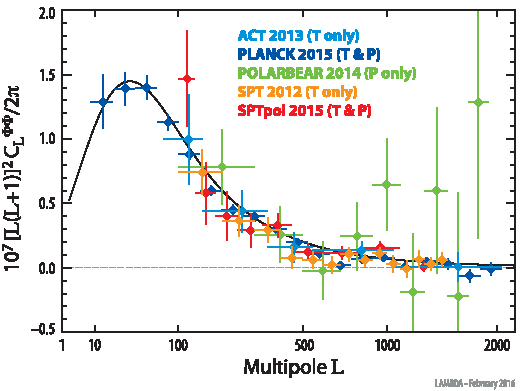
\includegraphics[width=0.85\textwidth]{Chapter1/Images/lensing_power_2016feb}
\caption{Status of CMB lensing measurements as of February 2016. Band powers shown in the plot are from ACT, \textit{Planck} full mission, POLARBEAR, SPT, and SPTPol. The black solid line represents the theoretical lensing power spectrum for the best-fit \gls{LCDM} parameters obtained from the \textit{Planck} 2015 temperature and polarization data. The figure is taken from the Legacy Archive for Microwave Background Data Analysis (LAMBDA) website (\url{http://lambda.gsfc.nasa.gov}). \label{fig:cmb_obs}}
\end{figure}

\myparagraph{Current status of observations}
\gls{CMB} lensing is a fast evolving field of research. The first observational hints of the lensing effects on \gls{CMB}
were found by \cite{Smith2007} and \cite{Hirata2008}, who cross-correlated properly filtered \gls{CMB} maps obtained from
\gls{WMAP} with external \gls{LSS} tracers. On the other hand, the first direct evidence of a preference for a lensed
\gls{CMB} is due to \cite{Reichardt2009} who combined \gls{ACBAR} and \gls{WMAP} data. With the advent of the high
sensitivity small scale \gls{CMB} temperature experiment such as \gls{ACT} \citep{Das2011} and \gls{SPT} 
\citep{Keisler2011}, the \gls{CMB} lensing potential reconstruction has become truly feasible for the first time, with reported detection significance around $\sim4-6\sigma$. The next step forward in \gls{CMB} lensing science has 
been made by the Planck team who detected the \gls{CMB} lensing power spectrum at a significance of about
$25\sigma$ and reconstructed an almost full-sky lensing map using only temperature data 
\cite{Ade2014c}.\footnote{Consider that the \textit{Planck} satellite is as sensitive to \gls{CMB} lensing as \gls{COBE} was to \gls{CMB} temperature fluctuations: $T:\kappa = $ COBE : Planck.} The first \gls{CMB} lensing measurements using polarization data have been recently 
reported by POLARBEAR \citep{Ade2014e}, SPTPol \citep{Story2015}, and \textit{Planck} \citep{PlanckCollaboration2015}: recent measurements are reported in Fig.~\eqref{fig:cmb_obs}.

\subsection{LSS lensing}
\label{sec:lsslens}
CMB photons are not the only ones that experience gravitational deflection by the intervening \gls{LSS}. 
Galaxy photons are also affected by weak lensing which causes (i) the distortion the \emph{shape} of galaxy images, and (ii) a change in their \emph{magnitude} and \emph{size} \citep{Bartelmann2001}: these 
two main effects are at the core of \gls{WL} measurements. Here, we focus on the relationship between the observables and the cosmological signal in \gls{WL}. 

\myparagraph{Shear measurements}
The most common quantity inferred from observations is the shear of galaxy images.
In the weak lensing limit ($|\gamma|,|\kappa|\ll1$), the shear can be directly estimated from the 
\emph{observed ellipticity} $\hat{\epsilon}$ as follows
%
\be
\epsilon = \gamma + \epsilon_{\rm{int}},
\ee
%
where $\epsilon_{\rm{int}}$ is the intrinsic ellipticity of source galaxies, for which current observations 
suggest $\sigma_{\rm{int}} = \sqrt{\langle|\epsilon_{\rm int}|^2\rangle}\simeq 0.4$. Measurement of
galaxy ellipticities are also complicated by several observational systematics such as the point spread 
function of the instrument and the blurring caused by atmosphere which have to be finely controlled.
Also in this case, what the theory predicts is the statistical correlation of galaxy shears, i.e. the shear
power spectrum (or correlation function). The convergence (angular) power spectrum is equivalent to the
shear power spectrum in the weak lensing limit, i.e. $C_{\ell}^{\kappa\kappa}\simeq C_{\ell}^{\gamma\gamma}$. Moreover, radial information can be used to perform a tomographic analysis of the \gls{WL}
signal by measuring the galaxy shear in redshift slices. Considering two redshift bins $i$ and $j$, with 
associated radial distribution of sources $\frac{\diff N_{i,j}}{\diff z}$, we  can write the tomographic 
cross-power spectra in different bins as 
%
\be
\langle \kappa^i_{\ell m}\kappa^j_{\ell' m'}\rangle = \delta^K_{\ell\ell'}\delta^K_{mm'}C^{\kappa^i\kappa^j}_{\ell},
\ee
%
which can be related to theory through \cite{}
%
\be
\label{eq:lens_spectra}
C_{\ell}^{\kappa^i\kappa^j} = 
\begin{cases}
\int_0^{\infty} \diff\chi \frac{W_i^{\kappa}(\chi)W_j^{\kappa}(\chi)}{f_K^2(\chi)} P_{\delta\delta}\biggl(\frac{\ell}{f_K(\chi)}, \chi \biggr) \\
\int_0^{\infty} \frac{\diff z}{H(z)} \frac{W_i^{\kappa}(z)W_j^{\kappa}(z)}{f_K^2(z)}P_{\delta\delta}\biggl(\frac{\ell}{f_K(z)},z \biggr).\\
\end{cases}
\ee
%
We recall that Eq.~\eqref{eq:lens_spectra} assumes both Limber and Born approximations. The observed 
auto-power spectra also include a shot-noise term due to random galaxy shape, 
$C_{\ell}^{\kappa^i\kappa^j} \to C_{\ell}^{\kappa^i\kappa^j} + \delta_{ij}\sigma^2_{\rm int}/\bar{n}_i$, 
where $\bar{n}_i$ is the average number of galaxies per steradian in the $i$-th redshift bin: a large 
number of sources increases the statistics, hence lowering the noise level.
If we decompose the shear into a tangential and cross component as
%
\begin{align}
\gamma_t &\equiv -\text{Re}[\gamma e^{-2i\phi}],\\
\gamma_{\times} &\equiv -\text{Im}[\gamma e^{-2i\phi}],
\end{align}
%
we can obtain a rotationally invariant linear combination of the cross-correlation functions of $\gamma_{\times}$ and $\gamma_t$  as follows:
%
\be
\begin{split}
\xi^{ij}_{\pm}(\theta) &\equiv \langle \gamma_t(0)\gamma_t(\bm{\theta}) \rangle \pm \langle \gamma_{\times}(0)\gamma_{\times}(\bm{\theta}) \rangle \\
&= \frac{1}{2\pi}\int_0^{\infty} \diff\ell\,\ell C_{\ell}^{\kappa^i\kappa^j} J_{0/4}(\ell\theta),
\end{split}
\ee
%
where the Bessel function $J_0$ ($J_4$) refers to the correlation function $\xi_+$ $(\xi_-)$. A common
estimator of the shear correlation function is \citep{}
%
\be
\label{eq:lens_est}
\hat{\xi}_{\pm}(\theta) = \frac{\sum_{ij}w_iw_j [e_t(\theta_i)e_t(\theta_j) \pm e_{\times}(\theta_i)e_{\times}(\theta_j)]}{\sum_{ij}w_iw_j},
\ee
%
where all galaxy pairs $(i,j)$ separated by an angular distance $|\theta_i-\theta_j|\in \theta$ contribute to
the same angular bin with their respective weights $(w_i, w_j)$. 

An important systematic effect that has
an impact on the above estimator is the intrinsic galaxy alignments due to tidal forces \citep{Hirata2004}. 
In fact, Eq.~\eqref{eq:lens_est} estimates $\langle\hat{\xi}_{\pm}\rangle = \xi_{\pm}+\xi_{\pm}^{\rm{II}}+\xi_{\pm}^{\rm{GI}}$, where $\xi_{\pm}^{\rm{II}}$
measures correlation between the intrinsic ellipticities of neighboring galaxies (known as ${\rm{II}}$) and 
$\xi_{\pm}^{\rm{II}}$ is sensitive to correlation between foreground Galaxy Intrinsic ellipticity and 
background galaxy shear (known as ${\rm{GI}}$). The modeling of galaxy alignment is a very active and
debated area of research, see \citet{Kirk2015} for a review. 

Intrinsic alignments represent a potential contaminant also to \gls{CMB} lensing-galaxy lensing cross-correlation measurements, entering the 2-point function as a
$\langle \kappa_{\rm CMB}{\rm I}\rangle$ term. \citet{Hand2015} measured for the first time the 
cross-correlation between the \gls{ACT} \gls{CMB} lensing and the galaxy convergence of \gls{CFHT} Stripe 82 
(CS82) and reported a lower amplitude with respect to the expect signal. \citet{Troxel2014} showed that intrinsic
alignment contamination could account for a $\approx 15\%$ reduction of the observed discrepancy; 
these findings have been later confirmed by \citet{Chisari2015} who modeled the impact of the intrinsic 
alignment with a model based on early-type\footnote{In this context it means \emph{red} galaxies.} galaxy population to 
\gls{CMB} 
lensing measurements, pointing out that at $z\gtrsim 1.2$ alignments remain largely unconstrained. 
\citet{Larsen2015} have considered the impact of intrinsic alignments of spiral galaxies on the \gls{CMB} 
lensing-galaxy lensing cross-correlation using the quadratic alignment model, finding the signal to be
similar in shape with respect to the linear model but with opposite sign, hence it can potentially reduce
the overall impact.

\myparagraph{Magnification bias}
The size amplification is called \emph{magnification} and leads to a fluctuation in the size and the flux of 
individual galaxies. Two competing effects are at play: one one hand \gls{WL} of photons stretches the 
observed area and \emph{dilutes} the number density, on the other it changes the \emph{apparent 
brightness} and allows galaxies in the survey. In a flux-limited survey, the number density of background 
galaxies is expected to be affected through magnification effects due to the foreground galaxy distribution. 
Let us see how.

In presence of lensing the galaxy flux is magnified by $f^{\rm{obs}} = \mu f^s$, where $f^{\rm{obs}}$ and
$f^s$ are is the observed and intrinsic galaxy flux respectively. 
In the \gls{WL} limit it can be shown that $N(>S)$,
the intrinsic counts of sources with observed flux greater than $S$, is related to the cumulative source 
counts $\tilde{N}(>S)$ observed in a given direction through \citep{Bartelmann2001}
%
\be
\tilde{N}(>S,\nver) = \mu^{\alpha-1}(\nver)N(>S).
\ee
%
Here, $\alpha$ is the logarithmic slope of the cumulative number counts of galaxies at the faint end, 
$\alpha=\frac{\diff\log{N(>S)}}{\diff S}|_{S_{\rm min}}$. Thus, if $\alpha > 1$ ($\alpha<1$), the observed number 
density of objects is enhanced (decreased) by lensing: this effect is the so-called 
\emph{magnification (anti-)bias}. Since $|\kappa|\ll 1$, the magnification $\mu$ can be approximated as $\mu \approx 1 + 2(\alpha-1)\kappa$ and the observed number density of galaxies is modulated by the foreground matter distribution as
%
\be
\label{eq:lens_magbias}
\begin{split}
\delta_g^{\rm{obs}}(\nver,z) &\simeq \delta_g^{\rm{cl}}(\nver,z) + 2(\alpha(z)-1)\kappa(\nver,z) \\
&= \delta_g^{\rm cl}(\nver,z) + \delta_g^{\mu}(\nver,z),
\end{split}
\ee
% 
where $\delta_g^{\rm{cl}}(\nver,z)$ is the intrinsic galaxy clustering term.
By substituting in Eq.~\eqref{eq:lens_magbias} the expression for the convergence $\kappa$ - of the sources in the redshift bin around $z_i$ - we get
%
\be
\delta^{\mu}_{\rm g}(\nver,z) = \frac{3\Omega_{\rm m}}{2c}\frac{H_0^2}{H(z)}(1+z)\chi(z) \int_z^{\infty}dz'\,\biggl(1-\frac{\chi(z)}{\chi(z')}\biggr)(\alpha(z')-1)\frac{dN}{dz'}.
\ee
%
Cosmic magnification measurements can be carried out by correlating the angular positions of 
background and foreground galaxy populations (see \citet{Scranton2005,Gonzalez-Nuevo2014}) and by 
counting galaxies \citep{Negrello2010}. Magnification bias can be either a source of information 
\citep{Hildebrandt2013} or a 
nuisance depending on the analysis performed and it can lead to substantial biases if not properly 
accounted for, as shown for \gls{CMB} lensing-galaxy density \citep{Bianchini2015} and \gls{iSW} 
(\gls{CMB} temperature-galaxy density) measurements \citep{LoVerde2007}.
The high-$z$ \gls{DSFG} detected by Herschel have a steep integrated number counts 
at the limiting flux, hence are potentially sensitive to the magnification bias as we will see in Ch.~\eqref{ch:xc1}.





\chapter{CMB-LSS cross-correlation: statistics and datasets}
\label{ch:statsdata}
\setlength{\epigraphwidth}{.57\textwidth}
\begin{epigraphs}
\qitem{\textit{Statistics: the mathematical theory of ignorance.}}%
 {---\textsc{Morris Kline}}
\end{epigraphs}
Cosmology is intrinsically entwined with statistics. There are threefold reasons for this. Firstly, given the huge size of cosmological structure it is impossible to follow the evolution of all components in a deterministic way. Secondly, we do not observe  along a single spatial hyper-surface, rather we have direct observational access to our past light-cone, which means that we see objects at different stages of their evolution. Thirdly the generation of primordial inhomogeneities is an intrinsic stochastic process and as such, we can just predict the statistical properties of cosmological fields (such as the matter density contrast $\delta$ or the intensity of \gls{CMB} temperature fluctuations). The main implication of these remarks is that we should model the observable Universe as a stochastic \emph{realization} of a stochastic \emph{ensemble}. Moreover, in the vanilla inflationary framework, the initial perturbations are Gaussian and adiabatic meaning that the study of \gls{GRF}, with a specific focus on isotropic and homogeneous ones, is pivotal in cosmology. 

This chapter mainly deals with the methodology at the core of the analyses presented in this thesis and with the exploited datasets. We start by describing cosmological random fields with a special focus on the mathematics on the sphere. Then, we discuss the spectral estimation problem in the light of cosmological surveys, while in the last part of the chapter we present the \textit{Planck} and \textit{Herschel} datasets. 


\section{Random Fields}
\label{sec:RF}

\subsection{3D Random Fields}
We can describe a perturbation (calculated at a given time $t$) as a random field $f(\bm{x})$, which basically means that we assign a random number at each point $\bm{x} \in \mathbb{R}$ according to a probability density function $\text{P}[f(\bm{x})]$.\footnote{We will consider \emph{centered} field, i.e. $\langle f(\bm{x})\rangle=0$ for the sake of clarity. This is not an issue since the mean can always be subtracted from the field.} Here, $\text{P}[f(\bm{x})]$ is a distribution that gives the probability of realizing a particular field configuration.\footnote{The probability that the field $f$ will have a given configuration between $f(\bm{x})$ and $f(\bm{x})+\diff f(\bm{x})$ is calculated as $\diff P=\text{P}[f(\bm{x})]\Pi_{\bm{x}}\diff f(\bm{x})\equiv \text{P}[f(\bm{x})]\mathcal{D}f$.} Strictly speaking, a random field is a collection of $N$ random variables $f(\bm{x}_i)$ with $x_i \in \mathbb{R}^n$; the set of functions is called an \emph{ensemble} while each individual function represents a \emph{realization} of the ensemble. 

The correlators of the fields are the expectation values of the product of the field at different locations (and times). The \gls{2PCF} is defined~by
%
\be
\label{eq:RF_2point}
\xi(\bm{x},\bm{y}) \equiv \langle f(\bm{x})f(\bm{y})\rangle = \int \mathcal{D}f\, \text{P}[f]f(\bm{x})f(\bm{y}),
\ee
%
where the integral is a functional integral (or path integral) over the field configurations. The requirements of statistical isotropy and homogeneity translate into the following constraints on the correlation function: $\xi(\bm{x},\bm{y})=\xi(R^{-1}\bm{x},R^{-1}\bm{y})$ for the former and $\xi(\bm{x},\bm{y})=\xi(\bm{x}-\bm{y})$ for the latter, where $R$ is a generic rotation matrix. Combining the two together we find that the \gls{2PCF} only depends on the distance between points, i.e. $\xi(\bm{x},\bm{y}) = \xi(|\bm{x}-\bm{y}|)$. The same calculations can be performed in the harmonic domain by Fourier transforming the field adopting the following convention:
%
\be
f(\bm{k}) = \int \diff^3x\, f(\bm{x})e^{-i\bm{k}\cdot\bm{x}} \quad \text{and} \quad f(\bm{x}) = \int \frac{\diff^3k}{(2\pi)^{3}}f(\bm{k})e^{i\bm{k}\cdot\bm{x}}
\ee
%
Generically the Fourier transform is complex but for real valued fields we have that $f(\bm{k}) = f^*(-\bm{k})$. Then, the \gls{2PCF} in Fourier space than reads as
%
\be
\begin{split}
\langle f(\bm{k})f^*(\bm{k'}) \rangle &= (2\pi)^3 \delta^D(\bm{k}-\bm{k'}) \frac{2\pi^2}{k^3}\mathcal{P}_f(k)\\
&= (2\pi)^3 \delta^D(\bm{k}-\bm{k'}) P_f(k)
\end{split}
\ee
%
where $\mathcal{P}_f(k)$ is the \emph{dimensionless power spectrum} and the homogeneity and isotropy are enforced by the delta function and the dependence only on the module of $k$. The \gls{2PCF} and the power spectrum are a Fourier transform pairs:
%
\be
\label{eq:RF_xipk}
\begin{split}
\xi(\bm{x},\bm{y}) = \langle f(\bm{x})f(\bm{y})\rangle &= \int \frac{\diff^3 k}{(2\pi)^{3}}\frac{\diff^3 k'}{(2\pi)^{3}} \langle f(\bm{k})f^*(\bm{k'})\rangle e^{i\bm{k}\cdot\bm{x}}e^{i\bm{k'}\cdot\bm{y}} \\
&= \frac{1}{4\pi}\int \diff\log{k}\, \mathcal{P}_f(k)\int \diff \Omega e^{i\bm{k}\cdot(\bm{x}-\bm{y})}.
\end{split}
\ee
%
After the angular integration, Eq.~\eqref{eq:RF_xipk} reduces to
%
\be
\xi(\bm{x},\bm{y}) = \int \diff\log{k} \mathcal{P}_f(k) j_0(k|\bm{x}-\bm{y}|),
\ee
%
where $j_0(x) = \sin{x}/x$ and the variance is computed as the \gls{2PCF} at zero-lag,
%
\be
\sigma^2 = \xi(0) = \int \diff\log{k}\, \mathcal{P}_f(k).
\ee
%
Higher-order correlations can be evaluated by averaging the product of $n$ fields; some of the most studied polyspectra are the 3PCF or \emph{bispectrum}
%
\be
\langle f(\bm{k}_1)f(\bm{k}_2)f(\bm{k}_3)\rangle = (2\pi)^3 B(\bm{k}_1,\bm{k}_2,\bm{k}_3)\delta^D(\bm{k}_1+\bm{k}_2+\bm{k}_3),
\ee
%
and the 4PCF or \emph{trispectrum}
%
\be
\langle f(\bm{k}_1)f(\bm{k}_2)f(\bm{k}_3)f(\bm{k}_4)\rangle = (2\pi)^3 T(\bm{k}_1,\bm{k}_2,\bm{k}_3\bm{k}_4)\delta^D(\bm{k}_1+\bm{k}_2+\bm{k}_3+\bm{k}_4).
\ee
%

\myparagraph{Gaussian Random Field}
This class of random fields is of particular relevance in cosmology due to the high-level of Gaussianity predicted by inflation for primordial fluctuations. For (homogeneous and isotropic) \gls{GRF}, $\text{P}[f(\bm{x})]$ is a Gaussian functional of $f$ fully characterized by its power spectrum\footnote{Since the mean is zero.}, or by the \gls{2PCF} equivalently. If we discretize the field in $N$ pixels and represent it  as a collection of $f_i=f(\bm{x}_i)$ in a $N$-dimensional vector $\bm{f}=[f_1,f_2,\dots,f_N]^T$, the multivariate joint probability distribution of the \gls{GRF}  has the following form
%
\be
\text{P}[\bm{f}] \propto \frac{e^{-f_i \text{C}^{-1}_{ij}f_j}}{\sqrt{\text{det}(\text{C})}},
\ee
%
where C$_{ij}=\langle f_i f_j\rangle$ is the covariance matrix. Since the Gaussian is even under parity around the mean, any odd expectation value vanishes, e.g. $\langle f(\bm{x_1})f(\bm{x_2})f(\bm{x_3})\rangle = 0$, while any even higher-order correlation function can be written as sum of \gls{2PCF} products: this result is known as \emph{Wick's theorem} (or Isserlis theorem) and can be expressed as 
%
\be
\langle f(\bm{x_1})f(\bm{x_2})f(\bm{x_3})f(\bm{x_4})\dots\rangle = \sum \text{All possibile 2-point contractions}.
\ee
%

\subsection{Fields on the sphere}
\label{sec:harmanalysis}
Nearly all cosmological observations, from CMB to galaxy surveys, provide us with a sampling of 3D random fields projected on the sphere, mostly in the form of two-dimensional sky-maps.\footnote{This especially applies when distance information about the sources is unavailable, nevertheless the quantity of interest can always be projected on the sphere, as is the case for tomographic analyses of \gls{LSS}.}
The information content hidden in such maps is usually probed by means of harmonic analysis on the sphere. A popular observable that characterizes the statistical properties of a given cosmic field is the
angular power spectrum $C_{\ell}$ and its reconstruction enables a direct comparison between
models and data.

It is common practice to decompose the observed field $X(\nver)$ into spherical harmonics, a frequency-space orthonormal basis for square-integrable, i.e. $\int_{\mathbb{S}^2}\diff \Omega |X(\nver)|^2 < \infty$, as:
%
\begin{equation}
X(\nver) = \sum_{\ell=0}^{\infty} \sum_{m=-\ell}^{\ell} x_{\ell m}Y_{\ell m}(\nver),
\label{eqn:spharm}
\end{equation}
%
where the spherical harmonic coefficients are given by
%
\begin{equation}
\label{eqn:sphcoeff}
x_{\ell m} = \int_{\mathbb{S}^2}X(\nver)Y^*_{\ell m}(\nver)d\Omega.
\end{equation}
%
The spherical harmonics $Y_{\ell m}$ are the eigenfunctions of the Laplacian on the sphere $\nabla^2_{\mathbb{S}^2}=\frac{1}{\sin\theta}\frac
{\partial}{\partial\theta}
\left(\sin\theta\frac{\partial}{\partial\theta}\right)+\frac{1}{\sin^2\theta}\frac{\partial^2}{\partial\varphi^2}$, and are described by two integers, the \emph{multipole} $\ell$ and the azimuthal parameter $m$ that satisfy $\nabla^2_{\mathbb{S}^2} Y_{\ell m} = -\ell(\ell+1)Y_{\ell m}$ and $\partial_{\varphi} Y_{\ell m}= imY_{\ell m}$. We recall below some useful properties:
%
\begin{align}
\int_{\mathbb{S}^2} \diff\Omega\, Y_{\ell m}(\nver)Y^*_{\ell' m'}(\nver) &= \delta^K_{\ell\ell'}\delta^K_{mm'} &\text{Orthonormality}\\
\sum_{\ell m} Y_{\ell m}(\nver)Y^*_{\ell m}(\nver') &= \delta^D(\nver-\nver') &\text{Completeness} \\
\sum_m Y_{\ell m}(\nver)Y^*_{\ell m}(\nver') &= \frac{2\ell+1}{4\pi} P_{\ell}(\nver\cdot\nver') &\text{Addition Theorem} 
\end{align}
%
where $P_{\ell}(x)$ are the usual Legendre polynomials. The phase of $Y_{\ell m}$ can be chosen such  that $Y^*_{\ell m} = (-1)^mY_{\ell\, -m}$, so that for a real valued field we have $x^*_{\ell m}=(-1)^m x_{\ell\,-m}$.

Under the assumption of statistical isotropy, for a finite variance field, the mean of the spherical harmonic coefficients is $\langle x_{\ell m}\rangle = 0$, while their covariance is given by 
%
\be
\langle x_{\ell m} x^*_{\ell' m'}\rangle = C^{XX}_{\ell}\delta^K_{\ell\ell'}\delta^K_{mm'},
\ee
%
where $C_{\ell}^{XX}$ is the \emph{angular power spectrum} of $X$ which is related to the angular \gls{2PCF} $C^{XX}(\theta)$ through (see Eq.~\eqref{eq:c2cl} for the derivation)
%
\begin{align}
C^{XX}(\theta) &= \sum_{\ell}\frac{2\ell+1}{4\pi}C_{\ell}^{TT}P_{\ell}(\nver\cdot\nver')\\
C_{\ell}^{XX} &= 2\pi\int_{-1}^{1} \diff\cos{\theta}\, C^{XX}(\theta)P_{\ell}(\cos{\theta}).
\end{align}
%
It is also possible to expand the product of two spherical harmonics in terms of spherical harmonics as 
%
\be
Y_{\ell m}(\nver)Y_{\ell'm'}(\nver) = \sum_{LM} \sqrt{\frac{(2\ell+1)(2\ell'+1)(2L+1)}{4\pi}} \wig{\ell}{\ell'}{L}{m}{m'}{M}\wig{\ell}{\ell'}{L}{0}{0}{0} Y_{LM}^*(\nver),
\ee
%
where the strange quantities in parenthesis that we have introduced are called the Wigner $3j$ symbols \citep{Varshalovich1988}. Integrating the above expression over the whole sphere one finds the \emph{Gaunt relation}:
%
\be
\begin{split}
\mathcal{G}^{\ell\ell'L}_{mm'M} &\equiv \int_{\mathbb{S}^2}\diff\Omega\,Y_{\ell m}(\nver)Y_{\ell'm'}(\nver)Y_{LM}(\nver)\\
&= \sqrt{\frac{(2\ell+1)(2\ell'+1)(2L+1)}{4\pi}} \wig{\ell}{\ell'}{L}{0}{0}{0}\wig{\ell}{\ell'}{L}{m}{m'}{M}.
\end{split}
\ee
%
Basically, Wigner $3j$ matrices are a rescaling of the Clebsch-Gordan coefficients and describe the quantum mechanical composition of two angular momentum eigenstates into a third one.
The selection rules for Wigner $3j$ symbols, i.e. when they are non-null, are given by
%
\begin{align}
\ell + \ell' + L & \,\,\text{is even,} \\
|\ell-\ell'| \le L &\le \ell+\ell' \\
m + m' + M& = 0.
\end{align}
%
These objects are somewhat nasty to calculate and are at the core of the \gls{PCL} methods to calculate the masking induced mode-coupling, as we will see in Sec.~\eqref{sec:ps_est}. Harmonic calculations on the sphere can be performed on the computer with standard packages for \gls{CMB} data analysis such as \texttt{HEALPix}\footnote{\url{http://healpix.sourceforge.net}} \citep{Gorski2005a} and \texttt{S}$^2$\texttt{HAT} \citep{Stompor2011}. The basic idea is to tesselate the sphere according to some pixelization scheme and to discretize the function into maps. As an example, for \texttt{HEALPix}, the resolution of the grid is controlled by the parameter $N_{\rm{side}}=2^k$ (where $k \in \mathbb{N}$) which fixes the total number of pixels $N_{\rm{pix}}=12N_{\rm{side}}^2$. In particular, spherical harmonic transforms in Eq.~\eqref{eqn:sphcoeff} are operatively estimated as 
%
\be
x_{\ell m} \approx \Omega_p \sum_p X(p)Y^*_{\ell m}(p),
\ee
%
where $\Omega_p = \frac{4\pi}{N_{\rm{pix}}}$ is the solid angle subtended by each pixel $p$. Another complication that arises from pixelization is that we only know the value of the field averaged over the pixel area: the effect is an amount of degradation of the information below a certain scale set by the size of the pixel (basically it acts as a low-pass filter). A way to account for this bias is to deconvolve the reconstructed spectrum for the \emph{pixel window function} $p_{\ell}$ ($C_{\ell}^{\rm{obs}} = p^2_{\ell}C_{\ell}$).

Before concluding this subsection, let us take a look at the near future: most of the upcoming cosmological surveys will carry out large and deep observations of the sky, providing both angular and redshift information about the cosmic fields. Thus, a formalism  
for analyzing function on the 3D \emph{ball} -  a family of concentric spheres (shells) indexed by a continuos radial parameter, such as the redshift $z$ - will be required. Tomographical analyses (see Ch.~\eqref{ch:xc2}) represent a first step in this direction: the idea is to slice the data in redshift bins and then perform the usual 2D spherical analysis. A natural decomposition scheme for full-3D analyses is given by the spherical Fourier-Bessel formalism, while extensions to wavelets \citep{Lanusse2012,Leistedt2012} and radial 3D needlets \citep{Durastanti2014} have also been investigated.

\subsection{Projected fields}
Let us now work out the connection between a 3D field $X^{\rm 3D}(\bm{x})$ and its 2D counterpart $X^{\rm 2D}(\nver)$, projected
on the sphere and integrated along the light-cone according to some arbitrary weight function $W^X(\chi)$:\footnote{To avoid a crowding of equations we restrict to the case of a flat Universe, so that $f_K(\chi)=\chi$.}
%
\begin{equation}
X^{\rm 2D}(\nver) = \int_0^{\infty} \diff\chi\,  W^X(\chi) X^{\rm 3D}(\chi\nver,\chi).
\end{equation}
%
Using the Rayleigh's expansion
\begin{equation}
e^{i\mathbf{k}\cdot\nver\chi(z)} = 4\pi\sum_{\ell m}i^{\ell}j_{\ell}(k\chi)Y^*_{\ell m}(\kver)Y_{\ell m}(\nver),
\end{equation}
we can Fourier transform the 3D field $X^{\rm 3D}(\chi\nver,\chi)$ and obtain
%
\begin{equation}
\begin{split}
X^{\rm 3D}(\chi\nver, \chi) &= \int \frac{\diff^3k}{(2\pi)^3}\,X^{\rm 3D}(\mathbf{k}, \chi) e^{i\mathbf{k}\cdot\nver\chi} \\
&=4\pi\sum_{\ell m}i^{\ell}\int \frac{\diff^3k}{(2\pi)^3}\,X^{\rm 3D}(\mathbf{k}, \chi) j_{\ell}(k\chi)Y^*_{\ell m}(\kver)Y_{\ell m}(\nver).
\end{split}
\end{equation}
%
In this way, the projected field becomes
%
\begin{equation}
X^{\rm 2D}(\nver)= 4\pi\sum_{\ell m}i^{\ell}\int \diff\chi W^X(\chi) \int \frac{\diff^3k}{(2\pi)^3}X^{\rm 3D}(\mathbf{k}, \chi) j_{\ell}(k\chi)Y^*_{\ell m}(\kver)Y_{\ell m}(\nver),
\end{equation}
%
and the spherical coefficients read as 
\begin{equation}
x_{\ell m} =4\pi i^{\ell} \int \diff\chi\, W^X(\chi) \int \frac{\diff^3k}{(2\pi)^3}\,X^{\rm 3D}(\mathbf{k}, \chi) j_{\ell}(k\chi)Y^*_{\ell m}(\kver).
\end{equation}
We calculate the angular cross power spectrum $C_{\ell}^{XY}$ by taking the ensemble average of $\langle x_{\ell m}y^*_{\ell m}\rangle $ as 
%
\begin{equation}
\begin{split}
C_{\ell}^{XY} =\:&  (4\pi)^2 \int \diff\chi\, W^X(\chi)\int \diff\chi'\, W^X(\chi')\\
&\times \int\frac{\diff^3k}{(2\pi)^3}\frac{\diff^3k'}{(2\pi)^3}\langle X^{\rm 3D}(\mathbf{k}, \chi) Y^{\rm 3D*}(\mathbf{k'}, \chi') \rangle 
 j_{\ell}(k\chi)j_{\ell'}(k'\chi')Y^*_{\ell m}(\kver)Y_{\ell' m'}(\kver') \\
=\:& (4\pi)^2 \int \diff\chi\, W^X(\chi)\int \diff\chi'\, W^Y(\chi')\int\frac{\diff^3k}{(2\pi)^3}  P_{XY}(k;\chi,\chi') j_{\ell}(k\chi)j_{\ell'}(k\chi')Y^*_{\ell m}(\kver)Y_{\ell' m'}(\kver) \\
=\:& \frac{2}{\pi}\int \diff\chi\, W^X(\chi)\int \diff\chi'\, W^Y(\chi')\int k^2\diff k\,  P_{XY}(k;\chi,\chi') j_{\ell}(k\chi)j_{\ell}(k\chi') 
\end{split}
\end{equation}
%
where we used the definition of (isotropic) 3D cross-power spectrum $\langle X(\mathbf{k}, \chi) Y^*(\mathbf{k'}, \chi')\rangle= (2\pi)^3\delta^D(\kvec-\kvec')P_{XY}(k;\chi,\chi')$ and the orthonormality condition of spherical harmonics. Summing up, the \emph{exact} relation is
%
\begin{equation}
\label{eq:clexact}
C_{\ell}^{XY} = \frac{2}{\pi}\int \diff\chi\, W^X(\chi)\int \diff\chi'\, W^Y(\chi')\int k^2\diff k\,  P_{XY}(k;\chi,\chi') j_{\ell}(k\chi)j_{\ell}(k\chi').
\end{equation}
% 
\myparagraph{Limber approximation}
The Limber approximation \citep{Limber1953a} is a handy tool whenever integrals of Bessel functions appear.
When deriving it, one usually assumes small angular separations (or large multipoles $\ell$) and that some of the integrand functions vary slower with respect to others. The idea is that if $f(x)$ is a smooth function, then $\int_0^{\infty} \diff x f(x)J_{\nu}(x) = f(\nu) + \mathcal{O}(1/\nu^2)$, where $\nu \equiv \ell + 1/2$; this can be written in the following form
%
\begin{equation}
\frac{2}{\pi}\int k^2\diff k\, f(k) j_{\ell}(k\chi)j_{\ell}(k\chi') = \frac{\delta^D(\chi-\chi')}{\chi^2} f\biggl(\frac{\nu}{\chi}\biggr)\biggl[1+\mathcal{O}\biggl(\frac{1}{\nu^2}\biggr)\biggr],
\end{equation}
%
where the presence of the $\delta^D$ tells us that the integrand is dominated by the region $\chi \approx \chi'$, and the goodness of the approximation gets better as $\ell\to\infty$, i.e. the corrections are $\mathcal{O}(1/\nu^2)$ (see \citet{LoVerde2007}).
Substituting the above expression in Eq.~\eqref{eq:clexact} (and integrating out the $\delta^D$), one finds the Limber approximated angular power spectrum:
%
\be
\label{eq:cllimber}
C_{\ell}^{XY} = \int_0^{\infty} \frac{\diff\chi}{\chi^2}W^X(\chi)W^Y(\chi) P_{XY}\Biggl(\frac{\ell+\frac{1}{2}}{\chi},\chi\Biggr). 
\ee
%
In literature the power spectrum in Eq.~\eqref{eq:cllimber} is sometimes evaluated at $\nu = \ell$ (as will be the case in Ch.~\eqref{ch:xc1} and \eqref{ch:xc2}), which increase the error from $\mathcal{O}(\ell^{-2})$ to $\mathcal{O}(\ell^{-1})$. The approximation is correct to $\mathcal{O}(1\%)$ for $\ell \gtrsim 10$. An extended Limber approximation, in the sense that exploits higher-order terms in the Bessel integral expansion, has been developed by \citet{LoVerde2007}. For completeness, we write below the analogous of Eq.~\eqref{eq:cllimber} with the integration in redshift space:\footnote{In order to switch the Dirac delta from $\chi$ to $z$ recall that $\delta^D[g(x)]=\frac{\delta^D(x-x_0)}{|g'(x_0)|}$ where $x_0$ is the root of $g(x)$. In our case $g(z)=\chi(z)-\chi(z')=\int_0^z\frac{c\,dz''}{H(z'')}-\int_0^{z'}\frac{c\,dz''}{H(z'')}$, so that $g'(z)=\frac{c}{H(z)}$ and $\delta^D[\chi(z)-\chi(z')] = \frac{H}{c}(z')\delta^D(z-z')$}
\be
\label{eq:cllimber_z}
C_{\ell}^{XY} = \int_0^{\infty} \frac{\diff z}{c} \frac{H(z)}{\chi^2(z)}W^X(z)W^Y(z) P_{XY}\Biggl(\frac{\ell+\frac{1}{2}}{\chi(z)},z\Biggr). 
\ee
Recall that the comoving distances $\chi$ should be replaced by $f_K(\chi)$ for non-flat cosmologies and that Limber approximation is valid as long as (i) the sources stretch in a \emph{wide} range of distances $\Delta\chi$ and (ii) vary smoothly, i.e. $\ell/\chi\times\Delta\chi \gg 1$ (see \citet{Simon2007,Bernardeau2011}).

\section{Spectral estimation}
\label{sec:ps_est}
The scientific exploitation of any cosmological dataset is just the tip of the iceberg: the data analysis that allows us to extract science from observations is a complex and iterative process which requires both computational and physical solid skills. Having in mind the \gls{CMB} field, the reduction of a dataset usually can be split in the following sequence of steps:
\begin{itemize}
\item{\textbf{Pre-processing}: the goal is to prepare real data so that can be fed to the subsequent pipeline steps. Here, the raw time-ordered data (TOD) collected by the detectors are calibrated and the time-domain systematics are generally flagged and/or removed.}
\item{\textbf{Map-making}: after characterizing the instrument's noise specifics, the different frequency maps of the observed temperature and polarization are extracted from the cleaned TOD.}
\item{\textbf{Component separation}: the available spectral information is used to isolate the emission from all other (astrophysical) components in the data, hence singling out the \gls{CMB} signal. One of the outcome of this pipeline step is the production of ancillary data. Though not strictly correct, we can insert in this step the production of additional maps, such as the \gls{CMB} gravitational lensing convergence, derived from the $T$ and $P$ separated maps.}
\item{\textbf{Power spectrum estimation}: \gls{CMB} temperature $T$ and polarization $E$- and $B$- modes auto- and cross-power spectra are reconstructed from the maps, along with spectra of derived fields such as lensing $\kappa$.}
\item{\textbf{Parameter estimation}: the estimated set of \gls{CMB} power spectra is compared with the theoretical models to study the degeneracies in the parameter space and infer best-fit parameters, usually by means of Bayesian analysis.}
\end{itemize}

\subsection{Power spectrum estimators}
\label{sec:ps_est_master}
Throughout  my thesis I have mainly been involved with the last two steps of the \gls{CMB} pipeline, here I will focus on the power-spectrum estimation techniques: since the statistical properties of \gls{GRF} are completely described by their power spectra, spectral estimation is a pivotal step.

There exist a variety of well-established methods to recover the underlying angular spectra from observations. In principle, optimal maximum likelihood algorithms can be applied to the spectral estimation problem, assuming that the pixel-pixel covariance matrix is known. The idea behind these methods is the following: considering a data vector $x_i$ (e.g. the \gls{CMB} temperature in a given pixel) of length $N_d$ with the $x_i$ being Gaussian distributed, then the likelihood function reads as
%
\be
\mathcal{L}(C_{\ell}|\bm{x}) = \frac{\exp{\bigl(-\frac{1}{2}x^T C^{-1} x\bigr)}} {\sqrt{(2\pi)^{N_d} \text{det}(C)}}.
\ee
%
Here $C_{\ell}$ is the power spectrum to be estimated and the covariance matrix $C$ (in pixel space) can be written as the sum of signal $S_{ij}$ and noise $N_{ij}$ terms as $C_{ij}=\langle x_ix_j\rangle=S_{ij}(C_{\ell})+N_{ij}$. From this, maximum likelihood solution can be found iteratively with Newton-Raphson algorithm \citep{Bond1998} or with quadratic maximum likelihood estimators \citep{Tegmark1997}. Despite being optimal, these methods are computational expensive and require $\mathcal{O}(N_{\rm{pix}}^3)$ CPU time (as well as a good knowledge of the covariance matrix), and become prohibitively for datasets with $N_{\rm{pix}} \gtrsim 10^5$. 

As a result, \gls{PCL} techniques have emerged on the market, see \citet{Yu1969,Hauser1973,Wandelt2001,Hivon2001a,Efstathiou2004a}. The idea is to split the estimation of $C_{\ell}$ in two steps: a biased estimate $\tilde{C}_{\ell}$ of the power spectrum is first obtained, and then  corrected in the harmonic domain for all the different biasing effects such as the beam function, the pixelization, the mapmaking, and mode-mode coupling induced by masking. Schematically, the true power spectrum and the initial estimate are related by the mapping $\tilde{C_{\ell}}= f(C_{\ell})$, where the function $f$ encodes all the biasing effects. If we linearly expand it, we can rewrite the previous relation in matrix notation as $\langle\tilde{C}_{\ell'}\rangle \approx \sum_\ell \alpha_{\ell'\ell}C_{\ell} + \beta_{\ell'}$, where $\{\alpha_{\ell'\ell}, \beta_{\ell'}\}$ are the coefficients that approximate the effect of $f$, and then invert it to recover the true spectrum as $\hat{C}_{\ell'} = \alpha^{-1}_{\ell'\ell}(\tilde{C}_{\ell}-\beta_{\ell})$. 
The \gls{PCL} method is very fast, requiring $\mathcal{O}(N_{\rm{pix}}^{3/2})$ CPU time and it is nearly-optimal for temperature (and scalar fields) in practice.\footnote{The problem with the estimation of polarized spectra is the spurious mixing of $E$- and $B$-modes ($E$-to-$B$ leakage) that has to be taken into account. Several methods have been proposed to treat such effect, see \citet{Lewis2001,Bunn2003,Grain2009}.} Let us see the details of the method (for spin-0 fields).

From a statistical point of view, an unbiased estimator of the (cross-)angular power spectrum is given by (hereafter the hat $\hat{X}$ 
denotes  estimated quantities):
%
\begin{equation}
\label{eq:cl_est}
\hat{C}_{\ell}^{XY} = \frac{1}{2\ell+1}\sum_{m=-\ell}^{\ell} x_{\ell m}y_{\ell m}^*.
\end{equation}
%
%$\hat{C}_{\ell}$ can be shown to possess the minimal variance among the unbiased 
%estimators (in the sense that its variance reaches the Cram\`er-Rao lower bound).
Spherical harmonics are particularly appealing because they are statistically orthogonal for full-sky 
Gaussian-distributed sky-maps, i.e. the covariance is diagonal $\text{Cov}_{\ell \ell'}\propto \delta^K_{\ell
\ell'}$, and the power spectrum fully characterizes the behavior of the field. However, real-world observations have to deal with
a number of limitations and issues, such as the finite instrumental spatial resolution, the anisotropic 
noise, and asymmetric beam response. Moreover the incomplete sky coverage, motivated for example 
by foreground contamination or the instruments scanning strategy, induces a mode-coupling and a power leakage between 
different multipoles, as well as an overall downward shift of power \citep{Hivon2001a,Efstathiou2004a}. 
Consider a position dependent weighting scheme $W(\nver)$, i.e. the mask, whose harmonic expansion is $W(\nver)=\sum_{\ell m} w_{\ell m}Y^*_{\ell m}(\nver)$ and its power spectrum is $\mathcal{W}_{\ell}$. Then the pseudo-$x_{\ell m}$ of the masked field $\tilde{X}(\nver)=X(\nver)W(\nver)$ are given by:
%
\begin{equation}
\begin{split}
\tilde{x}_{\ell m} &= \int_{\mathbb{S}^2}X(\nver)W(\nver)Y^*_{\ell m}(\nver)d\Omega \\
&= \sum_{\ell'm'} x_{\ell'm'} \int\diff\Omega \, Y_{\ell'm'}(\nver) W(\nver)Y^*_{\ell m}(\nver)\\
&= \sum_{\ell' m'} K_{\ell m \ell' m' }[W] x_{\ell' m'},
\end{split}
\label{eqn:sphcoeffmask}
\end{equation}
%
where the kernel $K$  that describes the induced mode-coupling reads as
%
\be
K_{\ell m \ell' m' }[W]  \equiv (-1)^m \sum_{\ell'' m''} w_{\ell'' m''} \gaunt{\ell}{\ell'}{\ell''}{m}{m'}{m''}.
\ee
%
The well known \texttt{MASTER} \citep{Hivon2001a} (or \texttt{XSPECT}, the cross-spectra extension by \citet{Tristram2005}) approach to obtain unbiased but slightly sub-optimal multipole estimates relates the pseudo-spectrum 
%
\be
\tilde{C}^{XY}_{\ell} = \frac{1}{2\ell+1} \sum_m \tilde{x}_{\ell m}\tilde{y}^*_{\ell m}
\ee
%
to the underlying power spectrum $C_{\ell}$ as 
%
\begin{equation}
\label{eqn:pcl2cl}
\langle \tilde{C}^{XY}_{\ell}\rangle = \sum_{\ell'} M_{\ell\ell'} C^{XY}_{\ell'},
\end{equation}
%
where $M_{\ell\ell'}$ is the \emph{coupling matrix} 
%
\be
M_{\ell\ell'} = \frac{2\ell'+1}{4\pi} \sum_{\ell''} (2\ell''+1) \mathcal{W}_{\ell''} \wig{\ell}{\ell'}{\ell''}{0}{0}{0}^2
\ee
%
The finite size of the observed sky patch (of area $A_{\rm{obs}}$) approximately determines the smaller multipole that can be recovered, 
$\ell_{\rm{min}}\approx \pi/\sqrt{A_{\rm{obs}}}$, and the width of $M_{\ell\ell'}$, that characterizes the amount of mode-coupling.  
The basic idea is to invert eq.~\eqref{eqn:pcl2cl} in order to 
recover the underlying power spectrum, however for small sky fraction  $f_{\rm{sky}}=\frac{1}{4\pi}\int_{\mathbb{S}^2}W^2(\nver)d\Omega$, 
one needs to bin the pseudo-power spectrum and the coupling matrix, so that the estimator of the true
 cross-bandpowers $\hat{C}^{XY}_{L}$ writes
%
\begin{equation}
\label{eqn:master_xy}
\hat{C}^{XY}_{L} = \sum_{L' \ell}K^{-1}_{LL'}P_{L'\ell}\tilde{C}^{XY}_{\ell},
\end{equation}
%
where $L$ is the bandpower index and the binned coupling matrix can be written as
%
\begin{equation}
K_{LL'} = \sum_{\ell\ell'} P_{L\ell}M_{\ell\ell'}B^X_{\ell'}B^Y_{\ell'}p^2_{\ell'}F_{\ell'}Q_{\ell' L'}.
\end{equation}
%
Here $P_{L\ell}$ is the binning operator and $Q_{\ell L}$ is its reciprocal. To correct also for angular resolution, finite pixel size and filtering applied to TOD, we added to the binned coupling matrix the beam function (for the observed field $X$) $B^X_{\ell'}$, the pixel window function $p_{\ell}$, and the effective filtering function $F_{\ell'}$. When dealing with auto-power spectra of maps comprehensive of noise, Eq.~\eqref{eqn:master_xy} gets modified as
%
\begin{equation}
\label{eqn:master_xx}
\hat{C}^{XX}_{L} = \sum_{L' \ell}K^{-1}_{LL'}P_{L'\ell}(\tilde{C}^{XX}_{\ell} - \langle \tilde{N}^{XX}_{\ell} \rangle_{\rm{MC}}),
\end{equation}
%
where $\langle \tilde{N}^{XX}_{\ell} \rangle_{\rm{MC}}$ is the \gls{MC} estimate of the average noise pseudo-power spectrum.
If the true power spectrum varies slowly with respect to the coupling matrix and/or $f_{\rm{sky}}$ is large, eq.~\eqref{eqn:pcl2cl} becomes  
%
\begin{equation}
\label{eqn:fsky_app}
\langle \tilde{C}^{XY}_{\ell}\rangle \approx  C^{XY}_{\ell}  \sum_{\ell'} M_{\ell\ell'} = f_{\rm{sky}} C^{XY}_{\ell},
\end{equation}
%
which is the so-called $f_{\rm{sky}}$ approximation \citep{Komatsu2002a}. For the analyses discussed in Ch~\eqref{ch:xc1} and \eqref{ch:xc2} and performed during my Ph.D., I have developed a code to compute coupling matrices and estimate power spectra of spin-0 masked maps. The computational bottleneck is represented by the calculation of the Wigner $3j$ symbols: to this end, I have wrapped the FORTRAN rc3jj.f routine from the \texttt{SLATEC} library\footnote{\url{http://www.netlib.org/slatec/}} into flexible Python code which calculates the coupling matrix $M_{\ell\ell'}$, as well as other quantities, and can be efficiently interfaced with usual \texttt{HEALPix}-based codes (such as the Python implementation called \texttt{healpy}\footnote{\url{https://healpy.readthedocs.io/en/latest/}}). Just as an illustration and example of how a coupling matrix can appear, we anticipate here the mapping in the case of the H-ATLAS dataset considered in this analysis.
In the left panel of Fig.~\eqref{fig:master} we show the \textit{unbinned} coupling matrix $M_{\ell\ell'}$ computed for the H-ATLAS mask (shown in the right panel of Fig.~\eqref{fig:masks}) that tells us how the different harmonic modes are coupled to each other. As previously mentioned, the width of the diagonal is roughly determined by the sky coverage and mask topology: to highlight this aspect, we plot slices through $M_{\ell\ell'}$ (at fixed $\ell'$) in the right panel of Fig.~\eqref{fig:master}.

\begin{figure} %1
\centering % \begin{center}/\end{center} takes some additional vertical space
\includegraphics[width=\textwidth]{Chapter2/Images/master}
\caption{\emph{Left panel:} Coupling matrix $M_{\ell\ell'}$ evaluated for the H-ATLAS mask shown in Fig.~\eqref{fig:masks}. The main diagonal structure, whose width determines the extent of the mode-coupling, is visible. \emph{Right panel:} Slices through the coupling matrix shown in the left panel. \label{fig:master}}
\end{figure}

\subsection{Covariance estimators}
\label{sec:cov_est}
An estimate of the power spectrum means almost nothing without the associated covariance matrix. Error bars must be assigned to asses the quality or the significance of measurements and, for example, the full covariance matrix is needed to perform the further pipeline steps such as the parameter estimation. The covariance of the power spectrum estimator $\hat{C}_{\ell}^{XX}$ defined in Eq.~\eqref{eq:cl_est} is:\footnote{Assuming that the fields are Gaussian, hence neglecting the connected part $\langle  x_{\ell m}y^*_{\ell m}x_{\ell'm'}y^*_{\ell'm'}\rangle_c$.}
%
\be
\begin{split}
\cov(\hat{C}^{XY}_{\ell},\hat{C}^{XY}_{\ell'}) &= \langle (\hat{C}^{XY}_{\ell} - C^{XY}_{\ell}) (\hat{C}^{XY}_{\ell'} - C^{XY}_{\ell'}) \rangle \\
&= \frac{1}{(2\ell+1)(2\ell'+1)}\sum_{mm'} \langle x_{\ell m}y^*_{\ell m}x_{\ell'm'}y^*_{\ell'm'}\rangle - C^{XY}_{\ell}C^{XY}_{\ell'} -  \cancel{C^{XY}_{\ell}C^{XY}_{\ell'}}  \\
&\hphantom{=}+ \cancel{C^{XY}_{\ell}C^{XY}_{\ell'}}\\
&= \frac{1}{(2\ell+1)(2\ell'+1)}\sum_{mm'} \Bigl[\langle x_{\ell m}y^*_{\ell m} \rangle\langle x_{\ell' m'}y^*_{\ell' m'} \rangle  + \langle x_{\ell m}x_{\ell'm'} \rangle\langle y^*_{\ell m}y^*_{\ell' m'} \rangle \\
&\hphantom{=\frac{1}{(2\ell+1)(2\ell'+1)}\sum_{mm'} [}+ \langle x_{\ell m}y^*_{\ell' m'} \rangle\langle x^*_{\ell' m'}y^*_{\ell' m'} \rangle\Bigr] - C^{XY}_{\ell}C^{XY}_{\ell'}\\
&= \cancel{C^{XY}_{\ell}C^{XY}_{\ell'}} + \frac{C^{XX}_{\ell}C^{YY}_{\ell'}}{2\ell+1}\delta^K_{\ell\ell'} + \frac{C^{XY}_{\ell}C^{XY}_{\ell'}}{2\ell+1}\delta^K_{\ell\ell'} - \cancel{C^{XY}_{\ell}C^{XY}_{\ell'}} \\
&= \frac{\delta^K_{\ell\ell'}}{2\ell+1} \left[C^{XY}_{\ell}C^{XY}_{\ell'} + C^{XX}_{\ell}C^{YY}_{\ell'}\right]. 
\end{split}
\ee
%
Then, the cross- and auto-power spectrum variance associated to a given multipole are respectively
%
\begin{align}
\label{eq:thvar}
(\Delta C_{\ell}^{XY})^2 &= \frac{1}{2\ell+1}\left[(C^{XY}_{\ell})^2 + C^{XX}_{\ell}C^{YY}_{\ell}\right] \\
(\Delta C_{\ell}^{XX})^2 &= \frac{2}{2\ell+1}(C^{XX}_{\ell})^2,
\end{align}
%
with the last one being the same as Eq.~\eqref{eq:cmb_CV}. Let us make a couple of remarks. First of all, if the maps being analyzed are comprehensive of noise (as in the real-world), then the auto-power spectra appearing in the above equations must include a noise term, i.e. $C_{\ell}^{XX} \to C_{\ell}^{XX} + N_{\ell}^{XX}$. Secondly, in the incomplete sky case, things become much more nastier and a \emph{full} analytical treatment is virtually unfeasible. Several authors \citep{Efstathiou2004a,Tristram2005,Brown2005} have proposed analytic approximations if the underlying power spectra meet certain criteria, for example if they vary slow with respect to the coupling matrix. In the \emph{zeroth-order} approximate formula for power spectrum error bars, known as the Knox formula \citep{Knox1995}, the fractional error on $C_{\ell}$ typically scales as $1/\sqrt{f_{\rm{sky}}}$. Although it is helpful for an assessment of uncertainties, it is known to underestimate errors and does not account for the mode-mode coupling and the $E$-to-$B$ mixing. We will discuss in greater detail these approximations and compare different covariance estimators for cross-power spectra in Ch.~\eqref{ch:xc1}. The covariance can also be estimated numerically by means of MC simulations with resampling techniques. There exist different ways to calculate the covariance, each with their respective advantages and drawbacks. Here we list the most common  ones adopted in literature for cross-correlation analyses, mainly developed for \gls{iSW} studies, see \citet{Cabre2007,Giannantonio2008} for thorough discussions.

\begin{itemize}
\item{\textbf{\gls{MC} method 1}: Perhaps the most used estimator in literature, it consists in measuring the cross-power spectrum (or \gls{2PCF}) between $\Nsim$ random maps of field $X$, obtained from a fiducial model, and the observed maps of the field $Y$. This method is fast and straightforward to implement. \emph{Issues}: it is model-dependent (like all \gls{MC} approaches),  it does not account for the variance in the $Y$ maps (this is called the \emph{realization bias} since we have only one realization of the $Y$ field), and it assumes no cross-correlation between the fields (the so-called \emph{correlation bias}, but if the expected signal is weak, it should not represent a large bias).}
\item{\textbf{\gls{MC} method 2}: It tries to improve \gls{MC}1 by measuring the cross-power spectrum between random (\gls{MC} generated) maps of the $X$ field (from the underlying model) and random $Y$ field maps. \emph{Issues}: it is somewhat more time consuming and still model-dependent but has no dependence on any observed maps unlike the \gls{MC}1.}
\item{\textbf{Jack-knife (JK) method}: The idea is to divide the $Y$ field (e.g., the LSS tracer map) into $M$ patches to create $M$ subsamples (of approximately the same area) by neglecting each patch in turn and evaluating the covariance between them. \emph{Issues}: it underestimates the error, results are dependent on the size and number of discarded patches, it assumes independence of different patches (not always the case), but it is model-independent.}
\end{itemize}
The mock maps used to estimate covariances can either be obtained through \texttt{HEALPix} via the synfast routine, or from N-body simulations. But what are the errors on the errors? The number of simulations exploited is important in determining the covariance matrix estimation convergence: \citet{Taylor2013} have shown that the fractional noise in a covariance matrix of $N_d \times N_d$ elements, obtained from $\Nsim$ realizations, can be estimated as $\sqrt{2/(\Nsim - N_d - 4)}$.
To numerically estimate the covariance with \gls{MC}1 and \gls{MC}2 methods, one resorts to the sample covariance matrix:
%
\begin{equation}
\cov^{XY}_{LL'} = \frac{1}{\Nsim-1} \sum_{i=1}^{\Nsim} ( \hat{C}^{XY,i}_{L} - \langle \hat{C}^{XY}_{L}\rangle_{\rm MC})( \hat{C}^{XY,i}_{L'} - \langle \hat{C}^{XY}_{L'}\rangle_{\rm MC}),
\end{equation}
%
while for the JK method the estimator becomes
%
\begin{equation}
\cov^{XY}_{LL'} = \frac{M-1}{M} \sum_{i=1}^{M} ( \hat{C}^{XY,i}_{L} - \langle \hat{C}^{XY}_{L}\rangle)( \hat{C}^{XY,i}_{L'} - \langle \hat{C}^{XY}_{L'}\rangle).
\end{equation}
%

\section{Datasets}
As anticipated at the beginning of this Chapter, we dedicate the remaining part to provide a brief and introductory description of the most important datasets that we exploit in this thesis. The data, and their combination, will be treated and discussed quantitatively in the following chapters. 

\label{sec:datasets}
\subsection{Planck}
The \textit{Planck} satellite is a European Space Agency (ESA) mission devised to the measurement of \gls{CMB} anisotropies and it represents the third generation of spatial missions devoted to \gls{CMB} physics, after COBE and WMAP. It was launched on 14th May 2009 (together with its companion ESA's \textit{Herschel} satellite) towards the second Lagrangian point L2 and has collected data until October 2013. The \emph{nominal mission} data, released in 2013, consists in 15 months of temperature-only observations, while the \emph{full mission} data comprehends all the 30 months of the High Frequency Instrument  (see below) temperature and polarization data. 

The \textit{Planck} telescope is an off-axis tilted Gregorian design, with the optical system composed by a primary mirror of about 1.5 m and the secondary, which focuses the radiation to the detectors, of about 1 m. Their operative temperature is approximately 45 K. \textit{Planck}'s focal plane contains two separate scientific instruments: the Low Frequency Instrument (LFI) \citep{Bersanelli2010}, an array of radiometers covering three bands centered in 30, 44, and 70 GHz, and the High Frequency Instrument (HFI) \citep{Lamarre2010}, and array of microwave spider-web bolometers operating at higher frequencies from 100 GHz to 857 GHz. Corrugated horns serve as wave-guides to collect the radiation to the instruments detectors. Below we provide a brief description of the two intstruments:
%
\begin{itemize}
\item{\textbf{HFI}: it observes the sky in six frequency bands centered at 100, 143, 217, 353, 545, and 857 GHz, thus allowing for a characterization of the cosmological \gls{CMB} signal and to study both Galactic and extragalactic foregrounds. HFI detectors are bolometers that, depending on the placement on the grid wires, can be sensitive only to the intensity of the incoming radiation or to polarization as well. The former are called spider-web bolometers and collect the \gls{CMB} radiation through a spider-web like grid (to enhance sensitivity, robustness to vibrations and to reduce the cosmic rays cross-section), while the latter are called polarization sensitive bolometers. However, bare in mind that only the four lower frequencies are polarization sensitive. The angular resolution (called \emph{beam}) of the different channels depend on the whole optic chain and can be estimated from observations of planets (like Mars, Jupiter, and Saturn): for HFI the effective beams vary between 10' and 5'.}
\item{\textbf{LFI}: it is designed to measure the microwave sky in three bands centered at 30, 44, and 70 GHz. The instrument is composed by differential radiometers in the same fashion of COBE and WMAP, though they represent a major step forward in terms of performances. LFI horns are displaced in the focal plane around the HFI bolometers because since they operate at larger wavelengths, they suffer less from optical aberrations. The number of radiometers is 22, all of them being sensitive to polarization. Their angular resolution is about 33', 28', and 13' at 30, 44, and 70 GHz respectively. Data gathered by LFI are particularly important for monitoring the low frequency Galactic foregrounds, the large scale \gls{CMB} power spectrum and in particular polarization data can be exploited to study reionization.}
\end{itemize}
%
To achieve the required sensitivity needed to map the microwave sky at high resolution, the noise level must be suppressed by cooling the instruments down to cryogenic temperatures. In particular, LFI detectors require an operative temperature of about 20 K, while the HFI ones have to be cooled down to 0.1 K: this is achieved with a cooling chain that mixes passive and active cooling system. Schematically, the (active) cryogenic system comprises  three different coolers that allow to reach the desired temperature: (i) an hydrogen \emph{sorption cooler} that cools the LFI focal plane to 20 K and provides a pre-cooling to HFI, (ii) a \emph{Joule-Thomson cooler} based on ${}^4$He which cools the HFI focal plane down to 4 K, and (iii) a ${}^3$He/${}^4$He \emph{dilution cooler} which is able to bring the temperature of the HFI focal plane down to 100 mK. 

\textit{Planck}'s scanning strategy has been designed to optimize the sky coverage, the data redundancy and  to perform polarization measurements. \textit{Planck} spins at 1 rpm and its spin axis is approximately oriented with the Sun-L2 axis, so that its solar panels always face the Sun, and to minimize straylight and thermal radiation. The \gls{LOS} of the telescope is tilted of about 85 deg with respect to the spin axis. What is called \emph{survey} is an almost complete scan of the sky that is performed in 6 months: the full mission data consists of $\sim$ 5 surveys.

The broad spectral coverage of \textit{Planck} allows it to characterize and separate the \emph{diffuse} foregrounds \citep{PlanckCollaboration2015e}. In particular, six types have been investigated in temperature: synchrotron emission; free-free emission; Galactic dust thermal emission; dust anomalous emission (from spinning dust); three carbon-monoxide (CO) rotational lines; thermal Sunyaev-Zel'dovich. Instead, the sky components analyzed in polarization, in addition to \gls{CMB}, are the synchrotron and thermal dust emissions. Foreground maps are obtained using \gls{CMB} component separation techniques: the four methods exploited in \textit{Planck} are described in \citet{PlanckCollaboration2015f} and can be divided into two types. The first kind of methods, by only assuming the knowledge of the blackbody spectrum of \gls{CMB}, remove foregrounds using a combination of multiband data that minimizes the variance of \gls{CMB} signal. Instead, the other approach exploits an explicit parametrized model of the \gls{CMB} and foregrounds with their associated likelihoods, and extracts the \gls{CMB} component by sampling from the posterior distribution of parameters. Note that these two flavors can be implemented both in real and harmonic space. In particular, \textit{Planck} team relied on four algorithms, namely \texttt{Commander}, Needlet Internal Linear Combination (\texttt{NILC}), Spectral Estimation Via Expectation Maximization (\texttt{SEVEM}), and Spectral Matching Independent Component Analysis (\texttt{SMICA}), which incorporate the main approaches to component separation. The challenge represented by the treatment of intense, nonlinear and non-Gaussian processes in order to achieve the separation of them from each other, as well as from \gls{CMB}, motivate a complementarity approach to the problem. 

As mentioned earlier, when the \gls{CMB} map is derived (either directly from the frequency channels or through some component separation method), another branch of the \gls{CMB} pipeline consists in the extraction of the lensing information, specifically the lensing potnetial. The main \textit{Planck} product exploited in the analyses presented in this thesis is the \gls{CMB} gravitational lensing potential map, whose production pipeline is discussed in \citet{Ade2014c} and \citet{PlanckCollaboration2015} for the 2013 and 2015 releases respectively. We used both the publicly released \emph{Planck} CMB lensing potential maps for our analyses, here we discuss the main differences between the two data deliveries. The 2013 lensing maps are extracted from the first 15.5 months of observations by applying a (full-sky) quadratic estimator \citep{Hu2002} to the 100, 143 and 217 GHz frequency channels\footnote{With angular resolution of $10'$, $7'$, and $5'$ and noise levels of 105, 45 and 60 $\mu$K\,arcmin  respectively.}, which are the most suitable for estimation of the gravitational lensing potential. Nevertheless, the released map is provided as a filtered lensing potential $\phi$ map based on a minimum variance combination of the 143 and 217 GHz temperature anisotropy maps only, because adding the 100 GHz map yields a negligible improvement \citep{Ade2014c}. In addition to the 143 and 217 GHz maps, the 857 GHz \textit{Planck} map is also used as a dust template to project out the diffuse Galactic dust contamination (as well as a part of the \gls{CIB} fluctuations). The mask associated to this release is obtained by combining three different masks: (i) a galaxy mask based on the temperature analysis one (which is constructed using a combination of 30 and 353 GHz maps) that avoids most of the Galactic foreground power, (ii) a CO and extended-object masks that removes regions believed to be contaminated by CO lines as well as extended nearby objects (such as the two Magellanic clouds and local galaxies), and a (iii) point-source mask that removes the compact objects identified in the \textit{Planck} Early Release Compact Source Catalogue (ERCSC), in the \textit{Planck} \gls{SZ} clusters (PCC), and in the \textit{Planck} Catalogue of Compact Sources (PCCS).

On the other hand, the publicly released 2015 \textit{Planck} CMB lensing map \citep{PlanckCollaboration2015} shown in Fig.~\eqref{fig:planck_kappa} has been extracted from foreground-cleaned temperature and polarization maps, using the Hu \& Okamoto estimator as well. Differently from the 2013 release, these maps have been synthesized from the raw 2015 \emph{Planck} full mission frequency maps using the \texttt{SMICA} code \citep{PlanckCollaboration2015f}. In particular, the released map is based on a minimum-variance combination of \emph{all} five temperature and polarization estimators, and is provided as a mean-field bias subtracted convergence $\kappa$ map rather than the lensing potential $\phi$. The lensing mask associated to the 2015 release covers a slightly larger portion of the sky with respect to the 2013 release: $f_{\rm{sky}}^{2015}/f_{\rm{sky}}^{2013}\simeq0.98$. It is worth to notice that the 2015 mask covers tSZ clusters, whereas the 2013 mask does not. In particular, the 2013 reconstruction masks tSZ clusters in the 143 GHz channel but not in the 217 GHz and since it is a minimum-variance combination, there is still signal in the position of tSZ clusters. By being obtained from \texttt{SMICA} maps, in the 2015 release the tSZ clusters are masked prior to the reconstruction.

\begin{figure}[t] %2
\centering % \begin{center}/\end{center} takes some additional vertical space
\includegraphics[width=\textwidth]{Chapter2/Images/Planck_kappa_CMB}
\caption{\gls{CMB} lensing potential estimated from \texttt{SMICA} full-mission $T$ and $P$ maps using the MV estimator. The estimate has been Wiener-filtered as $\hat{\phi}^{WF}_{\ell m}= \frac{C_{\ell}^{\phi\phi, \rm{fid}}}{C_{\ell}^{\phi\phi, \rm{fid}}+N_{\ell}^{\phi\phi}}\hat{\phi}_{\ell m}$ for a better visual illustration and the map resolution is $N_{\rm{side}}=512$. \label{fig:planck_kappa}}
\end{figure}


The maps from both data releases are in the \texttt{HEALPix} format with a resolution parameter of $N_{\rm{side}} = 2048$, corresponding to 50331648 pixels over the sky, with a pixel size of $\sim 1.7'$.  In Fig.~\eqref{fig:nlkk_planck} we show the \gls{CMB} lensing reconstruction noise: the flat part at large scales comes from the contribution of the statistical noise, while the rise at smaller scales represents the limitations due to the instrument angular resolution and noise level. As can be seen, the exploitation of the full-mission temperature and the inclusion of polarization data have the effect of augmenting the \emph{Planck} lensing reconstruction sensitivity by approximately a factor of two. Roughly half of the improvement comes from the reduced noise levels in temperature, while the other half comes from the additional polarization data.

\begin{figure}[t] %2
\centering % \begin{center}/\end{center} takes some additional vertical space
\includegraphics[width=0.5\textwidth]{Chapter2/Images/nlkk_planck_13_15}
\caption{Lens reconstruction noise levels $N_{\ell}^{\kappa\kappa}$ for the 2013 (blue solid line) and 2015 (orange solid line) \textit{Planck} releases. The fiducial \gls{LCDM} \gls{CMB} convergence power spectrum is plotted as the black solid line. \label{fig:nlkk_planck}}
\end{figure}


\subsection{Herschel Space Observatory}
\label{sec:HSO}
The \textit{Herschel} Space Observatory \citep{Pilbratt2010} was launched on the 14th May 2009 together with the \textit{Planck} satellite and represented a huge leap forward in the field of sub-mm/\gls{FIR} astronomy. Before \textit{Herschel}'s arrival, all of the observations were severely limited to small patches, poor angular resolution and a restricted wavelength range was available. However, with its 3.5 m primary mirror\footnote{This is the largest size that could fit within the limits of the Arianne 5 rocket used to ship the satellite into space; in comparison the mirror of \textit{Spitzer}, the next largest \gls{FIR} telescope, is about 0.85m.}, which is the largest one currently in space, \textit{Herschel} has been able to pierce the deep Universe and to observe distant sources. The wavelength coverage of \textit{Herschel} is from 60 to 680 $\mu$m (roughly corresponding to 440 - 5000 Ghz) at diffraction limited resolution, covering most of the dust emission of a typical galactic \gls{SED}. Like \textit{Planck}, the satellite has been placed in the second Lagrangian point to ensure that both the Sun and the Earth were always close to each other, thus limiting contaminations and increasing the available field of view. The detectors on board of \textit{Herschel}, PACS and SPIRE, were able to reach high sensitivities by being cooled down to 0.3 K with liquid ${}^3$He, while most of remaining parts were cooled to 4 - 10 K. The amount of available liquid helium sets the lifetime of the telescope: for \textit{Herschel}, observations have been carried out for approximately 3.5 years. The pointing of the telescope is performed through a combination of gyroscopes and star-tracker cameras: since the launch, the absolute accuracy has been found to be 2'' \citep{Pilbratt2010}.

The telescope carried three main instruments, which are a mixture of broadband photometers and spectrometers: below we provide a brief description.
\begin{itemize}
\item{\textbf{ SPIRE:} The Spectral and Photometric Imaging Receiver (SPIRE) \citep{Griffin2010} consisted of an imaging photometer and medium resolution spectrometer. It carried out observation at $250$, $350$, and $500\,\mu$m band simultaneously (each with a resolution of about $\lambda/\Delta\lambda \sim 3$). The detectors were feedhorn-coupled bolometer arrays with 139, 88, and 43 spider-web bolometers for the three bands respectively. The high sensitivity of SPIRE meant that observations quickly reached the confusion limit, with 1$\sigma$ sensitivities estimated to be around 5.8, 6.3 and 6.8 mJy/beam for the three channels respectively. On the other hand, the SPIRE spectrometer was a medium resolution ($\lambda/\Delta\lambda \sim 1300$ at 200 $\mu$m and $\sim 370$ at $670$ $\mu$m) imaging Fourier transform spectrometer covering 194 - 672 $\mu$m. Science-wise, SPIRE was able to shed light on the sub-mm region least explored by previous instruments, thus allowing an investigation of the cold and dusty Universe.}

\item{\textbf{ PACS}: The Photodetector Array Camera and Spectrometer (PACS) \citep{Poglitsch2010} was a photometer and medium resolution spectrometer operating in the 60 - 210 $\mu$m regime. The photometer performed observations in three bands centered in 70, 100, 160 $\mu$m (with $\lambda/\Delta\lambda \sim 2$) and could observe either the 70 or 100 $\mu$m channel simultaneously with the 160 $\mu$m band. The mounted spectrometer was a medium resolution spectrometer ($\lambda/\Delta\lambda \sim 1000 - 4000$) covering the wavelengths range between 55 and 210 $\mu$m. PACS provided photometric observations of the peak of galactic dust emission in the nearby Universe at high spatial resolution; its main  scientific goals  were to map the spectral lines in the \gls{FIR}, in the Milky Way and in local galaxies.}

\item{\textbf{ HIFI}: The \textit{Herschel}-Heterodyne Instrument for the Far-Infrared (HIFI) was the high resolution spectrometer operating in the broad wavelengths range between 157 and 625 $\mu$m. Unlike SPIRE and PACS, it only had a single pixel but maps could be made using either a series of pointing or on-the-fly mapping. The main scientific target of the instrument was to investigate the interaction between stars and the interstellar medium in galaxies by searching for molecular rotational lines.}
\end{itemize}

Several surveys have been carried out with the \textit{Herschel} telescope. In this thesis we have made use of data gathered in the context of the H-ATLAS \citep{Eales2010a}, here we give a brief overview.

The H-ATLAS is the largest extragalactic key-project carried out in open time with the \textit{Herschel} Space Observatory. It was allocated 600 hours of observing time and covers about $600\,\hbox{deg}^2$ of sky in five photometric bands (100, 160, 250, 350 and $500\,\mu$m) with the PACS and SPIRE instruments. The H-ATLAS map-making is described by \citet{Pascale2011} for SPIRE and by \citet{Ibar2010} for PACS. The procedures for source extraction and catalogue generation can be found in \citet{Rigby2011} and \citet{Valiante2016}. 

Since H-ATLAS is an extragalactic survey, the observed fields were chosen to minimize the Galactic dust contamination. As such, the survey area is divided into five fields: three equatorial fields centered on 9hr, 12hr, and 14.5hr (Galaxy And Mass Assembly (GAMA) fields, G09, G12, and G15) covering, altogether, $161\,\hbox{deg}^2$; the North Galactic Pole (NGP) block, a rectangular block of $15^\circ\,\cos(\delta)$ by $10^\circ$ centered on right ascension $\alpha=199.5^\circ$, declination $\delta=29^\circ$ and rotated by approximately $8^\circ$ clockwise; and the South Galactic Pole (SGP) block consisting of two concatenated rectangular regions, one of $31.5^\circ\cos(\delta)$ by $6^\circ$ centered on $\alpha=351.3^\circ$, $\delta=-32.8^\circ$, the other of $20^\circ\cos(\delta)$ by $6^\circ$ centered on $\alpha=18.1^\circ$, $\delta=-30.7^\circ$. The fields were also chosen depending on the amount of complementarity data available from external surveys operating at different frequencies. For example, spectroscopy is covered by GAMA, Sloan Digital Sky Survey (SDSS), and 2dF Galaxy Redshift Survey (2dFRGS), while much of the area has been covered by Galaxy Evolution Explorer (GALEX) in the ultraviolet.  As concerns optical wavelengths, the SDSS has covered both the GAMA and NGP fields in five bands, while GAMA and SGP fields have been observed by the Kilo Degree Survey (KIDS); the SGP will be eventually covered by the Dark Energy Survey (DES).

The scientific targets of H-ATLAS are multiple, concerning both the local and the distant Universe. In particular, a huge number of the discovered objects do not belong to the local Universe: \textit{Herschel} is able to resolve the \gls{CIB} into discrete sources, thus enabling an investigation of the \gls{LSS} of the \gls{FIR} Universe.
The $z\lesssim 1$ galaxies detected by the H-ATLAS survey are mostly late-type and starburst galaxies with moderate star-formation rates and relatively weak clustering  \citep{Dunne2011,Guo2011}. High-$z$ galaxies are forming stars at high rates ($\ge \hbox{few hundred}\,\hbox{M}_\odot\,\hbox{yr}^{-1}$) and are much more strongly clustered \citep{Maddox2010,Xia2012}, implying that they are tracers of large-scale overdensities. Their properties are consistent with them being the progenitors of local massive elliptical galaxies \citep{Lapi2011}. These \gls{DSFG} contain a substantial amount of dust and as a consequence, their rest-frame optical/ultraviolet (UV) light can be strongly obscured. It is this high-$z$ H-ATLAS galaxy population that we aim to correlate with the \textit{Planck} CMB lensing map in Ch.~\eqref{ch:xc1} and~\eqref{ch:xc2}. In order to select the these galaxies into a catalogue and, as an example, slice them in bins for a tomographical analysis, the knowledge of their redshift must be at hand. Unfortunately, redshift acquisition is not straightforward for dusty \gls{IR} selected objects: this is because most of the emission-line redshift indicators lie in the rest-frame optical and UV bands that are severely extinct by dust, and because \gls{IR} observations are carried out with large beam sizes that make multiband counterpart identification ambiguous. A common method to determine the millimetric photo-$z$, is to perform a \gls{SED} fitting in the \gls{FIR}, where redshifts are estimated from the shape of the \gls{FIR}/sub-mm \gls{SED} or its colors rather than properties indicated by its stellar emission features in the optical or emission-lines signatures. Differently from data in the optical or near-\gls{IR}, \gls{FIR} data lacks of an extensive photometric wavelength coverage: at most, individual galaxies will have around 10 photometric points in the \gls{FIR} (and an average of 3-5), while in the optical it is common to have more than 30 bands \citep{Casey2014}. The basic idea assume that the far-\gls{IR} \gls{SED} is roughly fixed (e.g. to SMM-J2135 or Arp220) and then to use the \gls{FIR} colors to infer the galaxy's redshift\footnote{Of course the accuracy of the method is dependent on the intrinsic variation in \gls{SED} types within a given population and as a consequence the precision can be poor.}, allowing for a study of the redshift distribution in a statistical sense rather than for individual galaxies. \gls{SED} fitting process can be divided into (i) methods that compare directly data (i.e. fluxes or colors) with model templates by means of $\chi^2$ or Bayesian techniques, and (ii) methods that fit for simple modified greybody-like functions. The baseline method used here to infer galaxies photo-$z$ is the former and will be discussed in Ch.~\eqref{ch:xc1} and~\eqref{ch:xc2}. The main feature of the \gls{FIR} \gls{SED} is the presence of a peak due to dust emission (see Fig.~\eqref{fig:SED_SMM}); however, note that the dust temperature (which manifests as the \gls{SED} peak wavelength) correlates with \gls{IR} luminosity and can be degenerate with redshift. The radial distribution of H-ATLAS galaxies is shown in Fig.~\eqref{fig:hatlas3D}.


\begin{figure} %3
\centering % \begin{center}/\end{center} takes some additional vertical space
\includegraphics[width=0.8\textwidth]{Chapter2/Images/SED_zs}
\caption{SMM SED template  at $z=0$ (black solid line): solid colored lines from purpleish to reddish represent rest-frame SED \emph{redshifted} in the range $0 < z \le 5$. Colored dashed lines mark the wavelengths observed by the SPIRE photometer instrument on board of the Herschel satellite. The prominent \emph{moving} peak that enables the photo-$z$ determination with three photometric points is clearly visible.  \label{fig:SED_SMM}}
\end{figure}




\begin{figure} %3
\centering % \begin{center}/\end{center} takes some additional vertical space
\includegraphics[width=\textwidth]{Chapter2/Images/hatlas3d}
\caption{Angular and radial distribution of sub-mm galaxies in all of the five H-ATLAS patches. 
Please note that \textit{photometric} redshifts have been used to place galaxies along the redshift
axis and even though the spongy structure of the matter distribution is hardly observed - given the photo-$z$ 
uncertainties that can be important - the radial information can be used in a statistical way. 
In fact, the two main populations at $z \lesssim 1$ and at $z \gtrsim 1$ can be seen. \label{fig:hatlas3D}}
\end{figure}


\chapter{Cross-correlation in the high-$z$ sky as seen by \textit{Planck} and \textit{Herschel}}
\label{ch:xc1}
% \epigraph{\textit{Yet another cool citation}}{By yet another cool author}
\setlength{\epigraphwidth}{.65\textwidth}
\begin{epigraphs}
\qitem{North is to South what the clock is to time\\
There's east and there's west and there's everywhere life\\
I know I was born and I know that I'll die\\
In between is mine\\
I am mine\\}%
 {---I Am Mine, \textsc{Pearl Jam}}
 \end{epigraphs}

In this chapter we present the first measurement of the correlation between the map of the
\gls{CMB} lensing potential derived from the \emph{Planck} nominal mission data and the angular positions of the $z \gtrsim 1.5$ galaxies
detected by the \emph{Herschel}-ATLAS  (H-ATLAS) survey covering about $600\,\hbox{deg}^2$, i.e. about
1.4\% of the sky. The hypothesis that there is no correlation between \gls{CMB} lensing and the galaxy 
distribution is rejected at a $20\sigma$ significance, and the result is checked by performing a number of null tests. Specifically, the significance of the detection of the theoretically expected cross-correlation is found to be $10\,\sigma$. The galaxy bias parameter, $b$, derived from a joint analysis of the cross-power spectrum and of the auto-power spectrum of the galaxy density contrast is found to be $b=2.80^{+0.12}_{-0.11}$, consistent with  earlier estimates for H-ATLAS galaxies at similar redshifts. On the other hand, the amplitude of the  cross-correlation is found to be a factor $A=1.62 \pm 0.16$ higher than expected from the standard model ($A=1$).
%The
%enhancement due to lensing magnification can account for only a fraction of the excess cross-correlation
%signal. We suggest that part of it may be due to an incomplete removal of the contamination of the cosmic
%infrared background, which includes the H-ATLAS sources we are cross-correlating with. 
The highly significant detection reported here using a catalog covering only 1.4\% of the sky demonstrates the potential of \gls{CMB} lensing correlations with submillimeter surveys.

\section{Introduction}
The scientific context of the present analysis has already been thoroughly discussed in Ch.~\eqref{subsec:CMBXC}, here we just recall that the study of cross-correlations between \gls{CMB} lensing with external tracers of \gls{LSS} allows us to (i) constrain cosmology by reconstructing the dynamics and spatial distribution of the cosmological gravitational potentials, to (ii) derive the bias factor (as well as the effective halo masses) associated to the tracer populations, and to (iii) uncover known (and unknown) systematics affecting the datasets. 

Several catalogs, such as those from the NRAO VLA Sky Survey (NVSS),  the Sloan Digital Sky Survey (SDSS), 
the Wide Field Survey Infrared Explorer (WISE) have already been cross-correlated with the \gls{CMB} lensing potential. 
These surveys cover large areas of the sky but detected sources are mostly at $z\lesssim 1$. The H-ATLAS \citep{Eales2010a} allows us to extend the cross-correlation analysis up to 
substantially higher redshifts \citep{Lapi2011,Gonzalez-Nuevo2012}, representing a novelty with respect to previous studies. In particular, by looking at Table~\eqref{tab:historyxc}, one can see that our analysis is the first one involving at the same time
\begin{enumerate} 
\item{a high-noise \gls{CMB} lensing map;} 
\item{an high-$z$ galaxy sample extremely well characterized in terms of astrophysics;}  
\item{a small sky coverage.}
\end{enumerate}

In this chapter we present the first investigation of the cross-correlation between the \gls{CMB} lensing potential measured by \textit{Planck} and \textit{Herschel}-selected galaxies with estimated redshifts $z\gtrsim 1.5$, i.e. at redshifts higher and closer to the peak of the lensing potential kernel than those of  the source samples considered so far (as illustrated by Fig.~\eqref{fig:kernels_norm}). Our choice of restricting the analysis to $z\gtrsim 1.5$ has a twofold motivation. First, because we aim to reconstruct the evolution of the lensing potential at higher redshifts than done with other galaxy samples, it is expedient to remove the dilution of the signal by low-$z$ sources. Second, as shown by \cite{Lapi2011} and \cite{Gonzalez-Nuevo2012}, the adopted approach for estimating photometric redshifts becomes unreliable at $z \lesssim 1$.

The outline of this chapter is as follows. In Sec.~\eqref{sec:theory_xc1} we describe the theoretical background and the expected significance of the detection. The datasets are introduced in Sec.~\eqref{sec:dataxc1}, whereas the analysis pipeline, including the estimator, the simulations used for validation of the algorithm and the error estimation are presented in Sec.~\eqref{sec:estimatorxc1}. The measured auto- and cross-power spectra, as well as the null tests, are reported in Sec.~\eqref{sec:power_spectraxc1}. In Sec.~\eqref{sec:constraintsxc1}  we analyze the constraints on the galaxy bias and in Sec.~\eqref{sec:discussionxc1} we discuss the potential systematic effects that affect the cross-correlation. Finally in Sec~\eqref{sec:conclusionsxc1} we summarize our results.

Throughout this chapter we adopt the fiducial flat \gls{LCDM} cosmology with best-fit \emph{Planck} + WP + highL + lensing cosmological parameters as provided by the \emph{Planck} team in \cite{Ade2014d}. Here, WP refers to WMAP polarization data at low multipoles, highL refers to the inclusion of high-resolution \gls{CMB} data of the ACT and SPT experiments, and lensing refers to the inclusion of \emph{Planck} \gls{CMB} lensing data in the parameter likelihood.

%\section{Introduction}
%\label{sec:introxc1}
%
%Cosmological observations carried out in the last two decades have enabled the establishment of the standard 
%cosmological model. In this picture, observed galaxies form in matter overdensities that are the result of the growth, 
%driven by gravitational instabilities in an expanding Universe, of primordial inhomogeneities generated during an inflationary epoch. 
%A picture of primordial inhomogeneities at an early stage of their evolution is provided by observations of the cosmic microwave 
%background (\gls{CMB}) anisotropy.
%
%However, this picture is to some extent distorted by interactions of the \gls{CMB} photons with matter inhomogeneities encountered 
%during their travel from the last-scattering surface to the observer. On the other hand, these effects are a useful source of 
%information on the large-scale structure of the Universe. One of these effects is gravitational lensing, causing small but coherent 
%deflections of the observed \gls{CMB} temperature and polarization anisotropies, with a typical amplitude of $2'$. Specific statistical 
%signatures of lensing enable the reconstruction of the gravitational potential integrated along the line of sight from observed \gls{CMB} 
%maps \cite{Hu2002,Hirata2003}.

%In recent years, \gls{CMB} lensing has been measured in a number of \gls{CMB} experiments. The first detections were made via 
%cross-correlations with large-scale structures probed by galaxy surveys 
%\cite{Smith2007,Hirata2008,Feng2012,Bleem2012,Sherwin2012,Geach2013}. The higher sensitivity and resolution of recent 
%\gls{CMB} instruments, such as the Atacama Cosmology Telescope (ACT), the South Pole Telscope (SPT), and \emph{Planck}, 
%have enabled an internal detection of lensing using \gls{CMB} data alone \cite{Das2011,Keisler2011,VanEngelen2012,Das2014}; 
%the measurement with the highest signal-to-noise ratio (S/N), around 25$\sigma$, was reported last year by the \emph{Planck} team \cite{Ade2014c}.

%Although the bias factors can also be well determined from the autopower
%spectra, we must always beware of unaccounted systematic effects. The cross-correlation measurements are not prone to systematics 
%that are not correlated between the two data sets. Thus a comparison of the bias estimates from auto- and cross-correlations can uncover 
%unforeseen systematics on either side.

%Highly statistically significant correlations between the \gls{CMB} lensing and the cosmic infrared background (CIB) have been recently reported \cite{Holder2013,Hanson2013,Ade2014a,Ade2014f}. There are obvious connections between these studies and the present one. However, the CIB is an integrated quantity and the interpretation of the measured cross-correlations depend on the adopted redshift distribution of sources, derived from a model. Our study of the cross-correlation with individually detected sources has the double advantage that redshifts are estimated directly from the data and are distributed over a quite narrow range.

\begin{figure} %1
\centering % \begin{center}/\end{center} takes some additional vertical space
\includegraphics[width=0.7\textwidth]{Chapter3/Images/f1}
\caption{Estimated redshift distribution of the full sample of H-ATLAS galaxies (dashed red line) compared with the \gls{CMB} lensing kernel $W^{\kappa}$ (blue solid line). Both the kernels are normalized to a unit maximum. \label{fig:kernels_norm}}
\end{figure}

%%%%%%%%%%%%%
%%      THEORY            %%
%%%%%%%%%%%%%

\section{Theory and expectations}
\label{sec:theory_xc1}
\subsection{Signal modeling}
We outlined the main features of \gls{CMB} lensing in previous Chapters. Here we briefly recall the quantities which are of relevance for this one.
The effect of gravitational lensing on \gls{CMB} photons can be described as a remapping of the unlensed temperature anisotropies $\Theta(\nver)$ by a two-dimensional vector field in the sky, namely the deflection field $\bm{d}(\nver)$ \citep{Lewis2006}:\footnote{To avoid confusion with $\alpha$, the logarithmic slope of the cumulative number counts of galaxies introduced in Ch.~\eqref{sec:lsslens}, we denote the deflection angle with the letter $\bm{d}(\nver)$.}
\begin{equation}
\begin{split}
\tilde{\Theta}(\hat{\mathbf{n}}) &= \Theta(\nver + \bm{d}(\nver)) \\
&= \Theta(\nver + \nabla\phi(\nver)) \\
&= \Theta(\nver) + \nabla^i \phi(\nver) \nabla_i \Theta(\nver) + \mathcal{O}(\phi^2),
\end{split}
\end{equation}
where $\tilde{\Theta}(\hat{\mathbf{n}})$ are the lensed temperature anisotropies and $\phi(\nver)$ is the \gls{CMB} lensing potential:
\begin{equation}
\phi(\nver) = -2 \int_0^{z_*} \frac{c\,dz}{H(z)}\frac{\chi_* - \chi(z)}{\chi_*\chi(z)}\Phi(\chi(z)\nver,z).
\end{equation}
In this equation, $\chi(z)$ is the comoving distance to redshift $z$, $\chi_*$ is the comoving distance to the last-scattering surface at $z_*\simeq 1090$, $H(z)$ is the Hubble factor at redshift $z$, $c$ is the speed of light, and $\Phi(\chi(z)\nver,z)$ is the three-dimensional gravitational potential at a point on the photon path given by $\chi(z)\nver$. Note that the deflection angle is given by $\bm{d}(\nver) = \nabla\phi(\nver)$, where $\nabla$ is the the two-dimensional gradient on the sphere. Because the lensing potential is an integrated measure of the projected gravitational potential, taking the two-dimensional Laplacian of the lensing potential we can define the lensing convergence $\kappa(\nver) = -\frac{1}{2}\nabla^2\phi(\nver)$, which depends on the projected matter overdensity $\delta$ \citep{Bartelmann2001}:
\begin{equation}
\kappa(\nver) = \int_0^{z_*} dz\, W^{\kappa}(z)\delta(\chi(z)\nver,z).
\label{eqn:wkappa}
\end{equation}
The lensing kernel $W^{\kappa}$ is
%
\begin{equation}
W^{\kappa}(z) = \frac{3\Omega_{\rm m}}{2c}\frac{H_0^2}{H(z)}(1+z)\chi(z)\frac{\chi_*-\chi(z)}{\chi_*},
\end{equation}
%
where $\Omega_{\rm m}$ and $H_0$ are the present-day values of the Hubble and matter density parameters, respectively.

The galaxy overdensity $g(\nver)$ in a given direction on the sky is also expressed as a \gls{LOS} integral of the matter overdensity:
\begin{equation}
g(\nver) = \int_0^{z_*} dz\, W^{g}(z)\delta(\chi(z)\nver,z),
\end{equation}
where the kernel is
\begin{equation}
\label{eqn:wgxc1}
\begin{split}
W^{g}(z) &= \frac{b(z)\frac{dN}{dz}}{\Bigl(\int dz'\,\frac{dN}{dz'}\Bigr)} + \mu(z)\\
&= \frac{b(z)\frac{dN}{dz}}{\Bigl(\int dz'\,\frac{dN}{dz'}\Bigr)} + \frac{3\Omega_{\rm m}}{2c}\frac{H_0^2}{H(z)}(1+z)\chi(z) \int_z^{z_*}dz'\,\Bigl(1-\frac{\chi(z)}{\chi(z')}\Bigr)(\alpha(z')-1)\frac{dN}{dz'}.
\end{split}
\end{equation}
%
Assuming that the luminous matter traces the peaks of the dark matter distribution, the galaxy overdensity kernel is given by the sum of two terms. The first one is related to the physical clustering of sources and is given by the product of the linear bias\footnote{Throughout the analysis we assume a linear, local, deterministic, redshift- and scale-independent bias factor unless otherwise stated.} $b(z)$ and the \emph{unit-normalized} redshift distribution $dN/dz$;  the second one describes the effect of the \emph{lensing magnification bias} \citep{Ho2008,Xia2009} (see also Ch.~\eqref{sec:lsslens}). We recall that this effect depends on the slope, $\alpha(z)$, of their integral counts ($N(>S) \propto S^{-\alpha}$) below the adopted flux density limit. Given the sharply peaked redshift distribution of our sources (see Fig.~\eqref{fig:kernels_norm}) we can safely assume a redshift- and scale-independent linear bias ($b(z)=\hbox{constant}$). Previous analyses of the clustering properties of submillimeter galaxies \cite{Xia2012,Cai2013} indicate $b\simeq 3$ at the redshifts of interest here, and we adopt this as our reference value.

Recent work by \cite{Gonzalez-Nuevo2014} has shown that the magnification bias by weak lensing is substantial for high-$z$ H-ATLAS sources selected with the same criteria as the present sample (see the Sec \eqref{subsec:herschel}). This is because the source counts are steep, although their slope below the adopted flux density limit ($S_{250\mu\rm m}=35\,$mJy) is uncertain. The data \citep{Bethermin2012} indicate, at this limit, $\alpha \simeq 2$ while for the high-$z$ galaxy subsample considered in this work we find $\alpha \simeq 3$, see Fig.~\eqref{fig:s250}. In the following we adopt the latter as our fiducial value. The effect of different choices for this parameter value is examined in Sec~\eqref{sec:discussionxc1}.
%
\begin{figure} %2
\centering % \begin{center}/\end{center} takes some additional vertical space
\includegraphics[width=0.6\textwidth]{Chapter3/Images/herschel_counts_250}
\caption{The cumulative number counts of galaxies as function of the flux at 250 $\mu$m, $S_{250 \mu m}$, where the main selection is operated. \label{fig:s250}}
\end{figure}
%
Because the relevant angular scales are much smaller than 1 radian (multipoles $\ell \gtrsim 100$), the theoretical angular cross-correlation can be computed using the Limber approximation \citep{Limber1953a} as
%
\begin{equation}
C_{\ell}^{\kappa g} = \int_0^{z_*} \frac{dz}{c}\frac{H(z)}{\chi^2(z)}W^{\kappa}(z)W^{g}(z)P_{\delta\delta}\Bigl(k=\frac{\ell}{\chi(z)},z\Bigr),
\label{eqn:kg}
\end{equation}
%
where $P_{\delta\delta}(k,z)$ is the matter power spectrum, which we computed using the \texttt{CAMB}\footnote{available at \url{http://camb.info}} code \citep{Lewis2000a}. The nonlinear evolution of the matter power spectrum was taken into account using the \texttt{HALOFIT} prescription \citep{Smith2003,Takahashi2012}. A more extended discussion on the effect of the nonlinear evolution in \gls{CMB} lensing maps based on N-body simulations is carried out by \cite{Antolini2014}. The \gls{CMB} convergence, $W^{\kappa}(z)$, and the galaxy redshift distribution $dN/dz$ of the sample analyzed in this chapter (see Sec~\eqref{subsec:herschel}) are shown in Fig. \eqref{fig:kernels_norm}.

Again under the Limber approximation, the \gls{CMB} convergence, $C_{\ell}^{\kappa\kappa}$, and the galaxy, $C_{\ell}^{gg}$, autospectra can be evaluated as
\begin{equation}
\begin{split}
C_{\ell}^{\kappa\kappa} &= \int_0^{z_*} \frac{dz}{c}\frac{H(z)}{\chi^2(z)}\Bigl[W^{\kappa}(z)\Bigr]^2P_{\delta\delta}\Bigl(k=\frac{\ell}{\chi(z)},z\Bigr); \\
C_{\ell}^{gg} &= \int_0^{z_*} \frac{dz}{c}\frac{H(z)}{\chi^2(z)}\Bigl[W^{g}(z)\Bigr]^2P_{\delta\delta}\Bigl(k=\frac{\ell}{\chi(z)},z\Bigr).
\end{split}
\label{eqn:kkgg}
\end{equation}
%
\subsection{Expected S/N}
Plugging in the specifics of the H-ATLAS survey (see Ch.~\eqref{subsec:herschel} and~\eqref{sec:HSO}), the mean redshift probed by the cross-correlation between \gls{CMB} lensing and our sample is
\begin{equation}\label{eqn:meanz}
\langle z \rangle = \frac{\int_0^{z_*} \frac{dz}{c} z\frac{H(z)}{\chi^2(z)}W^{\kappa}(z)W^{g}(z)P_{\delta\delta}\Bigl(k=\frac{\ell}{\chi(z)},z\Bigr)}{\int_0^{z_*} \frac{dz}{c}\frac{H(z)}{\chi^2(z)}W^{\kappa}(z)W^{g}(z)P_{\delta\delta}\Bigl(k=\frac{\ell}{\chi(z)},z\Bigr)} \simeq 2.
\end{equation}
%
The expected S/N of the convergence-density correlation can be predicted by assuming that both the galaxy {overdensity} and the lensing fields behave as Gaussian random fields, so that the variance of $C_{\ell}^{\kappa g}$ is (see Eq.~\eqref{eq:thvar})
\begin{equation}
\label{eqn:delta_kgxc1}
\bigl(\Delta C_{\ell}^{\kappa g}\bigr)^2 = \frac{1}{(2\ell+1)f_{\rm{sky}}} \bigl[(C_{\ell}^{\kappa g})^2 + (C_{\ell}^{\kappa\kappa}+N_{\ell}^{\kappa\kappa})(C_{\ell}^{gg}+N_{\ell}^{gg})\bigr],
\end{equation}
where $f_{\rm{sky}}$ is the sky fraction covered by both the galaxy and the lensing surveys, $N_{\ell}^{\kappa\kappa}$ is the noise of the lensing field, and $N_{\ell}^{gg}=1/\bar{n}$ is the shot noise associated with the galaxy field. Because our calculations are done in terms of the density contrast, the shot noise is inversely proportional to the mean number of sources per steradian, $\bar{n}$. The signal to noise ratio at multipole $\ell$ is then
\begin{equation}
\label{eqn:s_to_n_mult}
\Bigl( \frac{S}{N} \Bigr)^2_{\ell} = \frac{\bigl(C_{\ell}^{\kappa g}\bigr)^2}{\bigl(\Delta C_{\ell}^{\kappa g}\bigr)^2} = \frac{(2\ell+1)f_{\rm{sky}}\bigl(C_{\ell}^{\kappa g}\bigr)^2 }{\bigl[(C_{\ell}^{\kappa g})^2 + (C_{\ell}^{\kappa\kappa}+N_{\ell}^{\kappa\kappa})(C_{\ell}^{gg}+N_{\ell}^{gg})\bigr]},
\end{equation}
and the cumulative S/N for multipoles up to $\ell_{\rm max}$ is
\begin{equation}
\label{eqn:s_to_n_cum}
\Bigl( \frac{S}{N} \Bigr)(<\ell_{\rm max}) = \sqrt{\sum_{\ell'=\ell_{\rm min}}^{\ell_{\rm max}} \Bigl( \frac{S}{N} \Bigr)^2_{\ell'}}.
\end{equation}
%
In Fig. \eqref{fig:s_to_n_hatlas} we show both the S/N per multipole and the cumulative one computed using the specifications for the \textit{Planck} lensing noise (see Sec ~\eqref{subsec:planckxc1}) and the mean surface density of our source sample. It must be noted that, because of the limited area covered by the H-ATLAS survey (and split into 5 fields), the cross-correlation is only meaningful on scales below a few degrees. We have therefore limited our analysis to $\ell \ge \ell_{\rm min} = 100$. This restriction prevents us from exploiting the peak at $\ell \sim 100$ of the signal to noise per multipole. The cumulative S/N saturates at $\ell \sim 1000$. If $b=3$ and $\alpha=3$ we expect $S/N \simeq 6$.

\begin{figure} %2
\centering % \begin{center}/\end{center} takes some additional vertical space
\includegraphics[width=0.7\textwidth]{Chapter3/Images/f2}
\caption{S/N per multipole (blue lines; left axis) and cumulative S/N (red lines; right axis) evaluated from $\ell_{\rm min}=100$ for fiducial models with $b=3$ and $\alpha=1$ (no magnification, dashed lines) and $\alpha=3$ (solid lines). \label{fig:s_to_n_hatlas}}
\end{figure}

%%%%%%%%%%%%%
%%          DATA            %%
%%%%%%%%%%%%%

\section{Data}
\label{sec:dataxc1}
Both the \textit{Planck} \gls{CMB} lensing and \textit{Herschel} submillimeter galaxies datasets used in this analysis have been previously introduced in Ch.~\eqref{sec:datasets}; we recall here the main aspects of interest for this Chapter.

\subsection{\emph{Planck} data}
\label{subsec:planckxc1}
We used the publicly released \emph{Planck} \gls{CMB} lensing potential map derived from the first 15.5 months of observations \citep{Ade2014c}. The released map is based on a minimum variance combination of the 143 and 217 GHz temperature anisotropy maps only, because adding the 100 GHz map yields a negligible improvement \citep{Ade2014c}.\footnote{We recall that the angular resolution and the noise level  of the 100, 143 and 217 GHz frequency channels are $10'$, $7'$, $5'$ and 105, 45, 60 $\mu$K\,arcmin respectively.} The maps are in the HEALPix format with a resolution parameter of $N_{\rm side} = 2048$, corresponding to 50, 331, and 648 pixels over the sky, with a pixel size of $\sim 1.7'$.

\begin{figure} %  3
\centering % \begin{center}/\end{center} takes some additional vertical space
\includegraphics[width=0.7\textwidth]{Chapter3/Images/f3}
\caption{\gls{CMB} convergence autopower spectrum as reconstructed from \emph{Planck} data (blue points) on a portion of the sky with $f_{\rm{sky}} \simeq 0.6$ compared with the theoretical prediction for our background cosmology (dashed green line).
 \label{fig:kk_data_planck}}
\end{figure}

The power spectrum of the lensing potential is very red, and this may introduce a bias when we estimate it within multipole bins. To avoid this problem, we decided to convert the lensing potential map, $\phi$, into the convergence map, $\kappa$, which has a much less red power spectrum.
This was done using the relation between the spherical harmonic coefficients of these quantities estimated on the full sky \citep{Hu2000}
\begin{equation}
\kappa_{\ell m} = -\frac{\ell(\ell+1)}{2}\phi_{\ell m} \ .
\end{equation}
The convergence spherical harmonic coefficients were transformed to a map with resolution parameter $N_{\rm side}=512$ corresponding to a pixel size of $\sim 7'$. This resolution is sufficient for our analysis because the data noise level enables us to detect cross-correlations between the convergence and the galaxy density field only for angular scales larger than $\sim 20'$ ($\ell \lesssim 540$).

The convergence autopower spectrum recovered on approximately $60\%$ of the sky using a modified version of the mask provided by the \textit{Planck} collaboration is shown in Fig.~\eqref{fig:kk_data_planck}. The auto-power spectrum has been corrected for the lensing reconstruction noise power spectrum  $N_{\ell}^{\kappa\kappa}$ which was estimated from the set of 100 simulated lensing maps\footnote{\url{http://irsa.ipac.caltech.edu/data/Planck/release_1/ancillary-data/HFI_Products.html}} recently released by the \emph{Planck} team that account for the inhomogeneous noise level. The noise power spectrum was computed by averaging the spectra of the difference maps between the reconstructed and the input lensing map over 100 realizations. The errors on band powers were calculated as the diagonal part of the covariance matrix built from the simulation, as described in Sec.~\eqref{sec:estimatorxc1}. The raw auto-power spectrum is not corrected for the bias induced by non-Gaussianity of unresolved point sources and for pseudo-$C_{\ell}$ leakage effects from masking (we just correct for N0 and N1 bias term adopting the formalism of \cite{Ade2014c}). These terms may cause some discrepancy of the power spectrum at high multipoles. Nevertheless, in the range of multipoles relevant for our analysis the power spectrum agrees pretty well with the theoretical one, and proper estimation of the convergence power spectrum is outside the scope of this thesis.

\subsection{\textit{Herschel} fields}
\label{subsec:herschel}

We exploited the data collected by the \textit{Herschel} Space Observatory \citep{Pilbratt2010} in the context of the \textit{Herschel} Astrophysical Terahertz Large Area Survey (H-ATLAS) \citep{Eales2010a}, an open-time key program that has surveyed about $600$ deg$^2$ with the Photodetector Array Camera and Spectrometer (PACS) \citep{Poglitsch2010} and the Spectral and Photometric Imaging Receiver (SPIRE) \citep{Griffin2010} in five bands, from $100$ to $500\,\mu$m. 

The surveyed area is divided into five fields: three equatorial fields centered on 9hr, 12hr, and 14.5hr (GAMA fields, G09, G12, and G15) covering, altogether, $161\,\hbox{deg}^2$; the NGP block; and the SGP block consisting of two concatenated rectangular regions. The footprint of the survey is shown in the right panel of Fig.~\eqref{fig:masks}.

The H-ATLAS galaxies have a broad redshift distribution extending from $z=0$ to $z\simeq 5$ \citep{Pearson2013}. The $z \lesssim 1$ population is mostly made of ``normal'' late-type and star-burst galaxies with low to moderate star formation rates  \citep[SFRs;][]{Dunne2011,Guo2011} while the high-$z$ galaxies are forming stars at high rates ($\hbox{SFR}\gtrsim \hbox{few hundred}\,M_{\odot}\,\hbox{yr}^{-1}$) and are much more strongly clustered \citep{Maddox2010,Xia2012}, implying that they are tracers of large-scale overdensities. Their properties are consistent with them being the progenitors of local massive elliptical galaxies \citep{Lapi2011}. We aim to correlate high-$z$ H-ATLAS galaxies with the \textit{Planck} \gls{CMB} lensing map.

To select the high-$z$ population, we adopted the criteria developed by \cite{Gonzalez-Nuevo2012}: 
\begin{enumerate}
\item{$S_{250\,\mu\rm m}>35$ mJy;}
\item{$S_{350\,\mu\rm m}/S_{250\,\mu\rm m}>0.6$ and $S_{500\,\mu\rm m}/S_{350\,\mu\rm m}>0.4$;} 
\item{$3\,\sigma$ detection at $350\,\mu$m;} 
\item{photometric redshift $z_{\rm phot}>1.5$, estimated following \cite{Lapi2011} and \cite{Gonzalez-Nuevo2012}.}
\end{enumerate}

Our final sample comprises a total of 99,823 sources, of which $9,099$ are in G09, $8,751$ in G12, $9,279$ in G15, $28,245$ in NGP and $44,449$ in SGP. The specifics of each patch are summarized in Table~\eqref{herschel_patches_xc1}. The redshift distribution of the population is needed in order to predict the amplitude of the cross-correlation. Estimating the uncertainties in the redshift distribution due to photometric redshift errors is not a trivial task. 

As stated in \cite{Gonzalez-Nuevo2012} there is no indication that photometric redshifts are systematically under- or overestimated when the spectral energy distribution of SMM J2135-0102 is used as a template. The median value of $ \Delta z/(1 + z) \equiv (z_{\rm phot} -  z_{\rm spec})/(1 + z_{\rm spec})$ is -0.002 with a dispersion of 0.115. This dispersion corresponds to an rms error on $z$ of $\sigma_{\langle z \rangle}=  0.345$ at the mean redshift $\langle z \rangle\simeq 2$, given by Eq.~(\eqref{eqn:meanz}). To get a rough indication of how many sources were scattered above and below the redshift threshold ($z=1.5)$ by measurement errors we have convolved a gaussian fit to the redshift distribution of sources selected with the first 3 criteria [(1) to (3)] with a gaussian error distribution having zero mean and dispersion $\sigma_{\langle z \rangle}$. The convolved redshift distribution was cut at $z = 1.5$, and the portion at higher $z$ was fitted with a half-normal distribution normalized to unity:
%
\begin{equation}
\frac{dN}{dz} = \frac{\sqrt{2}}{\sigma\sqrt{\pi}}\exp{\Bigl( -\frac{(z-\mu)^2}{2\sigma^2}\Bigr)}.
\end{equation}
%
The redshift distributions of the galaxies before and after the convolution are shown in Fig.~\eqref{fig:dndzxc1}.

We built an overdensity map at a resolution $N_{\rm side}=512$ defined by
%
\begin{equation}
\label{eqn:counttodensity}
g(\nver) = \frac{n(\nver)-\bar{n}}{\bar{n}},
\end{equation}
%
where $n(\nver)$ is the number of objects in a given pixel, and $\bar{n}$ is the mean number of objects per pixel. The \gls{CMB} convergence and galaxy overdensity maps in the different patches are shown in Fig.~\eqref{fig:patches}. We filtered out from these fields multipoles $\ell \gtrsim 400$ where $(S/N)_{\ell}\lesssim 0.3$.

\begin{figure} %4
\centering % \begin{center}/\end{center} takes some additional vertical space
\includegraphics[width=0.6\textwidth]{Chapter3/Images/f4}
\caption{Redshift distribution of H-ATLAS galaxies for the combined set of patches used in the analysis. The (blue) histogram  is the empirical redshift distributions, the dashed (orange) line is the half-normal fit to $dN/dz$ as described in text, while the solid (green) line represents the convolved $dN/dz$ that takes into account errors on photo-z estimation and is used as the fiducial distribution in our analysis. The values of the parameters $\mu$ and $\sigma$ given in the box are the best-fit values and are used in the analytic expression for $dN/dz$ adopted in calculations. \label{fig:dndzxc1}}
\end{figure}

%\begin{deluxetable}{ccccc}
%\tabletypesize{}
%%\rotate
%\tablecaption{H-ATLAS Patches Data\label{herschel_patches}}
%\tablewidth{0pt}
%\tablehead{
%{Patch} & {$N_{\rm obj}$} & {$f_{\rm{sky}}$} & {$\bar{n}\,[\hbox{gal}\,\hbox{pix}^{-1}]$} & {$\bar{n}\,[\hbox{gal}\,\hbox{sr}^{-1}]$}
%}
%\startdata
%ALL   &   99823 &   0.014   &    2.30    &    $5.76\times 10^5$ \\
%NGP  &   28245 &   0.004   &    2.25    &    $5.64\times 10^5$ \\
%SGP  &   44449 &   0.006   &    2.38    &    $5.95\times 10^5$ \\
%G09   &   9099   &   0.001   &    2.28    &    $5.71\times 10^5$ \\
%G12   &   8751   &   0.001   &    2.13    &    $5.35\times 10^5$ \\
%G15   &   9279   &   0.001   &    2.27    &    $5.68\times 10^5$ \\
%\enddata
%\tablenotetext{a}{ALL is  the combination of all the patches together.}
%\end{deluxetable}

\begin{table}[t]
\centering
\caption{H-ATLAS Patches Data\label{herschel_patches_xc1}}
\begin{threeparttable}
\begin{tabular}{ccccc}
\toprule
\midrule
Patch & $N_{\rm obj}$ & $f_{\rm{sky}}$ & $\bar{n}\,[\hbox{gal}\,\hbox{pix}^{-1}]$ & $\bar{n}\,[\hbox{gal}\,\hbox{sr}^{-1}]$\\
\midrule
ALL\tnote{a}  &   99823 &   0.014   &    2.30    &    $5.76\times 10^5$ \\
NGP  &   28245 &   0.004   &    2.25    &    $5.64\times 10^5$ \\
SGP  &   44449 &   0.006   &    2.38    &    $5.95\times 10^5$ \\
G09   &   9099   &   0.001   &    2.28    &    $5.71\times 10^5$ \\
G12   &   8751   &   0.001   &    2.13    &    $5.35\times 10^5$ \\
G15   &   9279   &   0.001   &    2.27    &    $5.68\times 10^5$ \\
\bottomrule
\end{tabular}
\begin{tablenotes}
\item[a] ALL is the combination of all fields together.
\end{tablenotes}
\end{threeparttable}
\end{table}

\begin{figure*}[t] %5
\centering % \begin{center}/\end{center} takes some additional vertical space
\includegraphics[width=\textwidth]{Chapter3/Images/f5}
\caption{Convergence maps (upper row) and galaxy overdensity maps (lower row) in the H-ATLAS fields: multipoles $\ell > 400$ for which $(S/N)_{\ell} \lesssim 0.3$ have been filtered out. Galactic longitude and latitude $(l,b)$ of patch centers are provided in brackets. The grid overlay has spacing of $3^\circ$ in each box. \label{fig:patches}}
\end{figure*}

%%%%%%%%%%%%%
%%  XC ALGORITHM  %%
%%%%%%%%%%%%%

\section{The Cross-Correlation Algorithm}
\label{sec:estimatorxc1}

\subsection{Estimator}

We computed the angular power spectra within the regions covered by the H-ATLAS survey using a \gls{PCL} estimator based on the \texttt{MASTER} algorithm \citep{Hivon2001a}.\footnote{These regions are inside the area used in the estimation of the \gls{CMB} lensing map.}  In Ch.~\eqref{sec:ps_est} we have extensively discussed \gls{PCL} methods, here we just recall the main aspects and contextualize to the case of the \gls{CMB} lensing-galaxy cross-correlation. For a survey that covers only a fraction of the sky, different modes of the true cross-power spectrum $C^{\kappa g}_{\ell}$ are coupled \citep{Hauser1973}. The coupling can be described by the mode-mode coupling matrix $M_{\ell\ell'}$ which relates the pseudo-cross-spectrum $\tilde{C}^{\kappa g}_{\ell}$ measured from the data
%
\begin{equation}
\tilde{C}^{\kappa g}_{\ell} = \frac{1}{2\ell+1}\sum_{m=-\ell}^{\ell} \tilde{\kappa}_{\ell m}\tilde{g}^*_{\ell m}.
\end{equation}
%
to the true spectrum
%
\begin{equation}
\label{eqn:coupling}
\tilde{C}_{\ell}^{\kappa g} = \sum_{\ell'} M_{\ell\ell'}C_{\ell'}^{\kappa g}.
\end{equation}
%
However, we cannot directly invert Eq.~\eqref{eqn:coupling} to get the true power spectrum, because for surveys covering only a small fraction of the sky, the coupling matrix $M_{\ell\ell'}$ becomes singular.  To reduce the correlations of the $C_{\ell}$'s it is necessary to bin the power spectrum in $\ell$. We used eight linearly spaced bins of width $\Delta\ell = 100$ in the range $0 \le \ell \le 800$.

Then, the estimator of the true band powers $\hat{C}^{\kappa g}_{L}$ (hereafter $C^{\kappa g}_{L}$ denotes the binned power spectrum and  $L$ identifies the bin) is given by
%
\begin{equation}
\label{eqn:master_kgxc1}
\hat{C}^{\kappa g}_{L} = \sum_{L' \ell}K^{-1}_{LL'}P_{L'\ell}\tilde{C}^{\kappa g}_{\ell},
\end{equation}
%
where
%
\begin{equation}
K_{LL'} = \sum_{\ell\ell'} P_{L\ell}M_{\ell\ell'}p^2_{\ell'}Q_{\ell' L'}.
\end{equation}
%
Here $P_{L\ell}$ is the binning operator; $Q_{\ell L}$ and $p^2_{\ell'}$ are, respectively, the reciprocal of the binning operator and  the pixel window function that takes into account the finite pixel size. Because of the small size of the sky area covered by the H-ATLAS survey, the power spectrum for $\ell < 100$ is very poorly estimated, and we did not use it in our analysis. However, to avoid the bias coming from the lowest-order multipoles, the first multipole bin is included in the computation of the power spectrum; that is, the inversion of the binned coupling matrix $K_{LL'}$ is performed including the first bin, and the pseudopower spectrum for the first bin is used in the product of Eq.~\eqref{eqn:master_kgxc1}.

The main assumption in cross-correlation studies is that the noise levels related to the observables being analyzed are uncorrelated, so that we do not need to debias the reconstructed cross-spectrum for any noise term. However, when dealing with autopower spectra, such as $C^{gg}_{\ell}$ and $C^{\kappa\kappa}_{\ell}$, we have to correct the estimator given by Eq.~\eqref{eqn:master_kgxc1} in order to account for the noise:
%
\begin{equation}
\begin{split}
\hat{C}^{gg}_{L} &= \sum_{L'\ell}K^{-1}_{LL'}P_{L'\ell}\Bigl( \tilde{C}^{gg}_{\ell} - \langle \tilde{N}^{gg}_{\ell}\rangle_{\rm{MC}} \Bigr), \\
\hat{C}^{\kappa\kappa}_{L} &= \sum_{L'\ell}K^{-1}_{LL'}P_{L'\ell}\Bigl( \tilde{C}^{\kappa\kappa}_{\ell} - \langle \tilde{N}^{\kappa\kappa}_{\ell}\rangle_{\rm{MC}} \Bigr),
\end{split}
\end{equation}
%
where $\langle \tilde{N}^{gg}_{\ell}\rangle_{\rm{MC}}$ and $\langle \tilde{N}^{\kappa\kappa}_{\ell}\rangle_{\rm{MC}}$ are the average noise pseudospectra estimated from the \gls{MC} simulations.

\subsection{Covariance matrix}\label{sec:covxc1}
The errors on the cross-power spectrum are described by the covariance matrix \citep{Brown2005}
%
\begin{equation}
\label{eqn:analytic_covariance}
 \text{Cov}^{\kappa g}_{LL'} = M_{LL_1}^{-1} P_{L_1\ell}\,\widetilde{\text{Cov}}^{\kappa g}_{\ell\ell'} \, Q_{\ell' L_2} (M_{L'L_2}^{-1})^T,
\end{equation}
%
where $\widetilde{\text{Cov}}^{\kappa g}_{\ell\ell'}$ is the pseudocovariance matrix given by
%
\begin{equation}
\begin{split}
\label{eqn:pcov_kg}
 &\widetilde{\text{Cov}}^{\kappa g}_{\ell\ell'}  =  \frac{1}{2\ell'+1}M_{\ell\ell'}\Bigl[ C_{\ell}^{\kappa g}(b)C_{\ell'}^{\kappa g}(b)+ \\
 & \sqrt{(C_{\ell}^{\kappa\kappa}+N_{\ell}^{\kappa\kappa})(C_{\ell}^{gg}(b) + N_{\ell'}^{gg})(C_{\ell'}^{\kappa\kappa}+N_{\ell'}^{\kappa\kappa})(C_{\ell'}^{gg}(b) + N_{\ell'}^{gg})}\Bigr].
\end{split}
\end{equation}
%
The corresponding covariance matrix of the galaxy autocorrelation is obtained by replacing in Eq.~(\eqref{eqn:analytic_covariance}) the pseudocovariance matrix $\widetilde{\text{Cov}}^{\kappa g}_{\ell\ell'}$ with  $\widetilde{\text{Cov}}^{gg}_{\ell\ell'}$ given by
%
\begin{equation}
\label{eqn:pcov_gg}
 \widetilde{\text{Cov}}^{gg}_{\ell\ell'} = \frac{2}{2\ell'+1}M_{\ell\ell'}\Bigl[(C_{\ell}^{gg}(b) + N_{\ell}^{gg})(C_{\ell'}^{gg}(b) + N_{\ell'}^{gg})\Bigr].
\end{equation}
%
The analytical expressions for the covariance matrices given above were used in the estimation of the galaxy bias and of the amplitude of the cross-correlation, presented in Sec \eqref{sec:constraintsxc1}.

\subsection{Validation}
In order to validate the algorithms used for the computation of the estimators outlined in the previous section and to check that the cross- and autopower spectra estimates are unbiased, we created 500 simulated maps of the \gls{CMB} convergence field and of the galaxy overdensity field with statistical properties consistent with observations.

Using the theoretical spectra obtained with Eqs. \eqref{eqn:kg} and \eqref{eqn:kkgg}, we generated full-sky signal maps, injecting a known degree of correlation, so that the simulated \gls{CMB} convergence and galaxy harmonic modes satisfy both the auto- and the cross-correlations \citep{Kamionkowski1997}:
%
\begin{equation}
\begin{split}
\kappa_{\ell m} &= \zeta_1 \bigl(C_{\ell}^{\kappa\kappa} \bigr)^{1/2};\\
g_{\ell m} &= \zeta_1 \frac{C_{\ell}^{\kappa g}}{\bigl(C_{\ell}^{\kappa\kappa} \bigr)^{1/2}} + \zeta_2 \Biggl[ C_{\ell}^{gg} - \frac{\bigl(C_{\ell}^{\kappa g}\bigr)^2}{C_{\ell}^{\kappa\kappa}} \Biggr]^{1/2}.
\end{split}
\end{equation}
%
For each value of $\ell$ and $m>0$, $\zeta_1$ and $\zeta_2$ are two complex numbers drawn from a Gaussian distribution with unit variance, whereas for $m=0$ they are real and normally distributed.

We also generated 500 noise realizations for both fields. To simulate Gaussian convergence noise maps, we used the convergence noise power spectrum $N^{\kappa\kappa}_{\ell}$ available at the \textit{Planck Legacy Archive}\footnote{\url{http://wiki.cosmos.esa.int/planckpla/index.php/Specially_processed_maps}} (PLA). Although this power spectrum is not sufficiently accurate to estimate the convergence power spectrum, it should be sufficiently good for the cross-correlation analysis, which is not biased by the noise term. For the same reason, it is not crucial for our analysis to use the 100 simulations of the estimated lensing maps available at the PLA.

To take into account noise in the simulated galaxy maps, we proceeded in the following way. For each signal map containing the galaxy overdensity, we generated a set of  simulated galaxy number count maps, where the value in each pixel is drawn from a Poisson distribution with mean
%
\begin{equation}
\lambda(\nver) = \bar{n}(1+g(\nver)),
\end{equation}
%
where $\bar{n}$ is the mean number of sources per pixel in a given H-ATLAS patch and $g(\nver)$ is the corresponding simulated galaxy map containing only signal. The galaxy number counts map $\lambda(\nver)$ was then converted into a galaxy overdensity map using Eq.~\eqref{eqn:counttodensity}, substituting the real number of objects in a given pixel $n(\nver)$ with the simulated one $\lambda(\nver)$. Note that maps obtained in this way already include Poisson noise with variance $N^{gg}_{\ell} = 1/\bar{n}$.

We applied the pipeline described above to our set of simulations in order to recover the input cross- and autopower spectra used to generate such simulations. The extracted $\hat{C}^{\kappa g}_{L}$, $\hat{C}^{gg}_{L}$, and $\hat{C}^{\kappa\kappa}_{L}$  spectra averaged over 500 simulations are reported in Fig.~\eqref{fig:validation}.  The mean band power was computed as
\begin{equation}
\langle \hat{C}^{XY}_{L} \rangle = \frac{1}{\Nsim}\sum_{i=1}^{\Nsim} \hat{C}^{XY,i}_{L},
\end{equation}
where $X,Y = \{\kappa,g\}$, $i$ refers to the $i$-th simulation, and $\Nsim=500$ is the number of simulations. The errors were computed from the covariance matrix as
%
\begin{equation}
\Delta \hat{C}^{XY}_{L} = \Bigl(\frac{\cov^{XY}_{LL}}{\Nsim} \Bigr)^{1/2},
\end{equation}
%
and the covariance matrix $\cov^{XY}_{LL'}$ was evaluated from the simulations as
%
\begin{equation}
\cov^{XY}_{LL'} = \frac{1}{\Nsim-1} \sum_{i=1}^{\Nsim} ( \hat{C}^{XY,i}_{L} - \langle \hat{C}^{XY}_{L}\rangle_{\rm{MC}})( \hat{C}^{XY,i}_{L'} - \langle \hat{C}^{XY}_{L'}\rangle_{\rm{MC}}).
\end{equation}
%
We also show, for comparison, the theoretical error bars obtained from Eq.~(\eqref{eqn:delta_kgxc1}), modified to take into account the binning. They are in generally good agreement with the \gls{MC} error estimates, which, however, are slightly larger (by up to $\sim 25 \%$).

\begin{figure*}
\centering
\includegraphics[scale=0.4]{Chapter3/Images/f6}\\
\includegraphics[scale=0.4]{Chapter3/Images/f7}\\
\includegraphics[scale=0.4]{Chapter3/Images/f8}
\caption{\emph{Left}. \emph{Upper panel}: cross-power spectrum of simulated galaxy and lensing maps constructed with $b=3$. The points connected by the solid blue line represent the binned input cross-spectrum, and the average reconstructed spectrum from 500 simulations is shown by the orange points. \emph{Lower panel}:  fractional difference between the input and extracted cross-spectra. Error bars obtained with the simulation covariance matrix (orange points) and with the analytical approximation (blue points) are shown for comparison. \emph{Middle}. As in left plot, but for the galaxy auto-power spectrum. \emph{Right}. As in left plot, but for the \gls{CMB} convergence autopower spectrum}
\label{fig:validation}
\end{figure*}

%%%%%%%%%%%%%
%%  RESULTS		  %%
%%%%%%%%%%%%%

\section{Power spectra}
\label{sec:power_spectraxc1}

\subsection{CMB Convergence-Galaxy Cross-correlation}
\label{subsec:kg_resultsxc1}

The recovered cross-spectrum is shown in Fig.~\eqref{fig:kg_all_mag}.  To compute it we have applied to both maps masks that select the five H-ATLAS patches of interest. The error bars are estimated by cross-correlating 500 \gls{MC} realizations of simulated \gls{CMB} convergence maps (consisting of both signal and noise) with the true H-ATLAS galaxy density map, as described in Sec \eqref{subsec:null_testsxc1}. This method (\gls{MC}1 in the language of Ch.~\eqref{sec:cov_est}) assumes that the two maps are uncorrelated; our error estimates are a good approximation because both maps are very noisy and $C_{\ell}^{\kappa\kappa,\rm tot}C_{\ell}^{gg,\rm tot}\gg (C_{\ell}^{\kappa g})^2$. We have also estimated the errors from cross-correlations of 500 \gls{MC} realizations of simulated H-ATLAS galaxy density maps with the real \textit{Planck} \gls{CMB} convergence map. The former approach yields slightly smaller error bars, yet slightly larger than those estimated analytically (see Fig. \eqref{fig:kg_errors}). These error estimates were checked by cross-correlating  the publicly available set of 100 simulated lensing maps, which accurately reflect the \emph{Planck} noise properties, with the real H-ATLAS map. The derived error bars are comparable with those found with our baseline approach, and there is no sign of systematic under- or overestimation.

\begin{figure}%9
\centering % \begin{center}/\end{center} takes some additional vertical space
\includegraphics[width=0.6\textwidth]{Chapter3/Images/f9}
%\epsscale{0.5}
\caption{The \gls{CMB} convergence-galaxy density cross-spectrum as measured from Planck and \textit{Herschel} data. The data points are shown in blue, with error bars computed using the full covariance matrix obtained from Monte Carlo realizations of convergence maps. The theoretical spectra calculated with the bias values inferred from the likelihood analysis (as described in text) using the cross-correlation data only (solid red line) and the cross-correlation together with the galaxy autocorrelation data (dot-dashed green line) are also shown; we fix $\alpha=3$ in this analysis. The null (no correlation) hypothesis is rejected at the $20\,\sigma$ level.  \label{fig:kg_all_mag}}
\end{figure}


\begin{figure} %10
\centering % \begin{center}/\end{center} takes some additional vertical space
\includegraphics[width=0.6\textwidth]{Chapter3/Images/f10}
\caption{Error estimates for the cross-power spectrum band powers. The Monte Carlo estimates associated with estimated band powers are shown in orange ($500$ simulated lensing maps correlated with the real galaxy field).  Blue bars represent errors obtained by correlating $500$ simulated galaxy maps  with the real convergence field, and the green bars represent the analytical approximation to these errors. Error estimates obtained by correlating the real galaxy field with the 100 lensing simulated maps by the Planck collaboration are shown in red. \label{fig:kg_errors}}
\end{figure}


\begin{figure} %11
\centering % \begin{center}/\end{center} takes some additional vertical space
\includegraphics[width=0.6\textwidth]{Chapter3/Images/f11}
\caption{Correlation matrix Corr$[\hat{C}^{\kappa g}_{L} \hat{C}^{\kappa g}_{L'} ]$ built from the covariance matrix obtained by correlating $500$ simulated lensing maps with the real H-ATLAS galaxy map. \label{fig:corr_kg}}
\end{figure}

We have exploited the simulations to build the covariance matrix, used to evaluate the probability that the measured signal is consistent with no correlation (our null hypothesis). As can be seen in Fig.~\eqref{fig:corr_kg}, the covariance matrix is dominated by the diagonal components; however, off-diagonal components are non-negligible and have to be taken into account. The $\chi^2$ was calculated as
\begin{equation}
\chi_{\text{null}}^2 = \hat{\mathbf{C}}^{\kappa g}_{L} \,(\text{Cov}^{\kappa g}_{LL'})^{-1}\, \hat{\mathbf{C}}^{\kappa g}_{L'}.
\end{equation}
%
For the analysis performed with the whole H-ATLAS sample we obtained $\chi_{\rm null}^2 = 83.3$ for $\nu = 7$ degrees of freedom (dof), corresponding to a probability that the null hypothesis holds of $p=2.89 \times 10^{-15}$.  Because the $\chi^2$ distribution has mean $\nu$ and variance $2\nu$, the null hypothesis is rejected with a significance of about $(83.3-7)/(14^{1/2})\simeq 20\,\sigma$. This is the sum in quadrature of the significance of the correlation in each band power, taking into account the correlations between different bins. The results of the $\chi^2$ analysis for each patch are reported in Table \eqref{kg_sigma}.

\subsection{Galaxy Autocorrelation}\label{sec:autocorrxc1}
We also performed an analysis of the autocorrelation of \textit{Herschel} galaxies on the different patches. The shot noise subtracted autopower spectrum measured for the complete H-ATLAS data set is shown in Fig. \eqref{fig:gg_data_all}. The error bars on the data points are evaluated from the diagonal part of the covariance matrix built from galaxy simulations with bias $b=3$. The detected signal is highly significant ($40\,\sigma$).

\begin{figure} %12
\centering % \begin{center}/\end{center} takes some additional vertical space
\includegraphics[width=0.7\textwidth]{Chapter3/Images/f12}
\caption{Galaxy density autopower spectrum for the whole sample of H-ATLAS galaxies. The data points are shown in blue, and the solid (red) line is the theoretical $C_{\ell}^{gg}$ evaluated for the best-fit value of the bias obtained using a likelihood analysis on the galaxy autospectrum data.\label{fig:gg_data_all}}
\end{figure}

\subsection{Null Tests}
\label{subsec:null_testsxc1}
In order to verify our pipeline and the reconstructed spectra against the possibility of residual systematic errors, we performed a series of null tests, which consist of cross-correlating the real map of one field with simulated maps of the other field. Because there is no common cosmological signal, the mean correlation must be zero.

We cross-correlated our $500$ simulated \gls{CMB} lensing maps (containing both signal and noise) with the real H-ATLAS galaxy density contrast map and our $500$ simulated galaxy maps constructed using $b=3$ with the true \emph{Planck}  \gls{CMB} convergence map. The error bars on the cross-power spectra were computed using the covariance matrices obtained from these simulations. As illustrated in Fig. \eqref{fig:null_tests} in both cases no significant signal was detected. In the first test we obtained $\chi^2 = 7.2$ corresponding to a probability of the null hypothesis (no correlation) $p=0.41$, and in the second one we have $\chi^2 = 5.9$ and $p=0.55$.

A further test consisted of cross-correlating the galaxy distribution in one patch of the sky with the lensing map in another. We moved in turn the three H-ATLAS GAMA fields and the SGP field to the position of the NGP patch and shifted  the NGP galaxies to the SGP area. Then we cross-correlated each shifted galaxy map with the convergence field in the same position. The errors on the cross-correlations were obtained as above. All of the cross-spectra are consistent with no signal.

\begin{figure} %13
\centering % \begin{center}/\end{center} takes some additional vertical space
\includegraphics[width=0.7\textwidth]{Chapter3/Images/f13}
\caption{Results of null tests. \emph{Upper panel}: mean correlation between the true H-ATLAS map including all of the five patches and $500$ simulated \gls{CMB} lensing maps.
\emph{Lower panel}: mean cross-spectra between the true \emph{Planck} lensing map and $500$ simulated galaxy maps with $b=3$. No significant signal is detected in either case.
\label{fig:null_tests}}
\end{figure}

\begin{table}[t]
\centering
\begin{tabular}{cccc}
\toprule
\midrule
Patch & $\chi_{\text{null}}^2 / \nu$ & p-value & Significance\\
\midrule
ALL   &   $83.31/7 $&    $2.89 \times 10^{-15}  $ &    $20.3 \sigma$  \\
NGP  &   $34.03/7 $&    $1.70 \times 10^{-5}    $ &    $7.2 \sigma $ \\
SGP  &   $27.77/7 $&    $0.002                            $&    $5.6 \sigma $  \\
G09   &   $22.41/7 $&    $0.002                          $ &     $4.1 \sigma $ \\
G12   &   $22.26/7 $&    $0.002                           $ &   $4.1\sigma $  \\
G15   &   $29.23/7 $&    $1.0 \times 10^{-4}    $ &    $5.9 \sigma $ \\
\bottomrule
\end{tabular}
\caption{Significance of No Cross-correlation Hypothesis Rejection}
\label{kg_sigma}
\end{table}


%%%%%%%%%%%%%
%%  DISCUSSION	   %%
%%%%%%%%%%%%%
\section{Constraints on bias and amplitude of cross-correlation}
\label{sec:constraintsxc1}

We now discuss the cross-correlation signal of cosmological origin. We introduce a phenomenologically motivated parameter, $A$, that scales the expected amplitude of the cross-power spectrum, $C^{\kappa g}_{\ell}$, of the \emph{Planck} \gls{CMB} lensing with the H-ATLAS galaxy overdensity map as $A\, C^{\kappa g}_L(b)$. Obviously, its expected value is one. The introduction of such parameter enables consistency checks both at the data and theory level: deviations from unity might point toward an incorrect modeling of the signal (e.g. wrong redshift distribution estimate, scale-dependent bias and magnification bias), new physics (e.g. growth history different from assumed \gls{LCDM} and primordial NG) or systematics affecting the datasets (e.g. residual correlated contamination in the maps). Because the theoretical cross-spectrum is also basically proportional to the galaxy bias, there is a strong degeneracy between these two parameters. In order to break this degeneracy, we use also the galaxy autopower spectrum which depends only on $b$. 

Let us note that, depending on the subject of the study, previous works in literature adopted different strategies to interpret the cross-correlation signal. We can distinguish two main approaches: either the bias is fixed (or a bias template is assumed) from prior knowledge and the observed cross-spectrum $\hat{C}_{\ell}^{\kappa g}$ is fit for an amplitude parameter $A$ \citep{Sherwin2012,Ade2014c,Allison2015a,Giannantonio2016a}, or the cosmology is assumed to be known and the reconstructed cross-spectrum is fit for the bias value \citep{Feng2012,Bleem2012,Geach2013,DiPompeo2014,Omori2015}. Both estimated $A$ or $b$ can then be converted in derived parameters; in particular, it is possible to construct statistics sensitive to deviations from \gls{LCDM}, such as $E_g$ \citep{Pullen2016} and $D_g$ \citep{Giannantonio2016a}, by combining \gls{CMB} lensing-galaxy cross-spectra with galaxy auto-spectra. We stress that the analysis presented here is the first one that constrain the cross-correlation amplitude $A$ and linear galaxy bias $b$ by combining the two-point statistics $C_{\ell}^{\kappa g}$ and $C_{\ell}^{gg}$. This analysis scheme has been subsequently exploited by \cite{Kuntz2015} to reanalyze the cross-correlation signal between the CHFTLens galaxies with the \emph{Planck} \gls{CMB} lensing firstly studied by \cite{Omori2015}.
 
The best-fit values of the amplitude and of the galaxy bias were obtained by means of Bayesian analysis. In the following, we first describe the likelihood functions and present constraints on the redshift-independent galaxy bias and on the cross-correlation amplitude using galaxy autocorrelation data alone, cross-correlation data alone, and combining both data sets. In this analysis, the cosmological parameters and the counts slope $\alpha$ are kept fixed to the fiducial values. In order to efficiently sample the parameter space, we use the Markov chain Monte Carlo (MCMC) method assuming uninformative flat priors. For this purpose we employ \texttt{emcee} \citep{Foreman-Mackey2013}, a public implementation of the affine invariant MCMC ensemble sampler \citep{Goodman2010}.  In this chapter, each quoted parameter estimate is the median of the appropriate posterior distribution after marginalizing over the remaining parameters with uncertainties given by the $16^{\rm th}$ and $84^{\rm th}$ percentiles (indicating the bounds of a $68\%$ credible interval). For a Gaussian distribution, as is the case when combining both data sets, these percentiles correspond approximately to $-1\sigma$ and $+1\sigma$ values, and the median of the posterior is equal to the mean and maximum likelihood value.
%
\begin{table}[t]
\centering
\begin{tabular}{ccccccccccc}
\toprule
\midrule
 \multicolumn{1}{c}{}& \multicolumn{1}{c}{$gg$} &  \multicolumn{1}{c}{}& \multicolumn{2}{c}{$\kappa g$} &  \multicolumn{1}{c}{}&   \multicolumn{2}{c}{$\kappa g+gg$} & \multicolumn{1}{c}{} &\multicolumn{1}{c}{}  &   \\
\cline{2-2} \cline{4-5} \cline{7-8} \\
{Patch} & {$b$} & {} & {$b$} & {$A$} & {}  & {$b$} & {$A$} &  {} &  {$\chi^2_{\rm th}/\nu$} &  {p-value}\\
\midrule
ALL & $2.84 ^{+0.12}_{-0.11}$ &   & $8.66^{+4.23}_{-4.37}$ & $0.63^{+0.52}_{-0.20}$ &  & $2.80 ^{+0.12}_{-0.11}$ & $1.62 ^{+0.16}_{-0.16}$ &   & $12.6/5$ & $0.03$ \\
NGP & $2.72 ^{+0.22}_{-0.21}$ &   & $7.92^{+5.38}_{-6.38}$ & $0.53^{+1.35}_{-0.26}$ & & $2.75 ^{+0.22}_{-0.21}$ & $1.27 ^{+0.28}_{-0.29}$ &   & $23.1/5$ & $3 \times 10^{-4}$ \\
SGP & $2.67 ^{+0.19}_{-0.19}$ &   & $0.78^{+1.86}_{-0.61}$ & $3.48^{+2.63}_{-1.95}$ &  & $2.69 ^{+0.18}_{-0.18}$ & $1.56 ^{+0.23}_{-0.23}$ &   & $5.7/5$ & $0.34$ \\
G09 & $3.79 ^{+0.35}_{-0.37}$ &   & $8.99^{+4.02}_{-5.06}$ & $1.11^{+0.96}_{-0.36}$ &  & $3.72 ^{+0.35}_{-0.32}$ & $2.11 ^{+0.41}_{-0.41}$ &   & $6.9/5$ & $0.22$ \\
G12 & $3.43 ^{+0.35}_{-0.33}$ &   & $3.34^{+6.84}_{-2.55}$ & $2.04^{+3.41}_{-1.23}$ &  & $3.36 ^{+0.35}_{-0.33}$ & $2.05 ^{+0.47}_{-0.46}$ &   & $ 13.7/5$ & $0.02$ \\
G15 & $3.14 ^{+0.33}_{-0.35}$ &  & $8.57^{+4.85}_{-6.54}$ & $0.97^{+1.72}_{-0.38}$ &  & $3.13 ^{+0.34}_{-0.34}$ & $2.06^{+0.45}_{-0.47}$ &  & $18.4/5$ & $2\times 10^{-3}$ \\
\bottomrule
\end{tabular}
\caption{H-ATLAS galaxy linear bias and cross-correlation amplitude as determined using both separately and jointly the reconstructed galaxy auto- and cross-spectra in the different patches}
\label{b_a_results}
\end{table}
%{} & {$gg$} &  {} & \multicolumn{2}{c}{$\kappa g$} & {} &   \multicolumn{2}{c}{$\kappa g+gg$} &  {} &  {} &  {}  \\
%\cline{2-2} \cline{4-5} \cline{7-8} \\
%{Patch} & {$b$} & {} & {$b$} & {$A$} & {}  & {$b$} & {$A$} &  {} &  {$\chi^2_{\rm th}/\nu$} &  {p-value}}

We assumed Gaussian likelihood functions for the cross- and autopower spectra. For the galaxy autopower spectrum it takes the form

\begin{equation}
\label{eqn:like_gg}
\begin{split}
\mathcal{L}(\hat{C}^{gg}_{L}|b) &= \frac{1}{\sqrt{(2\pi)^{N_{L}}\det(\text{Cov}^{gg}_{LL'})}} \\
&\times \exp \Biggl\{ -\frac{1}{2} [\hat{C}^{gg}_{L} - C^{gg}_{L}(b)] \,(\text{Cov}^{gg}_{LL'})^{-1} \, [\hat{C}^{gg}_{L'} - C^{gg}_{L'}(b)]  \Biggr\},
\end{split}
\end{equation}
where $N_{L} = 7$ is the number of multipole bins and $\rm Cov^{gg}_{LL'}$ is the covariance matrix computed as described in Sec~\eqref{sec:covxc1}.

By sampling this likelihood for the measured H-ATLAS galaxy power spectrum $\hat{C}^{gg}_{L}$ we obtained constraints on the galaxy bias. Estimated values of the bias for all patches as well as for each of them  are presented in Table~\eqref{b_a_results}. The results for the different patches are consistent with each other within $\lesssim 2\sigma$ and we note the GAMA patches to be appear a bit more biased with respect to NGP and SGP. The global value, $b=2.84\pm 0.12$, is consistent with earlier estimates. For example, \cite{Xia2012} found an effective value of the bias factor $b_{\rm eff}\simeq 3$ (no error given) "for the bulk of galaxies at $z\simeq 2$''. The \cite{Ade2014h} found, from their analysis of the CIB, a slightly lower value ($b_{\rm eff}\simeq 2.6$), as expected because a large contribution to the CIB comes from fainter, presumably less biased, sources.

We used the measured cross-spectra to constrain the $b$ and $A$ parameters in the same fashion. As noted above, the cross-spectra basically measure the product $A\times b$. The likelihood function is given by
\begin{equation}
\label{eqn:like_kg}
\begin{split}
\mathcal{L}(\hat{C}^{\kappa g}_{L}|b,A) &= \frac{1}{\sqrt{(2\pi)^{N_{L}}\det(\text{Cov}^{\kappa g}_{LL'})}}\\
&\times \exp \Biggl\{ -\frac{1}{2} [\hat{C}^{\kappa g}_{L} - A\,C^{\kappa g}_{L}(b)] \,(\text{Cov}_{LL'}^{\kappa g})^{-1} \, [\hat{C}^{\kappa g}_{L'} - A\,C^{\kappa g}_{L'}(b)]  \Biggr\},
\end{split}
\end{equation}
where $\rm Cov^{\kappa g}_{LL'}$ is the covariance matrix (Eq.~(\eqref{eqn:analytic_covariance})). The results are shown in Table \eqref{b_a_results}.

Finally, we studied the constraints on $b$ and $A$ by combining the cross- and galaxy autospectra. For the joint analysis we used the Gaussian likelihood function that takes into account correlations between the cross- and the autopower spectra in the covariance matrix. We organized the extracted cross- and autoband powers into a single data vector as
\begin{equation}
\mathbf{\hat{C}}_{L} = (\mathbf{\hat{C}}^{\kappa g}_{L}, \mathbf{\hat{C}}^{gg}_{L}),
\end{equation}
which has 14 elements. The total covariance matrix is then written as the composition of four $7\times7$ submatrices
\begin{equation}
\text{Cov}_{LL'} =
\begin{bmatrix}
\text{Cov}^{\kappa g}_{LL'} & (\text{Cov}^{\kappa g-gg}_{LL'})^\intercal \\
 \text{Cov}^{\kappa g-gg}_{LL'} & \text{Cov}^{gg}_{LL'}  \\
\end{bmatrix}
\end{equation}
where the mixed covariance that takes into account the correlation between the two observables is
\begin{align}
 \text{Cov}^{\kappa g-gg}_{LL'} &= M_{LL_1}^{-1}P_{L_1\ell}\widetilde{\text{Cov}}^{\kappa g-gg}_{\ell\ell'}Q_{\ell'L_2}(M_{L'L_2}^{-1})^\intercal \\
{\widetilde{\text{Cov}}^{\kappa g-gg}_{\ell\ell'}} &= \frac{2}{2\ell'+1} 
M_{\ell\ell'}\bigl[(C^{gg}_{\ell}(b)+N^{gg}_{\ell})(C^{gg}_{\ell'}(b)+N^{gg}_{\ell'})C^{\kappa g}_{\ell}(b)C^{\kappa g}_{\ell'}(b) \bigr]^{1/2}.
\end{align}
In the above expressions, $\text{Cov}^{\kappa g}_{LL'}$ and $\text{Cov}^{gg}_{LL'}$ are the covariance matrices evaluated using Eq.~(\eqref{eqn:analytic_covariance}).

The full 2-dimensional posterior distributions of the $b$ and $A$ parameters, as well as the marginalized ones obtained from this analysis, are shown in Fig.~\eqref{fig:kg_gg_pdf}. Numerical values of the parameters are presented in Table \eqref{b_a_results}, where the best-fit values and the errors are evaluated as the $50^{\rm th}$, $16^{\rm th}$, and $84^{\rm th}$ percentiles, respectively, of the posterior distributions. The $\chi^2$ values are evaluated as $\chi^2_{\rm th} = [\hat{\mathbf{C}}^{\kappa g}_L - A_{\rm bf}\mathbf{C}^{\kappa g}_L(b_{\rm bf})] (\text{Cov}^{\kappa g}_{LL'})^{-1}$ $[\hat{\mathbf{C}}^{\kappa g}_{L'} - A_{\rm bf}\mathbf{C}^{\kappa g}_{L'}(b_{\rm bf})] $, where $b_{\rm bf}$ and $A_{\rm bf}$ are the best-fit values. Note that the posterior distributions of $b$ and $A$ obtained using only cross-correlation data are far from being Gaussian. As a sanity check, we derived a theoretical upper limit on $A$ considering that cross-spectrum cannot be larger than the geometric mean of the two autospectra: $A \le (C^{\kappa g, \rm th}_L \rm (Cov^{\kappa g}_{LL'})^{-1} \sqrt{\hat{C}^{\kappa\kappa}_{L'}\hat{C}^{gg}_{L'}})/(C^{\kappa g, \rm th}_L \rm (Cov^{\kappa g}_{LL'})^{-1} C^{\kappa g, \rm th}_{L'}) \sim 2.5$. 

\begin{figure} %14
\centering % \begin{center}/\end{center} takes some additional vertical space
\includegraphics[width=0.8\textwidth]{Chapter3/Images/f14}
\caption{Posterior distribution in the $b-A$ plane with the 68\% and 95\% confidence contours (darker and lighter colors, respectively), together with the marginalized distributions of each parameter with $1\sigma$ errors shown by the dashed white lines, obtained by combining the convergence-galaxy cross-correlation and the galaxy autocorrelation data for each patch. The solid red line represents the standard case in which $A=1$, and $\alpha$ is set to 3 for the analysis. \label{fig:kg_gg_pdf}}
\end{figure}

The $\chi^2$ value of the best-fit theoretical spectrum is $\chi^2_{\rm th} = 12.6$ for $\nu=5$ dof  ($\chi^2_{\rm th}/\nu = 2.5$). The significance of the detection of the theoretically expected cross-correlation signal was  evaluated as the ratio between the estimated amplitude $A$ and its error $\sigma_A$: $A/\sigma_A \simeq 10$, corresponding to a $10\sigma$ significance.

The constraint on the bias factor from the joint fit of the galaxy autocorrelation and of the cross-correlation power spectra, $b=2.80^{+0.12}_{-0.11}$, is consistent with earlier estimates \citep{Xia2012}. On the other hand, the cross-correlation amplitude is $A=1.62\pm 0.16$ times larger than expected for the standard $\Lambda$CDM model for the evolution of large-scale structure. This is at odds with the results of the cross-correlation analyses presented in the \cite{Ade2014c} paper, which are consistent with $A=1$ except, perhaps, in the case of the MaxBCG cluster catalog. Possible causes of the large value of $A$ are discussed in the following section.

In order to provide further proof of the reliability of the MCMC analysis, as well as to give a comparison of the constraining power of the different two-point statistics exploited here, we conclude this subsection with Fig.~\eqref{fig:kg_gg_correct}: there, we show the results of the MCMC analysis on mock data using $C_{\ell}^{gg}$, $C_{\ell}^{\kappa g}$, and $C_{\ell}^{gg} + C_{\ell}^{\kappa g}$. To produce this plot we first output two correlated \textit{signal plus noise} $\kappa$ and $g$ maps with the fiducial model by setting $b=3$  and $A=1$. We then extract both the cross- and auto-power spectra and fit separately $\hat{C}_{\ell}^{gg, \rm{fake}}$ and $\hat{C}_{\ell}^{\kappa g, \rm{fake}}$ (assuming $A=1$) for the bias value, while the combination of $\hat{C}_{\ell}^{\kappa g, \rm{fake}} + \hat{C}_{\ell}^{gg, \rm{fake}}$ is fit for the bias and amplitude parameters. As we can see, in all cases the input model is recovered, i.e. $b=3$ and $A =1$ within 1$\sigma$, and there are no signs of spurious biases. In particular, the galaxy auto-power spectrum seems to constrain tighter the value of the linear galaxy bias, though it is expected to be much more sensitive to residual systematics.

\begin{figure} %14
\centering % \begin{center}/\end{center} takes some additional vertical space
\includegraphics[width=0.7\textwidth]{Chapter3/Images/b_A_correct}
\caption{Validation of the MCMC pipeline and constraining power comparison. We show posterior distribution in the $b-A$ plane with the 68\% and 95\% confidence contours (darker and lighter colors, respectively), obtained by combining the \gls{CMB} convergence-galaxy cross-correlation and the galaxy autocorrelation mock data with $b=3$ and $A=1$. The $1\sigma$ red and green error bars represent the bias constraints found using only the $C_{\ell}^{gg}$ and $C_{\ell}^{\kappa g}$ (fixing $A=1$), respectively. \label{fig:kg_gg_correct}}
\end{figure}

\section{Discussion} \label{sec:discussionxc1}

The correlation between the \gls{CMB} lensing potential and the distribution of high-$z$, submillimeter selected galaxies was found to be stronger than expected for the standard cosmological model. We now address on one side the possibility that the tension between the estimated and the expected value of the amplitude $A$ is overrated because of an underestimate of  the errors and, on the other side, astrophysical effects that may enhance the measured signal.

\subsection{Noise Levels}

Due to the inhomogeneity of the noise level in the \emph{Planck} survey, the H-ATLAS patches used for the cross-correlation may have slightly higher than average effective noise. To check this possibility, we reconstructed the \gls{CMB} convergence autopower spectrum for each of the H-ATLAS patches. Error bars were derived from 100 simulated \emph{Planck} lensing maps.  The results of the analysis performed combining the five patches show some excess power for $\ell \sim 400$--500  (Fig.~\eqref{fig:kk_data_patches}). Considering the patches separately we find that the main features of the \gls{CMB} lensing power spectrum are recovered in the two largest patches, whereas the power spectrum in the three GAMA fields seems to be dominated by noise. Thus, there is an indication of a slight underestimate of the noise bias in the latter fields, but the effect on the combined patches is marginal.

\begin{figure} %15
\centering % \begin{center}/\end{center} takes some additional vertical space
\includegraphics[width=0.7\textwidth]{Chapter3/Images/f15}
\caption{\gls{CMB} convergence autopower spectrum recovered using the H-ATLAS mask. Theory line as in Fig.~\eqref{fig:kk_data_planck}. \label{fig:kk_data_patches}}
\end{figure}

To understand which is the main statistical error source on the cross-power spectrum, we have analyzed the contributions to the error budget. The autospectra contain a signal and a noise term as $\hat{C}^{XX}_{L} = C^{XX}_{L}+N^{XX}_L$, so that the errors on the cross-spectra can be written as
%
\begin{equation}\label{eq:err_budget}
\begin{split}
f_{\rm{sky}}(2L+1)\Delta\ell \bigl(\Delta\hat{C}^{\kappa g}_L \bigr)^2 &= \bigl[C_{L}^{\kappa\kappa} C_{L}^{gg} + (C_{L}^{\kappa g})^2 \bigr]\\
&+ N^{\kappa\kappa}_LN^{gg}_L + C_{L}^{\kappa\kappa}N^{gg}_L + C_{L}^{gg}N^{\kappa\kappa}_L.
\end{split}
\end{equation}
%
The first term represents the cosmic variance, the second one the pure noise, and the remaining are mixed signal-noise terms. As can be seen from Fig.~\eqref{fig:noise_budget}, the main contribution to the $C^{\kappa g}_L$ variance is given by the noise-only term. Moreover, the relative amplitude of the mixed terms is telling us that most of the error comes from the lensing noise. In order to reduce the errors of the reconstructed cross-spectrum, it is important to reach high sensitivity in reconstructing the \gls{CMB} lensing potential. This, of course, does not include the possible systematic errors discussed below.

\begin{figure} %16
\centering % \begin{center}/\end{center} takes some additional vertical space
\includegraphics[width=0.7\textwidth]{Chapter3/Images/f16}
\caption{Contributions to the cross-spectrum variance $(\Delta {C^{\kappa g}_{\ell}})^2$ [see Eq.~(\eqref{eq:err_budget})]. Blue line: signal only term.  Green line: noise only term. Red and cyan lines: mixed signal and noise terms. \label{fig:noise_budget}}
\end{figure}


\subsection{Astrophysical systematics}

First we have checked the effect on the auto- and cross-spectra of errors of photometric redshift estimates. To this end we have redone the full analysis using the initial redshift distribution, $dN/dz$, i.e. the one represented by the dashed red line in Fig.~\eqref{fig:dndzxc1}. As shown in Fig.~\eqref{fig:kg_gg_un_convolved_pdf}, we get a slightly higher value of the cross-spectrum amplitude ($A=1.70^{+0.16}_{-0.17}$) and a somewhat lower value of the galaxy bias ($b=2.59^{+0.11}_{-0.11}$). The reason for that is easily understood. As shown by Fig.~\eqref{fig:dndzxc1}, the convolution of the initial $dN/dz$ with the smoothing kernel (representative of the uncertainties on estimated redshifts) results in a broadening of the distribution. This translates into a decrease of the expected amplitude for both the cross- and the autopower spectra. Hence, in order to fit the same data, we need a higher value of the galaxy bias and, consequently,  a lower value of the cross-spectrum amplitude $A$. Because the derived value of $b$ is quite sensitive to the adopted redshift distribution, the agreement with other, independent determinations implies that our $dN/dz$ cannot be badly off. Therefore, it looks unlikely that the higher than expected value of $A$ can be ascribed to a wrong estimate of $dN/dz$.

\begin{figure*} %17
\centering % \begin{center}/\end{center} takes some additional vertical space
\includegraphics[width=0.7\textwidth]{Chapter3/Images/f17}
\caption{Effect of lensing magnification bias on the cross-power spectrum (left panel) and on the galaxy autopower spectrum (right panel).  In both panels, theory lines are plotted for bias values $b=3$, while the slope of the galaxy number counts as function of flux is set to $\alpha=1$ (no magnification) and $\alpha=3,5$ as described in the legend. \label{fig:kg_gg_mag_bias}}
\end{figure*}

Our choice of a constant $b$ over the redshift range spanned by the H-ATLAS catalog is obviously an approximation, and the effective values of $b$ may be different for the cross- and the galaxy autopower spectra. To check the effect of this approximation on the estimates of $C_{\ell}^{\kappa g}$ and $C_{\ell}^{gg}$ we have computed the effective values of the bias for the two cases
%
\begin{equation}
\label{eqn:b_eff}
\begin{split}
b_{\rm eff}^{\kappa g} &= \frac{\int \,\frac{\diff z}{c}b(z)\frac{H(z)}{\chi^2(z)}W^{\kappa}(z)\frac{dN}{dz}P_{\delta\delta}(k,z)}{\int\frac{\diff z}{c}\frac{H(z)}{\chi^2(z)} W^{\kappa}(z)\frac{dN}{dz}P_{\delta\delta}(k,z)},\\
(b_{\rm eff}^{gg})^2 &= \frac{\int \,\frac{\diff z}{c}b^2(z)\frac{H(z)}{\chi^2(z)}(\frac{dN}{dz})^2P_{\delta\delta}(k,z)}{\int\frac{\diff z}{c}\frac{H(z)}{\chi^2(z)}(\frac{dN}{dz})^2 P_{\delta\delta}(k,z)},
\end{split}
\end{equation}
%
using the bias evolution model $b(z)$ from \cite{Sheth1999} for halo masses in the range $10^{12}\hbox{--} 10^{13}\,\hbox{M}_{\odot}$. We find that $b_{\rm eff}^{\kappa g}$ is only slightly larger (by $\simeq 6\%$) than $b_{\rm eff}^{gg}$. Hence, considering a redshift-dependent bias factor would only marginally affect the expected cross-spectrum.


Weak lensing by foreground structures modifies the \textit{observed} density of background sources compared to the real one \citep{Ho2008,Xia2009} and is especially important for high-redshift objects. The effect on the galaxy overdensity kernel is described by the second term on the right-hand side of Eq.~(\eqref{eqn:wgxc1}). The effect of the magnification bias on both $C_{\ell}^{\kappa g}$ and $C_{\ell}^{gg}$ is illustrated in  Fig.~\eqref{fig:kg_gg_mag_bias} where we show the expected power spectra for $A=1$, $b=3$, and three values of $\alpha$: 1 (no magnification bias), 3, and 5. The impact of the magnification bias is clearly stronger for $C_{\ell}^{\kappa g}$.

Fitting the joint data for $\alpha=1$ we find  $b=2.95^{+0.12}_{-0.11}$ and  $A=1.93^{+0.18}_{-0.19 }$ while for $\alpha=5$, $b=2.55^{+0.13}_{-0.12}$ and  $A=1.46 \pm 0.14$. The contour plots in the $A-b$ plane are shown in Fig.~\eqref{fig:kg_gg_alphas_pdf}. Higher values of $\alpha$ imply lower values of $A$, but even for $\alpha = 5$ the data require $A>1$.

\begin{figure} %18
\centering % \begin{center}/\end{center} takes some additional vertical space
\includegraphics[width=0.7\textwidth]{Chapter3/Images/f18}
\caption{Effect of fixed slope of number counts $\alpha$ on the inferred values of cross-correlation amplitude $A$ and bias $b$. We show $1-$ and $2\sigma$ contours (darker and lighter shaded regions, respectively). As the $\alpha$ parameter increases, both $A$ and $b$ shift toward smaller values. \label{fig:kg_gg_alphas_pdf}}
\end{figure}

Another systematic effect that can bias our measurement of the \gls{CMB} convergence-galaxy cross-correlation is the leakage of \gls{CIB} emission into the lensing map through the temperature maps used for the lensing estimation, as it correlates strongly with the \gls{CMB} lensing signal \cite{Ade2014a}. The 857\,GHz \emph{Planck} map used by \cite{Ade2014c} as a Galactic dust template also removes the portion of the CIB fluctuations that have a spectral index similar to that of Galactic dust. However, as noted in that paper, this approach is liable to problems due, for example, to variation of Galactic dust spectral indices across the sky, as well as to the mismatch between the beams at 100/143/217 and 857 GHz.

The H-ATLAS galaxies are well below the \emph{Planck} detection limits (their flux densities at 148\,GHz are expected to be in the range 0.1--1\,mJy, hence are much fainter than sources masked by \cite{Ade2014c}). Thus they are part of the CIB measured by \emph{Planck}. If they are only partially removed by the use of the 857\,GHz map, they are potentially an important contaminant of the cross-correlation, resulting in an enhancement of the observed signal. The shot-noise correction applied by the \emph{Planck} analysis removes only partly the contamination by infrared sources because their main contribution to the fluctuation field is due to clustering.

Foreground induced biases to CMB lensing reconstruction have been extensively studied by \cite{VanEngelen2014} and \cite{Osborne2014}. These authors concluded that the impact of these sources of systematic errors should be small due to \emph{Planck}'s resolution and noise levels. However, a calculation of the bias on the cross-spectrum discussed in this chapter is beyond the scope of the present chapter.  Having at hand \gls{CMB} lensing maps at different frequencies would allow to investigate the CIB leakage issue in more detail.

Clusters of galaxies, which trace the large-scale potential responsible for the \gls{CMB} lensing, are visible at millimeter and submillimeter wavelengths via the scattering of \gls{CMB} photons by hot electrons {(Sunyaev-Zel'dovich effect)} and might therefore contaminate the cross-correlation signal to some extent. However, the redshift range populated by galaxy clusters only marginally overlaps with the redshift distribution of our sources, so that this contamination is negligible.

\begin{figure} %19
\centering % \begin{center}/\end{center} takes some additional vertical space
\includegraphics[width=0.7\textwidth]{Chapter3/Images/f19}
\caption{Posterior distributions for $A$ and $b$ obtained using the convolved (red contours) and the unconvolved $dN/dz$  (blue contours).  \label{fig:kg_gg_un_convolved_pdf}}
\end{figure}

\section{Conclusions}
\label{sec:conclusionsxc1}
We have presented the first measurement of the correlation between the lensing potential derived from the \emph{Planck} data and a high-$z$ ($z\ge 1.5$) galaxy catalog from the \emph{Herschel}-ATLAS survey, the highest redshift sample for which the correlation between \emph{Planck} \gls{CMB} lensing and tracers of large-scale structure has been investigated so far.
We have shown that the expected signal is remarkably strong, in spite of the small area covered by the H-ATLAS survey (about 1.3\% of the sky), suggesting that cross-correlation measurements between \gls{CMB} lensing maps and galaxy surveys can provide powerful constraints on the evolution of density fluctuations, on the nature of the \gls{DE}, and on properties of tracers of the matter distribution, provided that a good control of systematic errors  for both data sets can be achieved.

The null hypothesis (no correlation) was rejected with a significance of about $20\,\sigma$ and the significance of the detection of the theoretically expected cross-correlation signal was found to be $10\,\sigma$. The reliability of this result was confirmed by several null tests. A joint analysis of the cross-spectrum and of the autospectrum of the galaxy density contrast yielded a galaxy bias parameter of $b=2.80^{+0.12}_{-0.11}$, consistent with earlier estimates for H-ATLAS galaxies at similar redshifts. On the other hand, the amplitude of the cross-correlation was found to be a factor $1.62 \pm 0.16$ higher than expected from the standard model.

We have investigated possible reasons for the excess amplitude. Some of them, such as the redshift dependence of the bias parameter or the contamination by the Sunyaev-Zel'dovich effect, were found to be negligible. Others, such as the magnification bias due to weak gravitational lensing or errors in the photometrically estimated redshifts, can contribute significantly to the observed excess but cannot fully account for it. A possible culprit is some residual contamination of convergence maps by unresolved infrared sources \citep{Osborne2014,VanEngelen2014}, adding a substantial contribution to the measured correlation between the lensing convergence and the H-ATLAS high-$z$ sources, which are unresolved by \emph{Planck}. However, a detailed calculation of this effect is complicated and beyond the scope of the present chapter.

We have also investigated the possibility that the tension between the observed and the expected cross-correlation amplitude was overrated because the noise level of the convergence maps in the regions used for the cross correlation is above typical values. This turned out to be the case in the three GAMA fields, but the effect on the combination of fields was found to be marginal.

An exquisite mapping of the \gls{CMB} lensing pattern is one of the major goals of operating and planned \gls{CMB} probes because of its relevance in studying cosmological structure formation and the properties of the dark energy. Forthcoming data releases by \textit{Planck}\footnote{The \gls{CMB} lensing map from 2015 \textit{Planck} release will be used in the next chapter, while the definitive one, within the last data release expected for late 2016 could not be included in the present analysis.} as well as future \gls{CMB} lensing measurements from suborbital probes will be most relevant to further address the results presented here and improve the constraining power of these studies, both in a cosmological and astrophysical context.



\chapter{Toward a tomographic analysis of the Planck-Herschel cross-correlation}
\label{ch:xc2}
\setlength{\epigraphwidth}{.55\textwidth}
\begin{epigraphs}
\qitem{I'm looking through you, where did you go\\
I thought I knew you, what did I know\\
You don't look different, but you have changed\\
I'm looking through you, you're not the same}%
 {---I'm Looking Through You, \textsc{The Beatles}}
 \end{epigraphs}

We present an improved and extended analysis of the cross-correlation between the map of the \gls{CMB} lensing potential derived from the \emph{Planck} mission data and the high-$z$ galaxies detected by H-ATLAS in the photometric redshift range $z_{\rm{ph}} \ge 1.5$. We compare the results of the previous chapter, based on the 2013 \textit{Planck} dataset, with the 2015 release and investigate the impact of different selections of the H-ATLAS  galaxy samples. Significant improvements over our previous analysis have been achieved thanks to the higher signal-to-noise ratio of the 2015 CMB lensing map released by the \textit{Planck} collaboration. The effective galaxy bias parameter, $b$, for the full galaxy sample, derived from a joint analysis of the cross-power spectrum and of the galaxy auto-power spectrum  is found to be $b = 3.54^{+0.15}_{-0.14}$. Furthermore, a first tomographic analysis of the cross-correlation signal is implemented, by splitting the galaxy sample into two redshift intervals: $1.5 \le z_{\rm{ph}} < 2.1$ and $z_{\rm{ph}}\ge 2.1$. A statistically significant signal was found for both bins, indicating a substantial increase with redshift of the bias parameter: $b=2.89\pm0.23$ for the lower and $b=4.75^{+0.24}_{-0.25}$ for the higher redshift bin. Consistently with our previous analysis we find that the amplitude of the cross correlation signal is a factor of $1.45^{+0.14}_{-0.13}$ higher than expected from the standard $\Lambda$CDM model  for the assumed redshift distribution. The robustness of our results against possible systematic effects has been extensively discussed although the tension is mitigated by passing from 4 to 3$\sigma$.


\section{Improvements over previous analysis}
%Over the past two decades, a wide set of cosmological observations \citep{Weinberg2008} have allowed us to summarize our understanding of the
%basic properties of the Universe in the concordance cosmological model, known as the $\Lambda$CDM model. Despite providing a good fit to the
%observational data, the model presents some puzzles as most of the content of the Universe is in the form of \emph{dark} components, namely
%dark matter and dark energy, whose nature is still mysterious.
%
%In this framework, Cosmic Microwave Background (CMB) lensing science has emerged, in the last several years,  as a new promising cosmological probe \citep{smith:2007,das:2011,engelen:2012,planck_lens:2013,polarbar13,spt15,engelen:2015,PlanckCollaborationXV2015}. The large-scale structure (LSS) leaves an imprint on CMB anisotropies by gravitationally
%deflecting CMB photons during their journey from the last-scattering surface to us \citep{bart01,Lewis2006}. The net effect is a remapping of the
%CMB observables, dependent on the gravitational potential integrated along the line-of-sight (LOS). Thus the effect is sensitive to
%both the geometry of the Universe and to the growth of the large-scale structure. Lensing also introduces non-Gaussian features in the CMB
%anisotropy  pattern which  can be exploited to get information on the intervening mass distribution \citep{Hu2002,Hirata2003},  which in turn may give hints on the early stages of cosmic acceleration \citep{Acquaviva2006,Hu2006}.
%
%On the other hand, since CMB lensing is an integrated quantity, it does not provide direct information on the \textit{evolution} of the large scale gravitational potential. However, the cross-correlation between CMB lensing maps and tracers of large-scale structure enables the  reconstruction of the dynamics and of the spatial distribution of the gravitational potential, providing simultaneous constraints on cosmological and astrophysical parameters \citep{Pearson2014}, such as the bias factor $b$ relating fluctuations in luminous and dark matter.
%
%In the standard structure formation scenario galaxies reside in dark matter halos \citep{mo10} the most massive of which are the signposts
%of larger scale structures that act as lenses for CMB photons. Bright sub-mm selected galaxies, that are thought to be the progenitors of present-day massive spheroidal galaxies, are excellent tracers of large-scale structure and thus optimally suited for cross-correlation studies.
%
%Even more importantly, the sub-millimeter (sub-mm) flux density of certain sources remains approximately constant with increasing redshift for $z \gtrsim 1$ (strongly negative K-correction), so that sub-mm surveys have the power of piercing the distant Universe up to $z \gtrsim 3$--4 where the \gls{CMB} lensing is most sensitive to matter fluctuations. In contrast, the available large--area optical/near-infrared galaxy surveys and radio source surveys reach redshifts only slightly above unity and therefore pick up only a minor fraction of the \gls{CMB} lensing signal whose contribution peaks at $z > 1$ and is substantial up to much higher redshifts. Quasars allow us to extend investigations much further, but are rare and therefore provide a sparse sampling of the large-scale gravitational field.
%
%Previous  cross-correlation studies involving CMB lensing and galaxy or quasar density maps have been reported by many authors
%\citep{Smith2007,Hirata2008,Bleem2012,Feng2012,Sherwin2012,Geach2013,Giannantonio2014,DiPompeo2015,Bianchini2015a,Allison2015,Omori15,Giannantonio2015,Kuntz2015,Pullen15}.
%
%As pointed out by \cite{Song2003}, the \gls{CMB} lensing kernel is well-matched with the one of the unresolved dusty galaxies comprising the \gls{CIB} since both are tracers of the large-scale density fluctuations in the Universe. In particular, \textit{Planck} measurements suggest that the correlation between  the \gls{CMB} lensing map and
%the \gls{CIB} map at 545 GHz can be as high as $80\%$ \citep{planck_cib:2013}. Other statistically significant detections have been recently reported by \cite{Holder2013,Hanson2013,polarberar_herschel:2014,engelen:2015}. Even though there are connections between these studies and the one presented here, one needs to bear in mind that, differently from galaxy catalogs, the \gls{CIB} is an integrated quantity and as such it prevents a detailed investigation of the temporal evolution of the signal. Moreover, the interpretation of the measured cross-correlation is actually more challenging since the precise redshift distribution of the sources contributing to the sub-mm background is still debated.

In this chapter we revisit the angular cross-power spectrum $C_{\ell}^{\kappa g}$ between the \gls{CMB} convergence derived from \emph{Planck} data and the spatial distribution of high-$z$ sub-mm galaxies detected by H-ATLAS \citep{Eales2010a}. The present analysis improves over that presented in our  previous chapter and paper \citep[][hereafter B15]{Bianchini2015} in several aspects: 
\begin{itemize}
\item{we adopt the new \textit{Planck} \gls{CMB} lensing map \citep[][see Sec.~\eqref{subsec:planck}]{PlanckCollaboration2015};} 
\item{we treat more carefully the uncertainty in the photometric redshift estimates of the H-ATLAS galaxy sample (see Sec.~\eqref{subsec:herschel});} 
\item{we move toward a \textit{tomographic} study of the cross-correlation signal (see Sec.~\eqref{subsec:tomography}).}
\end{itemize}

The rest of this chapter is organized as follows: in Sec.~\eqref{sec:data}
we describe the novel aspects of the handling of datasets, while the analysis method is presented in Sec.~\eqref{sec:analysis}. In Sec.~\eqref{sec:resultsxc2} we report and
analyze the derived constraints on the galaxy bias parameter, discussing potential systematic effects that can affect the cross-correlation. Finally in Sec. \eqref{sec:conclusions} we summarize our results.

%Throughout this chapter we adopt the fiducial flat $\Lambda$CDM cosmology with best-fit \emph{Planck} + WP + highL + lensing cosmological parameters as provided by \citet{Ade2014d}. Here, WP refers to WMAP polarization data at low multipoles, highL to the inclusion of high-resolution CMB data of the Atacama Cosmology Telescope (ACT) and South Pole Telescope (SPT) experiments, and lensing to the inclusion of \emph{Planck} CMB lensing data in the parameter likelihood.
 
The theoretical background and cross-correlation formalism has been extensively presented in the previous chapters, in particular we refer the reader to Ch.~\eqref{sec:theory_xc1} for the  modeling of the expected signal.

%%%%%%%%%%%%%
%         THEORY               %
%%%%%%%%%%%%%%
%\section{Theory}
%\label{sec:theory}
%Both the CMB convergence field $\kappa$ and the galaxy density fluctuation field $g$ along the LOS can be written as a weighted integral  over redshift of the dark
%matter density contrast $\delta$:
%
%\begin{equation}
%X(\nver) = \int_0^{z_*} dz\, W^X(z)\delta(\chi(z)\nver,z),
%\end{equation}
%
%where $X=\{\kappa,g\}$ and $W^X(z)$ is the kernel related to a given field.
%The kernel $W^{\kappa}$, describing the lensing efficiency of the matter distribution, writes
%
%\begin{equation}
%W^{\kappa}(z) = \frac{3\Omega_m}{2c}\frac{H_0^2}{H(z)}(1+z)\chi(z)\frac{\chi_*-\chi(z)}{\chi_*}.
%\end{equation}
%
%Here, $\chi(z)$ is the comoving distance to redshift $z$, $\chi_*$ is the comoving distance to the last scattering surface at $z_*\simeq
%1090$, $H(z)$ is the Hubble factor at redshift $z$, $c$ is the speed of light, $\Omega_m$ and $H_0$ are the present-day values of matter
%density and Hubble parameter, respectively.
%
%Assuming that the luminous matter traces the peaks of the dark matter distribution, the galaxy kernel is given by the sum of two terms:
%
%\begin{equation}
%W^{g}(z) = b(z)\frac{dN}{dz} + \mu(z).
%\label{eqn:wg}
%\end{equation}
%
%The first term is related to the physical clustering of sources and is the product of the bias factor\footnote{Throughout the analysis we assume a linear, local, deterministic, redshift- and scale-independent bias factor unless otherwise stated.} $b$ with the \emph{unit-normalized} redshift distribution of sources, $dN/dz$. The second term describes the effect of the lensing magnification bias \citep{turner84,villumsen95,xia09}; it writes:
%
%\begin{equation}
%\label{eqn:wmu}
%\begin{split}
%\mu(z) &= \frac{3\Omega_{\rm m}}{2c}\frac{H_0^2}{H(z)}(1+z)\chi(z) \\
%&\times \int_z^{z_*}dz'\,\Bigl(1-\frac{\chi(z)}{\chi(z')}\Bigr)(\alpha(z')-1)\frac{dN}{dz'}.
%\end{split}
%\end{equation}
%
%This term is independent of the bias parameter and, in the weak lensing limit, depends on the slope of the galaxy number counts $\alpha$ ($N(>S)\propto S^{-\alpha}$) at the flux density limit of the survey. \cite{gonzalez-nuevo:2014} have shown that the magnification bias by weak lensing is substantial for high-$z$ H-ATLAS sources selected with the same criteria as the present sample. In this analysis the value is estimated from the data, at flux densities immediately above the flux density limit;  we find $\alpha\simeq 3$ and fix it to this value.
%
%The theoretical CMB convergence-galaxy angular cross-power spectrum and the galaxy auto-power spectrum can be evaluated in the Limber
%approximation \citep{Limber1953a} as a weighted integral of the matter power spectrum $P(k,z)$:
%
%\begin{equation}\label{eq:cross}
%\begin{split}
%C_{\ell}^{\kappa g} &=   \int_0^{z_*} \frac{dz}{c} \frac{H(z)}{\chi^2(z)} W^{\kappa}(z)W^{g}(z)P(k=\ell/\chi(z),z); \\
%C_{\ell}^{gg} &=   \int_0^{z_*} \frac{dz}{c} \frac{H(z)}{\chi^2(z)} [W^{g}(z)]^2P(k=\ell/\chi(z),z).
%\end{split}
%\end{equation}
%
%We compute the non-linear $P(k,z)$ using the \lstinline!CAMB!\footnote{\url{http://cosmologist.info/camb/}} code with the \lstinline!Halofit!
%prescription \citep{Lewis2000a,Takahashi2012a}. \\ 
%
The expected signal-to-noise (S/N) of the detection for the CMB convergence-density correlation can be estimated assuming that both fields behave as Gaussian random fields, so that the variance of $C_{\ell}^{\kappa g}$ is

\begin{equation}
\label{eqn:delta_kg}
\bigl(\Delta C_{\ell}^{\kappa g}\bigr)^2 = \frac{1}{(2\ell+1)f_{\rm{sky}}} \bigl[(C_{\ell}^{\kappa g})^2 + (C_{\ell}^{\kappa\kappa}+N_{\ell}^{\kappa\kappa})(C_{\ell}^{gg}+N_{\ell}^{gg})\bigr],
\end{equation}

where $f_{\rm{sky}}$ is the sky fraction observed by both the galaxy and the lensing surveys, $N_{\ell}^{\kappa\kappa}$ is the CMB lensing reconstruction noise level, $N_{\ell}^{gg}=1/\bar{n}$ is the shot noise associated with the galaxy field, and $\bar{n}$ is the mean number of sources per steradian. For the H-ATLAS - \emph{Planck} CMB lensing cross-correlation the sky coverage is approximately 600 deg$^2$ ($f_{\rm{sky}}\simeq 0.01$) and we assume a constant bias $b=3$ and a slope of the galaxy number counts $\alpha=3$: restricting the analysis between $\ell_{min}=100$ (as lower multipoles are poorly reconstructed) and $\ell_{max}=800$, we expect $S/N \simeq 7.5$.


%%%%%%%%%%%%%
%  DATA & ANALYSIS   %
%%%%%%%%%%%%%

\section{Improved CMB lensing and DM tracers from data}
\label{sec:data}
\subsection{\emph{Planck} data}
\label{subsec:planck}
We make use of the publicly released 2015 \emph{Planck} CMB lensing map \citep{PlanckCollaboration2015} that has been extracted by applying a quadratic estimator \citep{Okamoto2003} to
foreground-cleaned temperature and polarization maps. These maps have been synthesized from the raw 2015 \emph{Planck} full mission frequency maps using the \texttt{SMICA} code \citep{PlanckCollaboration2015}. In particular, the released map is based on a minimum-variance (MV) combination of all temperature and polarization estimators, and is provided as a mean-field bias subtracted convergence $\kappa$ map.

For a comparison, we also use the earlier CMB lensing data provided within the \emph{Planck} 2013 release \citep{Ade2014c}. Differently from the 2015 case, the previous lensing map is
based on a MV combination of only the 2013 \emph{Planck} 143 and 217 GHz  foreground-cleaned temperature anisotropy maps. The lensing mask associated to the 2015 release covers a slightly larger portion of the sky with respect to the 2013 release: $f_{\rm{sky}}^{2015}/f_{\rm{sky}}^{2013}\simeq0.98$.

The map is in the \lstinline!HEALPix! format with a resolution parameter $N_{\rm side} =
2048$. We downgraded them to a resolution of $N_{\rm side}=512$ (corresponding to an angular resolution of $\sim 7'.2$).

\subsection{\textit{Herschel} data} \label{subsec:herschelxc2}
%The H-ATLAS \citep{eales10} is the largest extragalactic key-project carried out in open time with the \textit{Herschel} Space Observatory \citep{pilbratt10}. It was allocated 600 hours of observing time and covers about $600\,\hbox{deg}^2$ of sky in five photometric bands (100, 160, 250, 350 and $500\,\mu$m) with the Photodetector Array Camera and Spectrometer \citep[PACS; ][]{poglitsch10} and the Spectral and Photometric Imaging Receiver \citep[SPIRE;][]{griffin10}. The H-ATLAS map-making is described by \citet{Pascale2011} for SPIRE and by \citet{Ibar2010} for PACS. The procedures for source extraction and catalogue generation can be found in \citet{Rigby2011} and \citet{Valiante2015}.

Our sample of sub-mm galaxies is extracted from the same internal release of the full H-ATLAS catalogue as in B15. The survey area is divided into five fields: NGP, SGP and the three GAMA fields (G09, G12, G15).  As previously mentioned (see Ch.~\eqref{sec:HSO} and~\eqref{subsec:herschel}), the H-ATLAS galaxies have a broad redshift distribution extending from $z=0$ to $z\simeq 5$ \citep{Pearson2013}. We are interested in selecting the high-$z$ ($z \gtrsim 1$) galaxies. 

We have selected a sub-sample of H-ATLAS galaxies complying with the following criteria: 
%
\begin{enumerate} 
\item{flux density at $250\,\mu$m, $S_{250}> 35$ mJy;} \item{$\ge 3\,\sigma$ detection at $350\,\mu$m} 
\item{photometric redshift greater than a given value, $z_{\rm ph, min}$, as discussed below.}
\end{enumerate} 
%
For our baseline analysis we set $z_{\rm ph, min} = 1.5$. The sample comprises 94,825 sources. It was subdivided into two redshift bins ($1.5 \le z_{\rm{ph}} < 2.1$ and $z_{\rm{ph}} \ge 2.1$) containing a similar number of sources (53,071 and 40,945, respectively), thus comparable shot-noise.

The estimate of the \emph{unit-normalized} redshift distributions $dN/dz$ to be plugged into Eq.~\eqref{eqn:wgxc1}, hence into Eq.~\eqref{eqn:kg}, is a very delicate process because of the very limited spectroscopic information. Also, the fraction of H-ATLAS sources having accurate photometric redshift determinations based on multi-wavelength optical/near-infrared photometry is rapidly decreasing with increasing redshift above $z\simeq 0.4$ \citep{Smith2011,Bourne2016}. However, if a typical rest-frame \gls{SED} of H-ATLAS galaxies can be identified, it can be used to estimate the redshifts directly from \textit{Herschel} photometric data.

\citet{Lapi2011} and \citet{Gonzalez-Nuevo2012} showed that the SED of SMM~J2135-0102, `The Cosmic Eyelash' at $z=2.3$ \citep{Ivison2010,Swinbank2010} is a good template for $z\gtrsim 1$. Comparing the photometric redshift obtained with this SED with spectroscopic measurements for the 36 H-ATLAS galaxies at $z\gtrsim 1$ for which spectroscopic redshifts were available \citet{Gonzalez-Nuevo2012} found a median value of $\Delta z/(1+z)\equiv (z_{\rm phot}-z_{\rm spec})/(1+z_{\rm spec})=-0.002$ with a dispersion $\sigma_{\Delta z/(1+z)}= 0.115$. At lower redshifts this template performs much worse. As argued by \citet{Lapi2011} this is because the far-IR/sub-mm SEDs of H-ATLAS galaxies at $z>1$ are dominated by the warm dust component while the cold dust component becomes increasingly important with decreasing $z$, amplifying the redshift--dust temperature degeneracy. That's why we restrict our analysis to $z_{\rm{ph}}\ge1.5$.

\citet{Pearson2013} generated an average template for $z>0.4$  H-ATLAS sources using a subset of 53 H-ATLAS sources with measured redshifts in the range $0.4 < z < 4.2$. They found that the redshifts estimated with this template have an average offset from spectroscopic redshift of $\Delta z/(1+z)=0.018$ with a dispersion  $\sigma_{\Delta z/(1+z)}= 0.26$.

In the following we will use the SED of SMM~J2135-0102 as our baseline template; the effect of using the template by \citet{Pearson2013} is presented Sec..~\eqref{sec:SED}. To allow for the effect on $dN/dz$ of random errors in photometric redshifts we estimated, following \citet{Budavari2003}, the redshift distribution, $p(z|W)$, of galaxies selected by our window function $W(z_{\rm{ph}})$,  as
%
\begin{equation}
p(z|W) = p(z) \int dz_{\rm{ph}} W(z_{\rm{ph}})p(z_{\rm{ph}}|z),
\end{equation}
%
where $p(z)$ is the fiducial true redshift distribution, $W=1$ for $z_{\rm{ph}}$ in the selected interval and $W=0$ otherwise, and $p(z_{\rm{ph}}|z)$ is probability that a galaxy with a true redshift $z$ has a photometric redshift $z_{\rm{ph}}$. The error function $p(z_{\rm{ph}}|z)$ is parameterized as a Gaussian distribution with zero mean and dispersion $(1+z)\,\sigma_{\Delta z/(1+z)}$. For the dispersion we adopt the conservative value $\sigma_{\Delta z/(1+z)}=0.26$.

A partial estimate of the effect of the dust temperature--redshift degeneracy in contaminating our $z> z_{\rm{ph, min}}$ sample derived from \textit{Herschel} colors by cold low-$z$ galaxies is possible thanks to the work by \citet{Bourne2016} who used a likelihood-ratio technique to identify SDSS counterparts at $r < 22.4$ for H-ATLAS sources in the GAMA fields and collected spectroscopic and photometric redshifts from GAMA and other public catalogues. A cross-match with their data set showed that about 7\% of sources in GAMA fields with estimated redshifts larger than 1.5 based on \textit{Herschel} colors have a reliable ($R \ge 0.8$) optical/near-IR counterpart with photometric redshift $<1$. The fiducial redshift distribution for the GAMA fields was corrected by moving these objects and the corrected, unit normalized, redshift distribution was adopted for the full sample. The result is shown in Fig.~\eqref{fig:dndzxc2} for $z\ge 1.5$ and for the sub-sets at $1.5\le z_{\rm{ph}} \le 2.1$ and $z_{\rm{ph}} > 2.1$. As mentioned above, photometric redshifts based on \textit{Herschel} colors become increasingly inaccurate below $z\sim 1$. Thus the low-$z$ portions of the $p(z)$'s in Fig.~\eqref{fig:dndzxc2} are unreliable.

For each H-ATLAS field we created an overdensity map in \texttt{HEALPix} format with a resolution parameter $N_{\rm side}=512$. The overdensity is defined as $g(\nver)= n(\nver)/\bar{n}-1$, where $n(\nver)$ is the number of objects in a given pixel, and $\bar{n}$ is the mean number of objects per pixel. As a last step, we combined the \emph{Planck} lensing mask with the H-ATLAS one. The total sky fraction retained for the analysis is $f_{\rm{sky}}=0.013$. The specifics of each patch are summarized in Table~\eqref{herschel_patches}.

%
\begin{figure*} %  
\centering % \begin{center}/\end{center} takes some additional vertical space
\includegraphics[width=\textwidth]{Chapter4/Images/hatlas_dndz_ALL}
\caption{Redshift distributions of the galaxy samples selected from the full H-ATLAS survey catalogue. The fiducial  \emph{true} redshift distribution $p(z)$ for the full sample is shown, in each panel, by the dashed lines, while the solid lines show the redshift distributions $p(z|W)$ obtained implementing the top-hat window functions $W(z_{\rm{ph}})$ represented, in each panel, by the shaded area. The blue and the orange lines refer to redshift distributions based on the SED of SMM~J2135-0102 and on the \citet{Pearson2013} best fitting template, respectively (see Sec..~\eqref{sec:SED}). These redshift distributions were used for the evaluation of the theoretical $C_{\ell}$'s. The dotted black line in each panel shows the arbitrarily normalized CMB lensing kernel $W^{\kappa}(z)$.
  \label{fig:dndzxc2}}
\end{figure*}
%


%
\begin{table}[t]
\centering
\caption{Statistics of H-ATLAS fields}
\begin{threeparttable}
\begin{tabular}{cccccccc}
\toprule
\midrule
\multicolumn{1}{c}{} & \multicolumn{3}{c}{$N_{\rm obj}$} & \multicolumn{1}{c}{} & \multicolumn{3}{c}{$\bar{n}$ [gal ster$^{-1}$]}\\
\cline{2-4} \cline{6-8} \\
Patch & $z_{\rm{ph}} \ge 1.5$ & $1.5 \le z_{\rm{ph}} < 2.1$ & $z_{\rm{ph}} \ge 2.1$
&  & $z_{\rm{ph}} \ge 1.5$ & ${1.5 \le z_{\rm{ph}} < 2.1}$ & $z_{\rm{ph}} \ge 2.1$\\
\midrule
ALL\tnote{a}   &   94825 &   53071   &    40945   &  & $5.76 \times 10^{5}$ & $3.22 \times 10^{5}$ & $2.49 \times 10^{5}$\\
NGP  &   26303 &   15033   &    11039  & & $5.63 \times 10^{5}$ & $ 3.22 \times 10^{5}$ & $2.36 \times 10^{5}$\\
SGP  &   43518 &   24722   &    18422  & & $5.95 \times 10^{5}$ & $3.38 \times 10^{5}$ & $2.52 \times 10^{5}$  \\
G09   &   8578   &   4590   &    3922    & & $5.72 \times 10^{5}$ & $3.02 \times 10^{5}$ & $2.61 \times 10^{5}$\\
G12   &   8577   &   4611   &    3881    & & $5.34 \times 10^{5}$ & $2.87 \times 10^{5}$ & $2.41 \times 10^{5}$\\
G15   &   7849   &   4115   &    3681    & & $5.66 \times 10^{5}$ & $2.97 \times 10^{5}$ & $2.65 \times 10^{5}$\\
\bottomrule
\end{tabular}
\begin{tablenotes}
\item[a] ALL is the combination of all fields together.
\end{tablenotes}
\end{threeparttable}
\label{herschel_patches}
\end{table}
%

\section{Analysis method}
\label{sec:analysis}
\subsection{Estimation of the power spectra}
\label{subsec:methodology}
Similarly to Ch~.\eqref{ch:xc1}, we estimate cross- and auto-power spectra using a \gls{PCL} method based on the \texttt{MASTER}
algorithm \citep{Hivon2001a} (see also Ch.~\eqref{sec:ps_est} and~\eqref{sec:estimatorxc1}), reconstructing the signal in seven linearly spaced bins of
width $\Delta\ell = 100$ spanning the multipole range from 100 to 800.
% The estimator of the true band powers $\hat{C}^{\kappa g}_{L}$ writes
% %
% \begin{equation}
% \label{eqn:master_kg}
% \hat{C}^{\kappa g}_{L} = \sum_{L' \ell}K^{-1}_{LL'}P_{L'\ell}\tilde{C}^{\kappa g}_{\ell},
% \end{equation}
% %
% where $\hat{C}$ denotes the observed power spectrum, $\tilde{C}$ denotes the pseudo-power spectrum, and $L$ is the bandpower index
% (hereafter $C^{XY}_{L}$ denotes the binned power spectrum and  $L$ identifies the bin). The binned coupling matrix can be written as
% %
% \begin{equation}
% K_{LL'} = \sum_{\ell\ell'} P_{L\ell}M_{\ell\ell'}p^2_{\ell'}Q_{\ell' L'}.
% \end{equation}
% %
% Here $P_{L\ell}$ is the binning operator; $Q_{\ell L}$ and $p^2_{\ell'}$ are, respectively, the reciprocal of the binning operator and  the
% pixel window function that takes into account the finite pixel size. By doing so, we take into account the mode-coupling induced by the
% complex geometry of the survey mask and correct for the pixel window function.  
 
%A thorough description of the pipeline implementation and validation
%can be found in B15, where a comparison between different error estimation methods is also given.

% The auto-correlation signal is extracted with the same procedure. However, in the case of the galaxy auto-power spectrum, we have to subtract from the estimated bandpowers the shot-noise term $N^{gg}_{\ell}=1/\bar{n}$.

In order to estimate the full covariance matrix and the error bars we make use of the publicly available set of 100 realistic CMB convergence
simulations\footnote{\url{http://irsa.ipac.caltech.edu/data/Planck/release_2/all-sky-maps/maps/component-maps/lensing}}, that accurately reflect the \emph{Planck} 2015 noise properties, and cross-correlate them with the H-ATLAS galaxy density contrast maps. Because there is no correlated cosmological signal between CMB lensing simulations and real galaxy datasets, we also use them to check that our pipeline does not introduce any spurious signal. The mean cross-spectrum between the \emph{Planck} simulations and the H-ATLAS maps is shown in Fig.~\eqref{fig:null} which shows that it is consistent with zero in all redshift bins. For the baseline photo-$z$ bin we obtain $\chi^2 = 9.5$ for $\nu=7$ degrees-of-freedom (d.o.f.), corresponding to a probability of random deviates with the same covariances to exceed this chi-squared (p-value) of 0.22. In the other two redshift bins we find $\chi^2=12.6$ for the low-$z$ one and $\chi^2=6.1$ for the high-$z$ one, corresponding to a p-value $p=0.08$ and $p=0.53$ respectively.


%
\begin{figure} %  
\centering % \begin{center}/\end{center} takes some additional vertical space
\includegraphics[width=0.7\textwidth]{Chapter4/Images/kg_null_test_planck_sims_2015_ALL_SMM_35mJy}
\caption{Null test results. Mean cross-spectrum $C^{\kappa g}_{\ell}$ between $N_{\rm sim}=100$ simulated \emph{Planck} CMB lensing maps and
the H-ATLAS galaxy density maps for the three redshift bins considered: $z \ge 1.5$ (blue circles), $1.5 \le z < 2.1$ (green crosses), and
$z \ge 2.1$ (red triangles). Band-powers are displaced by $\Delta\ell = \pm 10$ with respect to the bin centers for visual clarity. The error bars are calculated as the square root of the covariance matrix diagonal derived from the same set of simulations and divided by $\sqrt{N_{\rm sim}}$.  \label{fig:null}}
\end{figure}
%

\subsection{Estimation of the cross-correlation amplitude and of the galaxy bias}
\label{subsec:mcmc}

Following B15 we introduce a phenomenologically-motivated amplitude parameter $A$ that globally scales the observed cross-power spectrum
with respect to the theoretical one as $\hat{C}^{\kappa g}_{L}=AC^{\kappa g}_{L}(b)$. We analyze the constraints on the parameters $A$ and $b$ combining the information from the cross-spectrum and the galaxy auto-spectrum. For the joint analysis we exploit Gaussian likelihood functions that take into account correlations between the cross- and the auto-power spectra in the covariance matrix. The extracted cross- and auto-band-powers are organized into a single data vector as
%
\begin{equation}
\mathbf{\hat{C}}_{L} = (\mathbf{\hat{C}}^{\kappa g}_{L}, \mathbf{\hat{C}}^{gg}_{L}),
\end{equation}
%
which has $N_L=14$ elements. The total covariance matrix is then written as the composition of four $7\times7$ submatrices:
%
\begin{equation}
\textbf{Cov}_{LL'} =
\begin{bmatrix}
\text{Cov}^{\kappa g}_{LL'} & (\text{Cov}^{\kappa g-gg}_{LL'})^\intercal \\
 \text{Cov}^{\kappa g-gg}_{LL'} & \text{Cov}^{gg}_{LL'}  \\
\end{bmatrix}.
\end{equation}
%
The covariance matrices are approximately given by (see Ch.~\eqref{sec:cov_est}):
%
\begin{equation}
\label{eqn:covs}
\begin{split}
{\text{Cov}}^{gg}_{LL'} &= \frac{2}{(2L+1)\Delta L f_{\rm{sky}}}\Bigl[C_{L}^{gg}(\boldsymbol{\theta}) + N_{L}^{gg}\Bigr]^2\delta_{LL'}
; \\
{\text{Cov}}^{\kappa g}_{LL'} &= \frac{1}{(2L+1)\Delta L f_{\rm{sky}}} \\
&\!\!\!\!\!\!\!\!\!\!\!\!\!\!\times\Bigl[(C_{L}^{\kappa g}(\boldsymbol{\theta}))^2 + (C_{L}^{\kappa\kappa} + N_{L}^{\kappa\kappa})(C_{L}^{gg}(\boldsymbol{\theta}) +
N_{L}^{gg})\Bigr] \delta_{LL'} ; \\
{\text{Cov}}^{\kappa g-gg}_{LL'} &\!\!\!=\! \frac{2}{(2L\!+\!1)\Delta L f_{\rm{sky}}} \Bigl [(C^{gg}_{L}(\boldsymbol{\theta})\!+\!N^{gg}_{L})C^{\kappa
g}_{L}(\boldsymbol{\theta}) \Bigr] \delta_{LL'},
\end{split}
\end{equation}
%
where the $\Delta L$ is the bin size, $\boldsymbol{\theta}$ is the parameters vector, and
$\delta_{LL'}$ is the Kronecker delta such that they are diagonal.
Then, the likelihood function can be written as
%
\begin{equation}
\begin{split}
\mathcal{L}&(\mathbf{\hat{C}}_{L}|\boldsymbol{\theta}) = (2\pi)^{-N_L/2} [\text{det}\, \textbf{Cov}_{LL'}]^{-1/2} \\
\!\!\!\!\!\!&\!\!\!\!\!\!\times \exp{ \Bigl\{ -\frac{1}{2} \bigl[ \mathbf{\hat{C}}_{L} - \mathbf{C}_{L}(\boldsymbol{\theta})  \bigr]
\bigl(\textbf{Cov}_{LL'}\bigr)^{-1} \bigl[ \mathbf{\hat{C}}_{L'} - \mathbf{C}_{L'}(\boldsymbol{\theta})  \bigr]  \Bigr\}}.
\end{split}
\end{equation}
%
The parameter space is explored using \texttt{emcee}\footnote{\url{http://dan.iel.fm/emcee}}, an affine invariant Markov Chain Monte
Carlo (MCMC) sampler \citep{Foreman-Mackey2013}, assuming flat priors over the ranges $\{b,A, \mathcal{A}_{\rm{bias}}\} = \{[0,10], [-1, 10], [0, 10] \}$\footnote{Note that we constrain separately $(b,A)$ and $(A, \mathcal{A}_{\rm{bias}})$.} ($\mathcal{A}_{\rm{bias}}$ will be defined in Sec..~\eqref{sec:bz}). This analysis scheme is applied independently to each redshift bin.

The covariance matrices built with the 100 \textit{Planck} lensing simulations were used to compute the error bars for the cross-power spectra (the ones shown in Figs.~\eqref{fig:null},~\eqref{fig:kg_data},~\eqref{fig:kg_data_tomo},~\eqref{fig:kg_data_tomo_Pearson}), to address bin-to-bin correlations and to evaluate the chi-square for the null-hypothesis rejection. On the other hand, we used the diagonal analytical approximation of Eq.~\eqref{eqn:covs} to evaluate the bias-dependent covariance matrices used to sample the posterior distribution and for error bars on the galaxy power spectra estimation (error bars shown in Figs.~\eqref{fig:gg_data},~\eqref{fig:gg_data_tomo},~\eqref{fig:gg_cross},~\eqref{fig:gg_data_tomo_Pearson}). As in B15, we decided to rely on an analytical approximation of the covariance matrices that depend on the estimated parameters, i.e. the linear galaxy bias. This simple approximation is able to capture the covariance matrices features as shown in Sec.~\eqref{subsec:tomography} where we compare results obtained with (i) the diagonal approximation given by Eq.~\eqref{eqn:covs}; (ii) the non-diagonal (bias-dependent) analytical prescription derived and exploited in B15 that accounts for the mask induced mode-coupling; (iii) and the full covariance matrix evaluated from the set of 100 Planck CMB lensing simulations as described above.


%%%%%%%%%%%%%
%%        RESULTS      %%
%%%%%%%%%%%%%

\section{Results and discussion}
Before performing a thorough quantitative analysis with the data, we can qualitatively show that the galaxy density field is correlated with the lensing convergence, which means that peaks in the galaxy distribution correspond to regions of enhanced lensing signal: this is shown in the right panel of Fig.~\eqref{fig:dipompeoplot}. To output such plot we have smoothed both the \gls{CMB} convergence and galaxy maps with a 0.5 deg Gaussian filter, binned the density field $\delta$ and found the corresponding pixels in the $\kappa$ maps corresponding to the given density bins. Then, we took the average value of $\delta$ and $\kappa$ in each bin and plot these against each other, showing a strong correlation for all data splits (photo-$z$ bins).


\begin{figure}[t]
    \centering
    \subfloat{{\includegraphics[width=0.43\textwidth]{Chapter4/Images/delta_kappa_corr_smooth05deg_10bins_histogram} }}%
    \qquad
    \subfloat{{\includegraphics[width=0.43\textwidth]{Chapter4/Images/delta_kappa_corr_smooth05deg_10bins_21_10_ALL} }}%
    \caption{\textit{Left panel:} Histograms of pixel values in \gls{CMB} convergence and galaxy density in $z-$bins maps, after applying Gaussian smoothing with $\sigma = 0.5$ deg. \textit{Left panel}: binned values of the H-ATLAS galaxy overdensity samples in the three $z$-bins versus the averages \gls{CMB} convergence in corresponding pixels. The position of points center along $\delta$ is given by the average density in each bin, while horizontal error bars are given by the scatter in $\delta$ in the same bin. Vertical error bars are obtained by measuring the scatter in the same measurements when using the set of 100 \textit{Planck} lensing simulations in place of the real lensing map.}%
    \label{fig:dipompeoplot}%
\end{figure}


\label{sec:resultsxc2}
\subsection{Comparison between the 2013 and the 2015 \emph{Planck} results}
Figure~\eqref{fig:kg_data} compares the cross-spectra $C_{\ell}^{\kappa g}$ between the $z_{\rm{ph}} \ge 1.5$ H-ATLAS galaxy sample and the 2013/2015 \emph{Planck} CMB lensing maps. For a fuller comparison, the figure also shows the results obtained using the galaxy catalogue built by B15 adding to the requirements (i-iii) mentioned in Sec..~\eqref{subsec:herschel} the color criteria introduced by \cite{Gonzalez-Nuevo2012} (hereafter GN12): $S_{350\,\mu\rm m}/S_{250\,\mu\rm m}>0.6$ and $S_{500\,\mu\rm m}/S_{350\,\mu\rm m}>0.4$. The error bars were derived by cross-correlating the 100 simulated \emph{Planck} lensing realizations with the sub-mm galaxy map and measuring the variance in $C_{\ell}^{\kappa g}$.


\begin{figure} %  
\centering % \begin{center}/\end{center} takes some additional vertical space
\includegraphics[width=\textwidth]{Chapter4/Images/kg_ALL_2013_2015_z15_10_allcomparisons}
\caption{Comparison of the cross-spectra between the \emph{Planck} CMB lensing maps and the $z_{\rm{ph}} \ge 1.5$ H-ATLAS galaxy density maps obtained using the 2013 and the 2015 \emph{Planck} results. The results labelled ``$[k^{2015}\times g^{35\rm mJy}]M^{2015}$'' refer to the analysis done with the present sample of $z_{\rm{ph}}\ge1.5$ galaxies. The GN12 superscript refers to the sample of H-ATLAS galaxies used by B15, based on slightly more restrictive selection criteria; results for this sample are shown for both the 2013 or the 2015 \emph{Planck} masks ($M^{2013}$ and $M^{2015}$) and convergence maps ($\kappa^{2013}$ and $\kappa^{2015}$). The solid black line shows the theoretical cross-spectrum for the best-fit values of the bias factor and of the cross-correlation amplitude, $A$, found for the $[\kappa^{2015}\times g^{35\rm mJy}]M^{2015}$ adopting the redshift distribution  estimated by B15. The estimated bandpowers are plotted with an offset along the $x$-axis for a better visualization. The error-bars were computed using the full covariance matrix obtained via Monte Carlo simulations as $\Delta C^{\kappa g}_L = \sqrt{\text{diag}(\text{Cov}^{\kappa g})}$.
  \label{fig:kg_data}}
\end{figure}

The exploitation of the 2015 CMB lensing map has the effect of shrinking the error bars, on average, by approximately 15\% with respect to the
previous data release due to the augmented  \emph{Planck} sensitivity. All shifts in the cross-power spectra based on the 2013 and on the 2015
releases are within $1\,\sigma$. As illustrated by Fig.~\eqref{fig:gg_data}, the auto-power spectra, $C_{\ell}^{gg}$, of H-ATLAS galaxies in the present sample and in the B15 one are consistent with each other: differences are well within $1\,\sigma$. Table~\eqref{b_A_maps_masks_old} shows that the various combinations of lensing maps, galaxy catalogues and masks we have considered in Fig.~\eqref{fig:kg_data} lead to very similar values of the $A$ and $b$ parameters, \emph{if the redshift distribution of B15 is used}. Note that the errors on parameters given in Table~\eqref{b_A_maps_masks_old} as well as in the following similar tables, are slightly smaller than those that could be inferred from the corresponding figures. This is because the errors on each parameter given in the tables are obtained marginalizing over the other parameter.

\begin{figure} %  
\centering % \begin{center}/\end{center} takes some additional vertical space
\includegraphics[width=\textwidth]{Chapter4/Images/gg_ALL_2013_2015_z15_10_allcomparisons}
\caption{Comparison of the auto-power spectra of H-ATLAS galaxies with $z_{\rm{ph}} \ge 1.5$ in the present sample and in that selected by B15 (GN12) using slightly more restrictive criteria. The effect of using different masks (the 2013 and 2015 \emph{Planck} masks) is also shown. The solid black line represents the auto-power spectra for the best-fit value of the bias parameter given in the inset (see also Table~\eqref{b_A_maps_masks_old}) and for the redshift distribution of B15. The estimated bandpowers are plotted with an offset with respect to the bin centers for a better visualization. The error bars are computed using the analytical prescription ($\sqrt{\text{diag}(\text{Cov}^{gg})}$ with $\text{Cov}^{gg}$ given by Eq.~\eqref{eqn:covs} and evaluated using the estimated bandpowers).   \label{fig:gg_data}}
\end{figure}


\subsection{Tomographic analysis}
\label{subsec:tomography}
As discussed in the previous sub-section, {if we use the redshift distribution of B15} the impact of the new \textit{Planck} convergence map and mask, and of the new H-ATLAS overdensity map on the $A$ and $b$ parameters is very low. However, significant differences are found using the new redshift distribution for $z_{\rm{ph}}\ge 1.5$ built in this chapter and shown by the blue solid line in the bottom panel of Fig.~\eqref{fig:dndzxc2}. Compared to B15, the best fit value of the bias parameter increases from $b=2.80^{+0.12}_{-0.11}$  to $b=3.54^{+0.15}_{-0.14}$ and the cross-correlation amplitude decreases from  $A = 1.62 \pm 0.16$  to $A = 1.45^{+0.14}_{-0.13}$ (see Tables~\eqref{b_A_maps_masks_old} and \eqref{b_a_resultsxc2}).


As in B15, we get a highly significant detection of the cross-correlation, at $A/\sigma_A\simeq 10.3\, \sigma$ and again a value of $A$ higher than the expected $A=1$ is indicated by the data.

Figure~\eqref{fig:kg_data_tomo} shows the cross-correlation power spectrum for the 3 redshift intervals we have considered. The error bars were estimated with Monte Carlo simulations as described above. Their relative sizes scale, as expected, with the number of objects in each photo-$z$ interval, reported in Table~\eqref{herschel_patches}. In all cases, the detection of the signal is highly significant. The chi-square value for the null hypothesis, i.e. no correlation between the two cosmic fields, computed taking into account bin-to-bin correlations, is $\chi_{\text{null}}^2 = \hat{\mathbf{C}}^{\kappa g}_{L} \,(\text{Cov}^{\kappa g}_{LL'})^{-1}\, \hat{\mathbf{C}}^{\kappa g}_{L'} \simeq 88$ for $\nu=7$ d.o.f., corresponding to a $\simeq 22\sigma$ rejection for the full sample ($z_{\rm{ph}} \ge 1.5$). For the $1.5 \le z_{\rm{ph}} < 2.1$ and $z_{\rm{ph}} \ge 2.1$ intervals we found $\chi^2_{\rm null} \simeq 47$ and $\chi^2_{\rm null} \simeq 64$, respectively, corresponding to  $10.7\sigma$ and $15\sigma$ rejections.

\begin{table}[t]
\centering
\begin{threeparttable}
\begin{tabular}{cccc}
\toprule
\midrule
Datasets & Mask &  $b$ & A\\
\midrule
$\kappa^{2013} \times  g^{GN12}$ & 2013  & $2.80^{+0.12}_{-0.11}$ & $1.62^{+0.16}_{-0.16}$ \\
$\kappa^{2013} \times  g^{GN12}$ & 2015  & $2.86^{+0.12}_{-0.12}$ & $1.68^{+0.19}_{-0.19}$ \\
$\kappa^{2015} \times g^{GN12}$ & 2015  & $2.85^{+0.12}_{-0.12}$ & $1.61^{+0.16}_{-0.16}$ \\
$\kappa^{2015} \times g^{35\rm{mJy}}$ & 2015  &$2.79^{+0.12}_{-0.12}$ & $1.65^{+0.16}_{-0.16}$ \\
\bottomrule
\end{tabular}
\begin{tablenotes}
\item[a] The analysis is performed on the $z_{\rm{ph}} \ge 1.5$ sample for consistency with B15.
\end{tablenotes}
\end{threeparttable}
\caption{Comparison of the $\{b,A\}$ values obtained from the joint $\kappa g + gg$ analysis for the combinations of maps and masks reported in Fig.~\eqref{fig:kg_data} and adopting the redshift distribution of B15.\label{b_A_maps_masks_old}}
\end{table}

\begin{figure} %  
\centering % \begin{center}/\end{center} takes some additional vertical space
\includegraphics[width=\textwidth]{Chapter4/Images/kg_ALL_2015_z15_21_10_SMM_35mJy}
\caption{Cross-power spectra between the 2015 \emph{Planck} CMB lensing map and the H-ATLAS galaxy sample for different redshift intervals: $z_{\rm{ph}} \ge 1.5$ (red circles), $1.5 \le z_{\rm{ph}} < 2.1$ (blue triangles), and $z_{\rm{ph}}\ge 2.1$ (green crosses). Uncertainties
are derived as for bandpowers in Fig.~\eqref{fig:kg_data}. The red solid, blue dashed and green dot-dashed lines are the corresponding cross-power spectra for the best-fit bias and amplitude parameters obtained combining the data on the auto- and cross-power spectra (see Table~\eqref{b_a_resultsxc2}). The adopted redshift distributions are shown by the blue lines in Fig.~\eqref{fig:dndzxc2}.
\label{fig:kg_data_tomo}}
\end{figure}

\begin{figure} %  
\centering % \begin{center}/\end{center} takes some additional vertical space
\includegraphics[width=\textwidth]{Chapter4/Images/gg_ALL_2015_zbins_allcomparisons}
\caption{H-ATLAS galaxy auto-power spectra in different redshift intervals: $z_{\rm{ph}} \ge 1.5$ (red circles), $1.5 \le z_{\rm{ph}} < 2.1$
(blue triangles), and $z_{\rm{ph}}\ge 2.1$ (green crosses). Uncertainties are derived as for bandpowers in Fig.~\eqref{fig:gg_data}. The red solid, blue dashed and green dot-dashed lines are the galaxy auto-power spectra for the \emph{Planck} cosmology and the best-fit bias and amplitude found for the $z \ge 1.5$, $1.5 \le z < 2.1$, and $z \ge 2.1$ photo-$z$ bins respectively. The theory lines refer to the $dN/dz$ built in this chapter and also used in Fig.~\eqref{fig:kg_data_tomo}. \label{fig:gg_data_tomo}}
\end{figure}

There is  a hint of a stronger cross-correlation signal for the higher redshift interval. The indication is however weak. A much stronger indication of an evolution of the clustering properties (increase with redshift of the bias factor) of galaxies is apparent in Fig.~\eqref{fig:gg_data_tomo} and in Table~\eqref{b_a_resultsxc2}. However the auto--power spectrum for the $1.5 \le z_{\rm{ph}} < 2.1$ interval shows a puzzling lack of power in the first multipole bin. This feature, not observed in the cross-power spectrum for the same photo-$z$ bin, may be due to systematic errors in the photometric redshift estimate.
%
\begin{table}[t]
\centering
\caption{Linear bias and cross-correlation amplitude as determined using jointly the reconstructed galaxy auto- and cross-spectra in the different redshift bins.\label{b_a_resultsxc2}}
\begin{threeparttable}
\begin{tabular}{ccccc}
\toprule
\midrule
Bin & $b$ & $A$ & $\chi^2$/d.o.f. & p-value\\
\midrule
\multicolumn{5}{c}{Diagonal covariance matrices approximation (Eq.~\eqref{eqn:covs})}\\
\cline{1-5} \\
$z_{\rm{ph}} \ge 1.5$  & $3.54^{+0.15}_{-0.14}$  &  $1.45^{+0.14}_{-0.13}$ & $10.6/12$ & $0.56$ \\
$1.5 \le z_{\rm{ph}} < 2.1$  & $2.89^{+0.23}_{-0.23}$   &  $1.48^{+0.20}_{-0.19}$  & $29.5/12$ & $0.003$ \\
$z_{\rm{ph}} \ge 2.1$  & $4.75^{+0.24}_{-0.25}$   &  $1.37^{+0.16}_{-0.16}$ & $9.6/12$ & $0.65$ \\
\cline{1-5} \\
\multicolumn{5}{c}{Non-diagonal covariance matrices approximation (Eq.~\eqref{eqn:analytic_covariance})}\\
\cline{1-5} \\
$z_{\rm{ph}} \ge 1.5$  & $3.53^{+0.15}_{-0.15}$  &  $1.45^{+0.14}_{-0.13}$ & $8.75/12$ & $0.72$ \\
$1.5 \le z_{\rm{ph}} < 2.1$  & $2.88^{+0.23}_{-0.25}$   &  $1.48^{+0.20}_{-0.19}$  & $23.1/12$ & $0.03$ \\
$z_{\rm{ph}} \ge 2.1$  & $4.74^{+0.24}_{-0.24}$   &  $1.36^{+0.16}_{-0.16}$ & $8.5/12$ & $0.75$ \\
\cline{1-5} \\
\multicolumn{5}{c}{Covariance matrices from MC simulations}\\
\cline{1-5} \\
$z_{\rm{ph}} \ge 1.5$  & $3.56^{+0.17}_{-0.17}$  &  $1.39^{+0.15}_{-0.14}$ & $8.37/12$ & $0.76$ \\
$1.5 \le z_{\rm{ph}} < 2.1$  & $2.91^{+0.24}_{-0.24}$   &  $1.48^{+0.22}_{-0.21}$  & $33.7/12$ & $7.5 \times 10^{-4}$ \\
$z_{\rm{ph}} \ge 2.1$  & $4.80^{+0.25}_{-0.25}$   &  $1.37^{+0.17}_{-0.17}$ & $14.5/12$ & $0.27$ \\
\bottomrule
\end{tabular}
\begin{tablenotes}
\item[a] The redshift distributions derived in this chapter and shown by the black lines in Fig.~\eqref{fig:dndzxc2} were adopted. The best-fit values and $1\,\sigma$ errors are evaluated respectively as the $50$th, $16$th, and $84$th percentiles of the posterior distributions. The $\chi^2$'s are computed at the best-fit values. The results obtained including off-diagonal terms of the covariance matrices and using covariances based on simulations are also shown for comparison.
\end{tablenotes}
\end{threeparttable}
\end{table}


The 68\% and 95\% confidence regions for the amplitude $A$ and the bias $b$, obtained from their posterior distributions combining the data on auto- and cross-spectra, are shown in Fig.~\eqref{fig:b_A_kggg_2015}. We have $b=2.89\pm0.23$ and $A=1.48^{+0.20}_{-0.19}$ for the lower redshift bin and $b=4.75^{+0.24}_{-0.25}$ and  $A=1.37\pm 0.16$ for the higher-$z$ one (see Table~\eqref{b_a_results}). The reduced $\chi^2$ associated with the best-fit values are close to unity, suggesting the consistency of the results, except for the $1.5 \le z_{\rm{ph}} < 2.1$ interval for which there is a large contribution to the $\chi^2$ from the auto-spectrum for the first multipole bin. In order to test the stability of the results with respect to the chosen covariance matrices estimation method, we redo the analysis with the non-diagonal approximation of B15 and the full covariance matrices from simulations: results are reported in Table~\eqref{b_a_results}. As can be seen, in the former case the inclusion of non-diagonal terms induced by mode-coupling results in negligible differences with respect to our baseline analysis scheme. In the latter case we observe a rather small broadening of the credibility contours (dependent on the $z$-bin), from 2\% to 17\% for $b$ and from 6\% to 10\% for the cross-correlation amplitude $A$, with the biggest differences reported for the baseline $z \ge 1.5$ bin. The central value of $A$ for the baseline redshift bin is diminished by approximately 4\% even though $A > 1$ at $\gtrsim 2\sigma$. However, one might argue that the limited number of the available Planck CMB lensing simulations imposes limitations to the covariance matrices convergence. Given the stability of the results, we therefore adopt the diagonal approximation of Eq.~\eqref{eqn:covs} as our baseline covariance matrices estimation method.

\begin{figure} %  
\centering % \begin{center}/\end{center} takes some additional vertical space
\includegraphics[width=0.7\textwidth]{Chapter4/Images/b_A_kggg_2015}
\caption{Posterior distributions in the $(b,A)$ plane with the $68\%$ and $95\%$ confidence regions (darker and lighter colors respectively) for the three redshift intervals: $z_{\rm{ph}} \ge 1.5$ (red contours), $1.5 \le z_{\rm{ph}} < 2.1$ (blue contours), and $z_{\rm{ph}} \ge 2.1$ (green contours). The dashed line corresponds to the expected amplitude value $A=1$ (a magnification bias parameter $\alpha=3$ is assumed). The colored crosses mark the best-fit values reported in Table~\eqref{b_a_results} for the three photo-z intervals.    \label{fig:b_A_kggg_2015}}
\end{figure}


\subsection{Cross-correlation of galaxies in different redshift intervals}
Both the auto- and the cross-power spectra depend on the assumed redshift distribution; hence the inferred values of the (constant) bias and of the amplitude are contingent on it. A test of the reliability of our estimates can be obtained from the cross-correlation $C_{\ell}^{g_1g_2}$ between positions of galaxies in the lower redshift interval, $1.5 \le z_{\rm{ph}} < 2.1$ (indexed by subscript 1), with those in the higher redshift interval, $z_{\rm{ph}}\ge 2.1$ (subscript 2). Assuming, as we did in Eq.~\eqref{eqn:wgxc1}, that the observed galaxy density fluctuations can be written as the sum of a clustering term with a magnification bias one as $\delta^{\rm{obs}}(\nver) = \delta^{\rm{cl}}(\nver) + \delta^{\mu}(\nver)$,  the cross-correlation among galaxies in the two intervals can be decomposed into four terms:
%
\begin{equation}
\label{eq:gg_cross}
C_{\ell}^{g_1g_2} = C_{\ell}^{\rm{cl}_1 cl_2} + C_{\ell}^{\rm{cl}_1 \mu_2} + C_{\ell}^{\mu_1 \rm{cl}_2} + C_{\ell}^{\mu_1 \mu_2}.
\end{equation}
%
The first term results from the intrinsic correlations of the galaxies of the two samples and it is due to the overlap between the two redshift
distributions: if the two galaxy samples are separated in redshift, this term vanishes. The second term results from the lensing of
background galaxies due to the matter distribution traced by the low-$z$ sample galaxies, while the third one is related to the
opposite scenario: again, it is non-zero only if there is an overlap between the two $dN/dz$. The fourth term results from lensing induced
by dark matter in front of both galaxy samples. The relative amplitude of these terms, compared to the observed galaxy cross-power spectrum,
can provide useful insights on uncertainties in the redshift distributions.

The measured $\hat{C}^{g_1g_2}_{\ell}$ is shown in Fig.~\eqref{fig:gg_cross}. The expected contributions of the four aforementioned terms are
computed using the bias values reported in Table~\eqref{b_a_results}, and the redshift distributions shown in Fig.~\eqref{fig:dndzxc2}. We remind that the assumed value for the rms uncertainty is $\sigma_{\Delta z/(1+z)}=0.26$. The figure shows that the expected amplitude of the intrinsic correlation term is dominant with respect to the magnification bias related ones and that the observed signal is in good agreement with expectations. No signs of inconsistencies affecting redshift distributions are apparent.

\begin{figure} %  
\centering % \begin{center}/\end{center} takes some additional vertical space
\includegraphics[width=0.7\textwidth]{Chapter4/Images/gg_cross_data_theory_GAMA_026}
\caption{Cross-correlation of angular positions between galaxies in the low-$z$ and in the high-$z$ redshift interval. The solid lines show the expected contributions from the various terms appearing in Eq.~\eqref{eq:gg_cross}. Note that the ``Total'' line is \emph{not} a fit to the data.
\label{fig:gg_cross}}
\end{figure}

\subsection{Effect of different choices for the SED}
\label{sec:SED}
The assumed SED plays a key role in the context of template fitting approaches aimed at photo-$z$ estimation. It is then crucial to test the robustness of the results presented here against different choices for it. To this end we constructed a catalogue with photo-$z$ estimates based on the best fitting SED template of \cite{Pearson2013} and applied the full analysis pipeline described in Sec.~\eqref{sec:analysis}. In Fig.~\eqref{fig:smm_vs_pearson} we show the comparison between the estimates of photo-$z$ using the \gls{SED} of SMM and the one of \cite{Pearson2013}.

\begin{figure} %  
\centering % \begin{center}/\end{center} takes some additional vertical space
\includegraphics[width=0.6\textwidth]{Chapter4/Images/SMM_vs_Pearson}
\caption{Scatter plot comparing different photo-$z$ estimates using the fiducial \gls{SED} of SMM and the one of \cite{Pearson2013} for the H-ATLAS galaxies used in this analysis and selected with the criteria discussed in Sec.~\eqref{subsec:herschelxc2}. \label{fig:smm_vs_pearson}}
\end{figure}


The cross- and auto-power spectra extracted adopting the \gls{SED} template of \cite{Pearson2013} are shown in Fig.~\eqref{fig:kg_data_tomo_Pearson} and \eqref{fig:gg_data_tomo_Pearson} respectively.
In Fig.~\eqref{fig:b_A_SMM_Pearson} we compare the credibility regions for the bias $b$ and cross-correlation amplitude $A$ obtained with the $dN/dz$ based on the \citet{Pearson2013} best fitting template (filled contours) with that based on the baseline SMM~J2135-0102 SED in the three photo-$z$ intervals. The best fit parameter values for the \citet{Pearson2013} SED are reported in Table~\eqref{b_a_results_Pearson}.


\begin{figure} %  
\centering % \begin{center}/\end{center} takes some additional vertical space
\includegraphics[width=\textwidth]{Chapter4/Images/kg_ALL_2015_z15_21_10_Pearson_35mJy_3sigma}
\caption{Cross-power spectra between the 2015 \emph{Planck} CMB lensing map and the H-ATLAS galaxy sample built with the SED of \cite{Pearson2013} for different redshift intervals: $z_{\rm{ph}} \ge 1.5$ (red circles), $1.5 \le z_{\rm{ph}} < 2.1$ (blue triangles), and $z_{\rm{ph}}\ge 2.1$ (green crosses). Uncertainties are derived as for bandpowers in Fig.~\eqref{fig:kg_data}. The red solid, blue dashed and green dot-dashed lines are the corresponding cross-power spectra for the best-fit bias and amplitude parameters obtained combining the data on the auto- and cross-power spectra (see Table~\eqref{b_a_resultsxc2}). The adopted redshift distributions are shown by the orange lines in Fig.~\eqref{fig:dndzxc2}.
\label{fig:kg_data_tomo_Pearson}}
\end{figure}

The \citet{Pearson2013} SED leads to a cross-correlation amplitude consistent with SMM~J2135-0102--based results for the $1.5 \le z_{\rm{ph}} < 2.1$ interval and for the full $z_{\rm{ph}}\ge 1.5$ sample, although the deviation from $A=1$ has a slightly lower significance level: we have $A>1$ at $\simeq 2.5\,\sigma$ (it was $\simeq 3.5\,\sigma$ in the SMM~J2135-0102 case). For the high-$z$ bin we get consistency with $A=1$ at the $\simeq 1\,\sigma$ level. Also, there no longer a lack of power in the first multipole bin of the galaxy auto-power spectrum for the lower-$z$ interval. The shifts in the $A$ parameter values are associated to changes in the bias value: as we move toward higher redshifts, the bias parameter grows increasingly larger compared to that found using the  SMM~J2135-0102 SED. Adopting an effective redshift $z_{\rm{eff}}=2.15$ for the high-$z$ sample we find that the best fit value $b=5.69$ corresponds to a characteristic halo mass $\log(M_{\rm H}/M_\odot)=13.5$, substantially larger than found by other studies \citep{Xia2012,Hickox2012,Cai2013,Viero2013,Hildebrandt2013} to the point of being probably unrealistic. 

\begin{figure} %  
\centering % \begin{center}/\end{center} takes some additional vertical space
\includegraphics[width=\textwidth]{Chapter4/Images/gg_ALL_2015_zbins_allcomparisons_Pearson_3sigma}
\caption{H-ATLAS galaxy auto-power spectra in different redshift intervals: $z_{\rm{ph}} \ge 1.5$ (red circles), $1.5 \le z_{\rm{ph}} < 2.1$ (blue triangles), and $z_{\rm{ph}}\ge 2.1$ (green crosses). The SED template of \cite{Pearson2013} was adopted to estimate photo-$z$. Uncertainties are derived as for bandpowers in Fig.~\eqref{fig:gg_data}. The red solid, blue dashed and green dot-dashed lines are the galaxy auto-power spectra for the \emph{Planck} cosmology and the best-fit bias and amplitude found for the $z \ge 1.5$, $1.5 \le z < 2.1$, and $z \ge 2.1$ photo-$z$ bins respectively. The theory lines refer to the $dN/dz$ built in this chapter and also used in Fig.~\eqref{fig:kg_data_tomo_Pearson}. \label{fig:gg_data_tomo_Pearson}}
\end{figure}

\begin{figure} %  
\centering % \begin{center}/\end{center} takes some additional vertical space
\includegraphics[width=0.7\textwidth]{Chapter4/Images/b_A_SMM_Pearson}
\caption{Posterior distributions in the $(b,A)$ plane with the $68\%$ and $95\%$ confidence regions (darker and lighter colors respectively) plane based on the $dN/dz$ obtained using the \citet{Pearson2013} best fitting template (filled contours) and using the baseline SMM~J2135-0102 SED (dashed contours) for the three redshift intervals: $z_{\rm{ph}} \ge 1.5$ (red contours), $1.5 \le z_{\rm{ph}} < 2.1$ (blue contours), and $z_{\rm{ph}} \ge 2.1$ (green contours).\label{fig:b_A_SMM_Pearson}}
\end{figure}

\subsection{Redshift dependence of the galaxy bias}
\label{sec:bz}
Using a single, mass independent, bias factor throughout each redshift interval is certainly an approximation, although the derived estimates can be interpreted as effective values. In fact it is known \citep[e.g., ][]{Sheth2001,Mo2010} that the bias function increases rapidly with the halo mass, $M_H$, and with $z$ at fixed $M_H$.

To test the stability of the derived cross-correlation amplitude $A$ against a more refined treatment of the bias parameter we have worked out an estimate of the expected effective bias function, $b_0(z)$, for our galaxy population. We started from the linear halo bias model $b(M_H; z)$ computed via the excursion set approach \citep{Lapi2014}. The halo mass distribution was inferred from the observationally determined, redshift dependent, luminosity function, $N(\log{L_{\rm SFR};z})$, where $L_{\rm SFR}$ is the total luminosity produced by newly formed stars, i.e. proportional to the Star Formation Rate (SFR). To this end we exploited the relationship between $L_{\rm SFR}$ and $M_H$ derived by \citet{Aversa2015} by means of the abundance matching technique. Finally, we computed the luminosity-weighted bias factor as a function of redshift
%
\begin{equation}
b_0(z) = \frac{\int d\log{L_{\rm SFR}}N(\log{L_{\rm SFR};z}) b(L_{\rm SFR}; z)}{\int d\log{L_{\rm SFR}}N(\log{L_{\rm SFR};z})},
\end{equation}
%
where the integration runs above $L_{\rm min}(z)$, the luminosity associated to our flux density limit $S_{250}=35\,$mJy at 250 $\mu$m.

To quantify deviations, requested by the data,  from the expected effective bias function, $b_0(z)$, we have introduced a scaling parameter $\mathcal{A}_{\rm{bias}}$ so that the effective bias function used in the definition of the galaxy kernel $W^{g}(z)$ [Eq.~\eqref{eqn:wgxc1}] is $b(z) = \mathcal{A}_{\rm{bias}}b_0(z)$.

The 68\% and 95\% confidence regions in the ($\mathcal{A}_{\rm{bias}}$,$A$) plane are shown in Fig.~\eqref{fig:A_bias_A_kggg_2015} and the central values of the posterior distributions are reported in Table~\eqref{A_bias_A_results}, while the corresponding bias evolution is shown in Fig.~\eqref{fig:b_z_comp}. On one side we note that $\mathcal{A}_{\rm{bias}}$ is found to be not far from unity, indicating that our approach to estimate the effective bias function is reasonably realistic. The largest deviations of $\mathcal{A}_{\rm{bias}}$ from unity happen for the lower redshift interval that may be more liable to errors in photometric redshift estimates. However, the values of the cross-correlation amplitude $A$ are in agreement with the previous results of Table~\eqref{b_a_resultsxc2}, showing that our constant bias approach does not significantly undermines the derived value of $A$.

\begin{table}[t]
\centering
\begin{threeparttable}
\begin{tabular}{ccccc}
\toprule
\midrule
Bin & $b$ & $A$ \\
\midrule
$z_{\rm{ph}} \ge 1.5$  & $4.06^{+0.18}_{-0.18}$  &  $1.33^{+0.13}_{-0.13}$ \\
$1.5 \le z_{\rm{ph}} < 2.1$  & $3.00^{+0.24}_{-0.25}$   &  $1.54^{+0.20}_{-0.19}$  \\
$z_{\rm{ph}} \ge 2.1$  & $5.69^{+0.36}_{-0.36}$   &  $1.18^{+0.16}_{-0.16}$ \\
\bottomrule
\end{tabular}
\end{threeparttable}
\caption{Same as Table~\eqref{b_a_results} but for analysis based on SED template of \cite{Pearson2013}.  \label{b_a_results_Pearson}}
\end{table}

%\begin{deluxetable}{ccccc}
%\tabletypesize{}
%\tablecolumns{5}
%\tablewidth{0pt}
%\tablecaption{Same as Table~\eqref{b_a_results} but for analysis based on SED template of \cite{Pearson2013}.  \label{b_a_results_Pearson}}
%\tablehead{
%\colhead{Bin} & \colhead{$b$} & \colhead{A} }
%\startdata
%$z_{\rm{ph}} \ge 1.5$  & $4.06^{+0.18}_{-0.18}$  &  $1.33^{+0.13}_{-0.13}$ \\
%$1.5 \le z_{\rm{ph}} < 2.1$  & $3.00^{+0.24}_{-0.25}$   &  $1.54^{+0.20}_{-0.19}$  \\
%$z_{\rm{ph}} \ge 2.1$  & $5.69^{+0.36}_{-0.36}$   &  $1.18^{+0.16}_{-0.16}$ \\
%\enddata
%\tablenotetext{a}{The redshift distributions derived in this paper and shown by the orange lines in Fig.~\eqref{fig:dndz} were adopted.}
%\end{deluxetable}

\subsection{Results dependence on flux limit}
\label{sec:flux_test}
To check the stability of the results against changes in the selection criterion (ii) formulated in Sec.~\eqref{subsec:herschel} we built a new catalogue with objects complying with criteria (i), (iii) and with a (ii.b) $\ge 5\sigma$ detection at $350\,\mu$m, and applied the pipeline outlined in Sec.~\eqref{sec:analysis} in the three photo-$z$ intervals. Raising the detection threshold at 350\,$\mu$m has the effect of decreasing the statistical errors on photometric redshifts because of the higher signal-to-noise photometry and of favoring the selection of redder, higher-$z$ galaxies; the total number of sources decreases by approximately 20\%. The credibility regions in the $(b,A)$ plane are presented in Fig.~\eqref{fig:b_A_SMM_3sigma_5sigma} while the best fit values of the parameters values are reported in Table~\eqref{b_a_results_flux}.

The inferred cross-correlation amplitudes are consistent with the previous estimates within the statistical error in all of the three photo-$z$ bins ($A>1$ at $\sim2-3\,\sigma$). The value of bias parameter for the low-$z$ bin increases (dragging also the value for the full $z_{\rm{ph}}\ge1.5$ sample), while the value for the high-$z$ interval is essentially unchanged. This is likely due to the fact that by requiring at least a $5\sigma$ detection at 350 $\mu$m, we select objects which are intrinsically more luminous, hence more biased. The high-$z$ sample is not affected by the higher threshold because at such distances we already detect only the most luminous objects (Malmquist bias). At the power spectrum level we find that, for both the total $z_{\rm{ph}}\ge1.5$ sample and the low-$z$ sample, the cross-power spectra are less affected by the modification of the selection criteria, while the galaxy auto-power spectra are systematically above those obtained with the $3\sigma$ selection at $350\,\mu$m. Errors in the photo-$z$ estimates may also have a role, particularly for the low-$z$ sample; a hint in this direction is that the lack of power of $C_{\ell}^{gg}$ in the lowest multipole bin for the low-$z$ sample is no longer present in the case of the $5\,\sigma$ selection.

\begin{figure} %  
\centering % \begin{center}/\end{center} takes some additional vertical space
\includegraphics[width=0.7\textwidth]{Chapter4/Images/A_bias_A_kggg_2015}
\caption{Posterior distributions in the $(\mathcal{A}_{\rm{bias}},A)$ plane with the $68\%$ and $95\%$ confidence regions (darker and lighter colors respectively) for the three redshift intervals: $z_{\rm{ph}} \ge 1.5$ (red contours), $1.5 \le z_{\rm{ph}} < 2.1$ (blue contours), and $z_{\rm{ph}} \ge 2.1$ (green contours). The dashed lines correspond to $A=1$ and $\mathcal{A}_{\rm{bias}}=1$. The colored crosses mark the best-fit values reported in Table~\eqref{A_bias_A_results}. \label{fig:A_bias_A_kggg_2015}}
\end{figure}

\begin{figure} %  
\centering % \begin{center}/\end{center} takes some additional vertical space
\includegraphics[width=0.7\textwidth]{Chapter4/Images/bias_z_comp}
\caption{Effective bias functions. The dashed line corresponds to $b_0(z)$, while the solid line shows $b(z)$ with $\mathcal{A}_{\rm{bias}}=0.82$, the best fit value for $z_{\rm{ph}} \ge 1.5$. The data points show the best fit values of the bias parameter at the median redshifts of the distributions for $z_{\rm{ph}} \ge 1.5$ (red), $1.5 \le z_{\rm{ph}} < 2.1$ (blue) and $z_{\rm{ph}}\ge 2.1$ (green). In the ``Template Fit'' case $b(z) = \mathcal{A}_{\rm{bias}}b_0(z)$. Horizontal error bars indicate the $z$-range that includes 68\% of each of the redshift distribution.  \label{fig:b_z_comp}}
\end{figure}
%
\begin{table}[t]
\centering
\begin{threeparttable}
\begin{tabular}{ccccc}
\toprule
\midrule
Bin & $\mathcal{A}_{\rm{bias}}$ & $A$ & $\chi^2$/ d.o.f. & p-value\\
\midrule
$z_{\rm{ph}} \ge 1.5$  & $0.82^{+0.04}_{-0.04}$  &  $1.49^{+0.15}_{-0.15}$ & $9.5/12$ & $0.66$ \\
$1.5 \le z_{\rm{ph}} < 2.1$  & $0.77^{+0.06}_{-0.07}$   &  $1.51^{+0.22}_{-0.20}$  & $25.7/12$ & $0.01$ \\
$z_{\rm{ph}} \ge 2.1$  & $1.02^{+0.05}_{-0.05}$   &  $1.43^{+0.16}_{-0.16}$ & $9.6/12$ & $0.65$ \\
\bottomrule
\end{tabular}
\begin{tablenotes}
\item[a]The reduced $\chi^2$ are computed at the best-fit values.
\end{tablenotes}
\end{threeparttable}
\caption{Best fit values of the cross-correlation, $A$, and bias, $\mathcal{A}_{\rm{bias}}$, amplitudes obtained combining the observed $\kappa g$ and $gg$ spectra.\label{A_bias_A_results}}
\end{table}
%

\subsection{Other tests}
The bias parameter is also influenced by non-linear processes at work on small scales. Thus it can exhibit a scale dependence. At an effective redshift of $z_{\rm{eff}}\simeq 2$ the multipole range $100 < \ell < 800$ corresponds to physical scales of $\approx 50 - 6$ Mpc (or $k \approx 0.03-0.2\, h/$Mpc). Moreover, \emph{Planck} team does not include multipoles $\ell>400$ in cosmological analysis based on the auto-power spectrum due do to some failed curl-mode tests. We have repeated the MCMC analysis restricting both the cross- and auto-power spectra to $\ell_{\rm max} = 400$ and found $b=3.58\pm0.18$ and $A = 1.47\pm0.14$ for the baseline photo-$z$ bin, fully consistent with the numbers shown in Table~\eqref{b_a_resultsxc2}. For the low-$z$ bin we obtained  $b=2.76\pm0.28$ and $A = 1.46\pm0.22$, while for the high-$z$ one we found $b=4.81\pm0.30$ and $A = 1.45\pm0.17$. Theeqrefore it looks unlikely that the higher than expected value of $A$ can be 
ascribed to having neglected non-linear effects, to a scale-dependent bias or to issues associated with the \emph{Planck} lensing map.

To check the effect of our choice of the background cosmological parameters we have repeated the analysis adopting the $\hbox{WMAP}9 + \hbox{SPT} + \hbox{ACT} + \hbox{BAO} + H_0$ ones \citep{Hinshaw2013}. Both $A$ and $b$ changed by $<5\%$.

The values of the bias parameter are stable and well-constrained in all redshift intervals and can therefore be exploited to gain information on the effective halo masses and SFRs of galaxies. Using the relations obtained by \cite{Aversa2015} one can relate the galaxy luminosities to the SFRs and to the dark matter halo masses, $M_H$. The results are reported in Table~\eqref{SFR_results}. The SFRs are a factor of several above the average main sequence values \citep[see][]{Rodighiero2014,Speagle2014}. The host halo masses suggest that these objects constitute the progenitors of local massive spheroidal galaxies  \citep[see][]{Lapi2011,Lapi2014a}).

\begin{figure} %  
\centering % \begin{center}/\end{center} takes some additional vertical space
\includegraphics[width=0.7\textwidth]{Chapter4/Images/b_A_SMM_3sigma_5sigma}
\caption{Posterior distributions in the $(b,A)$ plane obtained requiring a $\ge 5\sigma$ detection at $350\,\mu$m (solid contours) compared with distributions obtained with our baseline selection criterion ($\ge 3\sigma$ detection; dashed contours) for the three redshift intervals: $z_{\rm{ph}} \ge 1.5$ (red contours), $1.5 \le z_{\rm{ph}} < 2.1$ (blue contours), and $z_{\rm{ph}} \ge 2.1$ (green contours).
\label{fig:b_A_SMM_3sigma_5sigma}}
\end{figure}

%Temperature-based reconstruction of the CMB lensing signal may be contaminated by a number of foregrounds such as the thermal Sunyaev-Zel'dovich effect and extragalactic sources. Of particular concern for the present analysis is the possibility of the CIB emission leakage into the lensing map through the temperature maps used for the lensing estimation, as it  strongly correlates with the CMB lensing signal \citep{planck_cib:2013}. The H-ATLAS galaxies are well below the Planck detection limits (their flux densities at 148GHz are expected to be in the range $0.1 - 1$ mJy, hence are much fainter than sources masked by \cite{PlanckCollaborationXV2015}), thus they are part of the CIB measured by Planck.  Foreground induced biases to CMB lensing reconstruction have been extensively studied by \cite{vanEngelen:2013} and \cite{osborne:2013}. These authors concluded that the impact of these sources of systematic errors should be small due to \emph{Planck}'s resolution and noise levels.

\begin{table}[t]
\centering
\begin{tabular}{ccccc}
\toprule
\midrule
Bin & $b$ & $A$ \\
\midrule
$z_{\rm{ph}} \ge 1.5$  & $3.95^{+0.17}_{-0.17}$  &  $1.47^{+0.14}_{-0.14}$ \\
$1.5 \le z_{\rm{ph}} < 2.1$  & $3.44^{+0.27}_{-0.27}$   &  $1.42^{+0.20}_{-0.20}$ \\
$z_{\rm{ph}} \ge 2.1$  & $4.77^{+0.26}_{-0.26}$   &  $1.40^{+0.17}_{-0.17}$\\
\bottomrule
\end{tabular}
\caption{Best fit values of the cross-correlation amplitudes $A$ and galaxy linear bias $b$ obtained requiring a $\ge 5\sigma$ detection at $350\,\mu$m and combining the observed $\kappa g$ and $gg$ spectra.\label{b_a_results_flux}}
\end{table}

%\begin{deluxetable}{ccccc}
%\tabletypesize{}
%\tablecolumns{5}
%\tablewidth{0pt}
%\tablecaption{\label{SFR_results}}
%\tablehead{
%\colhead{Bin} & \colhead{$b$} & \colhead{$\log{M_{\rm H}/M_{\odot}}$} &
%\colhead{$\log$ SFR [$M_{\odot}$ yr$^{-1}$]}}
%\startdata
%$z_{\rm{ph}} \ge 1.5$  & $3.38^{+0.16}_{-0.16}$  &  $12.9 \pm
%0.1$ & $2.6 \pm 0.2$\\
%$1.5 \le z_{\rm{ph}} < 2.1$  & $2.59^{+0.28}_{-0.29}$   &  $12.7
%\pm 0.2$  & $2.4\pm 0.2$ \\
%$z_{\rm{ph}} \ge 2.1$  & $4.51^{+0.24}_{-0.25}$   &  $13.1 \pm
%0.1$ & $2.8\pm 0.2$ \\
%\enddata
%\end{deluxetable}
%

\begin{table}[t]
\centering
\begin{tabular}{ccccc}
\toprule
\midrule
Bin & $b$ & $\log{M_{\rm H}/M_{\odot}}$ &
$\log$ SFR [$M_{\odot}$ yr$^{-1}$] \\
\midrule
$z_{\rm{ph}} \ge 1.5$  & $3.38^{+0.16}_{-0.16}$  &  $12.9 \pm
0.1$ & $2.6 \pm 0.2$\\
$1.5 \le z_{\rm{ph}} < 2.1$  & $2.59^{+0.28}_{-0.29}$   &  $12.7
\pm 0.2$  & $2.4\pm 0.2$ \\
$z_{\rm{ph}} \ge 2.1$  & $4.51^{+0.24}_{-0.25}$   &  $13.1 \pm
0.1$ & $2.8\pm 0.2$ \\
\bottomrule
\end{tabular}
\caption{Effective halo masses, $M_{\rm H}$, and SFRs  derived from the effective linear bias parameters determined using jointly the reconstructed galaxy auto- and cross-spectra in the different redshift intervals. A Chabrier IMF \citep{Chabrier2003} was adopted to evaluate the SFR.\label{SFR_results}}
\end{table}

%%%%%%%%%%%%%
%%        RESULTS      %%
%%%%%%%%%%%%%

\section{Summary and conclusions}
\label{sec:conclusions}

We have updated our previous analysis of the cross-correlation between the matter over-densities traced by the H-ATLAS galaxies and the CMB lensing maps reconstructed by the \textit{Planck} collaboration. Using the new \textit{Planck} lensing map we confirm the detection of the cross-correlation with a total significance now increased to 22$\,\sigma$, despite of the small area covered by the H-ATLAS survey (about $\sim 1.3\%$ of the sky) and the \emph{Planck} lensing reconstruction noise level. The improvement is due to the higher signal-to-noise ratio of \textit{Planck} maps.

This result was shown to be stable against changes in the mask adopted for the survey and for different galaxy selections. A considerable effort was spent in modeling the redshift distribution, $dN/dz$, of the selected galaxies. This is a highly non-trivial task due to the large  uncertainties in the photometric redshift estimates. We have applied a Bayesian approach to derive the redshift distribution given the photo-$z$ cuts, $z_{\rm{ph}}$, and the r.m.s. error on $z_{\rm{ph}}$.

As a first step towards the investigation of the way the dark matter distribution is traced by
galaxies we have divided our galaxy sample  ($z_{\rm{ph}} \ge 1.5$) into two redshift intervals, $1.5 \le z_{\rm{ph}} < 2.1$ and $z_{\rm{ph}} \ge 2.1$, containing similar numbers of sources  and thus similar shot-noise levels.

A joint analysis of the cross-spectrum and of the auto-spectrum of the galaxy density contrast yielded, for the full $z_{\rm{ph}}\ge 1.5$ sample, a bias parameter of $b = 3.54^{+0.15}_{-0.14}$. This value differs from the one found in B15 ($b=2.80^{+0.12}_{-0.11}$) because of the different modeling of the redshift distribution, $dN/dz$: when the analysis is performed adopting the same $dN/dz$ as B15 we recover a value of $b$ very close to theirs.

On the other hand, we still find the cross-correlation amplitude to be higher than expected in the standard $\Lambda$CDM model although by a slightly smaller factor: $A=1.45^{+0.14}_{-0.13}$ against $A=1.62 \pm 0.16$, for the full galaxy sample ($z_{\rm{ph}}\ge 1.5$). A similar excess amplitude is found for both redshift intervals, although it is slightly larger for the lower-$z$ interval, which may be more liable to the effect of the redshift--dust temperature degeneracy, hence more affected by large failures of photometric redshift estimates. We have $A=1.48^{+0.20}_{-0.19}$ for the lower $z$ interval against $A=1.37 \pm 0.16$ for the higher $z$ one. Larger uncertainties in $z_{\rm{ph}}$ may be responsible, at least in part, also for the lack of power in the lowest multipole bin of the auto-power spectrum of galaxies in the lower redshift interval. However, reassuringly, the measured cross-correlation of positions of galaxies in the two redshift intervals is in good agreement with the expectations given the overlap of the estimated redshift distributions due to errors in the estimated redshifts. It is thus unlikely that the two redshift distributions are badly off.

We have also tested the dependence of the results on the assumed SED (used to estimate the redshift distribution) by repeating the full analysis using the \cite{Pearson2013} SED. The deviation from the expected value, $A=1$, of the cross-correlation amplitude recurs, although at a somewhat lower significance level ($\simeq 2.5\,\sigma$ instead of $\simeq 3.5\,\sigma$). However this happens at the cost of increasing the bias parameter for the higher redshift interval to values substantially higher than those given by independent estimates.

The resulting values of $A$ are found to be only marginally affected by having ignored the effect of non-linearities in the galaxy distribution and of variations of the bias parameter within each redshift interval, as well as by different choices of the background cosmological parameters.

The data indicate a significant evolution with redshift of the effective bias parameter: for our baseline redshift distributions we get $b = 2.89 \pm 0.23$ and $b=4.75^{+0.24}_{-0.25}$ for the lower- and the higher-$z$ interval, respectively. The increase of $b$ reflects a slight increase of the effective halo mass, from $\log (M_H/M_\odot)=12.7\pm 0.2$ to $\log (M_H/M_\odot)=13.1\pm 0.1$. Interestingly, the evolution of $b$ is consistent with that of the luminosity weighted bias factor yielded, as a function of $M_H$ and $z$, by the standard linear bias model. According to the SFR--$M_H$ relationships derived by \citet{Aversa2015}, the typical SFRs associated to these halo masses are $\log(\hbox{SFR}/M_{\odot}\,\hbox{yr}^{-1})=2.4\pm 0.2$ and $2.8\pm 0.2$, respectively.

If residual systematics in both lensing data and source selection is sub-dominant, then one would conjecture that the selected objects trace more lensing power than the bias would represent, in order to achieve a cross-correlation amplitude closer to~1.

An amplitude of the cross-correlation signal different from unity has been recently reported by the DES collaboration \citep{Giannantonio2016a} who measured the cross-correlation between the galaxy density in their Science Verification data and the CMB lensing maps provided by the \textit{Planck} satellite and by the SPT. They however found $A< 1$, but for a galaxy sample at lower
(photometric) redshifts than our sample. So, their result is not necessarily conflicting with ours, especially taking into account that they found $A$ to be increasing with redshift. Another hint of tension between $\Lambda$CDM predictions and observations has been reported by \cite{Pullen2016}, where the authors correlated the \emph{Planck} CMB lensing map with the Sloan Digital Sky Survey III (SDSS-III) CMASS galaxy sample at $z =0.57$, finding a tension with general relativity predictions at a $2.6\sigma$ level. In another paper, \cite{Omori2015} compare the linear galaxy bias inferred from measurements of the \emph{Planck} CMB lensing - CFHTLens galaxy density cross-power spectrum and the galaxy auto-power spectrum, reporting significant differences between the values found for 2013 and 2015 \emph{Planck} releases. This case has been further investigated by exploiting the analysis scheme developed in B15 by \cite{Kuntz2015}, where the author partially confirms the \cite{Omori2015} results, finding different cross-correlation amplitude values between the two \emph{Planck} releases.

The CMB lensing tomography is at an early stage of development. Higher signal-to-noise ratios will be reached due to the augmented sensitivity of both galaxy surveys, such as DES, Euclid, LSST, DESI, and of CMB lensing experiments, such as AdvACT \citep{Calabrese2014} or the new phase of the POLARBEAR experiment, the Simons Array \citep{Ade2014i}. In the near future, the LSS will be mapped at different wavelengths out to high redshifts, enabling the comparison with the results presented in this and other works, the comprehension of the interplay between uncertainties in datasets and astrophysical modeling of sources, as well as the constraining power on both astrophysics and cosmology of cross-correlation studies.


\chapter{Needlet estimation for CMB-LSS cross-correlation}
\label{ch:cmbneed}
\setlength{\epigraphwidth}{.7\textwidth}
\begin{epigraphs}
\qitem{\textit{Elwood}: What kind of music do you usually have here?\\
\textit{Claire}: Oh, we got both kinds. We got country *and* western.
}%
 {--\textsc{The Blues Brothers}}
 \end{epigraphs}

In this chapter we develop a novel needlet-based estimator to investigate the cross-correlation 
\gls{CMB} lensing maps and \gls{LSS} data. We 
compare this estimator with its harmonic counterpart and, in particular, we analyze the bias effects of 
different forms of masking. In order to address this bias, we also implement a \texttt{MASTER}-like technique in 
the needlet case. The resulting estimator turns out to have an extremely good signal-to-noise 
performance. Our analysis aims at expanding and optimizing the operating domains in CMB-LSS 
cross-correlation studies, similarly to CMB needlet data analysis. It is motivated especially by next 
generation experiments (such as Euclid) which 
will allow us to derive much tighter constraints on cosmological and astrophysical parameters through
cross-correlation measurements between CMB and LSS.


\section{The use of needlets for cosmological datasets}
\label{sec:intro}

% As we have seen, one of the main puzzles of modern cosmology is the understanding of the mechanism that sources 
% the late-time accelerated expansion of the Universe. Whether it is associated to an exotic
% form of energy or to some modifications of general relativity, the different scenarios can only be
% disentangled by probing the perturbations evolution over cosmic time. 
% In this context, galaxy clustering and weak gravitational lensing have become promising probes not only to 
% investigate cosmic acceleration but also the dark matter and neutrino sectors. 

% While the analysis of the data from the Planck satellite is approaching to an end, yielding a breakthrough in
% many respects for what concerns CMB studies \citep{PlanckCollaboration2015c}, such fundamental issues have triggered the 
% upcoming experimental efforts and in the next few years
% galaxy surveys such as the European Space Agency's (ESA) satellite Euclid\footnote{\url{http://sci.esa.int/euclid/}} \citep{Laureijs2011}, 
% the Dark Energy Spectroscopic Instrument (DESI\footnote{\url{http://desi.lbl.gov}}), the Large Synoptic
% Survey Telescope (LSST\footnote{\url{http://www.lsst.org}}) and the Wide Field Infrared Survey Telescope
% (WFIRST\footnote{\url{http://wfirst.gsfc.nasa.gov}}), along with a plethora of ground-based high-sensitivity 
% CMB experiments like the Simons Array\footnote{\url{http://cosmology.ucsd.edu/simonsarray.html}}, the South Pole Telescope (SPT-3G)\footnote{\url{https://pole.uchicago.edu/spt/}}, and the Advanced Atacama 
% Cosmology Telescope (AdvACT)\footnote{\url{https://act.princeton.edu}}, will carry out observations devoted to shed light on the physics behind 
% the dark components. In these experiments, operating and under design and construction towards the 
% efforts of the next decade (including ground-based facilities such as the Simons Observatory\footnote{\url{https://simonsobservatory.org}} and CMB-S4, as well as the 
% proposed space satellites COrE\footnote{\url{http://www.core-mission.org}} e LiteBIRD\footnote{\url{http://litebird.jp/eng/}}), the role of CMB-LSS cross correlation is double: on one side, yielding constraints on 
% dark energy and matter through the analysis of CMB lensing by forming LSS, and on the other, to de-lens 
% the B-modes of polarization in order to improve the constraint, or measure, of the power from primordial 
% gravitational waves. 

% In particular, LSS data gathered from Euclid in the form of weak lensing and galaxy catalogues will provide 
% an excellent tracer for the underlying gravitational potential which is responsible for the CMB lensing effect.
% It is then only natural to cross-correlate CMB lensing maps with LSS data to improve the
% constraints on dark energy models and cosmological parameters, similarly to what has been done
% with CMB temperature and LSS maps in order to extract faint large scale signal like the integrated 
% Sachs-Wolfe effect (iSW), see for instance \cite{Pietrobon2006, Vielva2006, McEwen2007, Munshi:2014tua,Ade:2013dsi,Ade:2015dva}.

As we thoroughly discussed in Ch.~\eqref{subsec:CMBXC}, CMB lensing-galaxy cross-correlation measurements can be used to reconstruct the redshift evolution of 
the galaxy bias \citep{Bianchini2015,Allison2015a,Bianchini2016a}, the growth of structures 
\citep{Giannantonio2016a} and to augment the absolute cosmic shear calibration \citep{Baxter2016}. In particular, it is worth to notice that \emph{all} 
analyses reported to date have reconstructed the 2-point statistics either in harmonic  or real space.

In this chapter, we shall use instead a procedure based on needlet ideas, and we shall discuss how to 
improve its performance for very aggressive masks using a \texttt{MASTER}-like correction.

As discussed in many previous references, needlets are a form of spherical wavelets which were 
introduced in functional analysis and statistics by \cite{Narcowich2006,Baldi2009a} and have then found a 
number of different applications in the cosmological community over the last decade; we recall for 
instance \cite{Marinucci2007} for a general description of the methods, 
\cite{Lan2008,Rudjord2009a,Pietrobon2010a,Donzelli2012,Regan2015,Ade:2015ava} for non-Gaussianity 
estimation, \cite{Delabrouille2010,2014A&A...571A..12P,Adam:2015tpy,Rogers2016,Rogers2016a} for 
foreground component separation, \cite{Geller2008,Leistedt2015a,Ade:2015ava} for polarization data 
analysis, 
\cite{Durastanti2014,Leistedt2015} for extension in 3d framework and \cite{Troja2014,Regan2015} for 
trispectrum analysis.

The advantages of needlets, like those of other wavelets system, have been widely discussed in the 
literature; in short, they are mainly concerned with the possibility to exploit double localization properties, 
in the real and harmonic domain. Despite this localization in the real domain, we show here that the 
performance of a needlet cross-correlation estimator deteriorates badly in the presence of very aggressive 
sky-cuts (i.e., experiments with sky coverage much smaller than 50\%). In this chapter, we show how the 
performance of this estimator can be greatly improved by a \texttt{MASTER}-like correction. Thus achieving 
signal-to-noise figure of merits which are in some aspect superior to the corresponding results for power 
spectrum methods.

The plan of the chapter is as follows. In section \eqref{sec:theo} we introduce the needlet system along with the spectral estimation in this framework; we then proceed in section \eqref{sec:master} to 
introduce the \texttt{MASTER}-like algorithm for the needlets cross-correlation estimator. Numerical evidence and 
some comparison on the performance of these procedures are collected in section \eqref{sec:num_ev}, 
while final considerations are presented in section \eqref{sec:conclusion}.

\section{Building the cross-correlation estimators}
\label{sec:theo}
In this section we introduce the spectral estimator in needlet space. We recall that the theoretical background of the \gls{CMB} lensing-galaxy cross-correlation has been widely discussed in Ch.~\eqref{subsec:CMBXC} and~\eqref{sec:theory_xc1}, while we illustrated how to build an harmonic estimator for cross-correlation analysis in Ch.~\eqref{sec:ps_est_master}. Even though
the main focus of the chapter is the measurement of the CMB lensing-galaxy cross-correlation,
we stress that the estimators presented here can be applied to any \textit{scalar} field on the sphere.
%
%\subsection{The weak lensing of the CMB from LSS}
%\label{sec:xcorr-need-theo}
%
%Gravitational lensing performs a remapping of the primordial CMB temperature and polarization 
%anisotropies by a deflection
%field $\mathbf{d}(\nver)$, so that photons coming from direction $\nver$ carry information about the patch 
%of the sky in the perturbed direction $\nver + \mathbf{d}(\nver)$ (see \cite{Lewis2006}). 
%The deflection field can be written as the gradient of a scalar potential, namely
%the CMB lensing potential $\phi(\nver)$, which encodes information about the Weyl potential
%\footnote{Here we define the Weyl potential as $(\Psi+\Phi)/2$, half the sum of the two Bardeen potentials 
%$\Psi$ and $\Phi$.}
%integrated out to the last-scattering surface. Here we work in terms of the (spherical) Laplacian of the 
%lensing potential,
%the CMB convergence field\footnote{This relation translates in harmonic space into 
%$\kappa_{\ell m} = \frac{\ell(\ell+1)}{2}\phi_{\ell m}$.}  $\kappa(\nver) = -\Delta_{S^2}\phi(\nver)/2$ which 
%describes the local (de)magnification of CMB fluctuations, while the Laplacian reads as 
%$\Delta_{S^2}=\frac{1}{\sin\theta}\frac
%{\partial}{\partial\theta}
%\left(\sin\theta\frac{\partial}{\partial\theta}\right)+\frac{1}{\sin^2\theta}\frac{\partial^2}{\partial\varphi^2}$. As concerns the tracer galaxies we define the projected galaxy density fluctuations 
%as $g(\nver)= n(\nver)/\bar{n}-1$, where $n(\nver)$ is the number of objects in a given direction, and $\bar{n}$ is the mean
%number of sources. In standard cosmologies both the CMB convergence and the galaxy overdensity can be written as a weighted 
%integral of the matter overdensity $\delta(\nver)$ along the line-of-sight (LOS):
%
%
%\begin{equation}
%X(\nver) = \int_0^{z_*} dz\, W^X(z)\delta(\chi(z)\nver,z),
%\end{equation}
%
%where $X=\{\kappa,g\}$ and $W^X(z)$ is the kernel related to a given field.\\
%The kernel $W^{\kappa}$ quantifies the matter distribution lensing efficiency and it reads
%
%\begin{equation}
%W^{\kappa}(z) = \frac{3\Omega_m}{2c}\frac{H_0^2}{H(z)}(1+z)\chi(z)\frac{\chi_*-\chi(z)}{\chi_*}.
%\end{equation}
%
%Here $H(z)$ is the Hubble factor at redshift $z$, $\chi(z)$ is the comoving distance to redshift $z$, $\chi_*$ is the comoving distance to the last scattering surface at $z_*\simeq
%1090$, $c$ is the speed of light, $\Omega_m$ and $H_0$ are the present-day values of matter
%density and Hubble parameter, respectively.\\
%Under the hypothesis that luminous matter traces the peaks of the underlying dark matter field, we write the observed projected galaxy overdensity as the sum of an intrinsic clustering term and a lensing magnification bias one, so that the galaxy kernel reads
%
%\begin{equation}
%W^{g}(z) = b(z)\frac{dN}{dz} + \mu(z).
%\label{eqn:wg}
%\end{equation}
%
%The former term describes the physical clustering of the sources and is given by the product of the bias factor $b$ with the \emph{unit-normalized} redshift distribution of galaxies, $dN/dz$. The latter is related to the lensing magnification bias and it writes:
%
%\begin{equation}
%\label{eqn:wmu}
%\mu(z) = \frac{3\Omega_{\rm m}}{2c}\frac{H_0^2}{H(z)}(1+z)\chi(z) \int_z^{z_*}dz'\,\Bigl(1-\frac{\chi(z)}{\chi(z')}\Bigr)(\alpha(z')-1)\frac{dN}{dz'}.
%\end{equation}
%
%Magnification bias is independent of the tracer bias parameter and, in the weak lensing limit, depends on the slope of the galaxy number counts $\alpha$ ($N(>S)\propto S^{-\alpha}$) at the flux density limit of the survey. \\
%At smaller angular scales ($\ell \gtrsim 20$), the Limber approximation \cite{Limber1953} allows us to relate the theoretical two-point statistics of the CMB convergence-galaxy and galaxy-galaxy correlations to the matter power spectrum $P(k,z)$ through:
%
%\begin{equation}\label{eq:cross}
%\begin{split}
%C_{\ell}^{\kappa g} &=   \int_0^{z_*} \frac{dz}{c} \frac{H(z)}{\chi^2(z)} W^{\kappa}(z)W^{g}(z)P\biggl(\frac{\ell}{\chi(z)},z\biggr); \\
%C_{\ell}^{gg} &=   \int_0^{z_*} \frac{dz}{c} \frac{H(z)}{\chi^2(z)} [W^{g}(z)]^2P\biggl(\frac{\ell}{\chi(z)},z\biggr).
%\end{split}
%\end{equation}
%
%We calculate the matter power spectrum using the CAMB\footnote{\url{http://cosmologist.info/camb/}} code \cite{Lewis2000}, including the effect of non-linear matter clustering via the common Halofit prescription \citep{Takahashi2012}.

%\subsection{Harmonic cross-correlation estimator}
%\label{subsec:stdcorr}

\subsection{Needlet cross-correlation estimator}
\label{subsec:needcorr}
As mentioned in the introduction, some drawbacks of standard Fourier analysis on the sphere can be mitigated by the exploitation of needlet/wavelet techniques. Related advantages have already been widely discussed in the literature, see again \cite{Marinucci2007,Lan2008,Donzelli2012,Troja2014,Marinucci2011,Durastanti2014}.
Below we provide a brief summary of some of the needlets advantages with respect to other spherical wavelets construction: 
%
\begin{enumerate}
\item{they have bounded support in the harmonic domain (i.e. localized on a finite number of multipoles);}
\item{they are quasi-exponentially (i.e. faster than any polynomial) localized in pixel space;}
\item{they do not rely on any tangent plane approximation;}
\item{they allow for a simple reconstruction formula (because they represent a tight frame system). Note that this property is \emph{not} shared by other wavelet systems such as the common Spherical Mexican Hat Wavelet (SMHW);}
\item{they are computationally convenient to implement and natively adapted to standard packages such as \texttt{HEALPix};}
\item{needlets coefficients can be shown to be asymptotically uncorrelated at any fixed angular distance for growing frequencies.}
\end{enumerate}
%
Here we recall that the spherical needlet system $\psi_{\{jk\}}$ can be obtained by a quadratic combination of spherical harmonics as
%
\begin{equation}
\label{eqn:needfunc}
\psi_{jk}(\nver) = \sqrt{\lambda_{jk}} \sum_{\ell=[B^{j-1}]}^{[B^{j+1}]} b\biggl(\frac{\ell}{B^{j}}\biggr)\sum_{m=-\ell}^{\ell}Y^*_{\ell m}(\nver)Y_{\ell m}(\xi_{jk}),
\end{equation}
%
where $[\cdot]$ denotes the integer part, $b(\cdot)$ is the filter function in the harmonic domain defined for $x\in [1/B,B]$, and $\{\xi_{jk}\}$ are the cubature points on the sphere corresponding to the frequency $j$ and the location $k$. Since our implementation relies on the \texttt{HEALPix} pixelation scheme we can identify the cubature points with the pixel centers, so that the cubature weights $\lambda_{jk}$ can be approximated by $4\pi/N_{\rm pix}$, where $N_{\rm pix}$ is the number of pixels for the chosen \texttt{HEALPix} $N_{\rm side}$ resolution and $k$ represents the pixel number \citep{Pietrobon2006}. 
 
Needlets can be thought of as a convolution of the projection operator $\sum_m Y^*_{\ell m}(\nver)Y_{\ell m}(\xi_{jk})$ with a filter function $b(\cdot)$ whose width is controlled by the only free parameter $B$: recipes for the construction of the function $b(\cdot)$ can be found in \cite{Marinucci2007,McEwen2013,Marinucci2011}. For instance, an explicit recipe for the construction of the filter function is as follows \citep{Marinucci2007}:
% 
\begin{enumerate}
\item{Construct the $C^{\infty}$-function
\be
\phi_1(t) = 
\begin{cases}
\exp{\left(-\frac{1}{1-t^2} \right)} \quad \, &t\in [-1,1] \\ 
0 & \text{otherwise},
\end{cases}
\ee
compactly supported in $[-1,1]$;}
\item{Implement the non-decreasing $C^{\infty}$-function
\be
\phi_2(u) = \frac{\int_{-1}^{u}\diff t\,\phi_1(t)}{\int_{-1}^{1}\diff t\,\phi_1(t)},
\ee
which is normalized in order to satisfy $\phi_2(-1)=0$ and $\phi_2(1)=1$;}
\item{Construct the function
\be
\phi_3(t) = 
\begin{cases}
1 \quad \, &t\in [0,1/B] \\ 
\phi_2\left(1-\frac{2B}{B-1}\left(t-\frac{1}{B}\right) \right) \quad \, &t\in (1/B,1] \\ 
0 &t\in (1,\infty);
\end{cases}
\ee
} 
\item{Define for $u\in \mathbb{R}$
\be
b^2(u) = \phi_3\left(\frac{u}{B}\right) - \phi_3(u).
\ee}
\end{enumerate}
%
A smaller value of $B$ corresponds to a narrower localization in $\ell$-space, while a larger value translates into a more precise localization in real space. Once $B$ is fixed, each needlet can be shown to pick up signal only from a specific range of multipoles determined by the index $j$: the profile of the filter function $b(\cdot)$ is shown in Fig.~\eqref{fig:b_need} for different frequencies.
% Figure
\begin{figure}[tbp]
\centering % \begin{center}/\end{center} takes some additional vertical space
\includegraphics[width=0.6\textwidth]{Chapter5/Images/b_need.pdf}
\caption{\label{fig:b_need} Profile of the filter function in the $\ell$-space for different needlet frequencies $j$. The needlet width parameter is set to $B=1.75$.}
\end{figure}
%
Needlet coefficients are then evaluated by projecting the centered field $X(\nver)$ on the corresponding needlet $\psi_{jk}(\nver)$ as
%
\begin{equation}
\label{eqn:needcoef}
\begin{split}
\beta_{jk} &=\int_{\mathbb{S}^{2}} X(\nver) \psi_{jk}(\nver)\diff\Omega \\
&= \sqrt{\lambda_{jk}} \int_{S^2} \sum_{\ell m} x_{\ell m}Y_{\ell m}(\nver) \sum_{LM} b \biggl(\frac{L}{B^{j}} \biggr) Y^*_{LM}(\nver) Y_{LM}(\xi_{jk})\diff\Omega \\
&= \sqrt{\lambda_{jk}} \sum_{\ell m L M} x_{\ell m}  b \biggl(\frac{L}{B^{j}} \biggr) Y_{LM}(\xi_{jk}) \underbrace{\int_{\mathbb{S}^2}Y_{\ell m}(\nver)Y^*_{LM}(\nver) \diff\Omega}_{\delta_{\ell L}\delta_{mM}} \\
&= \sqrt{\lambda_{jk}} \sum_{\ell} b\biggl(\frac{\ell}{B^{j}}\biggr)\sum_{m=-\ell}^{\ell}x_{\ell m}Y_{\ell m}(\xi_{jk}).
%\beta_{jk} &= \int_{\mathbb{S}^2} X(\nver)\psi_{jk}(\nver)d\Omega\\
%&= \sqrt{\lambda_{jk}} \sum_{\ell=[B^{j-1}]}^{[B^{j+1}]} b\biggl(\frac{\ell}{B^{j}}\biggr)\sum_{m=-\ell}^{\ell}x_{\ell m}Y_{\ell m}(\xi_{jk}).
\end{split}
\end{equation}
%
Needlet coefficients corresponding to a given frequency $j$ can themselves be represented as an 
\texttt{HEALPix} map. It is worth to stress that although needlets do not
make up an orthonormal basis for square integrable functions on the sphere, they represent a \textit{tight frame} (redundant basis) so that they allow for a
simple reconstruction formula, i.e
%
\be
X(\nver) = \sum_{jk}\beta_{jk}\psi_{jk}(\nver).
\ee
%
After computing the needlet coefficients $\beta_{jk}$ from the maps, we can build a spectral estimator as
%
\begin{equation}
\label{eqn:needest}
\hat{\beta}^{XY}_{j} = \frac{1}{N_{\rm{pix}}} \sum_k \beta^X_{jk}\beta^Y_{jk},
\end{equation}
%
and it is immediate to check that it provides an unbiased estimate of (a binned form of) the angular power spectrum, i.e.
%
\begin{equation}
\label{eqn:needestmean}
\langle \hat{\beta}^{XY}_{j} \rangle \equiv \beta^{XY}_{j} = \sum_{\ell} \frac{2\ell+1}{4\pi}  b^2 \biggl( \frac{\ell}{B^j} \biggr) C^{XY}_{\ell}.
\end{equation}
%
These theoretical predictions can directly be compared to the extracted spectra, allowing for the parameter extraction process.
Moreover, as noted in \cite{Pietrobon2006}, the analytic relation between $\beta_j$ and $C_{\ell}$ makes straightforward dealing 
with beam profiles, pixel window function, and experimental transfer functions. 
Note that in this chapter we divide the spectral estimator \eqref{eqn:needest} and its expected value \eqref{eqn:needestmean} for a normalizing
factor $\mathcal{N}$ given by 
%
\begin{equation}
\label{eqn:norm}
\mathcal{N} = \sum_{\ell} \frac{2\ell+1}{4\pi}  b^2\biggl( \frac{\ell}{B^j} \biggr),
\end{equation}
%
so that in the plots we show $\hat{\beta}^{XY}_{j} \to \hat{\beta}^{XY}_{j}/\mathcal{N}$.\\
The theoretical variance of the cross-correlation power spectrum in needlet space reads
%
\begin{equation}
\label{eqn:needestvar}
(\Delta\beta^{XY}_j)^2 \equiv \text{Var}[\hat{\beta}^{XY}_j]= \sum_{\ell} \frac{2\ell+1}{16\pi^2}  b^4 \biggl( \frac{\ell}{B^j} \biggr)
 \bigl[ (C_{\ell}^{XY})^2 + C_{\ell}^{XX}C_{\ell}^{YY} \bigr],
\end{equation}
%
where the angular auto-spectra can be comprehensive of a noise term, i.e. 
$C_{\ell} \to C_{\ell} + N_{\ell}$, if present. Moreover, the needlets system 
is compactly supported in the harmonic domain and as such, for full-sky maps, the random needlets coefficients are uncorrelated by 
construction for $|j-j'| \ge 2$ \citep{Baldi2009a}.


\section{MASTER algorithm for needlets}
\label{sec:master}

As mentioned in Sec~\eqref{subsec:needcorr}, one of the main driver behind the development of the needlet spectral estimator is 
the need to overcome the issues related to Fourier analysis on the sphere in the presence of missing observation.
The excellent needlets localization properties in real space represent a key feature for analyzing cosmological data on the 
partially observed sky, in particular it has been shown that even in the presence of masked regions the random needlet coefficients 
$\beta_{jk}$ are asymptotically independent (over $k$) as $j \to \infty$ (contrary to the case of random coefficients $x_{\ell m})$ 
\citep{Marinucci2007, Baldi2009a}. However, as we shall see from simulations in the next section, the estimator defined in Eq.~\eqref{eqn:needest}
becomes biased for aggressive masking: here we formally study the effect of sky-cuts on the needlet power spectrum estimation.\\ 
From Eq.~\eqref{eqn:sphcoeffmask}, we find that needlet coefficients computed on a masked sky are given by
%
\begin{equation}
\label{eqn:needcoefmask}
\tilde{\beta}_{jk} = \sqrt{\lambda_{jk}} \sum_{\ell} b\biggl(\frac{\ell}{B^{j}}\biggr)\sum_{m}\tilde{x}_{\ell m}Y_{\ell m}(\xi_{jk}).
\end{equation}
%
Then, if we consider the statistic 
%
\begin{equation}
\label{eqn:gammaest}
\hat{\Gamma}^{XY}_j = \frac{1}{N_{\rm pix}} \sum_k \tilde{\beta}^X_{jk} \tilde{\beta}^Y_{jk},
\end{equation}
%
it is straightforward to see that its expectation value reads as follows
%
\begin{equation}
\label{eqn:gammaestmean}
\begin{split}
\langle \hat{\Gamma}^{XY}_j \rangle \equiv {\Gamma}^{XY}_j &= \sum_{\ell m} b^2\biggl(\frac{\ell}{B^{j}}\biggr) \langle \tilde{x}_{\ell m}\tilde{y}_{\ell m} \rangle \\
&= \sum_{\ell m} \sum_{\ell' m'} b^2\biggl(\frac{\ell}{B^{j}}\biggr) K^2_{\ell m \ell' m'}[W] C_{\ell'}\\
&= \sum_{\ell\ell'} \frac{2\ell+1}{{4\pi}} b^2\biggl(\frac{\ell}{B^{j}}\biggr) M_{\ell\ell'}C_{\ell'},
\end{split}
\end{equation}
%
which tells us that $\hat{\Gamma}^{XY}_j $ is an unbiased estimator for a smoothed version of the pseudo angular power spectrum $\tilde{C}_{\ell}$,
similar to the case of $\hat{\beta}^{XY}_j$: in some sense, we can view $\hat{\Gamma}^{XY}_j $ as an estimator of the pseudo-needlet power 
power spectrum. Using Eq.~\eqref{eqn:fsky_app}, which is valid for slowly varying power spectra and/or large sky fractions,
it is possible to relate the two estimators as 
%
\begin{equation}
\label{eqn:gammabeta}
\begin{split}
\langle \hat{\Gamma}^{XY}_j \rangle &\approx  f_{\rm{sky}}\sum_{\ell} \frac{2\ell+1}{{4\pi}} b^2\biggl(\frac{\ell}{B^{j}}\biggr) C_{\ell}\\
&= f_{\rm{sky}} \langle \hat{\beta}^{XY}_j \rangle.
\end{split}
\end{equation}
%
Before we conclude this section let us introduce a couple of remarks. We recall first that in the case of a survey with a large sky-cut, inverting the full coupling matrix become unfeasible because of singularities; hence the power spectrum can be estimated  only over some subset of multipoles i.e. the power spectrum is recovered only up to some frequencs windows.
As discussed earlier in Sec.~\eqref{sec:ps_est_master}, the choice of this frequency windows is to a good degree arbitrary; on the other hand, the needlet framework naturally provides a binning 
scheme which is  controlled by a single width parameter $B$ (as well as by the profile of the filter function $b(\cdot)$).

As a second difference, we note that while the  PCL approach  usually
makes use of the \emph{backward modelling}, where measurements are deconvolved for numerical and observational 
effects to match the theoretical predictions, needlets analysis is oriented towards the 
\emph{forward modelling}, which turns theoretical (needlet) power spectra into pseudo-spectra that can be directly compared to the raw 
measurements\footnote{Note that pseudo-spectra, either in harmonic or needlet space, depend on the observational setup represented
for example by the masking, the smoothing, and the apodization, while this is not the case for theoretical predictions.} (see \cite{Harnois-Deraps2016} 
for a  discussion on forward and backward modeling). 
In particular, in the needlet case it is not feasible to write a closed formula such as Eq.~\eqref{eqn:master_xy} to express the original needlet power spectrum as a function of the pseudo one, i.e. $\beta_j = \beta_j(\Gamma_j)$; however, this is not an obstacle for data analysis because the forward estimator can be used just as well to do model checks as parameter estimation.

% Figure
\begin{figure}[tbp]
\centering % \begin{center}/\end{center} takes some additional vertical space
\includegraphics[width=0.8\textwidth]{Chapter5/Images/masks.pdf}
\caption{\label{fig:masks} Masks used for the analysis. The mask with a symmetric Galactic cut at $\pm 20\deg$ ($f_{\rm{sky}}= 0.65$) is shown
in the left part, while the H-ATLAS mask ($f_{\rm{sky}} = 0.013$) is shown on the right one. In both cases the black color denotes
observed regions of the sky.}
\end{figure}
%

\section{Numerical evidence}
\label{sec:num_ev}
In this section we describe the simulations setup exploited and the tests performed in order to compare the harmonic and needlet cross-correlation estimators.

\subsection{Simulations}
\label{sec:sims}
We simulate a set of $N_{\rm sim}=500$ correlated \gls{CMB} convergence and galaxy density maps at an 
\texttt{HEALPix} resolution of $N_{\rm side} = 512$ (corresponding to an angular resolution of $\sim 7'.2$). 
For the galaxies we consider an high-$z$ Herschel-like 
population with a redshift distribution as described in Ch.~\eqref{ch:xc2} and fix $b=3$ for the present 
galaxy sample; the precise details of spectra are not fundamental since we are interested in testing the 
estimators. This simulations set is used in a \gls{MC} 
approach (i) to validate the extraction pipelines; (ii) to compute the uncertainty associated with each bin; 
and (iii) to quantify the degree of correlation among different needlet frequencies. A thorough description 
of the main steps to obtain correlated \gls{CMB} lensing and galaxy maps comprising of signal and noise can 
be found in Ch.~\eqref{ch:xc1}, here we simply use noise-free maps for validation purposes. 
Pairs of correlated signal-only Gaussian CMB convergence $\kappa^S_{\ell m}$ and galaxy density 
$g^S_{\ell m}$ maps are generated from the three fiducial spectra $C^{\kappa g}_{\ell}$, $C^{\kappa
\kappa}_{\ell}$ and $C^{gg}_{\ell}$ \citep{Giannantonio2008,Bianchini2015}. This is easily implemented 
using the synfast routine of \texttt{HEALPix}.
In order to show the effect of masking on the reconstructed statistics, the simulated maps are
masked with two different masks: we consider either a Galactic mask that covers the 35\% of sky 
($f_{\rm{sky}} = 0.65$), similar to the one implemented in \textit{Planck} \gls{CMB} data, and a much more 
aggressive H-ATLAS \citep{Eales2010a} mask with 
sky coverage equal only to 1.3\% that comprehends the North Galactic Pole, the South Galactic Pole, and 
the GAMA fields. The adopted masks are shown in Fig.~\eqref{fig:masks}.

\subsection{Results}
\label{sec:results}
We start by investigating the uncorrelation properties of the needlets coefficients, as a function of the width of the mask. In particular, the covariance matrix of needlet coefficients is computed by means of 500 MC simulations as 
%
\begin{equation}
\text{Cov}_{jj'} \equiv \text{Cov}[\hat{\beta}_{j},\hat{\beta}_{j'}] = \langle(\hat{\beta}_j-\langle \hat{\beta}_j\rangle_{\rm{MC}})(\hat{\beta}_{j
'}-\langle\hat{\beta}_{j'}\rangle_{\rm{MC}}) \rangle_{\rm{MC}}.
\end{equation}
%

 % Figure
\begin{figure}[tbp]
\centering % \begin{center}/\end{center} takes some additional vertical space
\includegraphics[width=0.8\textwidth]{Chapter5/Images/corr_val_needlet_nside512_nsim500_jmax12.pdf}
\caption{\label{fig:needsims_corr} Cross-correlation coefficient matrices, defined as $\text{Corr}_{ij} \equiv \text{Cov}_{ij}/\sqrt{\text{Cov}_{ii}\text{Cov}_{jj}}$, about the needlet space 
estimator. From top to bottom we show results for the full-sky, Galactic mask, and H-ATLAS mask
cases respectively. }
\end{figure}
%


The corresponding results are reported in Fig.~\eqref{fig:needsims_corr} for the full-sky, Galactic and H-ATLAS cases respectively. Numerical evidence is very much consistent with the theoretical expectation: in particular in the full-sky and Galactic mask case the correlation decrease very rapidly outside the main diagonal (where it is trivially unit, which is not reported in the table) in the case of full-sky maps. The decay is still very satisfactory when sky coverage is high, although not complete as for the Galactic mask; on the other hand a very aggressive cut with sky coverage of 1.3\% deteriorate enormously the uncorrelation properties (even though Corr$_{jj'}$ is $\mathcal{O}(0.1)$ and smaller at high frequencies for $|j-j'|\ge2$), see the bottom panel in Fig.~\eqref{fig:needsims_corr}. The estimated covariances are then used to derive error bars in the cross-correlation estimators reported in Fig.~\eqref{fig:needsims}. Again, the needlet estimator is shown to perform very well in the full-sky and Galactic mask cases whereas Herschel-like framework clearly requires corrections. Error bars decay rapidly for increasing frequencies as expected.
For comparison, in Fig.~\eqref{fig:clsims} \texttt{MASTER}-like estimators are reported for the cross-power spectrum, while the equivalent \texttt{MASTER} needlet reconstruction discussed in section~\eqref{sec:master}  is shown in Fig.~\eqref{fig:gammaj}, where we can see that the bias is strongly suppressed. 
% Figure
\begin{figure}[tbp]
\centering % \begin{center}/\end{center} takes some additional vertical space
\includegraphics[width=0.49\textwidth]{Chapter5/Images/pipeline_val_needlet_nside512_nsim500_jmax12.pdf}
\includegraphics[width=0.49\textwidth]{Chapter5/Images/pipeline_val_needlet_nside512_nsim500_jmax18.pdf}
\caption{\label{fig:needsims} \emph{Upper panel}: Recovered mean needlet cross-power spectrum  
between correlated CMB convergence and galaxy density maps for different masks and width parameter
($B=1.75$ and $1.45$ on the left and right parts respectively). Green, yellow and purple 
bandpowers represent full-sky, Galactic mask (with $f_{\rm{sky}} = 0.65$) and H-ATLAS mask (with $f_{\rm 
sky} = 0.013$) cases respectively. Solid blue line is the generative theoretical input cross-power spectrum. 
Error bars shown are the diagonal components of the covariance matrices (defined in Eq. 4.1), properly 
scaled by $\sqrt{N_{\rm sim}}$. \emph{Central panel}: Fractional difference between mean recovered and 
theoretical needlet cross- spectra for the cases shown in the upper panel. \emph{Lower panel}: Error bars 
comparison for the cases shown in the upper panel. Note that the 
lack of power observed for $j = 12$ (or for $j=18$ if $B=1.45$) is due to the fact that simulated maps have been generated using 
spectral information up to $\ell_{\rm max}=2N_{\rm side}= 1024$, while the needlet frequency $j=12$
picks up signal in the multipole range of $458 \lesssim \ell \lesssim 1396$ ($551 \lesssim \ell \lesssim 1159)$, where the power is partially 
missing.}
\end{figure}
%

\begin{figure}[tbp]
\centering
\includegraphics[width=0.6\textwidth]{Chapter5/Images/pipeline_val_cl_nside512_nsim500.pdf}
\caption{\label{fig:clsims} Same as \eqref{fig:needsims} but in harmonic space. }
\end{figure}

\begin{figure}
\centering
\includegraphics[width=0.6\textwidth]{Chapter5/Images/master_beta.pdf}
\caption{Mean needlet pseudo power spectrum $\langle \hat{\Gamma}^{\kappa g}_j\rangle$ 
(orange circles) superimposed to the generative theoretical (pseudo) spectrum (blue line).}
\label{fig:gammaj}
\end{figure}


The most important results are collected in Fig.~\eqref{fig:metric}, where we report the performance of the \texttt{MASTER}-like corrected needlet cross correlation estimator. The figure of merit that we report is the signal-to-noise ratio (S/N), evaluated as the ratio between the analytical expected value of the estimator (numerator) and a measure of variability, which can be either the standard deviation ($\Delta\hat{\beta}_j \equiv \sqrt{\text{Cov}_{jj}}$) or the root mean square error ($\sqrt{\text{MSE}}$). The latter estimator takes in to account also the possible presence of bias, but this is so small that the two measures are largely equivalent. Clearly, an higher value of this figure of merit entails a better performance of the estimator; for comparison, the same statistics are reported also for the \texttt{MASTER}-like cross-correlation estimator in the standard harmonic domain.

The performance of the needlet estimator seems to be extremely satisfactory, with the figure of merit ranging from 1 to 3 for the H-ATLAS case and from 3 to 10 for the Galactic case at the smallest frequencies $j=3,4,5$ (corresponding to multipoles of the order $\ell = 6, 10, 18$ respectively). At higher  frequencies, i.e. $j=10,11,12$ (corresponding to central multipoles of the order $\ell = 312,547,957$ respectively), the figure of merit is of order 200 (30) when the Galactic (H-ATLAS) mask is applied. To make a rough comparison, the figures of merit for the standard power spectrum cross-correlation estimators are in the order of 9 at $\ell = 10$, and 80 at $\ell = 800$ for the Galactic mask case, while the 
figure of merit in the H-ATLAS scenario goes from below 1 up to roughly 6 in the same $\ell$-range. To be fair, we stress that these numbers are not strictly comparable, because the bandwidths which are chosen for the standard harmonic domain estimator are constant across the multipoles domain and smaller than the equivalent needlet bandwidths, especially at high frequencies $j$. However, the least one can conclude from these results is that the two procedures have different advantages; in particular, we view as major assets for the needlet based algorithm the very high S/N and the natural choice of bandwidth parameters; while the advantage of the power spectrum based procedure seems the high resolution which can be achieved in multipole spaces.

As a further check we show in Fig.~\eqref{fig:var_ratio} the variance of the harmonic and needlet space 
estimators for the different observational setups as function of multipole $\ell$ and needlet frequency $j$,
normalized to the full-sky analytical variance.

% Figure
\begin{figure}[tbp]
\centering % \begin{center}/\end{center} takes some additional vertical space
  \includegraphics[width=0.49\textwidth]{Chapter5/Images/metric_betaj.pdf}
  \includegraphics[width=0.5\textwidth]{Chapter5/Images/metric_cl.pdf}
\caption{\label{fig:metric} Different figures of merit discussed in text to assess the goodness of the estimators for the needlet (left panel) and harmonic (right panel) cases respectively. On top of the left plot
we quote the multipoles that roughly correspond to a given needlet frequency $j$.}
\end{figure}
%

% Figure
\begin{figure}[tbp]
\centering % \begin{center}/\end{center} takes some additional vertical space
\includegraphics[width=0.49\textwidth]{Chapter5/Images/variance_ratio_cl.pdf}
\includegraphics[width=0.49\textwidth]{Chapter5/Images/variance_ratio_needlet.pdf}
\caption{\label{fig:var_ratio} The variance of cross-power spectrum estimates (left panel) and needlet 
cross-spectra (right panel) divided by the respective analytical full-sky variance. Note that we calculate the 
ratio  $\hat{\beta}_j/\Delta\beta_j$ for the H-ATLAS case, not the pseudo spectrum $\hat{\Gamma}_j/\Delta
\Gamma_j$.}
\end{figure}
%

\section{Conclusions}
\label{sec:conclusion}
Cross-correlation analyses between independent cosmological datasets have the advantage to be 
potentially immune to any known (and unknown) systematics, as well as to extract signals hidden in noisy
data. In this way, cross-correlation measurements can provide us with a clearer view of the large scale 
distribution of matter, fundamental to reconstruct the dynamics and the spatial distribution of the 
gravitational potential that can be then translated into constraints on cosmological parameters, breaking
degeneracies with the astrophysical ones.

In this chapter we begin a systematic analysis of the scientific potential associated to the expansion of the analysis domain in CMB-LSS cross-correlation studies to include the localization in the harmonic and spatial domains. In this initial application, by exploiting an ensemble of 
simulations, we have shown that under the same observational configurations the needlet spectral
estimator can outperform the harmonic one thanks to the excellent needlets localization properties in both
pixel and frequency space, as well as their optimal window function. 
Moreover, we have completed an initial needlet based analysis pipeline throughout the implementation of a novel \texttt{MASTER}-like approach for needlet spectral reconstruction in the case of aggressive masking 
($f_{\rm{sky}}\simeq 0.01$), reporting an higher S/N with respect to its harmonic counterpart.

Motivated by these positive indications and results, in future research we plan to explore further the 
trade-off between S/N and multipole 
localization, so as to achieve optimal bandwidth selection for a given experimental setting (such as the 
Euclid coverage mask). We also aim at applying this machinery to accurate CMB maps lensed 
with ray-tracing techniques \citep{Calabrese2015} and realistic galaxy mock catalogues based on N-body 
simulations by adopting, on the CMB side, the projected accuracy and sensitivity of forthcoming polarization oriented CMB probes, targeting the B-modes from cosmological gravitational waves and gravitational lensing. 
This work is of course preparatory for application to real data, from currently available LSS 
maps such as Herschel and WISExSCOS Photometric Redshift Catalogue (WISExSCOSPZ) 
\citep{Bilicki2016} to upcoming surveys such as Euclid, LSST, DESI, and WFIRST, in order to robustly 
extract cosmological information from cross-correlation measurements.




\chapter{Kinetic Sunyaev-Zel'dovich effect in modified gravity}
\label{ch:ksz}
In this Chapter, which concludes the work described in this Thesis, we tackle the interplay between CMB and LSS from a different perspective, focusing not only upon a different effect with respect to CMB lensing, but also investigating its capabilities as a discriminant from cosmologies characterized by modifications of gravity. Here we investigate the impact of modified theories of gravity on the kinetic Sunyaev-Zel'dovich (kSZ) effect of the \gls{CMB}. We focus on a  specific class of $f(R)$ models of gravity and compare their predictions for the kSZ power spectrum to that of the \gls{LCDM} model.\footnote{$f(R)$ gravity is a family of gravity theories in which the Lagrangian density $f$ is an arbitrary function of $R$ and cosmological models are derived from that.} We use a publicly available modified version of \texttt{Halofit} to properly include the nonlinear matter power spectrum of $f(R)$  in the modeling of the kSZ signal. We find that the well-known modifications of the growth rate of structure in $f(R)$ can indeed induce sizable  changes in the kSZ signal, which are more significant than the changes induced by modifications of the expansion history. We discuss prospects of using the kSZ signal as a complementary probe of modified gravity, giving an overview of assumptions and possible caveats in the modeling. 

\section{The kinetic Sunyaev-Zel'dovich effect}\label{Sec:Intro}
As we have already seen in Ch.~\eqref{sec:cmb_secanip}, the journey of the photons from the last scattering surface to us is not a smooth one. On their way to the observer, they undergo several physical processes which induce additional anisotropies on top of the primordial ones, imprinted at the time of recombination.  These can be noticed as  secondary effects on the \gls{CMB}, of which the \gls{iSW} effect and CMB lensing are common examples.  Since they happen at different intermediate redshifts, they carry valuable information on the Universe between the last scattering and today. 

In this chapter we focus on the kSZ effect, which is sourced by the inverse Compton scattering of \gls{CMB} photons off clouds of moving free electrons~\citep{Sunyaev1980,Vishniac1987, Jaffe1998,Shaw2012}. The kSZ signal is sensitive to both the expansion history and the dynamics of cosmological perturbations. Its constraining power as a geometrical probe for \gls{DE} studies was investigated in~\cite{Ma2014a}. We focus on the growth of structure and  investigate the prospect of using the kSZ effect to constrain models of modified gravity that address the phenomenon of cosmic acceleration. Indeed we show that the kSZ phenomenon is particularly sensitive to the growth of perturbations at redshifts $z\lesssim 2$ and, as such, we expect it to be a good probe of cosmological models that introduce late times modifications of the growth rate of structure, such as clustering dark energy and modified gravity. In particular,  we consider the class of $f(R)$ models introduced by \cite{Hu2007} and we find that the corresponding modifications to the growth rate of structure can indeed induce sizable changes in the kSZ effect. We  discuss also the caveats and assumptions associated to the modeling and measurements of the kSZ signal, and conclude giving an outlook of the observational prospective. 

A wide set of observational probes has been proposed and exploited to test theories of modified gravity from astrophysical to cosmological scales. In particular, viable $f(R)$ models have been constrained with secondary CMB anisotropies, such as CMB lensing, the \gls{iSW} effect \citep{Raveri2014,PlanckCollaboration2015a} and its cross-correlation with galaxy density \citep{Song2007a,Giannantonio2010}, galaxy clusters abundances \citep{Jain2008, Ferraro2011, Cataneo2015} and profiles \citep{Lombriser2012,Wilcox2015}, galaxy power spectrum \citep{Oyaizu2008,Dossett2014}, redshift-space distortions from spectroscopic surveys \citep{Guzzo2008,Yamamoto2010,Alam2015}, weak gravitational lensing \citep{Simpson2013, Harnois-Deraps2015}, 21-cm intensity mapping \citep{Hall2013}, and dwarf galaxies \citep{Jain2013,Vikram2013}.

 The chapter is organized as follows. In Sec.~\eqref{Sec:kSZ} we provide an overview of the kSZ effect and describe our modeling of the kSZ angular power spectrum. The different gravity models considered in this analysis are reviewed in Sec.~\eqref{Sec:Models}.  We investigate the effect of the modified cosmic growth history on the kSZ observable and discuss possible caveats in Sec.~\eqref{Sec:Results}. In Sec.~\eqref{Sec:kSZ_obs} we discuss the detectability of such an effect with the available and upcoming observations, while the conclusions are presented in Sec.~\eqref{Sec:concl}. Throughout the chapter we assume a fiducial background expansion that closely mimics one of a spatially flat \gls{LCDM} cosmological model consistent with the best-fit cosmological parameters derived using the joint data sets of 2015 Planck TT + low P \citep{PlanckCollaboration2015b}, namely $\Omega_b=0.049$, $\Omega_c=0.264$, $\Omega_{\Lambda}=0.687$, $n_s=0.966$, $H_0=67.31$ km s$^{-1}$ Mpc$^{-1}$, and $z_{\rm re}=9.9$.

\section{The modeling of the kSZ effect}\label{Sec:kSZ}
In this section we review the physics and the modeling of the kSZ signal.  During their journey from the last scattering surface to the observer, CMB photons experience further Compton scattering off clouds of moving free electrons: the \gls{LOS} component of the electron momentum induces temperature fluctuations in the CMB sky through Doppler effect. This phenomenon is known as kinetic Sunyaev-Zel'dovich effect and its magnitude is given by~\citep{Sunyaev1980}
\be
\label{delta_T_v}
\frac{\Delta T}{T_0}(\nver)  = \sigma_T \int \frac{\diff z }{(1+z)H(z)}n_e(z) e^{-\tau(z)} \mathbf{v} \cdot \nver,
\ee
where $\sigma_T$ is the Thomson scattering cross section, $T_0\simeq 2.725$ K is the average CMB temperature, $H(z)$, $\tau(z)$, $n_e(z)$, and $\mathbf{v} \cdot \nver$ are the Hubble parameter, optical depth, free electron number density, and peculiar velocity component along the LOS. \\
The optical depth out to redshift $z$ is 
\be
\tau(z) = \sigma_T c \int_0^{z} \diff z \frac{\bar{n}_e(z)}{(1+z)H(z)},
\ee
 where $\bar{n}_e$ is the mean free-electron density,
\be
\bar{n}_e = \frac{\chi\rho_g(z)}{\mu_e m_p},
\ee
with $\rho_g(z) = \rho_{g0}(1+z)^3$ being the mean gas density at redshift $z$ and $\mu_em_p$ the mean mass per electron. The electron ionization fraction is defined as~\citep{Shaw2012,Ma2014a}:\footnote{Note that in this chapter we switch convention and denote the comoving distance with the letter $x$ to avoid confusion with the electron ionization fraction $\chi$ and stick to the most diffused kSZ literature.}
\be
\label{chi}
\chi = \frac{1-Y_{\rm p}(1-N_{\rm He}/4)}{1-Y_{\rm p}/2}.
\ee
Here, $Y_{\rm p}$ is the primordial helium abundance, fixed to $Y_{\rm p} = 0.24$, and $N_{\rm He}$ is the number of helium electrons ionized.

The kSZ power is expected to be sourced by a contribution from the epoch of reionization, dubbed the patchy kSZ,  and one from the postreionization epoch, namely the homogeneous kSZ. 
\begin{itemize}
\item{\textbf{Patchy kSZ}: it is originated by inhomogeneities in the electron density and the ionization fraction at redshift $z \gtrsim z_{\rm re}$;\footnote{We define $z_{\rm re}$ as the redshift at which hydrogen reionization ends.} its power spectrum amplitude and shape depend, at first order, on the time and duration of reionization~\citep{Zahn2005,McQuinn2005};}
\item{\textbf{Homogeneous kSZ:} it is sourced by free-electron density perturbations and peculiar velocities at $z \lesssim z_{\rm re}$.}
\end{itemize} 
Since we focus on the  kSZ signal after reionization, we set the upper integration limit in Eq.~\eqref{delta_T_v} to $z_{\rm re} = 9.9$ while we assume $\chi=0.86$, i.e. neutral helium at all redshifts.\footnote{This is an assumption: in a more realistic case, helium atoms remain singly ionized until $z\sim 3$ ($\chi=0.93$) and, below that, they are thought to be doubly ionized ($\chi = 1$). \cite{Shaw2012} calculates for their $\Lambda$CDM case that this would increase the kSZ power by a factor of 1.22 at $\ell = 3000$ relative to their baseline model. Hence, the level of uncertainty on the kSZ power spectrum due to helium reionization is equivalent to that due to the uncertainty on $\sigma_8$.} We discuss more in detail about the possible choices for the reionization redshift and the dependence of kSZ on its value in Sec.~\eqref{Sec:caveats}.

Writing $n_e = \bar{n}_e(1+\delta)$, Eq.~\eqref{delta_T_v} can be recast as 
\be
\label{delta_T_q}
\frac{\Delta T}{T_0}(\nver)  = \Bigl( \frac{\sigma_T\rho_{g0}}{\mu_e m_p} \Bigr) \int_0^{z_{\rm re}} \diff z \frac{(1+z)^2}{H(z)}\chi e^{-\tau(z)} \mathbf{q} \cdot \nver,
\ee
where $\mathbf{q} = \mathbf{v}(1+\delta)$ is the density weighted peculiar velocity (ionized electron peculiar momentum).

Since the longitudinal Fourier modes of $\mathbf{q}$, i.e those  with $\mathbf{k}$ parallel to $\nver$, experience several cancellations in the \gls{LOS} integral of Eq.~\eqref{delta_T_q}, only transverse momentum modes contribute to the effect~\citep{Vishniac1987,Jaffe1998}. Moreover, in the linear regime the velocity field is purely longitudinal, so that only the cross term $\mathbf{v}\delta$ can source the kSZ power spectrum. In the small angle limit, the kSZ angular power spectrum can be written under the Limber approximation~\citep{Limber1953a} as
\be
\label{cl_ksz}
C_{\ell} = \frac{8\pi^2}{(2\ell+1)^3} \Bigl( \frac{\sigma_T\rho_{g0}}{\mu_e m_p} \Bigr)^2 \int_0^{z_{re}} \frac{\diff z}{c} (1+z)^4 \chi^2 \Delta^2_B(\ell/x,z) e^{-2\tau(z)}\frac{x(z)}{H(z)},
\ee
where $x(z)=\int_0^z(cdz'/H(z'))$ is the comoving distance at redshift z, $k=\ell/x$ and $\Delta_B(k,z)$  is the power spectrum of the transverse (curl) component of the momentum field. Earlier analytical studies calculated the expression for $\Delta^2_B$~\citep{Vishniac1987,Jaffe1998,Dodelson1995,Ma2002} to be
\be
\label{delta_B_full}
\begin{split}
\Delta^2_B(k,z)&= \frac{k^3}{2\pi^2} \int \frac{\diff^3\mathbf{k}'}{(2\pi)^3}(1-\mu^2)\Bigl[P_{\delta\delta}(|\mathbf{k}-\mathbf{k'}|, z) P_{vv}(k',z)  \\
& - \frac{k'}{|\mathbf{k}-\mathbf{k'}|} P_{\delta v}(|\mathbf{k}-\mathbf{k'}|,z) P_{\delta v}(k',z) \Bigr],
\end{split} 
\ee
where $P_{\delta\delta}$ and $P_{vv}$ are the linear matter density and velocity power spectra, while $P_{\delta v}$ is the density-velocity cross spectrum and $\mu=\kver \cdot \kver'$. We can further simplify Eq.~\eqref{delta_B_full} by relating the peculiar velocity field to the density perturbations: in the linear regime and on subhorizon scales, under the assumption that $\dot{\Phi}\simeq 0$, we can use the continuity equation for matter to write $\tilde{\mathbf{v}} = i f \dot{a} \tilde{\delta} \mathbf{k}/k^2$, where $f(a,k)=d\log\delta(a,k)/d\log a$ is the linear growth rate. This gives us the following equations
\be
\label{}
P_{vv}(k) = \Bigl(\frac{f\dot{a}}{k} \Bigr)^2 P_{\delta\delta}(k); \qquad P_{\delta v}(k) = \Bigl(\frac{f\dot{a}}{k} \Bigr) P_{\delta\delta}(k).
\ee
Inserting them into Eq.~\eqref{delta_B_full}, we obtain\footnote{Redshift dependence is suppressed for clarity.}
\be
\label{delta_B_lin}
\Delta^2_B(k)= \frac{k^3}{2\pi^2}\dot{a}^2 \int \frac{\diff^3\mathbf{k}'}{(2\pi)^3}f^2(k') P_{\delta\delta}(|\mathbf{k}-\mathbf{k'}|) P_{\delta\delta}(k')I(k,k'), 
\ee
where 
\be
\label{I_kk}
I(k,k') = \frac{k(k-2k'\mu)(1-\mu^2)}{k'^2(k^2+k'^2-2kk'\mu)}
\ee
is the kernel that describes how linear density and velocity fields couple to each other. Since we are interested in studying the impact of scale-dependent growth of structure induced by modified gravity scenarios on the kSZ observable, $f$ is kept inside the previous integral.
Combining Eq.~\eqref{cl_ksz} with Eq.~\eqref{delta_B_lin}, one obtains the so-called Ostriker-Vishniac (OV) effect~\citep{Ostriker1986}.

When nonlinear structure formation arises, linear perturbation theory does not hold and Eq.~\eqref{delta_B_lin} breaks down: several previous works have investigated the impact of nonlinearities on the kSZ power spectrum~\citep{Hu2000a,Ma2002,Shaw2012}. In particular,~\cite{Hu2000a,Ma2002} argue that nonlinearities in the velocity field are suppressed by a factor of $1/k^2$ with respect to those in the density field. Hence it is sufficient to  replace the linear $P_{\delta\delta}(k,z)$ in Eq.~(\eqref{delta_B_lin}) with its nonlinear counterpart $P^{\rm{NL}}_{\delta\delta}(k,z)$ to capture the effect of nonlinearities, so that
\begin{equation}
\label{delta_B_nl} 
\Delta^2_B(k)= \frac{k^3}{2\pi^2}\dot{a}^2 \int \frac{\diff^3\mathbf{k}'}{(2\pi)^3}f^2(k') P^{\rm{NL}}_{\delta\delta}(|\mathbf{k}-\mathbf{k'}|) P_{\delta\delta}(k')I(k,k').
\end{equation}

Throughout this chapter, we use Eq.~\eqref{delta_B_nl} and Eq.~\eqref{cl_ksz} to compute theoretical predictions for the full kSZ angular power spectra. Let us notice that the continuity equation that we have used to go from (\eqref{delta_B_full}) to (\eqref{delta_B_lin}) remains valid in our Jordan frame treatment of $f(R)$ gravity. N-body simulations have shown that $f(R)$ models affect significantly the velocity spectrum, with resulting changes in $P_{vv}$ with respect to the $\Lambda$CDM being more sizable than the corresponding changes in $P_{\delta\delta}$~\citep{Li2013}. Nevertheless, the relative size of these modifications should not hinder the above assumption on negligibility of nonlinearities of the velocity power spectrum in $\Delta_B^2$.  

As previously done~\citep{Jaffe1998,Dodelson1995,Ma2002,Zhang2004}, we assume that gas fluctuations trace dark matter ones at all scales, i.e. there is no (velocity) bias between them. Note that this approximation breaks on small scales, where baryon thermal pressure tends to make gas distribution less clustered than the dark matter one. This suppression effect due to baryon physics can be incorporated into a window function $W(k,z)$, such that~\citep{Shaw2012}
\be
\label{gas_window}
P^{\rm{NL}}_{\rm gas}(k,z) =  W^2(k,z)P^{\rm{NL}}_{\rm DM}(k,z).
\ee

An investigation of the astrophysical processes such as radiative cooling, star formation, and supernova feedback on the kSZ power spectrum achieved by measuring the window function $W^2(k,z)$ in hydrodynamic simulations is provided in~\cite{Shaw2012} (the \textit{cooling and star-formation} model, labelled CSF). There, the authors provide an improved fitting formula for $W^2(k,z)$ with respect to the one presented in~\cite{Gnedin1998} and argue that the CSF model is a robust lower bound on the homogeneous kSZ amplitude.

All the previous studies on which we rely to model the kSZ signal, neglect the contribution of the connected term in the transverse component of the momentum power spectrum\footnote{As we have seen, $\mathbf{q}\approx \mathbf{v}\delta$, hence $\langle qq \rangle = \langle vv \rangle \langle \delta\delta \rangle + 2\langle v\delta \rangle^2 + \langle v\delta v\delta \rangle_c$} that arises in the nonlinear regime: a recent investigation of this term is reported in~\cite{Park2016}.

Since we aim at studying the modified gravity effects on the kSZ power spectrum, in the following analysis we  adopt the full nonlinear kSZ modeling without including the thermal gas pressure. However, when comparing with observations, one should take that into account and exploit numerical simulations to calibrate. As discussed in~\cite{Shaw2012}, the realistic expected homogeneous kSZ power spectrum should lie within the region delimitated by the OV signal (lower bound) and the full kSZ (upper bound).



%
\section{Models}\label{Sec:Models}
In our analysis we compare the kSZ effect in the standard cosmological model, $\Lambda$CDM to that  in the $f(R)$ class of modified gravity. As we discuss, the latter models have an expansion history which is very close to the \gls{LCDM} one, while they can predict a different cosmic growth history. In our analysis we therefore focus on the effects of the modified growth.  

For our standard gravity scenario, we consider a flat $\Lambda$CDM composed of baryonic matter (with critical density $\Omega_b$), pressureless cold \gls{DM} ($\Omega_{c}$), and a cosmological constant $\Lambda$ exerting a negative pressure and dominating the current energy budget of the Universe ($\Omega_{\Lambda}$). 
The power spectrum of the transverse component of the momentum field  $\Delta^2_B(k,z)$~[Eq.~\eqref{delta_B_nl}], which sources the kSZ signal, is sensitive to the growth history  through the linear growth rate and to the matter power spectrum, both the linear and nonlinear one. 
In our analysis, we use $f(z)=\Omega_m(z)^\gamma$~\citep{Linder2005} , where  $\gamma \simeq 0.55$ for general relativity, to evaluate the growth rate, while we make use of \texttt{CAMB}\footnote{\url{http://cosmologist.info/camb/}}~\citep{Lewis2000a}  to compute the matter power spectrum. In this way, nonlinearities in $P^{\rm{NL}}_{\delta\delta}(k)$ are taken into account via the \texttt{Halofit} prescription of~\cite{Smith2003,Takahashi2012}.

For the case of $f(R)$ gravity~\citep{Song2007,Bean2007,Pogosian2008,DeFelice2010}, we  consider a specific family of  models introduced by Hu and Sawicki in~\cite{Hu2007}. This represents one of the viable $f(R)$ families, capable of sourcing the late-time  accelerated expansion, closely mimicking the $\Lambda$CDM background cosmology on large scales and evading solar system tests because of the built-in chameleon mechanism~\citep{Hu2007,Khoury2004}. The action of the model in the Jordan frame reads
\be
\label{fR_action}
S=\frac{1}{16\pi G}\int \diff^4x \sqrt{-g}[R+f(R)]+S_m,
\ee
where $f(R)$ is a generic function of the Ricci scalar
\be
\label{fR_HS}
f(R) = - m^2 \frac{c_1(-R/m^2)^n}{c_2(-R/m^2)^n+1},
\ee
and the matter sector is minimally coupled to gravity. Here, $c_1$, $c_2$, and $n$ are free dimensionless parameters of the theory and $m^2$ is a mass scale. Because of the higher order derivative nature of the theory, there is a dynamical scalar degree of freedom $f_R \equiv df/dR$, dubbed the scalaron, that mediates a long-range fifth-force and is responsible for the modification of structure formation. 

Following~\cite{Hu2007}, we fix the mass scale to $m^2=8\pi G\bar{\rho}_0/3$, where $\bar{\rho}_0$ is the average density of matter today. This effectively corresponds to having $m^2/R\ll 1$ for the entire expansion history, allowing an expansion of~(\eqref{fR_HS}) in $m^2/R$, with the scalaron sitting always close to the minimum of the potential, and the model resembling, at linear order, the $\Lambda$CDM one.
If we additionally fix $c_1/c_2\sim6\Omega_\Lambda/\Omega_m$, then in first approximation  the expansion history mimics closely that of  a $\Lambda$CDM universe with a cosmological constant $\Omega_\Lambda$ and matter density $\Omega_m$. This leaves us with two free parameters, $c_1/c_2^2$ and $n$; models with larger $n$ mimic \gls{LCDM} until later in cosmic time, while models with smaller $c_1/c_2^2$ mimic it more closely.

In the following we work in terms of $n$ and the present value of the scalaron $f^0_R$, which can be related to $c_1/c_2^2$ as~\citep{Hu2007}
\be
\frac{c_1}{c_2^2} = -\frac{1}{n}\Biggl[ 3 \Bigl( 1 + 4\frac{\Omega_{\Lambda}}{\Omega_m} \Bigr) \Biggr]^{n+1} f^0_R.
\ee
In order to calculate the kSZ power spectrum, we  use the publicly available \texttt{MGCAMB}~\citep{Hojjati2011} and \texttt{MGHalofit}~\citep{Zhao2014}   to compute the growth rate and the linear and nonlinear matter power spectrum. Following the discussion above, we approximate the expansion history to the \gls{LCDM} one, and focus on differences due to a different growth rate of structure.  \texttt{MGCAMB} and \texttt{MGHalofit} use the quasistatic approximation for the dynamics of scalar perturbations, which is sufficiently good for the choice of parameters that we have made above and for the range of $f^0_R$ values that we explore~\citep{Hojjati2012}. In the following analysis we consider models with $|f^0_R| \in [10^{-6}, 10^{-4}]$ and $n=1$.

\begin{figure*}[th]
\begin{center}
\includegraphics[width=0.9\textwidth]{Chapter6/Images/growth_pk}
\caption{Right panel: The linear growth rate $f = d\log{\delta}/d\log{a}$ as a function of scale $k$ and redshift $z$ for the $f(R)$ model with a \gls{LCDM} background expansion with $|f^0_R|=10^{-4}$ and $n=1$. The characteristic scale dependence of the structure growth is clearly visible: at a given redshift, different scales are characterized by a different growth rate. The red dashed line represents the size-distance relation, $k = \ell/x(z)$, for $\ell = 3000$ while the orange solid line corresponds to the Compton scale $k_C$ associated to the scalaron. Top righ panel: Comparison between matter power spectra in \gls{LCDM} and $f(R)$ models at redshift $z=0$: linear predictions are shown as dashed lines, while nonlinear ones are shown as solid lines. Nonlinear matter power spectra in \gls{LCDM} are evaluated using \texttt{Halofit} prescription, while we make use of \texttt{MGHalofit} for the Hu and Sawicki model (with $|f^0_R|=10^{-4}$ and $n=1$). Bottom right panel:  The relative difference between the \emph{nonlinear} matter power spectra in $f(R)$ and \gls{LCDM} cosmology.}
\label{Fig:growth_pk}
\end{center}
\end{figure*}


\section{Results and Discussion}\label{Sec:Results}
We now proceed to calculate the kSZ  power spectrum for the above models. Before discussing the final results, let us give an overview of the different quantities that contribute to $\Delta^2_B$~(Eq.~\eqref{delta_B_nl}) and how they differ in these models.  In particular, we  discuss how the differences in the dynamics of perturbations for $f(R)$ models reflect in a modified kSZ signal. We also give an overview of other physical phenomena to which the kSZ is sensitive regardless of the theory of gravity under consideration, discussing how they can affect our ability to test gravity with kSZ.
 

\subsection{Growth history}
Being a weighted integral of $\Delta^2_B$ over the redshift, the kSZ power spectrum probes the cosmic growth history across a wide range of scales and redshifts through the evolution of matter and velocity perturbations~\cite{Shaw2012}. In our analysis of $f(R)$ models, we obtain the linear growth rate $f(z,k)$ using \texttt{MGCAMB} and following the procedure outlined in~\cite{Ma2014a}: first we output the density contrast as a function of redshift and scale, and then we evaluate its logarithmic derivative with respect to the scale factor. In the left panel of Fig.~\eqref{Fig:growth_pk} we show the growth rate as a function of scale $k$ and redshift $z$ for the Hu and Sawicki model with $|f^0_R|=10^{-4}$: it  can be seen that $f(R)$ models  enhance the growth of matter perturbations on scales smaller than their characteristic length scale, i.e. the scalaron Compton wavelength $\lambda^2_C \sim f_{RR}/(1+f_R)$. On the contrary, the growth in $\Lambda$CDM depends only on time. 

The differences in the growth history show up in the matter power spectrum. In the right panel of Fig.~\eqref{Fig:growth_pk}, we plot the present time matter power spectrum, $P_{\delta\delta}(k)$, for $\Lambda$CDM and the Hu-Sawicki $f(R)$ model with $|f^0_R|=10^{-4}$, including both the linear and nonlinear cases. It can be noticed that the scale-dependent growth of $f(R)$ produces an enhancement of the power spectrum on smaller scales, with the effect kicking in at a $k$ proportional to the Compton wave number. The bigger $f^0_R$, the smaller the $k$ at which the enhancement kicks in.

\begin{figure}[th]
\begin{center}
\includegraphics[width=0.6\textwidth]{Chapter6/Images/delta_b_h_z0_z4_fR0_4_n_1}
\caption{Power spectrum of the curl component of the momentum field calculated for the different gravity model, regimes, and redshifts. }
\label{Fig:Delta_b}
\end{center}
\end{figure}

In Fig.~\eqref{Fig:Delta_b} we plot the momentum power, $\Delta^2_B$, in terms of the dimensionless quantity $\Delta_Bk/H(z)$ introduced in \cite{Zhang2004,Shaw2012}: dashed lines represent linear regime calculations (OV effect), while solid lines include nonlinear corrections to the matter power spectra (full kSZ effect). 
The plot shows that as cosmic structure evolves over time, the amplitude of the momentum curl component power spectra increases: that is equally true for $f(R)$ and $\Lambda$CDM. However, the modifications of the growth of structure in $f(R)$  imprint a different shape on $\Delta^2_B$ and enhance its power. Nonlinear density fluctuations become relevant when $\Delta_Bk/H(z) \approx 1$: as the Universe evolves, density perturbations exceed unity and they increasingly become important at larger scales \citep{Zhang2004}. 

\subsection{The kSZ signal}
We now move on to understand how the differences at the perturbation level translate into differences in the predicted kSZ angular power spectrum, showing how kSZ measurements can potentially represent a novel test of gravity.

\begin{figure*}[th]
\begin{center}
\includegraphics[width=0.84\textwidth]{Chapter6/Images/Dl_ksz}
\caption{The homogeneous kinetic Sunyaev-Zel'dovich power spectrum (solid lines) for standard $\Lambda$CDM and Hu and Sawicki models with $|f^0_R|=\{10^{-5},10^{-4}\}$ and $n=1$ as a function of multipole $\ell$. The dashed lines show the linear predictions, i.e. the OV effect. The black data band power $\mathcal{D}^{\rm kSZ}_{\ell=3000} = 2.9 \pm 1.3 \mu$K$^2$ ($1\sigma$ confidence level) is taken from the South Pole Telescope (SPT) \cite{George2015}). $z_{\rm re} = 9.9$ is assumed except where otherwise stated.} 
\label{Fig:ksz}
\end{center}
\end{figure*}

In Fig.~\eqref{Fig:ksz} we show the kSZ angular power spectrum  as a function of multipole $\ell$ in terms of $\mathcal{D}_{\ell} \equiv \ell(\ell+1)C^{\rm kSZ}_{\ell}/2\pi$. Full kSZ theory spectra are plotted as solid lines while OV calculations are shown as dashed lines. We plot results for the $\Lambda$CDM scenario and for two Hu and Sawicki models with $|f^0_R|=\{10^{-5},10^{-4}\}$. The comparison between dashed and solid lines for a fixed model provides an estimate of the impact of nonlinearities in structure formation to the kSZ power spectrum, as also shown in \cite{Shaw2012,Ma2014a}. Nonlinear structure boosts the $\Lambda$CDM homogeneous kSZ power by a factor $\approx 2.2$ at $\ell=3000$. On top of nonlinearities, in $f(R)$ cosmology the scale-dependent growth rate enhances the power spectrum by $\approx 2.5$ ($2.4$) for $|f^0_R|=10^{-4}$ ($10^{-5}$). The net effect of modifying gravity is to enlarge the expected kSZ signal: the $C^{\rm kSZ}_{\ell}$ amplitude increases as $|f^0_R|$ becomes larger (i.e. chameleon mechanism is less efficient). Note that the $\ell$-dependence is not dramatically altered. When comparing full kSZ power for different gravity models, we find $C^{\rm kSZ}_{\ell}(|f^0_R|=10^{-4})$ is approximately 30\% larger than the $\Lambda$CDM values, while $C^{\rm kSZ}_{\ell}(|f^0_R|=10^{-5})$ is $\approx11\%$ larger than the $\Lambda$CDM one.

\subsection{Fitting formula} 
%
 \begin{figure}[th]
\begin{center}
\includegraphics[width=0.7\textwidth]{Chapter6/Images/cl_ratio_alternative}
\caption{ $C_{\ell}^{\rm kSZ}$'s ratio between $\Lambda$CDM and Hu \& Sawicki model for different values of $|f_R^0|$ with the fitting formula introduced in Eq.~\eqref{fitting_formula}. Notice that the fit has been done using $C_{\ell}$'s between $\ell \in [10^3,10^4]$ output for six $|f^0_R|$ values in the range $[5 \times 10^{-6},5\times10^{-5}]$.} 
\label{Fig:cl_ratio}
\end{center}
\end{figure}
%

As noted in~\cite{Ma2014a}, the numerical evaluation of $C^{\rm kSZ}_{\ell}$'s is computationally expensive and makes the exploration of the parameter space  through Markov chain Monte Carlo (MCMC)  rather unfeasible. To this end, we develop a fitting formula to predict the kSZ angular power spectrum for the Hu-Sawicki $f(R)$ model with $n=1$. We consider the power spectra ratio $C^{f(R)}_{\ell}/C^{\Lambda CDM}_{\ell}$ for several values of  $|f^0_R|$ in the representative range $[5\times 10^{-6},5\times10^{-5}]$ and perform a fit via the following formula
\be\label{fitting_formula}
\frac{C^{f(R)}_{\ell}(|f^0_R|)}{C^{\Lambda CDM}_{\ell}} = A \Bigl( \frac{\ell}{1000} \Bigr)^{B} \exp{\Bigl(-C\frac{\ell}{1000} \Bigr)},
\ee
where $A$ depends on $|f^0_R|$ through $a_0 + a_1\log_{10}(|f^0_R|) + a_2 \log^2_{10}(|f^0_R|)$ (same dependence for $B$ and $C$). The outcome of this fitting procedure gives: 
\be
\begin{split}\label{fit_Cl}
A(|f^0_R|) &= 3.308 + 0.603\log_{10}(|f^0_R|) + 0.034 \log^2_
{10}(|f^0_R|) \\
B(|f^0_R|) &= -0.261 - 0.169\log_{10}(|f^0_R|) - 0.021 \log^2_{10}(|f^0_R|) \\
C(|f^0_R|) &= 0.182 + 0.044\log_{10}(|f^0_R|) + 0.002 \log^2_{10}(|f^0_R|).
\end{split} 
\ee

As can be noticed in Fig.~\eqref{Fig:cl_ratio}, the above curves are a very good fit. Hence  Eq.~(\eqref{fitting_formula}) provides an accurate way of modeling the kSZ spectrum in the $f(R)$ models under consideration, allowing one to explore the parameter space in a much faster way. Let us notice that the fitting parameters in~(\eqref{fit_Cl}), and possibly the optimal fitting curve, may change if a different range of values for $|f_R^0|$ is considered. 


\subsection{Caveats \emph{et al.}}\label{Sec:caveats}
The focus of our study is the impact of modifications of gravity on the kSZ signal. However, since we aim at determining whether the kSZ can be a useful probe for modified gravity, in this section we review astrophysical and cosmological effects that could be degenerate with the main signatures we are after, as well as  limitations of the theoretical modeling.  

\myparagraph{Reionization redshift}
The amplitude of the kSZ power spectrum depends on the redshift $z_{\rm re}$ at which reionization occurs through Eq.~\eqref{cl_ksz}. If reionization ends at higher redshifts, the integral which sources the kSZ power picks up more signal, hence it increases. We find that by fixing $z_{\rm re} = 6$, $C^{\rm kSZ}_{\ell=3000}$ is decreased by approximately 15\% and 11\% with respect to the baseline $\Lambda$CDM and Hu and Sawicki ($|f^0_R|=10^{-4}$) results.

\myparagraph{Helium reionization}
So far, we have assumed that helium remains neutral throughout cosmic history ($\chi = 0.86$), although in a more realistic model helium would be singly ionized ($\chi = 0.93$) between $3 < z \le z_{\rm re}$ and doubly ionized ($\chi=1$) for $z \le 3$. The magnitude of $C^{\rm kSZ}_{\ell}$ scales as the square of the ionization fraction (plus integrated dependence through the optical depth $\tau$), so we expect that helium reionization would boost the power spectrum.

\myparagraph{Applicability of \texttt{MGHalofit}}
A fundamental ingredient needed to predict the kSZ power is the matter power spectrum, especially the nonlinear counterpart: as stated in Sec.~\eqref{Sec:Models}, in our analysis we make use of \texttt{Halofit} for the $\Lambda$CDM case (as done in \cite{Shaw2012,Ma2014a}) and \texttt{MGHalofit} for the $f(R)$ model. The accuracy level of the fitting formula to calculate the nonlinear matter power spectrum is crucial if one wants to test gravity with kSZ effect. We recall that \texttt{MGHalofit} works for an arbitrary $|f^0_R| \in [10^{-6},10^{-4}]$ below redshift $z = 1$ (reaching an accuracy of 6\% and 12\% at $k \le 1 \,h$/Mpc and $k \in (1, 10]\, h$/Mpc).\footnote{Note that the standard \texttt{Halofit} accuracy is below 5\% ($k \le 1 h$/Mpc) and 10\% ($k \in (1, 10] h$/Mpc) at $z \le 3$ \citep{Takahashi2012}, so that previous analytical $\Lambda$CDM calculations are similarly affected by the precision of the fitting formula for matter nonlinearities.} While it is nontrivial to address quantitatively and self consistently this issue, we expect nonlinearities to be less important at redshift $z\gtrsim1$. In the left panel of Fig.~\eqref{Fig:dDl_ksz} we show the differential contribution to the kSZ power of redshift slices in the range $0 \le z \le z_{\rm re}$ at $\ell = 3000$ for the different cases studied in our analysis. The difference between the OV and kSZ lines (within the same gravity scenario) gives an estimate of the kSZ power enhancement due to nonlinear evolution: moreover, we can see that in the full kSZ case, the bulk of the signal is sourced by structure at $z \lesssim 1$ (especially for the $f(R)$ model). The right panel of Fig.~\eqref{Fig:dDl_ksz} shows the differential contribution $d\mathcal{D}^{\rm kSZ}_{\ell}/dz$ for the $f(R)$ kSZ case with $|f^0_R|=10^{-4}$ at different $\ell$'s: as the multipole becomes larger, the differential redshift distribution peak shifts toward higher $z$ (but always smaller than 1).

\myparagraph{Gastrophysics}
\cite{Shaw2012} have shown that the effect of the baryon physics, i.e. cooling and star formation, is to reduce the gas density in halos, hence hindering the kSZ power boost due to nonlinear density fluctuations. The authors find a reduction of $C_{\ell}^{\rm kSZ}$ at all angular scales; in particular the power in the CSF model is reduced by $\approx 30\%$ at $\ell=3000$ with respect to the model without baryon physics. However, they argue that their radiative simulation suffers from the overcooling problem, so that the measured kSZ power is likely to be underestimated.

\myparagraph{Patchy Reionization}
What we have modeled so far is the homogeneous kSZ signal which is sourced in the postreionization epoch: however, the patchy kSZ contribution should be added on top of that. The precise patchy kSZ power spectrum amplitude and $\ell$-shape depend at first order on the details of reionization, i.e. its time and duration \citep{Zahn2005,McQuinn2005,Iliev2006}. In particular, the patchy kSZ signal has a different spectral shape with respect to the homogeneous one and peaks on multipoles between $\ell \approx 2000 - 8000$, roughly corresponding to the typical angular size of ionized regions at the reionization redshift \citep{Iliev2006}. Patchy kSZ can allow us to place constraints on the reionization physics, details of which are not yet well understood, assuming a good knowledge and modeling of the homogeneous signal. To this end, 21-cm fluctuation power spectra and its cross-correlation with the CMB anisotropies can shed light on the details of reionization and help disentangle between different kSZ contributions~\citep{Jelic2014}. Very recently, \cite{Smith2016} have proposed a new statistic that is capable to separate the kSZ signal from others small-scale \gls{CMB} secondary anisotropy, and also allow the kSZ signal to be decomposed in redshift bins. The peculiarity of the method is that it does not rely on external information such as galaxy catalogues and it is claimed to be able to cleanly isolate the high-$z$ signal from patchy reionization.

\begin{figure*}[!th]
\begin{center}
\includegraphics[width=0.9\textwidth]{Chapter6/Images/dDl_ksz}
\caption{\emph{Left panel:} the contribution to the kSZ power as function of redshift at $\ell = 3000$ shown for $\Lambda$CDM and Hu \& Sawicki model with $|f^0_R|=10^{-4}$ and $n=1$. A comparison between the full kSZ and OV effect is also provided. \emph{Right panel:} redshift contribution to kSZ power in the $f(R)$ model for different angular scales. Dashed line marks $z=1$ in both panels.}
\label{Fig:dDl_ksz}
\end{center}
\end{figure*}


\section{Outlook to observations}\label{Sec:kSZ_obs}
The kSZ effect was detected observationally for the first time by~\cite{Hand2012}, applying the pairwise momentum estimator to data from the Atacama Cosmology Telescope (ACT) and the Baryon Oscillation Spectroscopic Survey (BOSS). Recently some authors have performed  an analysis of  constraints on dark energy and modifications to gravity achievable with  the mean pairwise velocity of clusters estimator~\citep{Mueller2015}. Other detections using the the pairwise momentum estimator have been reported by the \textit{Planck} team exploiting galaxies from SDSS \citep{Ade2016a}, by the SPT collaboration using galaxies from DES \citep{Soergel2016}, and by the ACTPol team using the BOSS DR11 sources \citep{DeBernardis2016}. 

Here, we focus on measurements of the kSZ angular power spectrum obtained from CMB surveys. At high multipoles ($\ell \gtrsim 3000$), there are several sources contributing to the secondary anisotropies of the observed CMB temperature: a number of Galactic and extragalactic astrophysical foregrounds, such as the cosmic infrared background (CIB), thermal Sunyeav-Zel'dovich (tSZ) and kSZ, radio galaxies, synchrotron and dust emission.\footnote{The effect of weak gravitational lensing is present (but subdominant) at these angular scales and it gently smoothes the CMB peaks.} Multiband observations are fundamental: the different frequency scalings of these foregrounds can help in separating out the primordial CMB contributions. However, the only contribution that is spectrally degenerate with the primary CMB is the kSZ emission which has a blackbody spectrum. 

To the best of our knowledge, the latest observational constraints on the kSZ power spectrum were reported in~\cite{George2015}  from the  combination of  the 95, 150, and 220 GHz channel data from the SPT. By jointly fitting the data for the tSZ and kSZ templates (assuming equal power at $\ell=3000$ from the homogenous (CSF) and patchy contributions), it is found that $\mathcal{D}^{\rm kSZ}_{3000} < 5.4 \mu$K$^2$ at 95\% C.L.; when tSZ bispectrum information is added, the derived constraint on the kSZ amplitude is  $\mathcal{D}^{\rm kSZ}_{3000} = 2.9 \pm 1.3\mu$K$^2$ (this data point is shown in Fig.~\eqref{Fig:ksz}). Comparing with our findings, Fig.~\eqref{Fig:ksz}, we can see that current kSZ measurements would already have  some constraining power. More importantly, we expect kSZ measurements   from the ongoing and upcoming CMB surveys to provide a novel complementary probe of gravity on cosmological scales. In particular, it will be essential to rely on arcminute-scale resolution and high sensitivity CMB data since the instrument capability to detect kSZ signal degrades substantially when enlarging the beam size, as noted in~\cite{Calabrese2014}. In the latter paper, the authors investigate the possibility of using the small-scale polarization information to constrain primordial cosmology in order to remove the primary CMB from temperature measurements, hence isolating the kSZ contribution (assuming an efficient foreground cleaning from multifrequency channels).

Another approach proposed to detect the kSZ signal is to infer the peculiar velocity field $\mathbf{\hat{v}}$ from the observed galaxy number overdensity\footnote{By solving the linearized continuity equation in redshift space.} $\delta_g$ and to stack the CMB temperature maps at the location of each halo, weighted by the reconstructed  $\mathbf{\hat{v}}$ field. Recent analysis exploiting this technique has been reported in~\cite{Adam2016,Schaan2016}.

Recently, a different way to detect the kSZ effect based on projected fields have been proposed by \cite{Ferraro2016} and applied in \cite{Hill2016}. The basic idea of the method is to (Wiener-)filter the foreground-cleaned \gls{CMB} temperature maps, square them (to avoid cancellations in the signal), and then cross-correlate them 
with galaxy position of an external survey. Specificallty, in \cite{Hill2016} the authors have used the (foreground-cleaned) \gls{CMB} temperature maps built from multiband \textit{Planck} and WMAP data and the WISE galaxies, yielding a 3.8-4.5 $\sigma$ kSZ detection. It is worth to notice that this method does not require spectroscopic redshift estimate for each cluster but allows to exploit the statistical power of photometric measurements.

\section{Summary}\label{Sec:concl}
We have revisited the kSZ effect in the context of modified theories of gravity that approach the phenomenon of cosmic acceleration. In particular, we have focused on the class of $f(R)$ models introduced by~\cite{Hu2007}. We have found that, as expected, the kSZ effect is particularly sensitive to modifications of the growth rate of structure offering,  in principle, an interesting complementary probe  for modified gravity. Interestingly, we find the kSZ signal to be more sensitive to modifications of the dynamics of cosmological perturbations than to those of the expansion history. 

As we have discussed in Sec.~\eqref{Sec:caveats}, there are several assumptions and caveats in the modeling of the kSZ effect that could hinder its power in constraining modified theories of gravity. We have given a detailed overview of these, elaborating on possible ways of overcoming them, also in light of future experiments. Finally, as this is always the case when the growth rate of structure plays an important role, we expect a degeneracy between the modifications of the kSZ induced by $f(R)$ gravity, that we have discussed, and those that would be induced by massive neutrinos. As part of future work, it would certainly be interesting to explore this latter aspect, as well as to use N-body simulations to get  the full nonlinear velocity and density power spectra.  

Upcoming high resolution CMB surveys will carry out multifrequency observations in future years \citep{Calabrese2014}, allowing for a reconstruction of the small-scale temperature power spectrum and providing a unique window on the cosmic growth history as well as  processes of the epoch of reionization. Given the wide range of modified gravity observational probes and their associated systematics, cross-correlation methods will prove to be robust and complementary tools to determine gravity properties and constrain its behavior over cosmic time. 


\chapter*{\begin{center}{Conclusions and future prospects}\end{center}}
\addcontentsline{toc}{chapter}{Conclusions and future prospects}
\chaptermark{Conclusions and future prospects}

\setlength{\epigraphwidth}{.5\textwidth}
\begin{epigraphs}
\qitem{\textit{There ain't no dark till something shines\\
I'm bound to leave this dark behind}}%
 {---Rex's Blues, \textsc{Townes Van Zandt}}
 \end{epigraphs}

These are exciting times to be a cosmologist and despite the Universe \textit{dark sides}, the future of cosmology looks bright. While \textit{Planck} contributed to consolidate the standard \gls{LCDM} model, perhaps having the final word on the \gls{CMB} temperature anisotropies,\footnote{Bearing in mind that high-resolution \gls{CMB} experiments can, and will, say a lot about the small scales temperature anisotropies induced by secondary effects.} a lot of work remains to be done in order to address the numerous questions still open. The next cosmological frontiers include, among the others, the measurement of the \gls{CMB} polarization (especially the $B$-modes) and lensing, as well as the extensive mapping of the \gls{LSS} at different wavelengths out to high redshifts. The large volume of data gathered by the upcoming  \gls{CMB} and \gls{LSS} surveys will pose new challenges concerning the best approach to extract cosmological and astrophysical information, how to construct optimal estimators, and how to combine (cross-correlate) different probes. In fact, the main motivations behind this thesis were to move the first steps in this direction.

In this thesis we have studied how to extract cosmological and astrophysical information from the combination of the \gls{CMB} and \gls{LSS} datasets. Specifically, we have exploited the synergy between the \textit{Planck} and \textit{Herschel} satellites and measured for the first time the cross-correlation signal between the \gls{CMB} lensing and the angular positions of the sub-mm galaxies detected in the context of the H-ATLAS survey residing at $z\gtrsim 1.5$ - where the \gls{CMB} lensing efficiency is at its best - pushing the analysis to a redshift window higher compared to previous studies. Despite the small sky fraction ($f_{\rm{sky}} \simeq 0.013$) and the high \gls{CMB} lensing reconstruction noise level, our analysis yielded a detection around $\approx10\sigma$ (depending on the \textit{Planck} release). This result, validated with a series of null tests and stability checks, confirms that \gls{DSFG} are excellent tracers of the matter distribution and are found to reside in halos of effective masses around $M_{\rm H} \simeq 10^{12.9}$ at $z \simeq 2$, supporting our understanding of the  structure formation process. 
Combining the \gls{CMB} lensing-galaxy density cross-spectrum, $C_{\ell}^{\kappa g}$, with galaxy clustering measurements, $C_{\ell}^{gg}$, we have found a cross-correlation amplitude somewhat higher than expected - at the 2.5-3.5$\sigma$ level - for the assumed \gls{LCDM} cosmology and galaxy redshift distribution. This indicates a possible residual contamination, an incorrect modeling of the signal, or new physics at play.
Much effort has been spent also on the astrophysics side for the characterization of the sources in terms of their redshift distribution, a sensitive ingredient of the analysis. As a first step towards a full 3D analysis over the lightcone, we have split the main galaxy samples in two redshift bins and performed a 2D tomographic analysis, reconstructing the galaxy bias evolution over cosmic time. 

Motivated by the upcoming experimental efforts, we have also examined the spectral estimation problem in the needlet domain and compared it with the standard harmonic approach, focusing on the masking-induced biasing effects. Even though theoretically equivalent, needlets can benefit from their dual localization in both real and harmonic space and perform better than usual \gls{PCL} methods. To overcome limitations encountered in the case of heavy masking, as the case of the \textit{Planck}-\textit{Herschel} cross-correlation, we have developed a novel \texttt{MASTER}-like needlet technique.

Finally, we have considered the perspective of theory, by looking at modifications of gravity, but studying manifestations in a different effect, the kSZ. We have focused on a specific class of $f(R)$ models - the Hu \& Sawicki one - and identified imprints of the modifications to gravity, through in enhancement of the effect itself with respect to a \gls{LCDM} case. Nevertheless, we also showed how the same phenomenology could arise fom other effects such as details of reionization, and impact of gastrophysics in modeling of the signal. 

\myparagraph{Future prospects}
As mentioned in the introduction, cosmology has entered the \textit{precision era} and the avalanche of data that will be gathered by the community in the upcoming years will propel it to \textit{accuracy era}: this will only be possible by developing suitable statistical techniques and this thesis walks in this direction. At the time of writing this thesis, \gls{CMB} lensing has been detected at a significance of $\approx 40\sigma$ in the \textit{Planck} data and have become a standard probe in the cosmologist's toolbox, while the cross-correlation science is rapidly moving away from the detection regime. 
As we have have learnt, also from our experience, cosmological and astrophysical datasets are now increasingly dominated by systematic, rather that statistical uncertainties.

The work presented here can be extended in different ways. 
The most puzzling result regarding the cross-correlation analysis is perhaps the observed tension between the cross- and auto-power  spectrum, resulting in an amplitude $A>1$, which should be further investigated. As one of the main limitations of the analysis is the resolution of the \gls{CMB} lensing maps, a first step would be to exploit low-noise \gls{CMB} datasets to augment the S/N. Due to the partial overlap with the H-ATLAS survey, the POLARBEAR experiment together the Simons Array, its planned progression, would represent a major step forward in the cross-correlation analysis, enabling a more detailed investigation of the signal. \\
As we have seen, astrophysical modeling is fundamental in order to interpret the observed signal, meaning that we also need accurate astrophysics if we want correct cosmology measurements. On the galaxies side, the H-ATLAS survey is complete but there is room for improvement on the estimation of the galaxies redshift distribution. In this direction, I started developing a SED template fitting tool based on Bayesian formalism that allows to recover the full photo-$z$ information of the considered galaxy sample.\\
At the same time, it is essential to complement these findings with appropriate simulations, by 
exploiting accurate \gls{CMB} maps lensed with ray-tracing techniques and realistic galaxy mock catalogues based on N-body simulations. The simulative pipeline will help to optimize cross-correlation estimators, to better understand the relations between astrophysical processes and cosmology, and to provide insights on the characterization of future surveys.\\
Finally, needlet cross-spectrum estimators will be applied to the same set of simulations and above all to real datasets, in preparation of a full-3D analysis. \\
To conclude, the work presented in this thesis represents an attempt to exploit observations of the \gls{CMB} secondary anisotropies and \gls{LSS} to sharpen our understanding of the dark Universe. Much work needs to be done in order to consistently include cross-correlation measurements in the usual cosmological analysis pipelines and to understand how to fully exploit their constraining power.



%\noindent \begin{center}
\newpage{}
%\par\end{center}

~

%\noindent \begin{center}
%\Huge{Acknowledgements}
%\par\end{center}{\huge \par}
%Thanks to everybody!

%\addcontentsline{toc}{chapter}{\bibname}\nocite{*}
%\bibliographystyle{Bibliography/JHEP}
%\bibliographystyle{apalike}
\bibliographystyle{yahapj}
\bibliography{Bibliography/PhDThesis.bib}
%\printbibliography

\end{document}
